% config from Lipics
\documentclass[a4paper,UKenglish]{lipics-v2016}
\usepackage{microtype}%if unwanted, comment out or use option "draft"
\bibliographystyle{plainurl}% the recommended bibstyle

\usepackage{latexsym}
\usepackage{mathabx}
\usepackage{float}
\usepackage[scaled]{helvet}
\usepackage{stmaryrd}
\usepackage{alltt}
\usepackage{xspace}
\usepackage{verbatim}
\usepackage[usenames,dvipsnames]{xcolor}
\hypersetup{linkcolor=black,citecolor=black,urlcolor=RubineRed}

\newcounter{tags}
\usepackage{pgf,tikz}  
\usepackage{cite}

% Keep footnotes on one page
\interfootnotelinepenalty=10000 

\def\extflag{1}
%\def\subflag{1}

%%%%%%%%%%%%%%%%%%%%%%%%%%%%%%%%%%%%%%%%%%%%%
%%% MACROS
           
% useful macros
\newcommand{\asgn}{\leftarrow}
\newcommand{\etc}{\emph{etc}}
\newcommand{\ie}{\emph{i.e.}\xspace}
\newcommand{\id}{\emph{Id.}\xspace}
\newcommand{\eg}{\emph{e.g.}\xspace}
\newcommand{\vs}{\emph{vs.}\xspace}
\newcommand{\etal}{\emph{et~al.}\xspace}
\newcommand{\adhoc}{\emph{ad~hoc}\xspace}
\newcommand{\viz}{\emph{viz.}\xspace}
\newcommand{\dom}[1]{\mathsf{dom}(#1)}
\newcommand{\aka}{\textit{a.k.a.}\xspace}
\newcommand{\cf}{\textit{cf.}\xspace}
\newcommand{\wrt}{{wrt.}\xspace}
\newcommand{\loef}{L\"{o}f}
\newcommand{\sep}{\textasteriskcentered}
\newcommand{\res}{\mathsf{res}}
\newcommand{\bal}{\mathit{bal}} 
\newcommand{\ret}{\mathsf{ret}} 
\newcommand{\fix}{\mathsf{fix}} 
\newcommand{\Unit}{\mathsf{Unit}}  
\newcommand{\ic}{\mathcal{I}}
\newcommand{\Ic}[2]{\ic~{#1}~{#2}}
\newcommand{\hide}{\mathsf{hide}}  
\newcommand{\last}{\mathsf{last}}  

%specs
\newcommand{\specK}[1]{\ensuremath{\textcolor{blue}{#1}}}
\newcommand{\comm}[1]{\ensuremath{\textcolor{gray}{\esc{/\!/}~{#1}}}}
\newcommand{\spec}[1]{\specK{\left\{{#1}\right\}}}

%PCMs

\newcommand{\dotcup}{\ensuremath{\mathaccent\cdot\cup}}

%actions
\newcommand{\act}[1]{\textsf{\small{#1}}}
\newcommand{\aux}[1]{\textit{#1}}
\newcommand{\esc}[1]{\text{\texttt{\small{#1}}}}
\newcommand{\kw}[1]{\text{\textbf{#1}}}

%Getters
\newcommand{\lcl}{{\mathsf{s}}}%L
\newcommand{\env}{{\mathsf{o}}}%E
\newcommand{\joint}{{\mathsf{j}}}%E

\newcommand{\selfsub}{\mathsf{s}}
\newcommand{\othersub}{\mathsf{o}}
\newcommand{\jointsub}{\mathsf{j}}

\newcommand{\hist}{\chi} 
\newcommand{\histS}{\hist_{\, \selfsub}}
\newcommand{\histO}{\hist_{\, \othersub}}
\newcommand{\histJ}{\hist_{\, \jointsub}}
\newcommand{\hempty}{\emptyset}
\def\envsteps{\rightarrow^{*}_{\epsilon}}

\newcommand{\heap}{h} 
\newcommand{\heapS}{\heap_{\, \selfsub}}
\newcommand{\heapSP}{\heap_{\, \selfsub}'}

\newcommand{\hunion}{\mathbin{\dotcup}} 

%% operators

\newcommand{\eqdef}{\mathrel{\:\widehat{=}\:}}
\newcommand{\hpts}{\mapsto}
\newcommand{\ldot}{\mathord{.}\,}

%%% Snapshots paper related

\def\FF{\mathsf{False}}
\def\TT{\mathsf{True}}

\def\GYR{{\mathbf{{g^{+}}{y^{?}}{r^{*}}}}}
\def\RZ{{\mathbf{{{(g | y)^{+}}}{r^{*}}}}}

% Jayanti's Snapshot getters

\def\ordlist{\sigma}
\newcommand{\E}{\tau}
\newcommand{\C}{\kappa}

% Jayanti's Snapshot Orders
\newcommand{\tleq}{\mathrel{\leq_\ordlist}}
\newcommand{\tle}{\mathrel{<_\ordlist}}

\newcommand{\stableorder}{\Omega}
\newcommand{\prefix}[1]{-\,{\tleq}\,#1}

% Primed getters

\def\ordlistP{\sigma'}
\newcommand{\stableorderP}{\stableorder'}
\newcommand{\prefixP}[1]{(\mathrel{\tleqP}#1)}
\newcommand{\tleP}{\mathrel{<_\ordlistP}}
\newcommand{\tleqP}{\mathrel{\leq_\ordlistP}}
\newcommand{\EP}{\tau'}
\newcommand{\CP}{\kappa'}
\newcommand{\histP}{\chi'} 
\newcommand{\histSP}{\hist_{\, \selfsub}'}
\newcommand{\histOP}{\hist_{\, \othersub}'}
\newcommand{\histJP}{\hist_{\, \jointsub}'}

\newcommand{\wxP}{W_\x'}
\newcommand{\wyP}{W_\y'}
\newcommand{\wppP}{W_p'}

\newcommand{\jge}{\mathrel{>_\ordlist}}

\def\lgVy{\ensuremath{\mathsf{lastGY}}}


%% Writer and scanner states.

\newcommand{\wInit}{\mathsf{W_{Off}}}
\newcommand{\wWrite}{\mathsf{New}}
\newcommand{\wDirty}{\mathsf{Fwd}}
\newcommand{\wClean}{\mathsf{Done}}

\newcommand{\sOn}{\mathsf{S_{On}}}
\newcommand{\sOff}{\mathsf{S_{Off}}}

%%% Specs
\newcommand{\tsPre}[1]{\ensuremath{{\textcolor{blue}{#1}}}}
\newcommand{\tsPos}[1]{\ensuremath{\textcolor{blue}{#1}}}
\newcommand{\logvar}[1]{\ensuremath{\textcolor{blue}{[#1].}}}

\newcommand{\var}[1]{\mathit{#1}} 
\newcommand{\num}[1]{{\text{{\scriptsize{#1}}}}}

% CODE

\def\lat{\langle}
\def\rat{\rangle}
\def\tbnd{\asgn}
\newcommand{\actwrite}[2]{{#1}\,{:=}\,{#2}}

%%%%%%%%%%%%%%%%%%%%%%%%%%%%%%%%%%%%%%%%%%%%%
%%% INFO


\EventEditors{Peter M\"uller}
\EventNoEds{1}
\EventLongTitle{31st European Conference on Object-Oriented Programming
(ECOOP 2017)}
\EventShortTitle{ECOOP 2017}
\EventAcronym{ECOOP}
\EventYear{2017}
\EventDate{June 18--23, 2017}
\EventLocation{Barcelona, Spain}
\EventLogo{}
\SeriesVolume{74}
\ArticleNo{37} % You HotCRP submission number goes here!

\title{Concurrent Data Structures Linked in Time}

%% Authors redacted for Double-Blind submission.
\author[1,2]{Germ\'{a}n Andr\'{e}s Delbianco} 
\author[3]{Ilya Sergey}
\author[1]{Aleksandar Nanevski}
\author[1]{Anindya Banerjee}

\affil[1]{IMDEA Software Institute, Madrid, Spain\\
  {\texttt{\{german.delbianco,
      aleks.nanevski,anindya.banerjee\}@imdea.org}}}

\affil[2]{Universidad Polit\'{e}cnica de Madrid, Spain}

\affil[3]{University College London, United Kingdom\\
  {\texttt{i.sergey@ucl.ac.uk}}}

\authorrunning{G.\,A. Delbianco and I. Sergey and A. Nanevski and %
  A. Banerjee}

\Copyright{Germ\'{a}n Andr\'{e}s Delbianco and Ilya Sergey and %
  Aleksandar Nanevski and Anindya Banerjee}

\keywords{Separation logic, Linearization Points, Concurrent
  snapshots, FCSL}

%% \subjclass{F.3.1 Specifying and Verifying and Reasoning about
%%   Programs, D.2.4 Software/Program Verification, F.1.2: Parallelism
%%   and concurrency, D.1.3 Concurrent Programming}

\subjclass{F.3.1, D.2.4, F.1.2: Parallelism and concurrency, D.1.3}

\theoremstyle{definition}
\newtheorem{myprop}[theorem]{Proposition}
\newtheorem{invariant}[theorem]{Invariant}

%%% PAPER PROPER

\begin{document}
\maketitle

\begin{abstract}
Arguments about correctness of a concurrent data structure are
typically carried out by using the notion of \emph{linearizability}
and specifying the linearization points of the data structure's
procedures.
%
Such arguments are often cumbersome as the linearization points'
position in time can be \emph{dynamic} (depend on the interference,
run-time values and events from the past, or even future),
\emph{non-local} (appear in procedures other than the one considered),
and whose position in the execution trace may only be determined after
the considered procedure has already terminated.

In this paper we propose a new method, based on a separation-style
logic, for reasoning about concurrent objects with such linearization
points. We embrace the dynamic nature of linearization points, and
encode it as part of the data structure's \emph{auxiliary state}, so
that it can be dynamically modified in place by auxiliary code, as
needed when some appropriate run-time event occurs.
%
We name the idea \emph{linking-in-time}, because it reduces temporal
reasoning to spatial reasoning. For example, modifying a temporal
position of a linearization point can be modeled similarly to a
pointer update in separation logic.
%
Furthermore, the auxiliary state provides a convenient way to
concisely express the properties essential for reasoning about clients
of such concurrent objects.
%
We illustrate the method by verifying (mechanically in Coq) an
intricate optimal snapshot algorithm due to Jayanti, as well as some
clients.
\end{abstract}

%\section{Introduction}
\label{sc:intro} 
   
Formal verification of concurrent objects commonly requires reasoning
about linearizability~\cite{HerlihyW+TOPLAS90}. This is a standard
correctness criterion whereby a concurrent execution of an object's
procedures is proved equivalent, via a simulation argument, to some
sequential execution. The clients of the object can be verified under
the sequentiality assumption, rather than by inlining the procedures
and considering their interleavings. Linearizability is often
established by describing the \emph{linearization points} (LP) of the
object, which are points in time where procedures take place,
\emph{logically}.  In other words, even if the procedure physically
executes across a time interval, exhibiting its linearization point
enables one to pretend, for reasoning purposes, that it occurred
instantaneously (\ie, atomically); hence, an interleaved execution of
a number of procedures can be reduced to a sequence of atomic events.

Reasoning about linearization points can be tricky. Many times, a
linearization point of a procedure is not \emph{local}, but may appear
in another procedure or thread. Equally bad, linearization points'
place in time may not be determined statically, but may vary based on
the past, and even future, \emph{run-time} information, thus
complicating the simulation arguments. A particularly troublesome case
is when run-time information influences the logical order of a
procedure that has already terminated.
%
This paper presents a novel approach to specification of concurrent
objects, in which the dynamic and non-local aspects inherent to
linearizability can be represented in a procedure-local and
thread-local manner. 

%\subparagraph{Reasoning about concurrent clients.}


The starting point of our idea is to realize what are the
shortcomings of linearizability as a canonical specification method
for concurrent objects.
%
Consider, for instance, the following two-threaded program manipulating
a correct implementation of stack by invoking its \texttt{push}
and \texttt{pop} methods, which are atomic, \ie, linearizable:
%
\begin{center}
\begin{tabular}{l || l}
\texttt{push(3);} & \texttt{push(4)}
\\
\texttt{t1 := pop(); } & \texttt{t2 := pop();}
\end{tabular} 
\end{center}
%
Assuming that the execution started in an empty stack, we would like
to derive that it returns an empty stack and \texttt{(t1, t2)} is
either \texttt{(3, 4)} or \texttt{(4, 3)}.
%
Linearizability of the stack guarantees that the overall trace of
\texttt{push}/\texttt{pop} calls is coherent with respect to a
sequential stack execution. However, it does not capture
\emph{client}-specific partial knowledge about the \emph{ordering} of
particular \texttt{push}/\texttt{pop} invocations in sub-threads,
which is what allows one to prove the desired result as a
composition of separately-derived partial specifications of the left and the right thread.

This thread-local information, necessary for compositional reasoning
about clients, can be captured in a form of \emph{auxiliary
  state}~\cite{OwickiG+CACM76} (a generalization of \emph{history
  variables}~\cite{AbadiL+lics88}), widely used in Hoare-style
specifications of concurrent
objects~\cite{SergeyNB+ESOP15,LeyWildN+POPL13,JungSSSTBD+POPL15,JungKBD+ICFP16}.
%
A testament of expressivity of Hoare-style logics for concurrency with
rich auxiliary state are the recent results in verification of
fine-grained data structures with helping~\cite{SergeyNB+ESOP15},
concurrent graph manipulations~\cite{SergeyNB+PLDI15},
barriers~\cite{JungKBD+ICFP16,DoddsJPSB+TOPLAS16}, and even
\emph{non-linearizable} concurrent objects~\cite{SergeyNBD+OOPSLA16}.

Although designed to capture information about events that happened
concurrently \emph{in the past} (hence the original name \emph{history
  variables}), auxiliary state is known to be of little use for
reasoning about data structures with \emph{speculative} executions, in
which the ordering of past events may depend on other events happening
in the \emph{future}. Handling such data structures requires
specialized metatheory~\cite{LiangF+PLDI13} that does not provide
convenient abstractions such as auxiliary state for client-side
proofs. This is one reason why the most expressive client-oriented
concurrency logics to date avoid reasoning about speculative data
structures altogether~\cite{JungKBD+ICFP16}.

\subsubsection*{Our contributions}

The surprising result we present in this paper is that by allowing
certain \emph{internal} (\ie,~not observable by clients) manipulations
with the auxiliary state, we can use an existing program logic for
concurrency, like, \eg,
FCSL~\cite{NanevskiLSD+ESOP14,SergeyNB+PLDI15}, to specify and verify
algorithms whose linearizability argument requires speculations, \ie,
depends on the \emph{dynamic reordering} of events based on run-time
information from the future.
%
% and especially, reordering of terminated events.
%
To showcase this idea, we provide a new specification (spec) and the
first formal proof of a very sophisticated snapshot algorithm due to
Jayanti~\cite{Jayanti+STOC05}, whose linearizability proof exhibits
precisely such kind of dependence.

While we specify Jayanti's algorithm by means of a separation-style
logic, the spec nevertheless achieves the same general goals as
linearizability, combined with the benefits of compositional
Hoare-style reasoning.
%
In particular, our Hoare triple specs expose the logical atomicity of
Jayanti's methods (Section~\ref{sc:formal}), while hiding their true
fine-grained and physically non-atomic nature.  The approach also
enables that the separation logic reasoning is naturally applied to
clients (Section~\ref{sc:clients}).
%
% \highlight{This is in contrast to linearizability, which allows
%   replacing, in a client, a sophisticated concurrent procedure with a
%   simpler sequential one, but does not offer any guidance in verifying
%   the client itself.}
%
Similarly to linearizability, our clients can reason out of
procedures' spec, not code. We can also ascribe the same spec to
different snapshot algorithms, without modifying client's code or
proof.

% \gad{Does the ``in contrast'' in the highlighted text above need some
%   weakening, now?}

In more detail, our approach works as follows. 
%
We use shared auxiliary state to record, as a list of timed events
(\eg, writes occurring at a given time), the logical order in which
the object's procedures are perceived to execute, each instantaneously
(Section~\ref{sc:auxiliaries}). Tracking this time-related information
through state enables us to specify its dynamic aspects. We can use
\emph{auxiliary code} to mutate the logical order \emph{in place},
thereby permuting the logical sequencing of the procedures, as may be
needed when some run-time event occurs
(Sections~\ref{sc:implementation} and~\ref{sc:proof}). This mutation
is similar to updating pointers to reorder a linked list, except that
it is executed over auxiliary state storing time-related data, rather
than over real state. This is why we refer to the idea as
\emph{linking-in-time}.

% Second, we specify our procedures \emph{in relation} to the behavior
% of the interfering threads. This facilitates verification of clients,
% and also enables simple spec of non-local, and even future-dependent,
% behavior as follows. Our Hoare triples scope over \emph{two}
% \emph{local} variables $\histS$ (aka.~\emph{self}-variable) and
% $\histO$ (aka.~\emph{other}-variable) that store the histories of the
% events attributed to the specified program, and to its interfering
% environment, respectively. The specs can relate the events in $\histS$
% and $\histO$ to each other, and to the shared auxiliary list of
% logical times described above. For example, an event with a timestamp
% $t$ appearing in $\histS$ of a procedure $A$, models that a call to
% $A$ was logically executed (\ie, ``linearized'') at time $t$. But this
% timestamp may also be seen as a pointer into the list of logical
% times. ``$A$'s linearization point appearing in procedure $B$'' will
% be manifested by the auxiliary code of $B$ rearranging this list, to
% permute the node pointed by $t$.
% %
% %(see Figure~\ref{fig:relink:intro}). 
% %
% However, the rearrangement does not change $A$'s ownership of the
% event occurring at $t$, as $t$ still appears in $\histS$ of $A$. The
% setup will enable us to specify $A$ \emph{locally}, in terms of
% auxiliary state that $A$ manipulates, rather than in terms of line
% numbers in the code of $B$, as done, for example, in Jayanti's
% original proof.

%\begin{figure}[t]
%\captionsetup[subfigure]{justification=centering}
\begin{subfigure}[t]{0.48\textwidth}
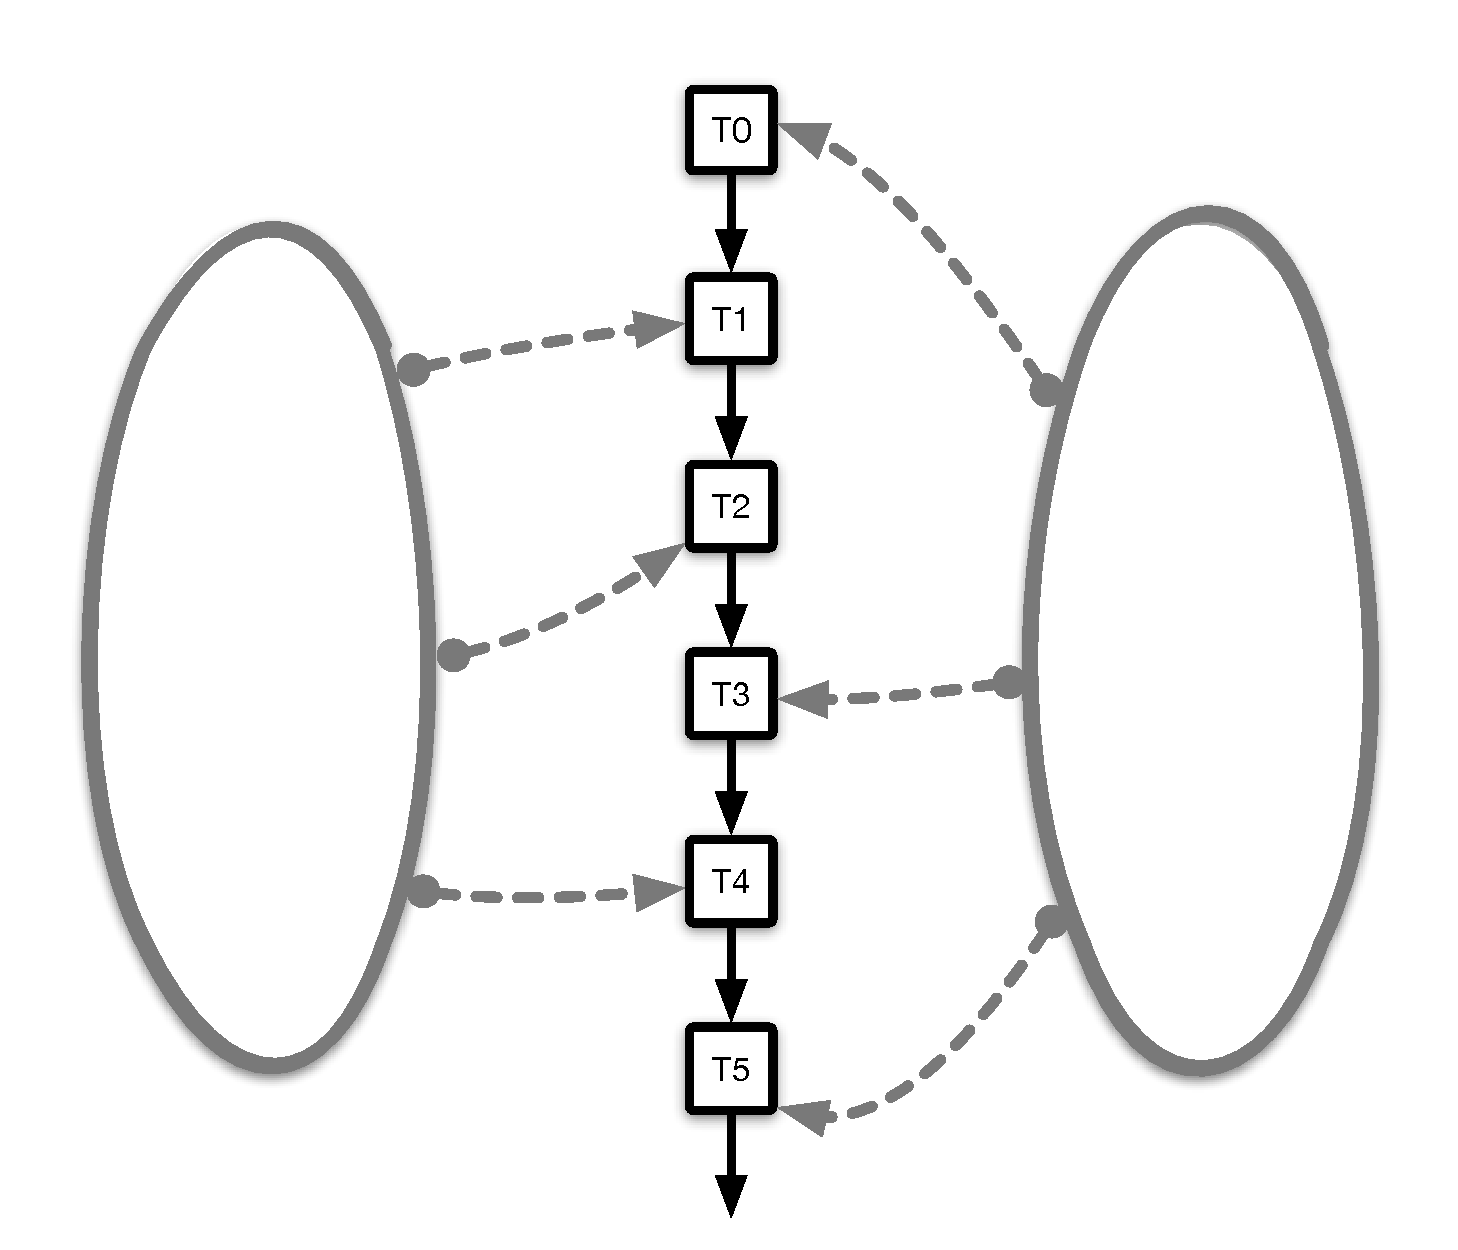
\includegraphics[height=4cm]{res/before-cloud.pdf}
\caption{\label{fig:relink:intro:before}}
\end{subfigure} \hfill
\begin{subfigure}[t]{0.48\textwidth}
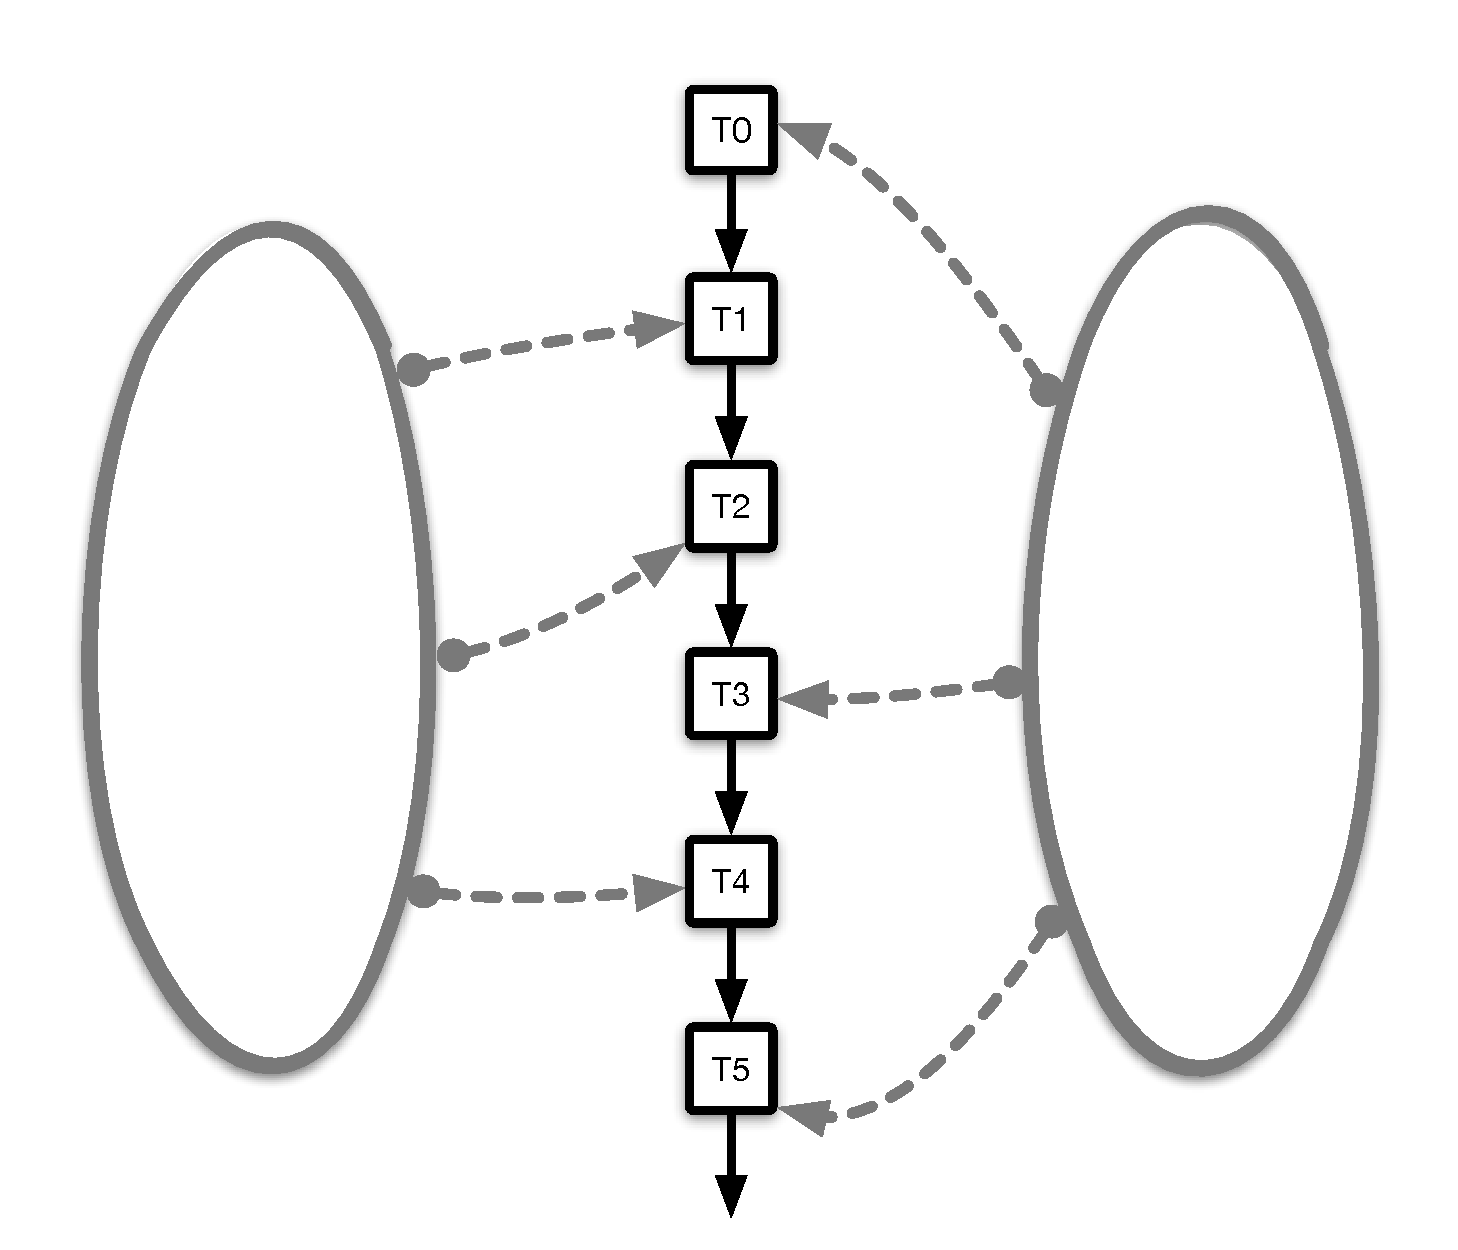
\includegraphics[height=4cm]{res/before-cloud.pdf}
\caption{\label{fig:relink:intro:after}} % Logical $\neq$ Real Time order, snapshot OK}
\end{subfigure}%
%
\caption{\label{fig:relink:intro} Placeholder for a general
  picture. The list ordering the events $T_0-T_5$ is permutted from
  (a) to (b), while preserving the event ownership: $T_1$, $T_2$ and
  $T_4$ have been executed---and are thus owned---by the specified
  thread (aka.~self), while $T_0$, $T_3$ and $T_5$ are executed by the
  interfering threads (aka.~other).}
\end{figure}


% Treating time as space 
Encoding temporal information by way of representing it as mutable
state allows us to use FCSL off-the-shelf to verify example
programs. In particular, FCSL has been implemented in the proof
assistant Coq, and we have fully mechanized the proof of Jayanti's
algorithm~\cite{CoqFiles}.

% \gad{I don't like the sound of some clients. But, I don't want to say
%   we have mechanized all the clients-- because the one using {\sf
%     hide} is not implemented.}

%
%We have previously applied FCSL to non-trivial concurrent data
%structures~\cite{SergeyNB+ESOP15}, including
%graphs~\cite{SergeyNB+PLDI15} and non-linearizable
%structures~\cite{SergeyNBD+OOPSLA16}. However, it was surprising to
%discover that the same logic can be applied to an algorithm such as
%Jayanti's, whose correctness argument requires dynamic reordering of
%terminated events.

\begin{comment}
While several recent Hoare logics have targeted concurrent programs
with non-thread-local and future-dependent linearization
points~\cite{LiangF+PLDI13,TuronDB+ICFP13}, they only allowed to
establish a procedure's LP position based on the observations made
\emph{during} the procedure's execution, \ie, scoped within
its \emph{region}.
%
However, a number of modern concurrent data structures exhibit
executions whose linearization order can only be established
\emph{after} the involved overlapping procedure calls have
terminated~\cite{HerlihyW+TOPLAS90, Jayanti+STOC05,
  DoddsHK+POPL15}. We call the linearization points of such executions
\emph{non-regional}, and our method is the first that provides a logic
for reasoning about non-regional linearization points.

\gad{The last statement might not be \it{entirely} true, Turon \etal
  do verify {\sf
    conditional-CAS}~\cite{HarrisFP+DISC02,FraserH+TOPLAS07} in
  CARESL's POPL'13 paper~\cite{TuronTABD+POPL13}, which is {\it
    supposed} to be non-regional as well. I've got to check the paper
  again to see how they do it.}
%
%% This was other of Ralf's remarks after the talk}}

\gad{More non-regional references we might want to mention, Elimination
  Queues. Gotta fetch a reference!}

The rest of the paper is organized as
follows. Section~\ref{sc:overview} describes Jayanti's algorithm, and
Sections~\ref{sc:formal} and~\ref{sc:implementation} show how the
auxiliary state and code can be designed to provide local
specs for it. Section~\ref{sc:proof} discusses the important
aspects of the correctness proof, and Section~\ref{sc:clients} shows
how to reason about clients. Section~\ref{sc:related} discusses the
related work.

\end{comment}


%We make an
%interesting parallel with linearizability, as this auxiliary state has
%to keep track of both beginning and ending times of an operation, for
%the purposes of the proof, although one of the endpoints can be
%omitted in the specs, which we present in the abstract form in Section
%4, along with the commentary of the formal proof. 
%
%This is the first proof of Jayanti's algorithm in a formal program
%logic. 
%
%Moreover, the proof is mechanized in in Coq.
%
%\an{Maybe not in Coq.}
%
%% In Section 4, we illustrate that the same specs can be ascribed to at
%% least one more snapshot implementation.
%
%
%before concluding (Section~6).
%
%Following the old adage that a method is a trick which worked at least
%twice, this lends credence to the claim that our snapshot API is
%canonical. We illustrate how the specs works in a several simple
%client program scenarios.
%
%\gad{WRT the Coq mechanization: Note that PODC's submission page
%  expects a .pdf file. Then if we provide code, it will have to be
%  available on-line. That could save us some time to try to push it
%  after the deadline but, it would be a risky enterprise. I'd rather
%  go safe and claim the mechanization is a work in progress. There is
%  no rebuttal period to argue back that we have finished it either.}

%\gad{ We should remember to point out the fact that unlike
%  linearizability proofs, we do not track the timestamp of all events,
%  but rather a few selected events. Moreover, our specs only need to
%  expose the timestamps of atomic write events in the histories, as
%  the only scanner timestamp that we are interested in, the
%  linearization point of the last scanner, is stored only in the
%  internal auxiliary state.  We need to spin this fact in our favor
%  here, and stress it later in Section~\ref{sc:formal} in further
%  detail.}


%% INTRO

\section{Introduction}
\label{sc:intro} 
   
Formal verification of concurrent objects commonly requires reasoning
about linearizability~\cite{HerlihyW+TOPLAS90}. This is a standard
correctness criterion whereby a concurrent execution of an object's
procedures is proved equivalent, via a simulation argument, to some
sequential execution. The clients of the object can be verified under
the sequentiality assumption, rather than by inlining the procedures
and considering their interleavings. Linearizability is often
established by describing the \emph{linearization points} (LP) of the
object, which are points in time where procedures take place,
\emph{logically}.  In other words, even if the procedure physically
executes across a time interval, exhibiting its linearization point
enables one to pretend, for reasoning purposes, that it occurred
instantaneously (\ie, atomically); hence, an interleaved execution of
a number of procedures can be reduced to a sequence of atomic events.

Reasoning about linearization points can be tricky. Many times, a
linearization point of a procedure is not \emph{local}, but may appear
in another procedure or thread. Equally bad, linearization points'
place in time may not be determined statically, but may vary based on
the past, and even future, \emph{run-time} information, thus
complicating the simulation arguments. A particularly troublesome case
is when run-time information influences the logical order of a
procedure that has already terminated.
%
This paper presents a novel approach to specification of concurrent
objects, in which the dynamic and non-local aspects inherent to
linearizability can be represented in a procedure-local and
thread-local manner. 

%\subparagraph{Reasoning about concurrent clients.}

The starting point of our idea is to realize what are the
shortcomings of linearizability as a canonical specification method
for concurrent objects.
%
Consider, for instance, the following two-threaded program manipulating
a correct implementation of stack by invoking its \texttt{push}
and \texttt{pop} methods, which are atomic, \ie, linearizable:
%
\begin{center}
\begin{tabular}{l || l}
\texttt{push(3);} & \texttt{push(4)}
\\
\texttt{t1 := pop(); } & \texttt{t2 := pop();}
\end{tabular} 
\end{center}
%
Assuming that the execution started in an empty stack, we would like
to derive that it returns an empty stack and \texttt{(t1, t2)} is
either \texttt{(3, 4)} or \texttt{(4, 3)}.
%
Linearizability of the stack guarantees that the overall trace of
\texttt{push}/\texttt{pop} calls is coherent with respect to a
sequential stack execution. However, it does not capture
\emph{client}-specific partial knowledge about the \emph{ordering} of
particular \texttt{push}/\texttt{pop} invocations in sub-threads,
which is what allows one to prove the desired result as a composition
of separately-derived partial specifications of the left and the right
thread.

This thread-local information, necessary for compositional reasoning
about clients, can be captured in a form of \emph{auxiliary
  state}~\cite{OwickiG+CACM76} (a generalization of \emph{history
  variables}~\cite{AbadiL+lics88}), widely used in Hoare-style
specifications of concurrent
objects~\cite{SergeyNB+ESOP15,LeyWildN+POPL13,JungSSSTBD+POPL15,JungKBD+ICFP16}. A
testament of expressivity of Hoare-style logics for concurrency with
rich auxiliary state are the recent results in verification of
fine-grained data structures with helping~\cite{SergeyNB+ESOP15},
concurrent graph manipulations~\cite{SergeyNB+PLDI15},
barriers~\cite{JungKBD+ICFP16,DoddsJPSB+TOPLAS16}, and even
\emph{non-linearizable} concurrent objects~\cite{SergeyNBD+OOPSLA16}.

Although designed to capture information about events that happened
concurrently \emph{in the past} (hence the original name \emph{history
  variables}), auxiliary state is known to be of little use for
reasoning about data structures with \emph{speculative} executions, in
which the ordering of past events may depend on other events happening
in the \emph{future}. Handling such data structures requires
specialized metatheory~\cite{LiangF+PLDI13} that does not provide
convenient abstractions such as auxiliary state for client-side
proofs. This is one reason why the most expressive client-oriented
concurrency logics to date avoid reasoning about speculative data
structures altogether~\cite{JungKBD+ICFP16}.

\subsubsection*{Our contributions}

The surprising result we present in this paper is that by allowing
certain \emph{internal} (\ie,~not observable by clients) manipulations
with the auxiliary state, we can use an existing program logic for
concurrency, like, \eg,
FCSL~\cite{NanevskiLSD+ESOP14,SergeyNB+PLDI15}, to specify and verify
algorithms whose linearizability argument requires speculations, \ie,
depends on the \emph{dynamic reordering} of events based on run-time
information from the future.
%
% and especially, reordering of terminated events.
%
To showcase this idea, we provide a new specification (spec) and the
first formal proof of a very sophisticated snapshot algorithm due to
Jayanti~\cite{Jayanti+STOC05}, whose linearizability proof exhibits
precisely such kind of dependence.

While we specify Jayanti's algorithm by means of a separation-style
logic, the spec nevertheless achieves the same general goals as
linearizability, combined with the benefits of compositional
Hoare-style reasoning.
%
In particular, our Hoare triple specs expose the logical atomicity of
Jayanti's methods (Section~\ref{sc:formal}), while hiding their true
fine-grained and physically non-atomic nature.  The approach also
enables that the separation logic reasoning is naturally applied to
clients (Section~\ref{sc:clients}).
%
Similarly to linearizability, our clients can reason out of
procedures' spec, not code. We can also ascribe the same spec to
different snapshot algorithms, without modifying client's code or
proof.

In more detail, our approach works as follows.
%
We use shared auxiliary state to record, as a list of timed events
(\eg, writes occurring at a given time), the logical order in which
the object's procedures are perceived to execute, each instantaneously
(Section~\ref{sc:auxiliaries}). Tracking this time-related information
through state enables us to specify its dynamic aspects. We can use
\emph{auxiliary code} to mutate the logical order \emph{in place},
thereby permuting the logical sequencing of the procedures, as may be
needed when some run-time event occurs
(Sections~\ref{sc:implementation} and~\ref{sc:proof}). This mutation
is similar to updating pointers to reorder a linked list, except that
it is executed over auxiliary state storing time-related data, rather
than over real state. This is why we refer to the idea as
\emph{linking-in-time}.

% Treating time as space 
Encoding temporal information by way of representing it as mutable
state allows us to use FCSL off-the-shelf to verify example
programs. In particular, FCSL has been implemented in the proof
assistant Coq, and we have fully mechanized the proof of Jayanti's
algorithm. The latter artifact, which is available for download from
the FCSL project website~\cite{FCSL:Project}, has been unanimously
accepted by ECOOP 2017's AEC.

% We have previously applied FCSL to non-trivial concurrent data
%structures~\cite{SergeyNB+ESOP15}, including
%graphs~\cite{SergeyNB+PLDI15} and non-linearizable
%structures~\cite{SergeyNBD+OOPSLA16}. However, it was surprising to
%discover that the same logic can be applied to an algorithm such as
%Jayanti's, whose correctness argument requires dynamic reordering of
%terminated events.

%
%% \gad Macros to refer to sbnapshot's pointers and line-numbers are
%% defined together with the Figure in

%\newcommand{\fx}{\text{fx}}
%\newcommand{\fy}{\text{fy}}
%\newcommand{\x}{\text{x}}
%\newcommand{\y}{\text{y}}
%\newcommand{\s}{\text{S}}

\newcommand{\fx}{\mathit{fx}}
\newcommand{\fy}{\mathit{fy}}
\newcommand{\x}{x}
\newcommand{\y}{y}
\newcommand{\s}{S}

%%\begin{wrapfigure}[9]{r}[0pt]{0.4\textwidth} 
%% \begin{figure}
%% %
%% \centering
%% \begin{tabular}{l l l}
%% %
%% %  
%% \begin{minipage}[l]{.30\textwidth}
%% \begin{alltt}
%% \num{1}  write (p, v): () \{
%% \num{2}    \act{write} (p, v);
%% \num{3}    b <- \act{read} (S);
%% \num{4}    \textbf{if} b 
%% \num{5}    \textbfthen \act{transfer} (p, v);
%% \num{6}    \textbf{else skip};\}
%% \end{alltt} 
%% \end{minipage}
%% %
%% & \hfill
%% %
%% \begin{minipage}[l]{.6\textwidth}
%% \begin{alltt}
%% \num{1}  scan (): \(A {\times} A\)  \{
%% \num{2}    \act{write} (S, true);
%% \num{3}    \act{write} (fx,\( \bot\));
%% \num{4}    \act{write} (fy,\( \bot\));
%% \num{5}    vx <- \act{read} (x);
%% \num{6}    vy <- \act{read} (y);
%% \num{7}    \act{write}(S, false);
%% \num{8}    ox <- \act{read} (fx);
%% \num{9}    oy <- \act{read} (fy);
%% \num{10}   \textbf{let} rx = \textbf{if} ox \(\neq \bot\) \textbfthen ox \textbf{else} vx;  
%% \num{11}   \textbf{let} ry = \textbf{if} oy \(\neq \bot\) \textbfthen oy \textbf{else} vy;  
%% \num{11}   \act{relink}(rx, ry);
%% \num{12}   \textbf{return} (rx, ry);
%% \end{alltt} 
%% \end{minipage}
%% %
%% \end{tabular}
%% %
%% \caption{Jayanti's single-scanner, single-writer snapshot algorithm}
%% \label{fig:jayanti}
%% \end{figure}
%\end{wrapfigure}

\newcommand{\actwrite}[2]{{#1}\,{:=}\,{#2}}

% The following version saves a little more space
\begin{figure}
%
\centering
\begin{tabular}{c@{\ \ \ \ \ }c}
%  
\begin{minipage}[t][3.7cm][t]{.5\textwidth}
\small
\begin{alltt}
\num{1} write (p : ptr, v : \(A\)) \{
\num{2}  \actwrite{p}{v};
\num{3}  b \tbnd \act{read}(S);
\num{4}  if b 
\num{5}  then \actwrite{(f_of p)}{v}
\num{6}  {else return} \}

  f_of (p : ptr) \{
   return p = x ? fx : fy \}
\end{alltt}
\end{minipage}
%
&
\begin{minipage}[t][3.7cm][t]{.5\textwidth}
\small
\begin{alltt}
\num{ 7} scan (): \(A {\times} A\)  \{
\num{ 8}  \actwrite{S}{true};
\num{ 9}  \actwrite{fx}{\(\bot\)}; \actwrite{fy}{\(\bot\)};
\num{10}  vx \tbnd \act{read}(x); vy \tbnd \act{read}(y);
\num{11}  \actwrite{S}{false};
\num{12}  ox \tbnd \act{read}(fx); oy \tbnd \act{read}(fy);
\num{13}  rx \tbnd if (ox \(\neq\bot\)) then ox {else} vx;  
\num{14}  ry \tbnd if (oy \(\neq\bot\)) then oy {else} vy;  
\num{15}  return (rx, ry) \}
\end{alltt} 
\end{minipage}
%
\end{tabular}
%
\caption{Jayanti's single-scanner/single-writer snapshot algorithm.}
\label{fig:jayanti-snapshot}
\end{figure}



\newcommand{\jywrite}{\texttt{write}\xspace}
\newcommand{\jyscan}{\texttt{scan}\xspace}

\section{Verification challenge and main ideas}
\label{sc:overview}


Jayanti's snapshot algorithm~\cite{Jayanti+STOC05} provides the
functionality of a shared array of size $m$, operated on by two
procedures: \jywrite, which stores a given value into an element, and
\jyscan, which returns the array's contents. We use the
\emph{single-writer}/\emph{single-scanner} version of the algorithm.
which assumes that at most one thread writes into an element, and at
most one thread invokes the scanner, at any given time. In other
words, there is a scanner lock and $m$ per-element locks. A thread
that wants to scan, has to acquire the scanner lock first, and a
thread that wants to write into element $i$ has to acquire the $i$-th
element lock. However, scanning and writing into different elements
can proceed concurrently.
% 
%where a thread acquires a writer lock for a particular element before
%writing into it, and a scanner before scanning. A scanner lock does
%not preclude writing, and a writer lock for an element does not
%preclude scanning, or writing into other elements. 
This is the simplest of Jayanti's algorithms, but it already exhibits
linearization points of dynamic nature. We also restrict the array
size to $m\,{=}\,2$ (\ie, we consider two pointers $\x$ and $\y$,
instead of an array). This removes some tedium from verification, but
exhibits the same conceptual challenges.
 
The difficulty in this snapshot algorithm is ensuring that the scanner
returns the most recent snapshot of the memory. A naive scanner, which
simply reads $\x$ and $\y$ in succession, is unsound. To see why,
consider the following scenario, starting with $\x=5$, $\y=0$. The
scanner reads $\x$, but before it reads $\y$, another thread preempts
it, and changes $\x$ to $2$ and, subsequently, $\y$ to $1$. The
scanner continues to read $\y$, and returns $\x=5, \y=1$, which was
never the contents of the memory. Moreover, $(\x, \y)$, changed from
$(5,0)$ to $(2, 0)$ to $(2, 1)$ as a result of distinct
non-overlapping writes; thus, it is impossible to find a linearization
point for the scan because linearizability only permits reordering of
non-overlapping operations.

%\ab{Remove rest?} by dynamically reordering non-overlapping
%operations, as permitted by linearizability (though we show further
%below a scenario when {\jyscan} is justified in returning a pair that
%was not the contents of the memory).

%\gad{Do we make the latter example a graph/ figure somehow? We have
%  done so for the slides}

To ensure a sound snapshot, Jayanti's algorithm internally keeps
additional \emph{forwarding pointers} $\fx$ and $\fy$, and a boolean
\emph{scanner bit} $\s$. The implementation is given in
Figure~\ref{fig:jayanti-snapshot}.\footnote{Following Jayanti, we
  simplify the presentation and omit the locking code that ensures the
  single-writer/single-scanner setup. Of course, in our Coq
  development~\cite{CoqFiles}, we make the locking explicit.}
%
The intuition is as follows. A writer storing $v$ into $p$
(line~\lineWrtWrt), will additionally store $v$ into the forwarding
pointer for $p$ (line~\lineWrtFwd), provided $S$ is set. If the
scanner missed the write and instead read the old value of $p$
(lines~\lineScanReadsX--\lineScanReadsY), it will have a chance to
catch $v$ via the forwarding pointer
(lines~\lineScanReadsFX--\lineScanReadsFY). The scanner bit $S$ is
used by writers (line~\lineWrtChk) to detect a scan in progress, and
forward $v$.

{
%\setlength{\belowcaptionskip}{-5pt} 
\begin{figure}[t]
%
\captionsetup[subfigure]{justification=centering}
\centering  
\begin{subfigure}[t]{1\textwidth}
\centering
\begin{tabular}{l || l || l}
  \texttt{l: }\texttt{write (x,2);}\quad &
   \multirow{2}{*}{\texttt{c: scan ()}}\quad & 
    \multirow{2}{*}{\texttt{r: write (x,3)}}  \\
  \phantom{\texttt{l: }}\texttt{write (y,1)} & &   
\end{tabular}
\caption{\label{fig:weird:code}Parallel composition of three threads \texttt{l, c, r}.}
\end{subfigure}\\

\begin{subfigure}[b]{1\textwidth}
\begin{tabular}{l@{\hfill} l@{\hfil}}
\begin{minipage}[t]{0.5\textwidth}
\begin{alltt}
 \num{1}  c: \actwrite{S}{true}
 \num{2}  c: \actwrite{fx}{\(\bot\)}
 \num{3}  c: \actwrite{fy}{\(\bot\)}
 \num{4}  c: \act{read}(x)  // vx <- 5
 \num{5}  c: \act{read}(y)  // vy <- 0
 \num{6}  l: \actwrite{x}{2}
 \num{7}  l: \act{read}(S)  // b <- true
 \num{8}  l: \actwrite{fx}{2} 
 \num{9}  l: return ()
\num{10}  r: \actwrite{x}{3}
\end{alltt}
\end{minipage}
&
\begin{minipage}[t]{0.33\textwidth}
\begin{alltt}
\num{11} l: \actwrite{y}{1}
\num{12} l: \act{read}(S)  // b <- true
\num{13} l: \actwrite{fy}{1}
\num{14} l: return ()
\num{15} c: \actwrite{S}{false}
\num{16} r: \act{read}(S)  // b <- false
\num{17} r: return ()
\num{18} c: \act{read}(fx) // ox <- 2
\num{19} c: \act{read}(fy) // oy <- 1
\num{20} c: return (2,1)
\end{alltt} 
\end{minipage}
%
\end{tabular}
\caption{\label{fig:weird:exec} A possible interleaving of the threads
  in~(\subref{fig:weird:code}).}
\end{subfigure}
\caption{\label{fig:weird} An example leading to a scanner miss.%
}
\end{figure}
}

 
As Jayanti proves, this implementation is linearizable. Informally,
every overlapping calls to \jywrite~and \jyscan~can be rearranged to
appear as if they occurred sequentially.  To illustrate, consider the
program in Figure~\ref{fig:weird:code}, and one possible interleaving
of its primitive memory operations in Figure~\ref{fig:weird:exec}. The
threads {\tt l}, {\tt c}, and {\tt r}, start with $\x = 5, \y = 0$.
%
The thread {\tt c} is scheduled first, and through lines~1--5 sets the
scanner bit, clears the forwarding pointers, and reads $\x = 5, \y =
0$. Then {\tt l} intervenes, and in lines~6--9, overwrites
$\x$ with $2$, and seeing $\s$ set, forwards $2$ to $\fx$. Next, {\tt
  r} and {\tt l} overlap, writing $3$ into $\x$ and $1$ into
$\y$. However, while $1$ gets forwarded to $\fy$ (line 13), $3$ is not
forwarded to $\fx$, because $\s$ was turned off in line 15 (\ie, the
scan is no longer in progress). Hence, when {\tt c} reads the
forwarded values (lines 18, 19), it returns $\x = 2, \y = 1$.

While $\x\,{=}\,2, \y\,{=}\,1$ was never the contents of the memory,
returning this snapshot is nevertheless justified because we can
\emph{pretend} that the scanner \emph{missed} {\tt r}'s write of
$3$. Specifically, the events in Figure~\ref{fig:weird:exec} can be
\emph{reordered} to represent the following sequential execution.
%
\begin{equation}
\mathtt{write\, (x, 2);\ write\, (y,1);\ scan\, ();\ write\, (x,
  3)} \label{eq:lin}
\end{equation}
The client programs cannot discover that a different scheduling
actually took place in real time, because they can access the internal
state of the algorithm only via interface methods, \jywrite~and \jyscan.

This kind of temporal reordering is the most characteristic aspect of
linearizability proofs, which typically describe the reordering by
listing the linearization points of each procedure. At a linearization
point, the procedure's operations can be spliced into the execution
history as an uninterrupted chunk. For example, in Jayanti's proof,
the linearization point of \jyscan~is at line~\lineScanUnsetsS\ in
Figure~\ref{fig:jayanti-snapshot}, where the scanner bit is unset. The
linearization point of \jywrite, however, may vary. If
\jywrite~starts before an overlapping \jyscan's line~\lineScanUnsetsS,
and moreover, the \jyscan~misses the \jywrite---note the dynamic and
future-dependent nature of this property---, then \jywrite~should
appear after {\tt scan}; that is, the \jywrite's linearization point
is right after \jyscan's linearization point at line~\lineScanUnsetsS.
%
Otherwise, \jywrite's linearization point is at line~\lineWrtWrt.
%
In the former case, \jywrite~exactly has a non-local and
future-dependent linearization point, because the decision on the
logical order of this \jywrite~depends on the execution of \jyscan~in
a different thread, and only \emph{after} the execution
of \jywrite~has terminated.
%
For instance, in Figure~\ref{fig:weird:exec} the execution
of \jywrite~in \texttt{r} terminates at step 17, yet, in Jayanti's
proof, the decision to linearize this \jywrite\ after the
overlapping \jyscan\ is taken at line~18, when the \jyscan\ reads the
value from the previous \jywrite.

%% \gad{Well, the non-regional argument is subtle and here is used with
%%   the wrong example: In this particular case, although the scanner bit
%%   is unset later at 15, the LP' of {\tt l} is fixed at line~11
%%   regardless of the future -- witnessed by the fact that it finishes
%%   green. The non-regionality argument has to be made about the
%%   position of the write to \x done by {\tt r}, which is the write that
%%   is relinked.}

%% \gad{When {\tt r} finishes in line~18, it's position in the final
%%   order is not settled as it depends on the scanners future: this
%%   write is missed by the scanner, and has to be relinked. This
%%   example, though showcases why relink is needed and how it works it
%%   does not showcase non-regionality: when 18 finishes, you have the
%%   information in lines 1-18 to determine that his position will be
%%   changed by scan before the end, so it can be linearized in line 18.}

\begin{figure}[t]
%\captionsetup[subfigure]{justification=centering}
\begin{subfigure}[t]{0.49\textwidth}
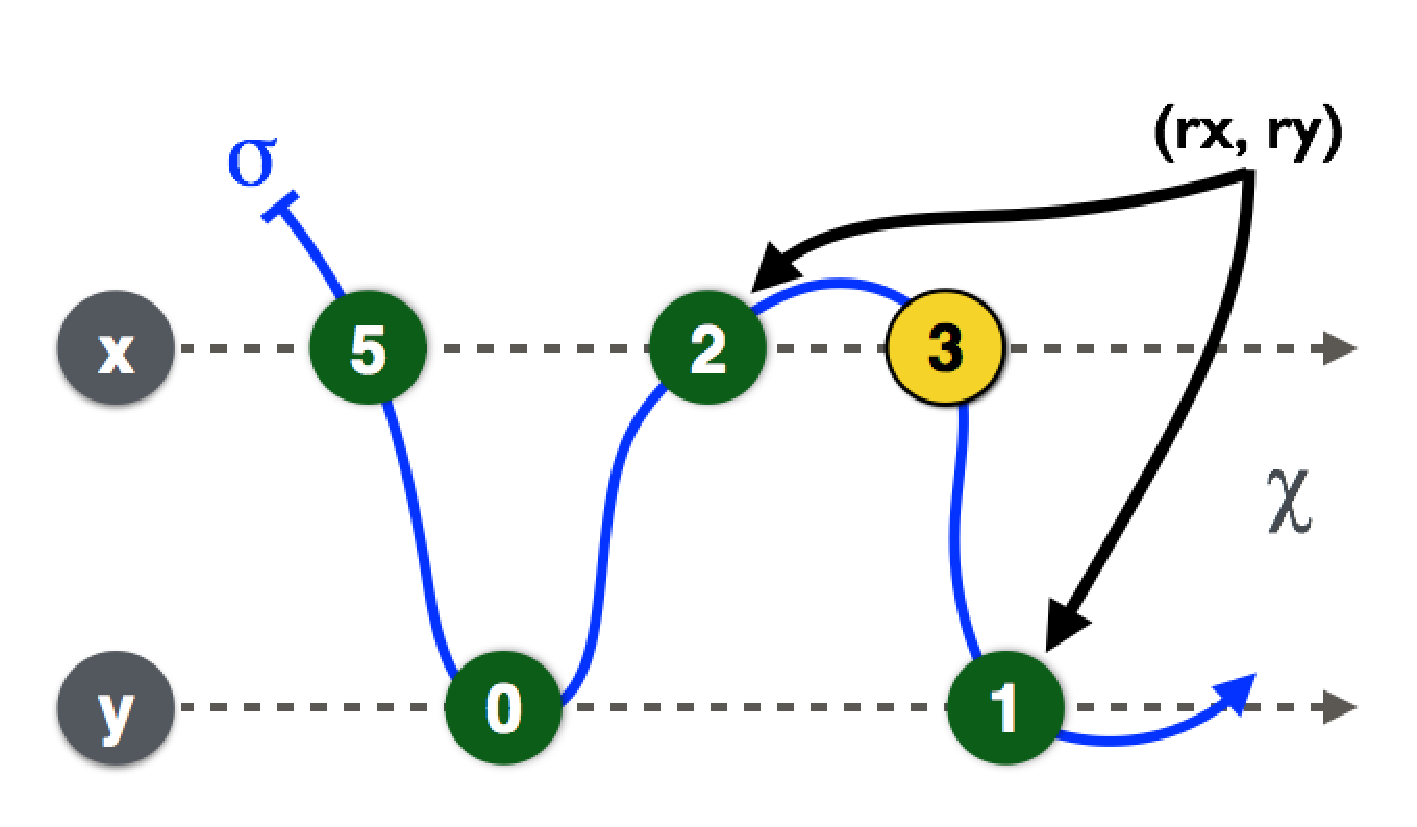
\includegraphics[width=6.1cm]{relink-before3.pdf}
\caption{\label{fig:reorder:before}} % Logical $=$ Real Time order, not a snapshot}
\end{subfigure} \hfill
\begin{subfigure}[t]{0.49\textwidth}
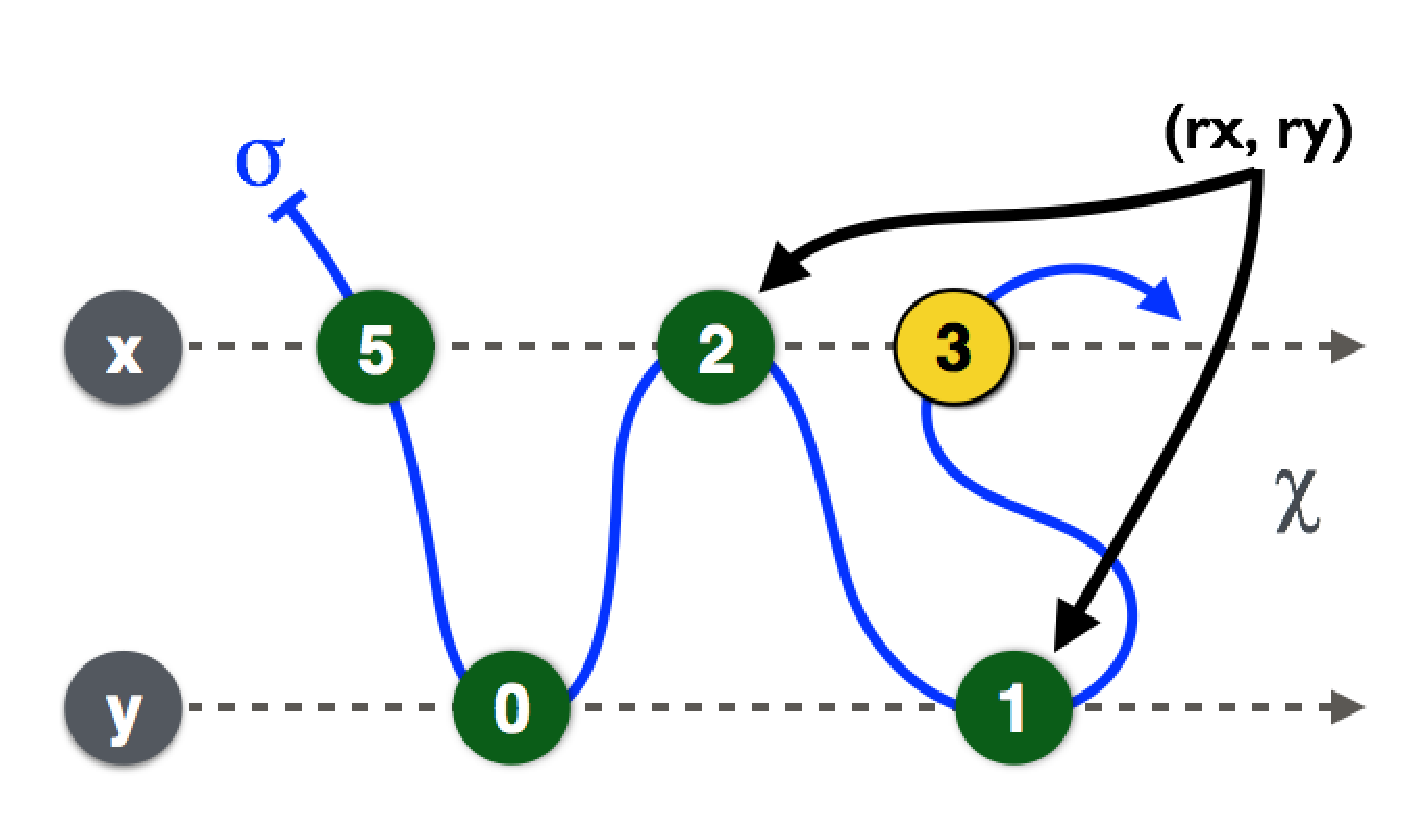
\includegraphics[width=6.1cm]{relink-after3.pdf}
\caption{\label{fig:reorder:after}} % Logical $\neq$ Real Time order, snapshot OK}
\end{subfigure}%
%
\caption{\label{fig:reorder} Changing the logical ordering (solid line
  $\ordlist$) of write events from (5, 0, 2, 3, 1) in
  (\subref{fig:reorder:before}) to (5, 0, 2, 1, 3) in
  (\subref{fig:reorder:after}), to reconcile with {\tt scan} returning
  the snapshot $\x=2, \y=1$, upon missing the write of $3$. Dashed
  lines $\hist$ represent real-time ordering.}
\end{figure}


Obviously, the high-level pattern of the proof requires tracking the
\emph{logical ordering} of the \jywrite\ and \jyscan\ events, which
differs from their \emph{real-time ordering}. As the logical ordering
is inherently dynamic, depending on properties such as
\jyscan\ missing a \jywrite, we formalize it in Hoare logic, by
keeping it as a list of events in auxiliary state that can be
dynamically reordered as needed. For example, Figure~\ref{fig:reorder}
shows the situation in the execution of \jyscan~that we reviewed
above. We start with the (initializing) writes of $5$ and $0$ already
executed, and our program performs the writes of $2$, $3$ and $1$ in
the real time order shown by the position of the events on the dashed
lines. In Figure~\ref{fig:reorder:before}, the logical order
$\ordlist$ coincides with real-time order, but is unsound for the
snapshot $\x=2, \y=1$ that \jyscan~wants to return. In that case, the
auxiliary code with which we annotate \jyscan, will change the
sequence $\ordlist$ in-place, as shown in
Figure~\ref{fig:reorder:after}.

Our specification and verification challenge then lies in reconciling
the following requirements. First, we have to posit specs that
say that \jywrite\ performs a write, and \jyscan\ performs a scan of
the memory, with the operations executing in a single logical
moment. Second, we need to implement the event reordering discipline
so that a method call only reorders events that overlap with it; the
logical order of the past events should be preserved. This will be
accomplished by introducing yet further structures into the auxiliary
state and code. Finally, the specs must hide the specifics of
the reordering discipline, which should be internal to the snapshot
object. Different snapshot implementations should be free to implement
different reorderings, without changing the method specs.


%Our challenge then lies in reconciling the following two conflicting
%requirements. First, we need to implement the reordering discipline so
%that the subsequent calls to \jywrite~and \jyscan~preserve the
%established logical order of the past events. This will be
%accomplished by introducing yet further structures into the auxiliary
%state and code. Second, we have to engineer Hoare triples for
%\jywrite~and \jyscan~to be \emph{intuitive} and \emph{helpful} to
%clients, but also to \emph{not expose} the specifics of the reordering
%discipline, which is internal to the snapshot object\footnotemark.
%%We discuss these issues next.
%\footnotetext{\ie we want to give the methods {\it principal} specifications}




%% OVERVIEW

%% Macros to refer to snapshot's pointers and line-numbers are
%% defined together with the Figure in

\newcommand{\fx}{\mathit{fx}}
\newcommand{\fy}{\mathit{fy}}
\newcommand{\x}{x}
\newcommand{\y}{y}
\newcommand{\s}{S}

%%% Macros for Snapshot pointers

%% Jayanti's Snapshot Algorithm
\newcommand{\fwdp}[1]{(\esc{fwd}~#1)}
\newcommand{\aleksfwdp}[1]{\esc{fwd}~#1}

\begin{figure}[t]
%
\centering
\begin{tabular}[t]{l@{\ \ \ }l}
%  
\begin{minipage}[t]{.4\textwidth}
\[
\begin{array}{rl}
\num{1}~ & \esc{write}\ (p,\, v)\ \{ \\ 
\num{2}~ & ~~~ \actwrite{p}{v}; \\
\num{3}~ & ~~~ b \tbnd \act{read}(\s);\\
\num{4}~ & ~~~ \kw{if}\ b\\
\num{5}~ & ~~~ \kw{then}\ \actwrite{\fwdp{p}}{v}\}\\
& \\
& \\
& \esc{fwd}\ (p : \esc{ptr})\ \{ \\
& ~~~ \kw{return}\ (p = x)\ \esc{?}\ \fx \esc{:}\ \fy\ \}
\end{array}
\]
\end{minipage}
%
&
\begin{minipage}[t]{.6\textwidth}
\[
\begin{array}{rl}
\num{6}~  & \esc{scan}\ :\ (A \times A)\ \{\\ 
\num{7}~  & ~~~~ \actwrite{\s}{\esc{true}};\\
\num{8}~  & ~~~~ \actwrite{\fx}{\bot};\\
\num{9}~  & ~~~~ \actwrite{\fy}{\bot}; \\
\num{10}~ & ~~~~ \var{vx} \tbnd \act{read}(\x);\\
\num{11}~ & ~~~~ \var{vy} \tbnd \act{read}(\y);\\
\num{12}~ & ~~~~ \actwrite{\s}{\esc{false}};\\
\num{13}~ & ~~~~ \var{ox} \tbnd \act{read}(\fx);\\
\num{14}~ & ~~~~ \var{oy} \tbnd \act{read}(\fy);\\
\num{15}~ & ~~~~ \var{rx} \tbnd \kw{if}\ (\var{ox} \neq\bot)\ \kw{then}\ \var{ox}\
                          \kw{else}\ \var{vx};\\  
\num{16}~ & ~~~~ \var{ry} \tbnd \kw{if}\ (\var{oy} \neq\bot)\ \kw{then}\ \var{oy}\
                          \kw{else}\ \var{vy};\\  
\num{17}~ & ~~~~ \kw{return}~(\var{rx},\var{ry})\}\\
\end{array}
\]
\end{minipage}
%
\end{tabular}
%
\caption{Jayanti's single-scanner/single-writer snapshot algorithm.}
\label{fig:jayanti-snapshot}
\end{figure}

% Macros for Line Numbers

\def\lineWrtStarts{1}
\def\lineWrtWrt{2}
\def\lineWrtChk{3}
\def\lineWrtIf{4}
\def\lineWrtFwd{5}
\def\lineWrtFnz{5'}

\def\lineScanStarts{6}
\def\lineScanSetsS{7}
\def\lineScanClearsX{8}
\def\lineScanClearsY{9}
\def\lineScanReadsX{10}
\def\lineScanReadsY{11}
\def\lineScanUnsetsS{12}
\def\lineScanReadsFX{13}
\def\lineScanReadsFY{14}
\def\lineScanChoosesRX{15}
\def\lineScanChoosesRY{16}
\def\lineScanRelinks{17}

\newcommand{\jywrite}{\texttt{write}\xspace}
\newcommand{\jyscan}{\texttt{scan}\xspace}

%%% OVERVIEW

\section{Verification challenge and main ideas}
\label{sc:overview}

Jayanti's snapshot algorithm~\cite{Jayanti+STOC05} provides the
functionality of a shared array of size $m$, operated on by two
procedures: \jywrite, which stores a given value into an element, and
\jyscan, which returns the array's contents. We use the
\emph{single-writer}/\emph{single-scanner} version of the algorithm.
which assumes that at most one thread writes into an element, and at
most one thread invokes the scanner, at any given time. In other
words, there is a scanner lock and $m$ per-element locks. A thread
that wants to scan, has to acquire the scanner lock first, and a
thread that wants to write into element $i$ has to acquire the $i$-th
element lock. However, scanning and writing into different elements
can proceed concurrently.
% 
%where a thread acquires a writer lock for a particular element before
%writing into it, and a scanner before scanning. A scanner lock does
%not preclude writing, and a writer lock for an element does not
%preclude scanning, or writing into other elements. 
This is the simplest of Jayanti's algorithms, but it already exhibits
linearization points of dynamic nature. We also restrict the array
size to $m\,{=}\,2$ (\ie, we consider two pointers $\x$ and $\y$,
instead of an array). This removes some tedium from verification, but
exhibits the same conceptual challenges.
 
The difficulty in this snapshot algorithm is ensuring that the scanner
returns the most recent snapshot of the memory. A na\"{i}ve scanner, which
simply reads $\x$ and $\y$ in succession, is unsound. To see why,
consider the following scenario, starting with $\x=5$, $\y=0$. The
scanner reads $\x$, but before it reads $\y$, another thread preempts
it, and changes $\x$ to $2$ and, subsequently, $\y$ to $1$. The
scanner continues to read $\y$, and returns $\x=5, \y=1$, which was
never the contents of the memory. Moreover, $(\x, \y)$, changed from
$(5,0)$ to $(2, 0)$ to $(2, 1)$ as a result of distinct
non-overlapping writes; thus, it is impossible to find a linearization
point for the scan because linearizability only permits reordering of
overlapping operations.

To ensure a sound snapshot, Jayanti's algorithm internally keeps
additional \emph{forwarding pointers} $\fx$ and $\fy$, and a Boolean
\emph{scanner bit} $\s$. The implementation is given in
Figure~\ref{fig:jayanti-snapshot}.\footnote{Following Jayanti, we
  simplify the presentation and omit the locking code that ensures the
  single-writer/single-scanner setup. Of course, in our Coq
  development~\cite{FCSL:Project}, we make the locking explicit.}
%
The intuition is as follows. A writer storing $v$ into $p$
(line~\lineWrtWrt), will additionally store $v$ into the forwarding
pointer for $p$ (line~\lineWrtFwd), provided $S$ is set. If the
scanner missed the write and instead read the old value of $p$
(lines~\lineScanReadsX--\lineScanReadsY), it will have a chance to
catch $v$ via the forwarding pointer
(lines~\lineScanReadsFX--\lineScanReadsFY). The scanner bit $S$ is
used by writers (line~\lineWrtChk) to detect a scan in progress, and
forward $v$.

%{
%\setlength{\belowcaptionskip}{-5pt} 
\begin{figure}[t]
%
\captionsetup[subfigure]{justification=centering}
\centering  
\begin{subfigure}[t]{1\textwidth}
\centering
\begin{tabular}{l || l || l}
  \texttt{l: }\texttt{write (x,2);}\quad &
   \multirow{2}{*}{\texttt{c: scan ()}}\quad & 
    \multirow{2}{*}{\texttt{r: write (x,3)}}  \\
  \phantom{\texttt{l: }}\texttt{write (y,1)} & &   
\end{tabular}
\caption{\label{fig:weird:code}Parallel composition of three threads \texttt{l, c, r}.}
\end{subfigure}\\

\begin{subfigure}[b]{1\textwidth}
\begin{tabular}{l@{\hfill} l@{\hfil}}
\begin{minipage}[t]{0.5\textwidth}
\begin{alltt}
 \num{1}  c: \actwrite{S}{true}
 \num{2}  c: \actwrite{fx}{\(\bot\)}
 \num{3}  c: \actwrite{fy}{\(\bot\)}
 \num{4}  c: \act{read}(x)  // vx <- 5
 \num{5}  c: \act{read}(y)  // vy <- 0
 \num{6}  l: \actwrite{x}{2}
 \num{7}  l: \act{read}(S)  // b <- true
 \num{8}  l: \actwrite{fx}{2} 
 \num{9}  l: return ()
\num{10}  r: \actwrite{x}{3}
\end{alltt}
\end{minipage}
&
\begin{minipage}[t]{0.33\textwidth}
\begin{alltt}
\num{11} l: \actwrite{y}{1}
\num{12} l: \act{read}(S)  // b <- true
\num{13} l: \actwrite{fy}{1}
\num{14} l: return ()
\num{15} c: \actwrite{S}{false}
\num{16} r: \act{read}(S)  // b <- false
\num{17} r: return ()
\num{18} c: \act{read}(fx) // ox <- 2
\num{19} c: \act{read}(fy) // oy <- 1
\num{20} c: return (2,1)
\end{alltt} 
\end{minipage}
%
\end{tabular}
\caption{\label{fig:weird:exec} A possible interleaving of the threads
  in~(\subref{fig:weird:code}).}
\end{subfigure}
\caption{\label{fig:weird} An example leading to a scanner miss.%
}
\end{figure}
}

%%% TRACES FIG.

\begin{figure}[t]
%
\captionsetup[subfigure]{justification=centering}
\centering  
\begin{subfigure}[t]{1\textwidth}
\centering
\begin{tabular}{l || l || l}
  \texttt{l: }\texttt{write (x,2);}\quad &
   \multirow{2}{*}{\texttt{c: scan ()}}\quad & 
    \multirow{2}{*}{\texttt{r: write (x,3)}}  \\
  \phantom{\texttt{l: }}\texttt{write (y,1)} & &   
\end{tabular}
\caption{\label{fig:weird:code}Parallel composition of three threads
  \texttt{l, c, r}.}
\end{subfigure}\\

\begin{subfigure}[b]{1\textwidth}
\begin{tabular}{l@{\hfill} l@{\hfil}}
\begin{minipage}[t]{0.5\textwidth}
\begin{alltt}
 \num{1}  c: \actwrite{S}{true}
 \num{2}  c: \actwrite{fx}{\(\bot\)}
 \num{3}  c: \actwrite{fy}{\(\bot\)}
 \num{4}  c: \act{read}(x)  // vx <- 5
 \num{5}  c: \act{read}(y)  // vy <- 0
 \num{6}  l: \actwrite{x}{2}
 \num{7}  l: \act{read}(S)  // b <- true
 \num{8}  l: \actwrite{fx}{2} 
 \num{9}  l: return ()
\num{10}  r: \actwrite{x}{3}
\end{alltt}
\end{minipage}
&
\begin{minipage}[t]{0.33\textwidth}
\begin{alltt}
\num{11} l: \actwrite{y}{1}
\num{12} l: \act{read}(S)  // b <- true
\num{13} l: \actwrite{fy}{1}
\num{14} l: return ()
\num{15} c: \actwrite{S}{false}
\num{16} r: \act{read}(S)  // b <- false
\num{17} r: return ()
\num{18} c: \act{read}(fx) // ox <- 2
\num{19} c: \act{read}(fy) // oy <- 1
\num{20} c: return (2,1)
\end{alltt} 
\end{minipage}
%
\end{tabular}
\caption{\label{fig:weird:exec} A possible interleaving of the threads
  in~(\subref{fig:weird:code}).}
\end{subfigure}
\caption{\label{fig:weird} An example leading to a scanner miss.%
}
\end{figure}
%%%

As Jayanti proves, this implementation \emph{is} linearizable. Informally,
every overlapping calls to \jywrite~and \jyscan~can be rearranged to
appear as if they occurred sequentially.  To illustrate, consider the
program in Figure~\ref{fig:weird:code}, and one possible interleaving
of its primitive memory operations in Figure~\ref{fig:weird:exec}. The
threads {\tt l}, {\tt c}, and {\tt r}, start with $\x = 5, \y = 0$.
%
The thread {\tt c} is scheduled first, and through lines~1--5 sets the
scanner bit, clears the forwarding pointers, and reads $\x = 5, \y =
0$. Then {\tt l} intervenes, and in lines~6--9, overwrites
$\x$ with $2$, and seeing $\s$ set, forwards $2$ to $\fx$. Next, {\tt
  r} and {\tt l} overlap, writing $3$ into $\x$ and $1$ into
$\y$. However, while $1$ gets forwarded to $\fy$ (line 13), $3$ is not
forwarded to $\fx$, because $\s$ was turned off in line 15 (\ie, the
scan is no longer in progress). Hence, when {\tt c} reads the
forwarded values (lines 18, 19), it returns $\x = 2, \y = 1$.

While $\x\,{=}\,2, \y\,{=}\,1$ was never the contents of the memory,
returning this snapshot is nevertheless justified because we can
\emph{pretend} that the scanner \emph{missed} {\tt r}'s write of
$3$. Specifically, the events in Figure~\ref{fig:weird:exec} can be
\emph{reordered} to represent the following sequential execution:
%
\begin{equation}
\hfill \mathtt{write\, (x, 2);\ write\, (y,1);\ scan\, ();\ write\, (x,
  3)}\hfill \label{eq:lin}
\end{equation}
%
Importantly, the client programs have no means to discover that a
different scheduling actually took place in real time, because they
can access the internal state of the algorithm only via interface
methods, \jywrite~and \jyscan.

This kind of temporal reordering is the most characteristic aspect of
linearizability proofs, which typically describe the reordering by
listing the linearization points of each procedure. At a linearization
point, the procedure's operations can be spliced into the execution
history as an uninterrupted chunk. For example, in Jayanti's proof,
the linearization point of \jyscan~is at line~\lineScanUnsetsS\ in
Figure~\ref{fig:jayanti-snapshot}, where the scanner bit is unset. The
linearization point of \jywrite, however, may vary. If
\jywrite~starts before an overlapping \jyscan's line~\lineScanUnsetsS,
and moreover, the \jyscan~misses the \jywrite---note the dynamic and
future-dependent nature of this property---, then \jywrite~should
appear after {\tt scan}; that is, the \jywrite's linearization point
is right after \jyscan's linearization point at line~\lineScanUnsetsS.
%
Otherwise, \jywrite's linearization point is at line~\lineWrtWrt.
%
In the former case, \jywrite~exactly has a non-local and
future-dependent linearization point, because the decision on the
logical order of this \jywrite~depends on the execution of \jyscan~in
a different thread. This decision takes effect on
lines~\lineScanReadsFX--\lineScanReadsFY, which can take place
\emph{after} the execution of \jywrite~has terminated.
%
For instance, in Figure~\ref{fig:weird:exec} the execution
of \jywrite~in \texttt{r} terminates at step 17, yet, in Jayanti's
proof, the decision to linearize this \jywrite\ after the
overlapping \jyscan\ is taken at line~18, when the \jyscan\ reads the
value from the previous \jywrite.

%\begin{figure}[t]
%\captionsetup[subfigure]{justification=centering}
\begin{subfigure}[t]{0.49\textwidth}
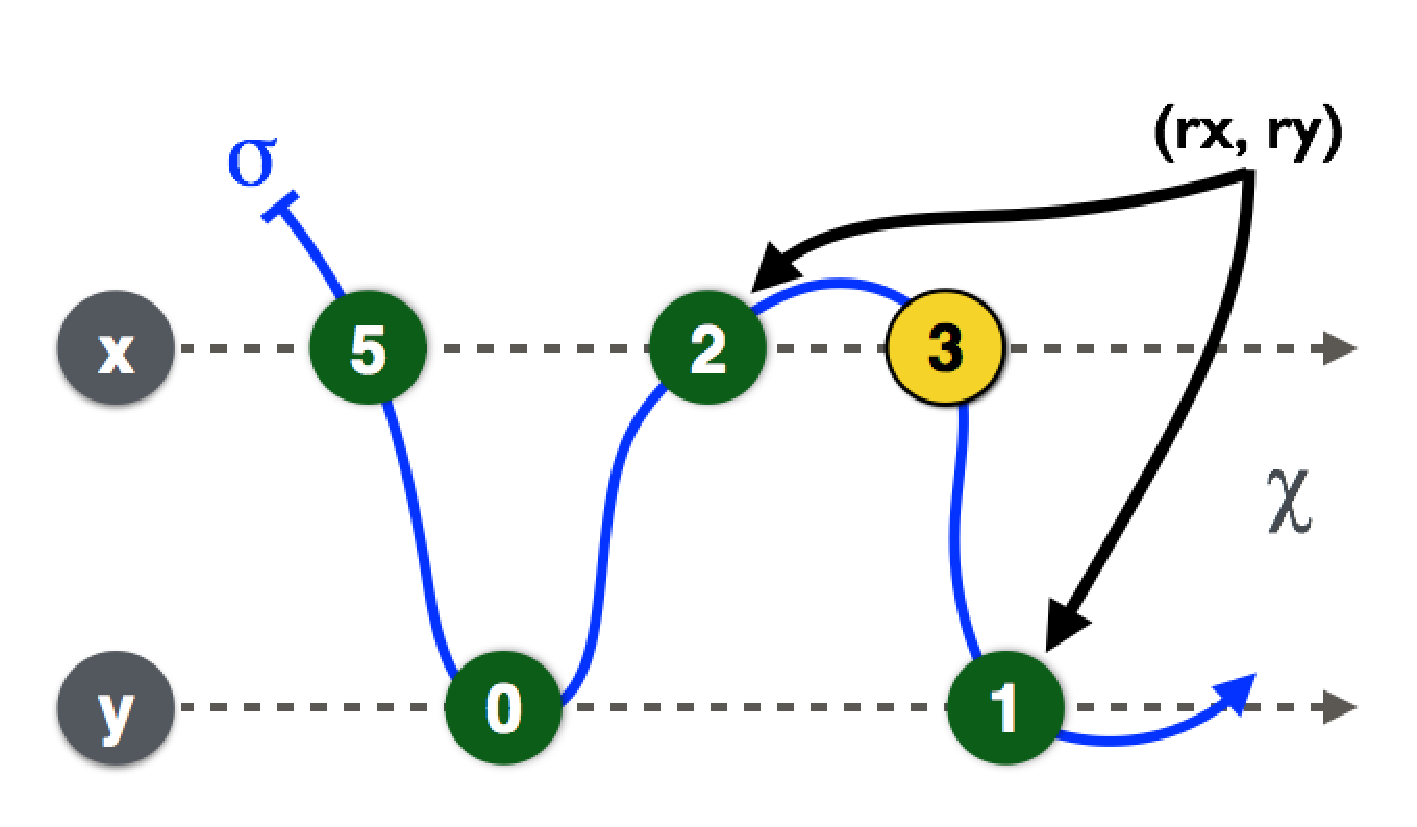
\includegraphics[width=6.1cm]{relink-before3.pdf}
\caption{\label{fig:reorder:before}} % Logical $=$ Real Time order, not a snapshot}
\end{subfigure} \hfill
\begin{subfigure}[t]{0.49\textwidth}
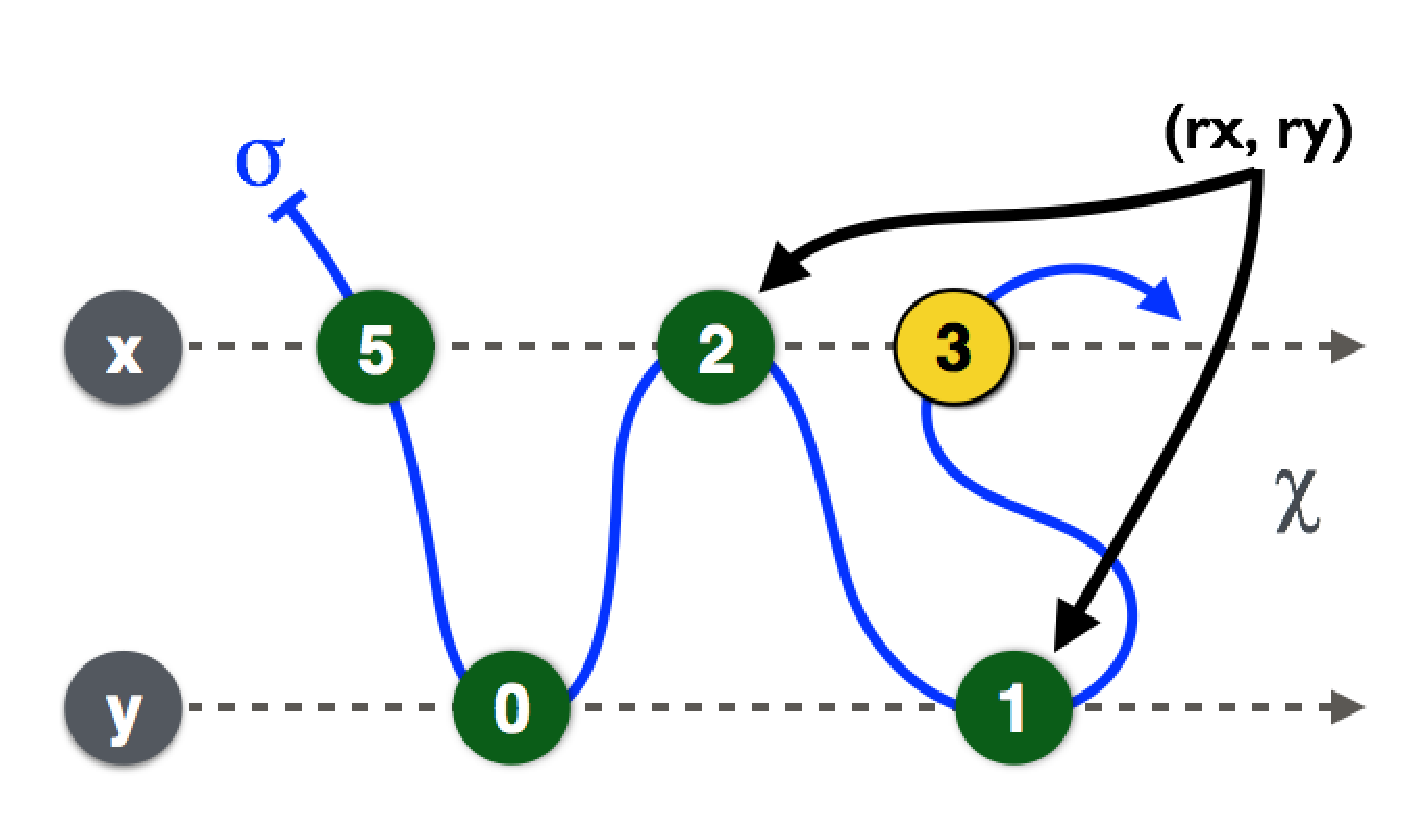
\includegraphics[width=6.1cm]{relink-after3.pdf}
\caption{\label{fig:reorder:after}} % Logical $\neq$ Real Time order, snapshot OK}
\end{subfigure}%
%
\caption{\label{fig:reorder} Changing the logical ordering (solid line
  $\ordlist$) of write events from (5, 0, 2, 3, 1) in
  (\subref{fig:reorder:before}) to (5, 0, 2, 1, 3) in
  (\subref{fig:reorder:after}), to reconcile with {\tt scan} returning
  the snapshot $\x=2, \y=1$, upon missing the write of $3$. Dashed
  lines $\hist$ represent real-time ordering.}
\end{figure}

%% RELINK FIG.

\begin{figure}[t]
\begin{subfigure}[t]{0.49\textwidth}
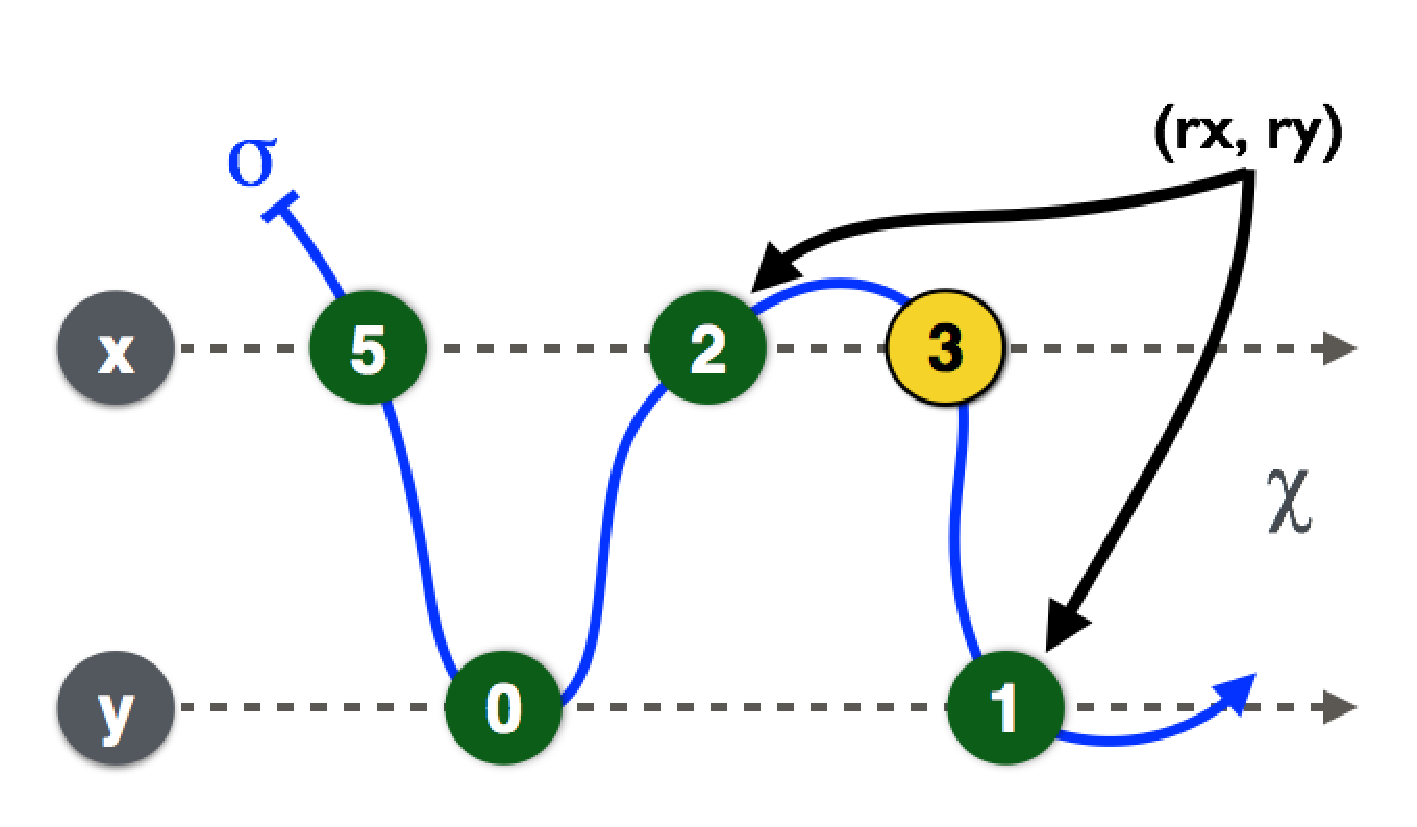
\includegraphics[width=6.1cm]{relink-before3.pdf}
\caption{\label{fig:reorder:before}} % Logical $=$ Real Time order, not a snapshot}
\end{subfigure} \hfill
\begin{subfigure}[t]{0.49\textwidth}
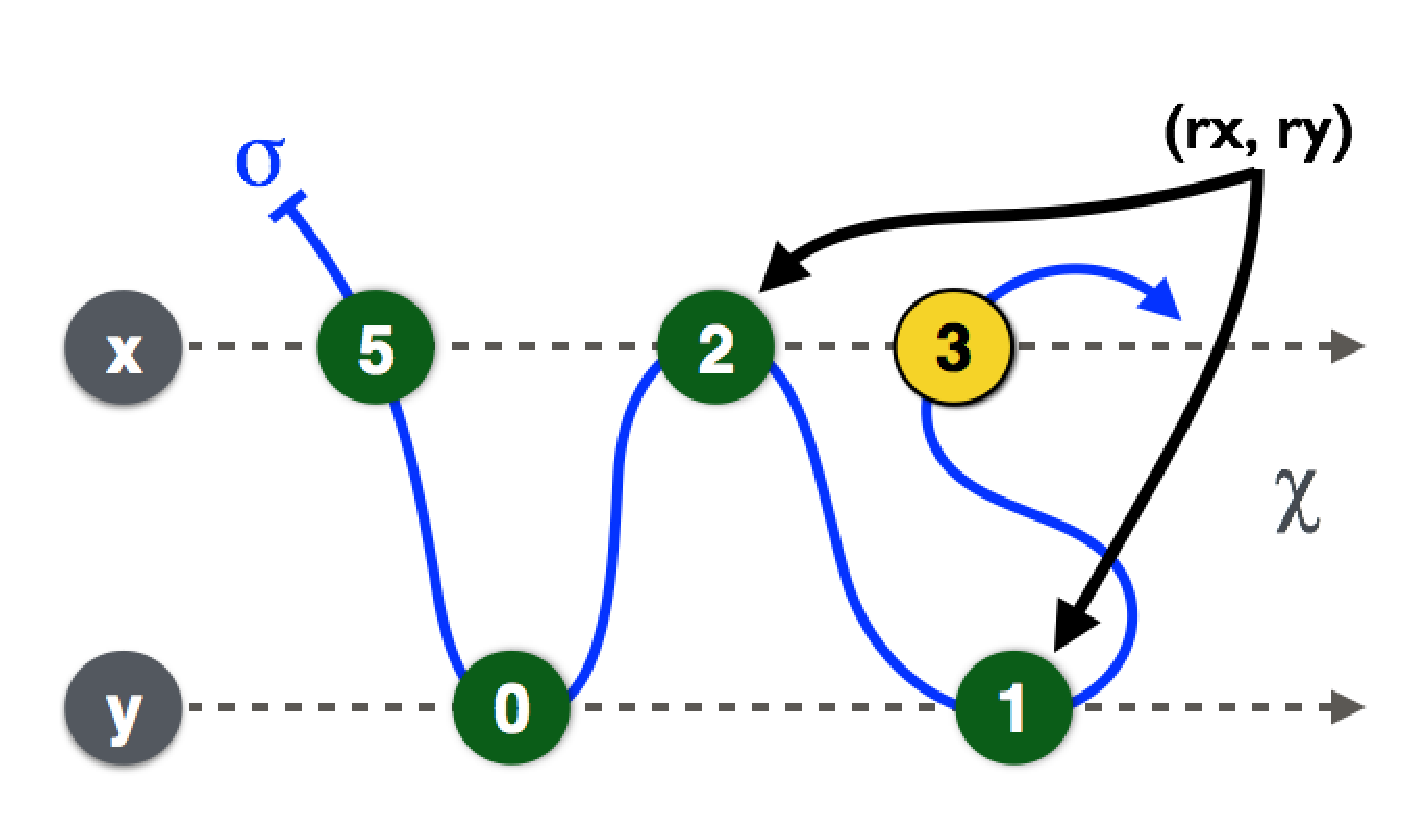
\includegraphics[width=6.1cm]{relink-after3.pdf}
\caption{\label{fig:reorder:after}} % Logical $\neq$ Real Time order, snapshot OK}
\end{subfigure}%
%
\caption{\label{fig:reorder} Changing the logical ordering (solid line
  $\ordlist$) of write events from (5, 0, 2, 3, 1) in
  (\subref{fig:reorder:before}) to (5, 0, 2, 1, 3) in
  (\subref{fig:reorder:after}), to reconcile with {\tt scan} returning
  the snapshot $\x=2, \y=1$, upon missing the write of $3$. Dashed
  lines $\hist$ represent real-time ordering.}
\end{figure}


Obviously, the high-level pattern of the proof requires tracking the
\emph{logical ordering} of the \jywrite\ and \jyscan\ events, which
differs from their \emph{real-time ordering}. As the logical ordering
is inherently dynamic, depending on properties such as
\jyscan\ missing a \jywrite, we formalize it in Hoare logic, by
keeping it as a list of events in auxiliary state that can be
dynamically reordered as needed. For example, Figure~\ref{fig:reorder}
shows the situation in the execution of \jyscan~that we reviewed
above. We start with the (initializing) writes of $5$ and $0$ already
executed, and our program performs the writes of $2$, $3$ and $1$ in
the real time order shown by the position of the events on the dashed
lines. In Figure~\ref{fig:reorder:before}, the logical order
$\ordlist$ coincides with real-time order, but is unsound for the
snapshot $\x=2, \y=1$ that \jyscan~wants to return. In that case, the
auxiliary code with which we annotate \jyscan, will change the
sequence $\ordlist$ in-place, as shown in
Figure~\ref{fig:reorder:after}.

Our specification and verification challenge then lies in reconciling
the following requirements. First, we have to posit specs that
say that \jywrite\ performs a write, and \jyscan\ performs a scan of
the memory, with the operations executing in a single logical
moment. Second, we need to implement the event reordering discipline
so that a method call only reorders events that overlap with it; the
logical order of the past events should be preserved. This will be
accomplished by introducing yet further structures into the auxiliary
state and code. Finally, the specs must hide the specifics of
the reordering discipline, which should be internal to the snapshot
object. Different snapshot implementations should be free to implement
different re-orderings, without changing the method specs.

%Our challenge then lies in reconciling the following two conflicting
%requirements. First, we need to implement the reordering discipline
%so that the subsequent calls to \jywrite~and \jyscan~preserve the
%established logical order of the past events. This will be
%accomplished by introducing yet further structures into the auxiliary
%state and code. Second, we have to engineer Hoare triples for
%\jywrite~and \jyscan~to be \emph{intuitive} and \emph{helpful} to
%clients, but also to \emph{not expose} the specifics of the
%reordering discipline, which is internal to the snapshot
%object\footnotemark.
%%We discuss these issues next.
%\footnotetext{\ie we want to give the methods {\it principal}
%specifications}

%\section{Specification}
\label{sc:formal}

%% Auxiliary state defs

\def\histx{\hist_\x}
\def\histy{\hist_\y}
\def\histp{\hist_p}

\newcommand{\sx}{S_\x}
\newcommand{\sy}{S_\y}
\newcommand{\spp}{S_p}
\newcommand{\sss}{S_s}
\newcommand{\wx}{W_\x}
\newcommand{\wy}{W_\y}
\newcommand{\wpp}{W_p}

%\newcommand{\admissible}{\mathsf{fine}}

% Names for writer/scanner-states
\def\toff{t_{\mathsf{off}}}

%% \newcommand{\wInit}{\mathsf{W_{Off}}}
%% \newcommand{\wWrite}{\mathsf{W_{New}}}
%% \newcommand{\wDirty}{\mathsf{W_{Fwd}}}
%% \newcommand{\wClean}{\mathsf{W_{Done}}}

%% \newcommand{\sOn}{\mathsf{S_{On}}}
%% \newcommand{\sOff}{\mathsf{S_{Off}}}


\paragraph*{General considerations.}
%
For the purposes of specification and proof, we record a history of
the snapshot object as a set of entries of the form $t \mapsto (p,
v)$. The entry says that at time $t$ (a natural number), the value $v$
was written into the pointer $p$. We thus identify a write event with
a \emph{single} moment in time $t$, enabling the specs of
\jywrite\ and \jyscan\ to present the view that write events are
logically atomic.
%
Moreover, in the case of snapshots, we can ignore the scan events in
the histories. The latter do not modify the state in a way observable
by clients who can access the shared pointers only via interface
methods \jywrite\ and\ \jyscan.

We keep three auxiliary history variables. The history variables
$\histS$ and $\histO$ are local to the specified thread, and record
the \emph{terminated} write events carried out by the specified
thread, and that thread's interfering environment, respectively. We
refer to $\histS$ as the \emph{self}-history, and to $\histO$ as the
\emph{other}-history~\cite{LeyWildN+POPL13,NanevskiLSD+ESOP14,OPLSS:Notes,SergeyNB+ESOP15}. The role of 
$\histO$ is to enable the spec of \jywrite\ to situate the performed
write event within the larger context of past and ongoing writes, and
the spec of \jyscan\ to describe how it logically reordered the writes
that overlapped with it.
%

The third history variable $\histJ$ records the set of write events
that are in progress. These are events that have been initiated,
timestamped, and have executed their physical write to memory, but
have not terminated yet. It is an important component of our auxiliary
state design that when a write event terminates, it is moved from
$\histJ$ to the invoking thread's $\histS$, to indicate the
\emph{ownership} of the write by the invoking thread.
%
We name by $\hist$ the union $\histS \hunion \histO \hunion \histJ$,
which is the global history of the data structure. As common in
separation logic, the union is \emph{disjoint}, \ie, it is undefined
if the components contain duplicate timestamps. By the semantics of
our specs, $\hist$ is always defined, thus $\histS$, $\histO$ and
$\histJ$ never duplicate timestamps.

The real-time ordering of the timestamped events is the natural
numbers ordering on the timestamps. To track the \emph{logical}
ordering, we need further auxiliary notions.
%
The first is the auxiliary variable $\ordlist$, whose type is a
mathematical sequence. The sequence $\ordlist$ is a permutation of
timestamps from $\hist$ showing the logical ordering of the events in
$\hist$. We write $t_1 \tleq t_2$, and say that $t_1$ is logically
ordered before $t_2$, if $t_1$ appears before $t_2$ in $\ordlist$. The
sequence $\ordlist$ resides in joint state, and can be dynamically
modified by any thread. For example, the execution of the scanner may
reorder $\ordlist$, as shown in
Figure~\ref{fig:reorder:after}. Because $\ordlist$ is a sequence, the
order $\tleq$ is linear.

%
%In this sense, $\ordlist$ is the linkage in time for the snapshot
%algorithm, and it will be dynamically modified. 
%

Because sequence $\ordlist$ changes dynamically under interference, it
is not appropriate for specifications. Thus, our second auxiliary
notion is the \emph{partial} order $\stableorder$, a suborder of
$\tleq$ that is \emph{stable} in the following sense. It relates the
timestamps of events whose logical order has been determined,
\emph{and will not change in the future}. Thus $\stableorder$ can grow
over time, to add new relations between previously unrelated
timestamps, but cannot change the old relations.

%we require further a subset of ${\tleq}$, that is \emph{stable} in the
%following sense. This order relates the timestamps of events whose
%logical order has already been fixed, and will not change in the
%future. One can say that such events have been ``linearized''.  Being
%stable, $\stableorder$ can only grow over time to add new relations
%between previously unrelated timestamps, but cannot change the old
%relations.
%

To illustrate the distinction between the two orders, we refer to
Figure~\ref{fig:reorder:before}. There, $\ordlist$ represents the
linear order $5{-}0{-}2{-}3{-}1$, which changes in
Figure~\ref{fig:reorder:after} to $5{-}0{-}2{-}1{-}3$.
%
Since $1$ and $3$ exchange places, the stable order $\stableorder$
cannot initially relate the two. Thus, in
Figure~\ref{fig:reorder:before}, $\stableorder$ is represented by
the Hasse diagram as
$5{-}0{-}2{<}\!\begin{array}[c]{c}1\\ 3\end{array}$. In
Figure~\ref{fig:reorder:after}, the relation $1{-}3$ is added to this
partial order, making it the linear order $5{-}0{-}2{-}1{-}3$. Note
how the previous relations remain unchanged.

\newcommand{\scanned}[1]{\mathsf{scanned}\,#1}

The third auxiliary notion is the set $\scanned\stableorder$ of
timestamps. A write's timestamp is placed in $\scanned\stableorder$,
if that write has been observed by some scanner; that is, the written
value is returned in some snapshot, or has been rewritten by another
value that is returned in some snapshot. To illustrate, in the above
example, $\{5, 0, 2\} \subseteq \scanned\stableorder$.  Intuitively,
we want to model that after a write has been observed, the ordering of
the events logically preceding the write must be stabilized, and
moreover, must be a sequence. Thus,
%If $t \in \scanned\stableorder$, then all the events logically
%preceding $t$ should also satisfy the above property, thus
$\scanned\stableorder$ is a \emph{linearly ordered subset} of
$\stableorder$.\footnote{In terminology of linearizability, one may
  say that $\scanned\stableorder$ is the set of ``linearized''
  writes.}  The set $\scanned\stableorder$ can also be seen as
\emph{representing all the scans that have already been
  executed}. Such representation of scans allows us to avoid tracking
scan events directly in the history.

In the sequel, we concretize $\stableorder$ and
$\scanned\stableorder$ in terms of $\ordlist$ and other auxiliary
state. However, we keep the notions abstract in the method specs and
in client reasoning. This enables the use of different snapshot
algorithms, with the same specs, without invalidating the client
proofs. We also mention that $\ordlist$, $\stableorder$ and
$\scanned\stableorder$ can be encoded as user-level concepts in FCSL,
and require no new logic to be developed.

%%
%% \begin{equation}
%% \begin{array}{l}
%% \mathtt{write}\ (p : \mathtt{ptr}, n : \mathtt{int}) : 
%% \!\!\!\begin{array}[t]{l}
%% \{\hists = \hempty \wedge h \subseteq \histO
%%            \wedge \omega \subseteq {\stableorder}\}\\[3pt]
%% \{\exists t\ldot\, \hists = t \mapsto (p, n) \wedge h \subseteq \histO \wedge
%%   \omega \subseteq {\stableorder}\,{\wedge}\, h \subseteq H^{\hbox{}\sqsubsetneq_\ordlist t}\}
%% \end{array}\\
%% %
%% \mathtt{scan} : 
%% \!\!\!\begin{array}[t]{l}
%% \{\hists = \hempty \wedge\, h \subseteq \histO \wedge\,
%%           \omega \subseteq {\stableorder}\}\\[3pt]
%% \{\hists = \hempty \wedge\, h \subseteq \histO \wedge\, \omega \subseteq {\stableorder} \wedge\, \exists\, t\ldot\, %
%%            h \subseteq H^{\hbox{}\sqsubseteq_\ordlist t} \wedge\,
%%            \mathsf{chain}\ H^{\hbox{}\sqsubseteq_\ordlist t} \wedge\,
%%            r = \mathsf{eval}\ {H^{\hbox{}\sqsubseteq_\ordlist t}}\}
%% \end{array}
%% \end{array}
%% \label{eq:specs}
%% \end{equation}
%

\paragraph*{Snapshot specification.}
% The following version saves a little more space
\begin{figure}
%
\centering
\[
\begin{array}{l}
\mathtt{write}\ (p : \mathtt{ptr}, n : \mathtt{int}) : 
\!\!\!\begin{array}[t]{l}
\{\hists = \hempty \wedge h \subseteq \histO
           \wedge \omega \subseteq {\jleq}\}\\[3pt]
\{\exists t\ldot\, \hists = t \mapsto (p, n) \wedge h \subseteq \histO \wedge
  \omega \subseteq {\jleq}\,{\wedge}\, h \subseteq H^{\hbox{}\sqsubsetneq_\ordlist t}\}
\end{array}\\
%
\mathtt{scan} : 
\!\!\!\begin{array}[t]{l}
\{\hists = \hempty \wedge\, h \subseteq \histO \wedge\,
          \omega \subseteq {\jleq}\}\\[3pt]
          \{\hists = \hempty \wedge\, h \subseteq \histO \wedge\,
            \omega \subseteq {\jleq} \wedge\, \exists\, t\ldot\, %
             h \subseteq H^{\hbox{}\sqsubseteq_\ordlist t} \wedge\,
             \mathsf{chain}\ H^{\hbox{}\sqsubseteq_\ordlist t} \wedge\,
             r = \mathsf{eval}\ {H^{\hbox{}\sqsubseteq_\ordlist t}}\}
       \end{array}
\end{array}
\]
\caption{\label{fig:specs} Specification of {\tt write} and {\tt scan}
  methods.}
\end{figure}
 
%
Figure~\ref{fig:specs} presents our specs for \jyscan~and
\jywrite. These are partial correctness specs that describe how
the methods change the state from the precondition (first braces) to
the postcondition (second braces), possibly influencing the value $r$
that the procedure returns. We use VDM-style notation with unprimed
variables for the state before, and primed variables for the state
after the method executes. We use Greek letters for state-dependent
values that can be mutated by the method, and Latin letters for
immutable variables.
%
The component $C$ is a state transition system (STS) that describes the
state space of the algorithm, i.e, the invariants on the auxiliary and
real state, and the transitions, i.e., the allowed atomic mutations of
the state. For now, we keep $C$ abstract, but will define it in
Sections~\ref{sc:auxiliaries} and~\ref{sc:implementation}.
%
We denote by $\ideal{\stableorder}{t}$ the downward-closed set of
timestamps
$\ideal{\stableorder}{t} = \{ s \mid s\ {\stableorder}\ t \}$. Let
$\sideal{\stableorder}{t} = (\ideal{\stableorder}{t})\setminus\{t\}$.

%downward-closed wrt.~$\stableorder$:
%\begin{align*}
%%\label{eq:ideal-order} 
%\alekideal{\stableorder}{t} \eqdef \{ s \mid s\ {\stableorder}\ t \}\qquad\mbox{and}\qquad
%%\label{eq:sideal-order} 
%\aleksideal{\stableorder}{t} \eqdef
%  \{ s \mid s\ {\stableorder}\ t \wedge s \neq te\}
%\end{align*}

The spec for \jywrite\ says the following. The precondition starts
with the empty self history $\histS$, indicating that the procedure
has not made any writes. In the postcondition, a new write event $t
\mapsto (p, v)$ has been placed into $\histS'$. Thus, a call to
\jywrite\ wrote $v$ into pointer $p$. The timestamp $t$
is fresh, because $\histP$ does not contain duplicate timestamps.
%
%\histS$ and $\hist$ \ab{?} are always disjoint (by the
%semantics of FCSL triples). 
%
Moreover, the write appears as if it occurred atomically at time
$t$, thus capturing the logical atomicity of \jywrite.

The next conjunct, $\dom{\histO} \cup \scanned\stableorder \subseteq
\sideal{\stableorderP}{t}$, positions the write $t$ into the context
of other events. In particular, if $s \in \dom{\histO}$, \ie, if $s$
finished prior to invoking \jywrite, then $s$ is logically ordered
strictly before $t$. In other words, \jywrite\ cannot reorder prior
events that did not overlap with it. The definition of linearizability
contains a similar prohibition on reordering non-overlapping events,
but here, we capture it using a Hoare-style spec. For similar reasons,
we require that $\scanned\stableorder \subseteq
\sideal{\stableorderP}{t}$. As mentioned before,
$\scanned\stableorder$ represents all the scans that finished prior to
the call to \jywrite. Consequently, they do not overlap with
\jywrite\ in real time, and have to be logically ordered before $t$.

Notice what the spec of \jywrite\ \emph{does not prevent}. It is
possible that some event, say with a timestamp $s$, finishes in real
time before the call of \jywrite~at time $t$. Events $s$ and $t$ do
not overlap, and hence cannot be reordered; thus
$s\ {\stableorder}\ t$ always. However, the relationship of $s$ with
other events that ran concurrently with $s$, may be fixed only later,
thus supporting implementation of ``future-dependent'' nature, such as
Jayanti's.

%For example, in Figure~\ref{fig:reorder:before}, the event $3$ is
%ordered after $5$, $0$, and $2$, but its order wrt.~$1$ is determined
%only later.

%For example, if $s$ overlapped with some other event $s'$, it is
%possible for $s$ and $s'$ to not be immediately related in
%$\stableorder$. The relative ordering of $s$ and $s'$ may be
%determined after either of the events has terminated.  \ab{Can we give
%  an example here?}

In the case of \jyscan, we start and terminate with an empty $\histS$,
because \jyscan\ does not create any write events, and we do not track
scan events. However, when \jyscan\ returns the pair $r = (r_\x,
r_\y)$, we know that there exists a timestamp $t$ that describes when
the scan took place. This $t$ is the timestamp of the last write
preceding the call to \jyscan.

The postcondition says that $t$ is the moment in which the snapshot
was logically taken, by the conjunct $r =
\eval\ t\ \stableorderP\ \histP$.  Here, $\eval$ is a pure,
specification-level function that works as follows. First, it reorders
the entire real-time post-history $\histP$ according to logical
post-ordering $\stableorderP$. Then, it computes and returns the
values of $x$ and $y$ that would result from executing the write
events of such reordered history up to the timestamp $t$. For example,
if $t$ is the timestamp of event $1$ in
Figure~\ref{fig:reorder:after}, then $\eval\ t\ \stableorderP\ \histP$
would return $(2, 1)$. Hence, the conjunct says that
\jyscan\ performed a scan of $x$ and $y$, consistent with the ordering
$\stableorderP$, and returned the read values into $r$. The scan
appears as if it occurred atomically, immediately after time $t$, thus
capturing the atomicity of \jyscan.

%\ab{Can we connect with Figure 3b here?}

The next conjunct, $\dom{\hist} \subseteq \ideal{\stableorderP}{t}$,
says that the scanner returned a snapshot that is current, rather than
corresponding to an outdated scan. For example, referring to
Figure~\ref{fig:reorder}, if \jyscan\ is invoked after the events $2$
and $1$ have already executed, then \jyscan\ should not return the
pair $(5, 0)$ and have $t$ be the timestamp of the event $0$, because
that snapshot is outdated. Specifically, the conjunct says that the
write events from $\hist$ are ordered no later than $t$, similar to
the postcondition of \jywrite. However, while in \jywrite\ we
constrained the events from $\dom{\histO} \cup \scanned\stableorder$,
here we constrain the full global history $\hist = \histO \hunion
\histJ$. The addition of $\histJ$ shows that the scanner will observe
and order all of the write events that have been timestamped and
recorded in $\histJ$ (and thus, that have written their value to
memory), prior to the invocation of \jyscan.

Lastly, the conjunct $t \in \scanned\stableorderP$ explicitly says
that $t$ has been observed by the just finished call to scan.

Again, it is important what the spec does not prevent. It is possible
that the timestamp $t$ identified as the moment of the scan,
corresponds to a write that has been initiated, but has not yet terminated.
Despite being ongoing, $t$ is placed into $\scanned\stableorderP$
(\ie, $t$ is ``linearized''). Also, notice that the postcondition of
\jyscan\ actually specifies the ``linearization'' order of events that
are initiated by another method, namely \jywrite, thus supporting
implementations of ``non-local'' nature, such as Jayanti's.

We close the section with a brief discussion of how the specs are
used. Because $C$, $\stableorder$ and $\scanned$ are abstracted from
the clients, we need to provide an interface to work with them. The
interface consists of a number of properties showing how various
assertions interact, summarized in the statements below.

The first statement presents the invariants on the transitions of STS
$C$, often referred to as 2-state invariants.
%
Another way of working with such invariants is to include them in the
postcondition of every method.\footnote{In fact, this is what we
  currently do in our Coq files.} For simplicity, here we agglomerate
the properties, and use them implicitly in proofs as needed.
%
\begin{invariant}[Transition invariants]\label{inv:monotonicity}
In any program respecting the transitions of $C$: 
\begin{enumerate}
\item\label{inv:mono:hist} $\hist \subseteq \histP$, $\histS \subseteq
  \histSP$ and $\histO \subseteq \histOP$, and also $\stableorder
  \subseteq \stableorderP$.
\item\label{inv:mono:ideal} For every $s \in \scanned{\stableorder}$,
  $\ideal{\stableorder}{s} = \ideal{\stableorderP}{s}$.
\end{enumerate}
\end{invariant}

Invariant~\ref{inv:monotonicity}.\ref{inv:mono:hist} says that
histories and $\stableorder$ only grow, but does not insist that
$\histJ \subseteq \histJP$, as timestamps can be removed from $\histJ$
and transferred to $\histS$.
%
Invariant~\ref{inv:monotonicity}.\ref{inv:mono:ideal} says that if a
new event is added to increase $\stableorder$ to $\stableorderP$, that
event appears logically later than any $s \in
\scanned{\stableorder}$. In other words, once events are observed by a
scanner, and placed into $\scanned{\stableorder}$ in a certain order,
we cannot insert new events among them to modify the past observation.

The second statement exposes the properties of $\stableorder$ and
$\scanned$ that are used for client reasoning.
%
\begin{invariant}[Relating $\stableorder$ and $\scanned$]\label{lem:scanned}%
%The set $\scanned\, \stableorder$ satisfies the following properties:
%
\begin{enumerate}
 \item\label{lem:scan:total} if $ t_1 \in
   \scanned{\stableorder}$ and $t_2 \in \scanned{\stableorder}$, then
   $ t_1 \mathrel{\stableorder} t_2 \vee t_2 \mathrel{\stableorder}
   t_1 $ (linearity).
   
 \item \label{lem:scan:wkn} if $ t_2 \in
   \scanned{\stableorder}$ and $ t_1 \mathrel{\stableorder} t_2$, then
   $t_1 \in \scanned{\stableorder}$ (downward closure).

%\item[\textit{(principality???)}] \label{lem:scan:subset} if $ t \in
%  \scanned{\stableorder}$ then $\ideal{\stableorder}{t} \subseteq
%  \scanned{\stableorder}$.

\item \label{lem:scan:prefix} if $t \in
  \scanned{\stableorder}$ and $ \ideal{\stableorder}{t} =
  \ideal{\stableorderP}{t}$, then $t \in \scanned{\stableorderP}$ (principality).
  
\item \label{lem:scan:eval} if $t \in
  \scanned{\stableorder}$, $\ \hist \subseteq \histP$ and $
  \ideal{\stableorder}{t} = \ideal{\stableorderP}{t}$ then $ \eval\,
  t\, \stableorder\, \hist = \eval\, t\, \stableorderP\, \histP$. % (eval preservation).
\end{enumerate}
\end{invariant}




%% SPECS SECTION

\section{Specification}
\label{sc:formal}

%% Auxiliary state defs

\def\histx{\hist_\x}
\def\histy{\hist_\y}
\def\histp{\hist_p}

\newcommand{\sx}{S_\x}
\newcommand{\sy}{S_\y}
\newcommand{\spp}{S_p}
\newcommand{\sss}{S_s}
\newcommand{\wx}{W_\x}
\newcommand{\wy}{W_\y}
\newcommand{\wpp}{W_p}

%\newcommand{\admissible}{\mathsf{fine}}

% Names for writer/scanner-states
\def\toff{t_{\mathsf{off}}}

%% \newcommand{\wInit}{\mathsf{W_{Off}}}
%% \newcommand{\wWrite}{\mathsf{W_{New}}}
%% \newcommand{\wDirty}{\mathsf{W_{Fwd}}}
%% \newcommand{\wClean}{\mathsf{W_{Done}}}

%% \newcommand{\sOn}{\mathsf{S_{On}}}
%% \newcommand{\sOff}{\mathsf{S_{Off}}}


\subparagraph*{General considerations.}
%
For the purposes of specification and proof, we record a history of
the snapshot object as a set of entries of the form $t \mapsto (p,
v)$. The entry says that at time $t$ (a natural number), the value $v$
was written into the pointer $p$. We thus identify a write event with
a \emph{single} moment in time $t$, enabling the specs of
\jywrite\ and \jyscan\ to present the view that write events are
logically atomic.
%
Moreover, in the case of snapshots, we can ignore the scan events in
the histories. The latter do not modify the state in a way observable
by clients who can access the shared pointers only via interface
methods \jywrite\ and\ \jyscan.

We keep three auxiliary history variables. The history variables
$\histS$ and $\histO$ are local to the specified thread, and record
the \emph{terminated} write events carried out by the specified
thread, and that thread's interfering environment, respectively. We
refer to $\histS$ as the \emph{self}-history, and to $\histO$ as the
\emph{other}-history~\cite{LeyWildN+POPL13,NanevskiLSD+ESOP14,Nanevski+OPLSS16,SergeyNB+ESOP15}. The
role of $\histO$ is to enable the spec of \jywrite\ to situate the
performed write event within the larger context of past and ongoing
writes, and the spec of \jyscan\ to describe how it logically
reordered the writes that overlapped with it.
%
The third history variable $\histJ$ records the set of write events
that are in progress. These are events that have been initiated,
timestamped, and have executed their physical write to memory, but
have not terminated yet. It is an important component of our auxiliary
state design that when a write event terminates, it is moved from
$\histJ$ to the invoking thread's $\histS$, to indicate the
\emph{ownership} of the write by the invoking thread.
%
We name by $\hist$ the union $\histS \hunion \histO \hunion \histJ$,
which is the global history of the data structure. As common in
separation logic, the union is \emph{disjoint}, \ie, it is undefined
if the components contain duplicate timestamps. By the semantics of
our specs, $\hist$ is always defined, thus $\histS$, $\histO$ and
$\histJ$ never duplicate timestamps.

The real-time ordering of the timestamped events is the natural
numbers ordering on the timestamps. To track the \emph{logical}
ordering, we need further auxiliary notions.
%
The first is the auxiliary variable $\ordlist$, whose type is a
mathematical sequence. The sequence $\ordlist$ is a permutation of
timestamps from $\hist$ showing the logical ordering of the events in
$\hist$. We write $t_1 \tleq t_2$, and say that $t_1$ is logically
ordered before $t_2$, if $t_1$ appears before $t_2$ in $\ordlist$. The
sequence $\ordlist$ resides in joint state, and can be dynamically
modified by any thread. For example, the execution of the scanner may
reorder $\ordlist$, as shown in
Figure~\ref{fig:reorder:after}. Because $\ordlist$ is a sequence, the
order $\tleq$ is linear.

%
%In this sense, $\ordlist$ is the linkage in time for the snapshot
%algorithm, and it will be dynamically modified. 
%

Because sequence $\ordlist$ changes dynamically under interference, it
is not appropriate for specifications. Thus, our second auxiliary
notion is the \emph{partial} order $\stableorder$, a suborder of
$\tleq$ that is \emph{stable} in the following sense. It relates the
timestamps of events whose logical order has been determined,
\emph{and will not change in the future}. Thus $\stableorder$ can grow
over time, to add new relations between previously unrelated
timestamps, but cannot change the old relations.

%we require further a subset of ${\tleq}$, that is \emph{stable} in the
%following sense. This order relates the timestamps of events whose
%logical order has already been fixed, and will not change in the
%future. One can say that such events have been ``linearized''.  Being
%stable, $\stableorder$ can only grow over time to add new relations
%between previously unrelated timestamps, but cannot change the old
%relations.
%

To illustrate the distinction between the two orders, we refer to
Figure~\ref{fig:reorder:before}. There, $\ordlist$ represents the
linear order $5{-}0{-}2{-}3{-}1$, which changes in
Figure~\ref{fig:reorder:after} to $5{-}0{-}2{-}1{-}3$.
%
Since $1$ and $3$ exchange places, the stable order $\stableorder$
cannot initially relate the two. Thus, in
Figure~\ref{fig:reorder:before}, $\stableorder$ is represented by the
Hasse diagram $5{-}0{-}2{<}\!\begin{array}[c]{c}1\\ 3\end{array}$. In
Figure~\ref{fig:reorder:after}, the relation $1{-}3$ is added to this
partial order, making it the linear order $5{-}0{-}2{-}1{-}3$. Note
how the previous relations remain unchanged.

\newcommand{\scanned}[1]{\mathsf{scanned}\,#1}

The third auxiliary notion is the set $\scanned\stableorder$ of
timestamps. A write's timestamp is placed in $\scanned\stableorder$,
if that write has been observed by some scanner; that is, the written
value is returned in some snapshot, or has been rewritten by another
value that is returned in some snapshot. To illustrate, in the above
example, $\{5, 0, 2\} \subseteq \scanned\stableorder$.  Intuitively,
we want to model that after a write has been observed, the ordering of
the events logically preceding the write must be stabilized, and
moreover, must be a sequence. Thus,
%If $t \in \scanned\stableorder$, then all the events logically
%preceding $t$ should also satisfy the above property, thus
$\scanned\stableorder$ is a \emph{linearly ordered subset} of
$\stableorder$.\footnote{In terminology of linearizability, one may
  say that $\scanned\stableorder$ is the set of ``linearized''
  writes.}  The set $\scanned\stableorder$ can also be seen as
\emph{representing all the scans that have already been
  executed}. Such representation of scans allows us to avoid tracking
scan events directly in the history.

In the sequel, we concretize $\stableorder$ and
$\scanned\stableorder$ in terms of $\ordlist$ and other auxiliary
state. However, we keep the notions abstract in the method specs and
in client reasoning. This enables the use of different snapshot
algorithms, with the same specs, without invalidating the client
proofs. We also mention that $\ordlist$, $\stableorder$ and
$\scanned\stableorder$ can be encoded as user-level concepts in FCSL,
and require no new logic to be developed.

\subparagraph*{Snapshot specification.}
%%% The following version saves a little more space
\begin{figure}
%
\centering
\[
\begin{array}{l}
\mathtt{write}\ (p : \mathtt{ptr}, n : \mathtt{int}) : 
\!\!\!\begin{array}[t]{l}
\{\hists = \hempty \wedge h \subseteq \histO
           \wedge \omega \subseteq {\jleq}\}\\[3pt]
\{\exists t\ldot\, \hists = t \mapsto (p, n) \wedge h \subseteq \histO \wedge
  \omega \subseteq {\jleq}\,{\wedge}\, h \subseteq H^{\hbox{}\sqsubsetneq_\ordlist t}\}
\end{array}\\
%
\mathtt{scan} : 
\!\!\!\begin{array}[t]{l}
\{\hists = \hempty \wedge\, h \subseteq \histO \wedge\,
          \omega \subseteq {\jleq}\}\\[3pt]
          \{\hists = \hempty \wedge\, h \subseteq \histO \wedge\,
            \omega \subseteq {\jleq} \wedge\, \exists\, t\ldot\, %
             h \subseteq H^{\hbox{}\sqsubseteq_\ordlist t} \wedge\,
             \mathsf{chain}\ H^{\hbox{}\sqsubseteq_\ordlist t} \wedge\,
             r = \mathsf{eval}\ {H^{\hbox{}\sqsubseteq_\ordlist t}}\}
       \end{array}
\end{array}
\]
\caption{\label{fig:specs} Specification of {\tt write} and {\tt scan}
  methods.}
\end{figure}
 

%%% SPECS FIG

\def\chain{\mathsf{chain}}
\def\eval{\mathsf{eval}}

\newcommand\myddarrow{\mathrel{\rotatebox[origin=c]{270}{$\twoheadrightarrow$}}}
\newcommand{\sideal}[2]{#1\,{\myddarrow}\,#2}
\newcommand{\ideal}[2]{#1\,{\downarrow}\,#2}

\begin{figure}[t]
%
\centering
\[
\begin{array}{l}
\mathtt{write}\ (p, v) : % : \mathtt{ptr}, n : \mathtt{int}) : %\hbox{}\\
%\quad
\begin{array}[t]{l}
\tsPre{\{\histS = \hempty\}}\
\tsPos{\{\exists t\ldot \histS' = t \mapsto (p, v) \wedge
    \dom {\histO} \cup \scanned\, \stableorder
       \subseteq \sideal{\stableorderP}{t}\}} @ C % \wedge \hbox{}}\\
\end{array}\\[5pt]
%
\mathtt{scan} : 
\tsPre{\{\histS = \hempty\}}\ 
\!\!\begin{array}[t]{l}
\tsPos{\{r\ldot \exists t\ldot \histSP = \hempty\! \wedge\!
   r =\! \eval\ t\, {\stableorderP}\, {\histP} \wedge\!
  \dom{\hist}\! \subseteq \ideal{\stableorderP}{t}\! \wedge\!
  t \in \scanned{\stableorderP}\}} @ C % \wedge \hbox{}}\\
\end{array}
\end{array}
\]
\caption{\label{fig:specs} Snapshot method specification.}
\end{figure}

%
Figure~\ref{fig:specs} presents our specs for \jyscan~and
\jywrite. These are partial correctness specs that describe how
the methods change the state from the precondition (first braces) to
the postcondition (second braces), possibly influencing the value $r$
that the procedure returns. We use VDM-style notation with unprimed
variables for the state before, and primed variables for the state
after the method executes. We use Greek letters for state-dependent
values that can be mutated by the method, and Latin letters for
immutable variables.
%
The component $C$ is a state transition system (STS) that describes the
state space of the algorithm, i.e, the invariants on the auxiliary and
real state, and the transitions, i.e., the allowed atomic mutations of
the state. For now, we keep $C$ abstract, but will define it in
Sections~\ref{sc:auxiliaries} and~\ref{sc:implementation}.
%
We denote by $\ideal{\stableorder}{t}$ the downward-closed set of
timestamps
$\ideal{\stableorder}{t} = \{ s \mid s\ {\stableorder}\ t \}$. Let
$\sideal{\stableorder}{t} = (\ideal{\stableorder}{t})\setminus\{t\}$.

%downward-closed wrt.~$\stableorder$:
%\begin{align*}
%%\label{eq:ideal-order} 
%\alekideal{\stableorder}{t} \eqdef \{ s \mid s\ {\stableorder}\ t \}\qquad\mbox{and}\qquad
%%\label{eq:sideal-order} 
%\aleksideal{\stableorder}{t} \eqdef
 %  \{ s \mid s\ {\stableorder}\ t \wedge s \neq te\}
%\end{align*}

The spec for \jywrite\ says the following. The precondition starts
with the empty self history $\histS$, indicating that the procedure
has not made any writes. In the postcondition, a new write event $t
\mapsto (p, v)$ has been placed into $\histS'$. Thus, a call to
\jywrite\ wrote $v$ into pointer $p$. The timestamp $t$
is fresh, because $\histP$ does not contain duplicate timestamps.
%
Moreover, the write appears as if it occurred atomically at time
$t$, thus capturing the logical atomicity of \jywrite.

The next conjunct, $\dom{\histO} \cup \scanned\stableorder \subseteq
\sideal{\stableorderP}{t}$, positions the write $t$ into the context
of other events. In particular, if $s \in \dom{\histO}$, \ie, if $s$
finished prior to invoking \jywrite, then $s$ is logically ordered
strictly before $t$. In other words, \jywrite\ cannot reorder prior
events that did not overlap with it. The definition of linearizability
contains a similar prohibition on reordering non-overlapping events,
but here, we capture it using a Hoare-style spec. For similar reasons,
we require that $\scanned\stableorder \subseteq
\sideal{\stableorderP}{t}$. As mentioned before,
$\scanned\stableorder$ represents all the scans that finished prior to
the call to \jywrite. Consequently, they do not overlap with
\jywrite\ in real time, and have to be logically ordered before $t$.

Notice what the spec of \jywrite\ \emph{does not prevent}. It is
possible that some event, say with a timestamp $s$, finishes in real
time before the call of \jywrite~at time $t$. Events $s$ and $t$ do
not overlap, and hence cannot be reordered; thus
$s\ {\stableorder}\ t$ always. However, the relationship of $s$ with
other events that ran concurrently with $s$, may be fixed only later,
thus supporting implementation of ``future-dependent'' nature, such as
Jayanti's.

%For example, in Figure~\ref{fig:reorder:before}, the event $3$ is
%ordered after $5$, $0$, and $2$, but its order wrt.~$1$ is determined
%only later.

%For example, if $s$ overlapped with some other event $s'$, it is
%possible for $s$ and $s'$ to not be immediately related in
%$\stableorder$. The relative ordering of $s$ and $s'$ may be
%determined after either of the events has terminated.

In the case of \jyscan, we start and terminate with an empty $\histS$,
because \jyscan\ does not create any write events, and we do not track
scan events. However, when \jyscan\ returns the pair $r = (r_\x,
r_\y)$, we know that there exists a timestamp $t$ that describes when
the scan took place. This $t$ is the timestamp of the last write
preceding the call to \jyscan.

The postcondition says that $t$ is the moment in which the snapshot
was logically taken, by the conjunct $r =
\eval\ t\ \stableorderP\ \histP$.  Here, $\eval$ is a pure,
specification-level function that works as follows. First, it reorders
the entire real-time post-history $\histP$ according to logical
post-ordering $\stableorderP$. Then, it computes and returns the
values of $x$ and $y$ that would result from executing the write
events of such reordered history up to the timestamp $t$. For example,
if $t$ is the timestamp of event $1$ in
Figure~\ref{fig:reorder:after}, then $\eval\ t\ \stableorderP\ \histP$
would return $(2, 1)$. Hence, the conjunct says that
\jyscan\ performed a scan of $x$ and $y$, consistent with the ordering
$\stableorderP$, and returned the read values into $r$. The scan
appears as if it occurred atomically, immediately after time $t$, thus
capturing the atomicity of \jyscan.

The next conjunct, $\dom{\hist} \subseteq \ideal{\stableorderP}{t}$,
says that the scanner returned a snapshot that is current, rather than
corresponding to an outdated scan. For example, referring to
Figure~\ref{fig:reorder}, if \jyscan\ is invoked after the events $2$
and $1$ have already executed, then \jyscan\ should not return the
pair $(5, 0)$ and have $t$ be the timestamp of the event $0$, because
that snapshot is outdated. Specifically, the conjunct says that the
write events from $\hist$ are ordered no later than $t$, similar to
the postcondition of \jywrite. However, while in \jywrite\ we
constrained the events from $\dom{\histO} \cup \scanned\stableorder$,
here we constrain the full global history $\hist = \histO \hunion
\histJ$. The addition of $\histJ$ shows that the scanner will observe
and order all of the write events that have been timestamped and
recorded in $\histJ$ (and thus, that have written their value to
memory), prior to the invocation of \jyscan.

Lastly, the conjunct $t \in \scanned\stableorderP$ explicitly says
that $t$ has been observed by the just finished call to scan.

Again, it is important what the spec does not prevent. It is possible
that the timestamp $t$ identified as the moment of the scan,
corresponds to a write that has been initiated, but has not yet terminated.
Despite being ongoing, $t$ is placed into $\scanned\stableorderP$
(\ie, $t$ is ``linearized''). Also, notice that the postcondition of
\jyscan\ actually specifies the ``linearization'' order of events that
are initiated by another method, namely \jywrite, thus supporting
implementations of ``non-local'' nature, such as Jayanti's.

We close the section with a brief discussion of how the specs are
used. Because $C$, $\stableorder$ and $\scanned$ are abstracted from
the clients, we need to provide an interface to work with them. The
interface consists of a number of properties showing how various
assertions interact, summarized in the statements below.

The first statement presents the invariants on the transitions of STS
$C$, often referred to as 2-state invariants.
%
Another way of working with such invariants is to include them in the
postcondition of every method.\footnote{In fact, this is what we
  currently do in our Coq files.} For simplicity, here we agglomerate
the properties, and use them implicitly in proofs as needed.
%
\begin{invariant}[Transition invariants]\label{inv:mono}
In any program respecting the transitions of $C$: 
\begin{enumerate}
\item\label{inv:mono:hist} $\hist \subseteq \histP$, $\histS \subseteq
  \histSP$, and $\histO \subseteq \histOP$.

\item \label{inv:mono:stable} $\stableorder \subseteq \stableorderP$
  and $\scanned{\stableorder} \subseteq \scanned{\stableorderP}$.

\item\label{inv:mono:ideal} For every $s \in \scanned{\stableorder}$,
  $\ideal{\stableorder}{s} = \ideal{\stableorderP}{s}$.
\end{enumerate}
\end{invariant}

Invariant~\ref{inv:mono}.\ref{inv:mono:hist} says that histories only
grow, but does not insist that $\histJ \subseteq \histJP$, as
timestamps can be removed from $\histJ$ and transferred to $\histS$.
%
Invariant~\ref{inv:mono}.\ref{inv:mono:stable} states that
$\stableorder$ is monotonic, and the same applies for
$\scanned{\stableorder}$. This is a fundamental stability requirement
for our system: no transition in the STS $C$ can change the relations
between write events in $\stableorder$ and, moreover, write events
which have been observed by the scanner--- and thus are in
$\scanned{\stableorder}$--- cannot be unobserved.
%
Invariant~\ref{inv:mono}.\ref{inv:mono:ideal} says that if a new event
is added to increase $\stableorder$ to $\stableorderP$, that event
appears logically later than any $s \in \scanned{\stableorder}$. In
other words, once events are observed by a scanner, and placed into
$\scanned{\stableorder}$ in a certain order, we cannot insert new
events among them to modify the past observation.

The second statement exposes the properties of $\stableorder$,
$\scanned$, and $\mathsf{eval}$ that are used for client reasoning:
%
\begin{invariant}[Relating $\scanned$ and snapshots]\label{lem:scanned}
The set $\scanned\, \stableorder$ satisfies the following properties:
%
\begin{enumerate}
 \item\label{lem:scanned:total} if $ t_1 \in
   \scanned{\stableorder}$ and $t_2 \in \scanned{\stableorder}$, then
   $ t_1 \mathrel{\stableorder} t_2 \vee t_2 \mathrel{\stableorder}
   t_1 $ (linearity).
  
 \item \label{lem:scanned:wkn} if $ t_2 \in
   \scanned{\stableorder}$ and $ t_1 \mathrel{\stableorder} t_2$, then
   $t_1 \in \scanned{\stableorder}$ (downward closure).

%% \item \label{lem:scan:prefix} if $t \in \scanned{\stableorder}$ and
%%   $ \ideal{\stableorder}{t} = \ideal{\stableorderP}{t}$, then $t
%%   \in \scanned{\stableorderP}$ (principality).  This one belongs in
%%   inv:monotonicity.
   
\item \label{lem:scanned:eval} if $t \in \scanned{\stableorder}$,
  $\hist \subseteq \histP$, $\stableorder \subseteq \stableorderP$,
  $\scanned{\stableorder} \subseteq \scanned{\stableorderP}$, and $
  \ideal{\stableorder}{t} = \ideal{\stableorderP}{t}$ then $ \eval\,
  t\, \stableorder\, \hist = \eval\, t\, \stableorderP\,
  \histP$. (snapshot preservation).
\end{enumerate}
\end{invariant}

The first two properties merely state that the subset
$\scanned{\stableorder}$ is totally-ordered
(\ref{lem:scanned}.\ref{lem:scanned:total}) and also downward closed
(\ref{lem:scanned}.\ref{lem:scanned:total}). The last property is the
most interesting: it entails that once a snapshot is observed by
\jyscan, its validity will not be compromised by future or ongoing
calls to \jywrite. Thus, snapshots returned from previous calls to
\jyscan~are still valid and observable in the future.


%%\section{Discussion}
%\section{Client-side reasoning}
\label{sec:clients}

While proving linearizability of a concurrent data structure is
usually an end of the verification effort, for us it matters how Hoare
specs are then used in client-side proofs. We discuss this aspect of
our approach, and contrast with linearizability.

As a first point, we argue that the pre- and postcondition ascribed to
{\tt write} and {\tt scan} in Section~\ref{sc:formal} are
\emph{principal}, in that they can be used in larger program contexts
without modification. This is not the case in most other verification
methods, where programs, once verified, typically still have to be
refactored wrt.~auxiliary state and code \emph{on a per-context
  basis}~\cite{Owicki-Gries:CACM76,Jacobs-Piessens:POPL11}. By using
\emph{local} variables such as $\histS$ and $\histO$ to name the
per-thread history, we avoid the need for refactoring. Such locality
is supported by the FCSL inference rule for parallel
composition~\cite{LeyWild-Nanevski:POPL13,Nanevski-al:ESOP14}. The
rule is somewhat unusual, but please see Appendix~\ref{sc:background}
for a brief description. What matters, however, is that reasoning in
clients is done strictly out of the specs of {\tt write} and {\tt
  scan}. Notice that, while these expose the existence of the logical
ordering $\jleq$ and how some individual events may be related in it,
they \emph{do not} expose the actual definition of $\jleq$ in terms of
colors, or any other internal of the auxiliary state and code. Other
snapshot implementations can provide their own definition of $\jleq$.

Second, while linearizability only relates a procedure to a simpler
variant, in our setting we can give specs and proofs to arbitrary
compositions of such procedures. For example, it is possible to prove
that the program
%
$ 
P_1 = {\mathtt{write}}\ (x, 1) \parallel {\mathtt{write}}\ (y, 2)
$
%
satisfies the spec which says that two events are executed, in an
unspecified order. Then we can reason about a larger program, say
$
  P_2 = P_1; {\mathtt{write}}\ (x, 3)
$
out of that spec, to prove that $P_2$ executes three events, with the
write of $3$ appearing last. 
%
Moreover, the \emph{substitution principle} holds; that is, the proof
remains valid, even if we replace $P_1$ by another program, say
%
$
P'_1 = {\mathtt{write}}\ (x, 1); {\mathtt{write}}\ (y, 2)
$
which satisfies a stronger spec (explicitly ordering the two events),
but which \emph{can be weakened} to the spec of $P_1$ by forgetting the
ordering by means of strengthening the precondition and weakening the
postcondition, as customary in Hoare logic. Thus, our client proofs
\emph{can ignore} the internal thread-structure of component programs.

\begin{wrapfigure}[10]{r}[0pt]{0.4\textwidth} 
%% \begin{figure}
%
\centering  
\begin{tabular}{l}
% 
\begin{minipage}[l]{5cm}
\small
\begin{alltt}
\num{1}  scan(): \(A {\times} A\)  \{
\num{2}    (cx, vx) \tbnd \act{read}(x);
\num{3}    (cy, _)  \tbnd \act{read}(y);
\num{4}    (_, tx)  \tbnd \act{read}(x);
\num{5}    if vx == tx 
\num{6}    then return (cx, cy)
\num{7}    else scan (); \}
\end{alltt} 
\end{minipage}
%
\end{tabular}
%
\caption{{\tt Scan} using version numbers.}
\label{fig:readpair}
%\end{figure}
\end{wrapfigure}

% \gad{\textbf seems to have no efect whatsoever on alttt}
% \gad{unified action-names not to leave spaces before arguments}


The substitution principle can be pushed further. In particular, we
can use a different snapshot algorithm, without modifying the proofs
of $P_1$, $P_2$, $P'_1$ or any other client, as long as {\tt write}
and {\tt scan} satisfy the expected specs.
%
We have confirmed this property on the toy example given in
Figure~\ref{fig:readpair} (we present only {\tt scan}, as {\tt write}
is trivial)~\cite{Sergey-al:ESOP15}. In this example, the snapshot
structure consists of pointers $x$ and $y$ storing tuples $(c_x, v_x)$
and $(c_y, v_y)$, respectively. $c_x$ and $c_y$ are the payload of $x$
and $y$, whereas $v_x$ and $v_y$ are version numbers, internal to the
structure. Writes to $x$ and $y$ increment the version number. {\tt
  Scan} reads $x$, $y$ and $x$ again, in succession, but avoids
snapshot inconsistency by restarting if the two version numbers of $x$
differ. The definition of $\jleq$ used to satisfy the specs equals the
real time one, as no dynamic reordering is needed.

%\gad{Why are we not calling read-pair by it's name?}
%%
%\an{Well, because we're trying to make the parallel with the Jayanti's
%  code. By calling it {\tt scan}, the connection is immediately
%  made. Speaking of names, I'm more concerned that we name with {\tt
%    write} two different things. The primitive memory operation should
%  probably be renamed into $x := v$ or {\tt assign}.}
%%
%\gad{I understand. But I was refering to the algorithm and not the
%  methods.}

\begin{comment}
\begin{enumerate}
\item Show some silly clients, to illustrate how the specs work. 

  \gad{Let's see what we have right now:}  
  \begin{itemize}
  \item[i] One thread example: show that write x 3; write y 5; scan ()
    allows us to infer that the ordering of x and y was preserved and
    furthermore the timestamps of the return value would allows us to
    infer when the interfering threads happened in time, compared to
    our contributions.

  \item[ii] two sequential scans, and a proof that whatever the second
    scanner returned was not in the visible results of the first one.

  \item[iii] Some clients with $\mathbf{hide}$?. \gad{At some point we
    said that we should try to use hide as a leverage against Khyza et
    al.}
  \end{itemize}

\gad{The first two are the ones I'm working on right now to test the
  new set of rules}.
  
\item Emphasize that the client reasoning depends solely on the API
  for scan and write.
\item In particular, we could have another implementation of snapshot,
  and the same spec can be given. Quickly describe readpair. \is{It
    will be easier if it makes an appearance in the intro.} Point to
  the previous paper, and show which spec we gave there. Argue that by
  rule of consequence, this can trivially be coerced into the spec we
  have here.
\item Probably again avoid talking about FCSL background. When
  describing the proof outlines for the clients, talk your way around
  the splitting, zigzagging, hiding (if we end up using
  hiding). \is{In my talks I typically say it's the way to restrict
    the interference, and the concurrency crowd is happy with it. For
    instance, Noam's last time reaction to this was like ``oh, sure,
    you just assume that your all threads are just t1 and t2, that's a
    trivial assumption to enforce!''}
\end{enumerate}

\end{comment}



%%% CLIENTS SECTION

\section{Client reasoning}
\label{sc:clients}

\subparagraph*{Comparison with linearizability specifications.}
%
In linearizability one would specify \jywrite\ and \jyscan\ by
relating them, via a simulation argument, to sequential programs for
writing and scanning, respectively. On the face of it, such specs are
indeed simpler than ours above, as they merely state that
\jywrite\ writes and \jyscan\ scans. Our specs capture this property
with one conjunct in each postcondition. The remainders of the
postconditions describe the relative order of the atomic events,
\emph{observed} by threads, including explicit prohibition on
reordering non-overlapping events, which is itself inherent in the
definition of linearizability.

However, the additional specifications are not pointless, and they
become useful when it comes to reasoning about
clients. Linearizability tells us that we can simplify a fine-grained
client program by replacing the occurrences of \jywrite\ and
\jyscan\ with the atomic and sequential equivalents, thus turning the
client into an equivalent coarse-grained concurrent program. However,
linearizability is not directly concerned with verifying that
coarse-grained equivalent itself.
%
Then, if one is interested in proving client properties which involve
timing and/or ordering properties of such events, it is likely that
the simple sequential spec described above do not suffice, and extra
auxiliary state is still required.

On the other hand, if one wants to reason about such clients using a
Hoare logic, then our specs are immediately useful. Moreover, in our
setting, client reasoning depends solely on the API for scan and
write, regardless of the different linearizations of a program. In the
sequel, we illustrate this claim by deriving interesting client timing
properties out of the specs of \jywrite\ and \jyscan.

%% For example, in the sequel, we illustrate how to derive interesting
%% client timing properties out of the specs of \jywrite\ and \jyscan.

Moreover, because we use separation logic, our approach easily
supports reasoning about programs with a dynamic number of threads,
and about programs that transfer state ownership. In fact, as we
already commented in Section~\ref{sc:formal}, our proofs rely on
transferring write events from $\histJ$ (joint ownership) to $\histS$
(private ownership), upon \jywrite's termination.
%
This is immediate in FCSL, as reasoning about histories inherits the
infrastructure of the ordinary heap-based separation logic, such as
framing and, in this case, ownership transfer.
%
In contrast, Linearizability is usually considered for a fixed number
of threads, and its relationship with ownership transfer is more
subtle~\cite{GotsmanY12+CONCUR12, CeroneGY+ICALP14}.

An additional benefit of specifying the event orders by Hoare triples
at the user level, is that one can freely combine methods with
different event-ordering properties, that need not respect the
constraints of linearizability~\cite{SergeyNBD+OOPSLA16}.

\subparagraph*{Example clients.}

We first consider the client $e$, defined as follows:
%
\[
\hfill\begin{array}{l||l||l}
        \begin{array}{c}
         \esc{write}~(x,2);\\ 
         \esc{write}~(y,1)~ 
        \end{array}~
& ~\esc{scan}~()~ &~\esc{write}~(x,3)  
\end{array}\hfill
\]
%
It is our running example from Figure~\ref{fig:weird:code}. We will
show that it satisfies the spec below. In the sequel we omit the STS
$C$, as it never changes.

%\begin{figure}[t]
\[
\!\!\!\begin{array}{l}
e : 
  \tsPre{\{ \histS = \hempty \}}
\!\!\begin{array}[t]{l}
  \tsPos{\{ r\ldot \exists t_1\, t_2\, t_3\, t_s \ldot\,
    \histS' = t_1 \hpts (y,1) \hunion t_2 
    \hpts (x,2) \hunion t_3 \hpts (x,3)\wedge
    \dom{\hist} \subseteq \ideal{\stableorderP}{t_s}\wedge\!}\\
%    \hist \subseteq \histP \wedge 
%    \stableorder \subseteq \stableorderP \wedge}\\
  \tsPos{\hphantom{\{ r\ldot \exists t_1\, t_2\, t_3\, t_s \ldot}\, 
    \dom{\histO} \subseteq \sideal{\stableorderP}{t_2},
    \sideal{\stableorderP}{t_3} \wedge 
%
%    \histO \subseteq \sideal{\stableorderP}{t_3} \wedge}\\
%  \tsPos{\hphantom{\{ r\ldot\, \exists t_1\, t_2\, t_3\, t_s \ldot}\, 
    t_2\ {\stableorderP}\ t_1 \wedge r = \eval\ t_s\ \stableorderP\ \histP \}}\\
\end{array}
\end{array}
\]

The spec of $e$ states that (1) $\esc{write}~(x,2)$, timestamped
$t_2$, occurs sequentially before $\esc{write}~(y,1)$ which is
timestamped $t_1$, (2) the remaining write, timestamped $t_3$, and the
scan, timestamped $t_s$, are not temporally constrained, and (3) the
writes that terminated before the client started are ordered before
$t_2$ (and thus before $t_1$), $t_3$ and $t_s$. The example
illustrates how to track timestamps and their order, but does not
utilize the properties of $\scanned{\stableorder}$. We illustrate the
latter in another example at the end of this section.

We first verify the subprograms $\esc{scan}~()~\parallel
\esc{write}~(x,3)$ and $\esc{write}~(x,2);\ \esc{write}~(y,1)$
separately, and then combine them into the full proof. As proof
outlines show intermediate, in addition to pre- and post-state, we
cannot quite utilize VDM notation in them. As a workaround, we
explicitly introduce logical variables $h$ and $h_o$ to name (subsets
of) the initial global and other history.
%
%
{
\[
\!\!\!\!\!\begin{array}{l c} \num{1} &
 {\specK{\{ \histS = \hempty \wedge h \subseteq \hist \wedge h_o
                           \subseteq \histO \}}} \\[3pt]
% \num{2} & \specK{\{ ( \histS = \hempty) \mathrel{\circledast} ( \histS = \hempty \wedge h = \hist \wedge w = \stableorder)\}}\\ 
& \!\!\!\!\!\! \begin{tabular}{l || l}
     \begin{array}[t]{l l}
       \num{2a} &
       \specK{\{ \histS = \hempty \wedge h \subseteq \hist \wedge h_o \subseteq \histO \}}\\
       \num{3a} & \multicolumn{1}{c}{\esc{scan}~()} \\
       \num{4a} &
       \specK{\{ r\ldot\, \exists\, t_s\ldot
         \histS = \hempty \wedge  \dom{h} \subseteq \ideal{\stableorder}{t_s} \wedge \hbox{}}\\
       &
       \specK{\phantom{\{r\ldot\, \exists\, t_s\ldot}\,
         r = \eval\, t_s\, \stableorder\, \hist\}}
     \end{array}~&~
     \!\!\!\begin{array}[t]{r l}
       \num{2b} &
       \specK{\{ \histS = \hempty \wedge h \subseteq \hist \wedge h_o \subseteq \histO \}} \\       
       \num{3b} & \multicolumn{1}{c}{\esc{write}~(x,3)}\\
       \num{4b} &
       \specK{\{ \exists\, t_3\ldot
         \histS = t_3 \hpts (x,3) \wedge \hbox{}}\\
       & \specK{\phantom{\{\exists\, t_3\ldot}\,
         \dom{h_o} \subseteq \sideal{\stableorder}{t_3}\}}
     \end{array}
   \end{tabular}\\[3pt]
%  \num{6} & \specK{\{ r\ldot}\\
%          & \specK{\phantom{\{}
%          (\exists t_s\ldot
%         \histS = \hempty\! \wedge\! h \subseteq \hist \wedge\!
%         w \subseteq\! \stableorder \wedge\!
%         h \subseteq\! \ideal{\stableorder}{t_s} \wedge\!
%         t_s \in \scanned\, \stableorder \wedge\!
%         r = \eval\, t_s\, \stableorder\, \hist)}\\
%   & \specK{\phantom{\{}~~~
%     \mathrel{\circledast}
%      (\exists\, t_3\ldot
%         \histS = t_3 \hpts (x,3) \wedge
%         h \subseteq \hist \wedge
%         w \subseteq \stableorder \wedge
%         \dom{h_{\othersub}} \subseteq \sideal{\stableorder}{t_x})\}}\\
  \num{5} & \hfill {\specK{\{ r\ldot\, \exists t_3\, t_s\ldot\,
    \histS = t_3 \hpts (x,3) \wedge
%    \hist \subseteq \hist \wedge
%    \stableorder \subseteq \stableorder \wedge
    \dom{h_o} \subseteq \sideal{\stableorder}{t_3} \wedge 
    \dom{h} \subseteq \ideal{\stableorder}{t_s} \wedge
    r = \eval\ t_s\ \stableorder\ \hist\}}} \hfill
\end{array}
\]}

The proof applies the rule for parallel composition of FCSL. This rule
is described in Appendix~\ref{sc:background}. Here, we just mention
that, upon forking, the rule distributes the value of $\histS$ of the
parent thread, to the $\histS$ values of its children; in this case,
all these are $\hempty$. Dually, upon joining, the $\histS$ values of
the children in lines 4a and 4b, are collected, in line 5, into that
of the parent. The other assertions in 4a and 4b directly follow from
the specs of \jyscan\ and \jywrite\ and the
Invariants~~\ref{inv:mono}.\ref{inv:mono:hist}
and~~\ref{inv:mono}.\ref{inv:mono:stable}, and directly transfer to
line 5.
%
While the proof outline does not establish how
\jyscan\ and \jywrite\ interleaved, it establishes that $t_3$ and $t_s$
both appear after the writes that are prior to the client's call.
{
\[
\begin{array}{r l}
  \num{1} & \specK{\{ \histS = \hempty \wedge h \subseteq \hist \wedge
    h_o \subseteq \histO \}} \\ %\wedge w \subseteq \stableorder \}} \\
%  \num{2} & \specK{\{ \histS = \hempty \wedge h = \histP \wedge w = \stableorder \}}\\
  \num{2} & \esc{write}~(x,2);\\
  \num{3} & \specK{\{ \exists\, t_2 \ldot\, \histS = t_2 \hpts (x,2) \wedge \dom{h_{\othersub}} \subseteq \sideal{\stableorder}{t_2} \}} \\
%  \num{5} & \specK{\{ \exists\, t_2 \ldot\,
%    \histS = t_2 \hpts (x,2) \wedge j = \hist \wedge
%    h \subseteq j \wedge  s = \stableorder \wedge w \subseteq s \wedge
%    \dom{h_{\othersub}} \subseteq \sideal{s}{t_2} \}} \\
%  \num{6} & \specK{\{ \exists\, t_2 \ldot\,
%    ( \histS = \hempty \wedge
%    h \subseteq j \wedge   w \subseteq s)\mathrel{\circledast}}\\
%    & \specK{\phantom{\{ \exists\, t_2 \ldot}\quad
%    (\histS = k = t_2 \hpts (x,2) \wedge
%      h \subseteq j \wedge   w \subseteq s \wedge
%    \dom{h_{\othersub}} \subseteq \sideal{s}{t_2}) \}} \\
  \num{4} & \esc{write}~(y,1)\\
%  \num{8} & \specK{\{ \exists\, t_1\, t_2\ldot\, 
%    (\histS = t_1 \hpts (y,1) \wedge
%    h \subseteq j \subseteq \hist \wedge
%    w \subseteq s  \subseteq \stableorder \wedge
%    \dom{j_{\othersub} \hunion k} \subseteq \sideal{\stableorder}{t_1})
%       \mathrel{\circledast}}\\
%   & \specK{\phantom{\{\exists\, t_1\, t_2\ldot}\,
%    (\histS = t_2 \hpts (x,2) \wedge
%    h \subseteq j \subseteq \hist \wedge
%    w \subseteq s \subseteq \stableorder \wedge
%    \dom{h_{\othersub}} \subseteq \sideal{\stableorder}{t_2}) \}} \\
  \num{5} & \specK{\{ \exists\, t_1\, t_2\ldot\, 
    \histS = t_1 \hpts (y,1) \hunion t_2 \hpts (x,2) \wedge %\hbox{}}\\
%    & \specK{\hphantom{\{ \exists\, t_1\, t_2\ldot}\, 
    \dom{h_{\othersub}} \subseteq \sideal{\stableorder}{t_2} \wedge 
    t_2\ {\stableorder}\ t_1\}}
\end{array}
\]}
%%

The second proof outline starts with the same precondition. Then line
$3$ directly follows from the spec of \jywrite, using $h_o
\subseteq \histO$. To proceed, we need to apply FCSL
\emph{framing}: the precondition of \jywrite\ requires $\histS =
\emptyset$, but we have $\histS = t_2 \mapsto (x, 2)$.
%%
The frame rule is explained in Appendix~\ref{sc:background}.
%
Here we just mention that framing modifies the spec of \jywrite\ by
joining $t_2 \mapsto (x, 2)$ to $\histS$, $\histSP$ \emph{and}
$\histO$ as follows.
\[
\mathtt{write}\ (p, v) : 
\begin{array}[t]{l}
\tsPre{\{\histS = t_2 \mapsto (x, 2)\}}\
\tsPos{\{\exists t\ldot \histS' = t \mapsto (p, v) \hunion t_2 \mapsto (x, 2) \wedge \hbox{}}\\
\tsPos{\hphantom{\{\histS = t_2 \mapsto (x, 2)\}\ \{\exists t\ldot}
    \dom {\histO \hunion t_2 \mapsto (x, 2)} \cup \scanned\, \stableorder
       \subseteq \sideal{\stableorderP}{t}\}}
\end{array}
\]

Such a framed spec for \jywrite\ gives us that after line 4: (1)
$\histS = t_1 \hpts (y,1) \hunion t_2 \hpts (x,2)$, and (2)
$\dom{h_{\othersub} \hunion t_2 \mapsto (x, 2)} \subseteq
\sideal{\stableorder}{t_1}$. From Invariants~\ref{inv:mono}, we also
obtain that (3) $\dom{h_{\othersub}} \subseteq
\sideal{\stableorder}{t_2}$, which simply transfers from line 3. Now,
in the presence of (2), we can simplify (3) into
$t_2\ {\stableorder}\ t_1$, thus obtaining the postcondition in line
5.

The final step applies the rule for parallel composition to the two
derivations, splitting $\histS$ upon forking, and collecting it upon
joining:
%

\[
e : \begin{array}[t]{l}
    \specK{\{\histS = \hempty \wedge h \subseteq \hist \wedge h_o \subseteq \histO\}}\\
 \specK{\{r\ldot \exists\, t_1\, t_2\, t_3\, t_s \ldot 
    \histS = t_1 \hpts (y,1) \hunion t_2 \hpts (x,2) \hunion t_3 \hpts
        (x, 3) \wedge  \dom{h} \subseteq \ideal{\stableorder}{t_s} \wedge \hbox{}}\\
\specK{\hphantom{\{r\ldot \exists\, t_1\, t_2\, t_3\, t_s \ldot }
\dom{h_{\othersub}} \subseteq \sideal{\stableorder}{t_2}, \sideal{\stableorder}{t_3} \wedge 
 t_2\ {\stableorder}\ t_1 \wedge 
%   t_s \in \scanned\, \stableorder \wedge 
     r = \eval\, t_s\, \stableorder\, \hist\}}
\end{array}
\]

From here, the VDM spec of $e$ is derived by priming the Greek letters
in the postcondition, and choosing $h = \hist$ and $h_o = \histO$.

The spec of $e$ can be further used in various contexts. For example,
to recover the context from Section~\ref{sc:overview}, where $e$ is
invoked with $x = 5$, $y = 0$, we can frame $e$ wrt.~$\histS = t_5
\hpts (x, 5) \hunion t_0 \hpts (y, 0)$ to make explicit the events
that initialize $x$ and $y$. Then, 
%
%by enumerating all the
%possibilities for $\stableorder$ that satisfy the constraints of the
%postcondition, 
%
it is possible to derive in FCSL that if $e$ executes without
interference (\ie, if $\hist = \histO = \histP = \histOP = \hempty$),
then the result at the end must be $r \in \{(5,0), (2,0), (3,0),
(2,1), (3,1)\}$. As expected, $r \neq (5, 1)$, because the write of
$2$ sequentially precedes the write of $1$.

We next illustrate the use of Invariants~\ref{lem:scanned}, which are
required for clients that use $\esc{scan}$ in \emph{sequential
  composition}. We consider the program
%
\[
\hfill{
e' = r \tbnd \esc{scan} ;\, \esc{write}\, (x,v);\, {\small{\kw{return}}}\, r 
}\hfill
\]
%
and prove that $e'$ can be ascribed the following spec:
\[
\hfill
e' : \tsPre{\{ \histS = \hempty \}} \
\begin{array}[t]{l}
     \tsPos{\{ \exists\, t_s\ t_x\ldot\,
       \histSP = t_x \hpts (x, v) \wedge
       t_s \in \sideal{\stableorderP}{t_x} \wedge %\hbox{}}\\
%     \tsPos{\hphantom{\{\exists\, t_s\ t_x\ldot\,} 
           r = \eval\ t_s\ \stableorderP\ \histP \}}
\end{array}\hfill
\]

The spec says that the write event ($t_x$) is subsequent to the scan
($t_s$), as one would expect. In particular, the snapshot $r$ remains
valid, \ie, the write does not change the order $\stableorder$ and
history $\hist$ in a way that makes $r$ cease to be a valid snapshot
in $\stableorderP$ and $\histP$. The proof outline follows, with the
explanation of the critical steps.
%
\[
\!\begin{array}{r l}
% \num{1} & \specK{\{ \histS = \hempty \}} \\
 \num{1} & \specK{\{ \histS = \hempty \}}\\ %\wedge
%                        h \subseteq \hist \wedge
%                        w \subseteq \stableorder \}} \\
 \num{2} & r \tbnd \esc{scan};\\
 \num{3} & \specK{\{ \exists\, t_s, w'(=\stableorder), h'(=\hist)\ldot 
       \histS = \hempty \wedge 
       %w \subseteq \stableorder \wedge
%      \dom{h} \subseteq \ideal{\stableorder}{t} \wedge}\\
        t_s \in \scanned{w'}  \wedge r = \eval\ t_s\ w'\ h'\}}\\
%\num{5} & \specK{\{ \exists\, t_s\ldot\,
%       \histS = \hempty \wedge j = \hist \wedge h \subseteq j \wedge
%       s = \stableorder \wedge w \subseteq s \wedge
%      \dom{h} \subseteq \ideal{s}{t} \wedge }\\
%          & \specK{\hphantom{\{\ \exists\, t_s\ldot}\,
%        t \in \scanned s \wedge r = \eval\, t_s\, s\, j\}}\\
 \num{4} & \esc{write}\, (x,v);\\
% \num{7} & \specK{\{ \exists\, t_s\, t_x \ldot\,
%           \histS = t_x \hpts (x, v) \wedge \hbox{}}\\
%           h \subseteq j \subseteq \hist \wedge
%           w \subseteq s \subseteq \stableorder \wedge}\\
%          & \specK{\hphantom{\{\ \exists\, t_s\, t_x\ldot}\,
%           \dom{h} \subseteq \ideal{s}{t} \wedge
%           \scanned\, s \subseteq \sideal{\stableorder}{t_x} \wedge
%           t_s \in \scanned s \wedge}\\
%         & \specK{\hphantom{\{\ \exists\, t_s\, t_x\ldot}\,
%             \ideal{s}{t_s} = \ideal{\stableorder}{t_s} \wedge\
%             r = \eval\, t_s\, s\, j\}}\\
 \num{5} & \specK{\{ \exists\, t_s\, t_x\ldot\, \histS = t_x \hpts (x,
   v) \wedge t_s \in \sideal{\stableorder}{t_x} \wedge t_s \in
   \scanned{\stableorder} \wedge
%               \dom{h} \subseteq \sideal{\stableorder}{t_x} \wedge
               r = \eval\ t_s\ \stableorder\ \hist\}}\\
 \num{6} & \kw{return}\ r
% \num{10} & \specK{\{ \exists\, t_s\, t_x\ldot\,
%               \histS = t_x \hpts (x, v) \wedge
%               w \subseteq \stableorder \wedge
%               h \subseteq \hist \wedge
%}\\
%          & \specK{\hphantom{\{ \exists\, t_s\, t_x\ldot}\,
%               t_s \in \scanned\, \stableorder \wedge
%               r = \eval\, t_s\, \stableorder\, \hist \wedge
%               t_s \in \sideal{\stableorder}{t_x}\}}
 %% \num{11} & \specK{\{ \exists\, t_s\ t_x\ldot\,
 %%               \histSP = t_x \hpts (x, v) \wedge
 %%               \hist \subseteq \histP \wedge
 %%               \stableorder \subseteq \stableorderP \wedge
 %%               \dom{\hist} \subseteq \sideal{\stableorderP}{t_x} \wedge}\\
 %%          & \specK{\hphantom{\{ \exists\, t_s\ t_x\ldot}\,
 %%               t_s \in \scanned\, \stableorderP \wedge
 %%               r = \eval\, t_s\, \stableorderP\, \histP \wedge
 %%               t_s \in \sideal{\stableorderP}{t_x}\}}
\end{array}
\]

Line 3 is a direct consequence of the spec of \jyscan, where we
omitted the conjunct $\dom{\hist} \subseteq
\ideal{\stableorderP}{t_s}$, as we do not need it for the subsequent
derivation. We also introduce explicit names $w'$ and $h'$ for the
current values of $\stableorder$ and $\hist$.
%
Now, to derive line 5, by the spec of \jywrite, we know there exists a
timestamp $t_x$ corresponding to the write, such that (1) $\histS =
t_x \hpts (x, v)$, which is a conjunct in line 5, and also (2)
$\dom{\histO} \cup \scanned{w'} \subseteq
\sideal{\stableorder}{t_x}$. Furthermore, (3) $t_s \in \scanned{w'}$,
and (4) $r = \eval\ t_s\ w'\ h'$, simply transfer from line 3. From
(2) and (3), we infer that $t_s \in \sideal{\stableorder}{t_x}$. To
complete the derivation of line 5, it remains to show that $t_s \in
\scanned{\stableorder}$ and $r = \eval\ t_s\ \stableorder\ \hist$. For
this, we use (3), (4) and the Invariants~\ref{inv:mono}
and~\ref{lem:scanned}, as follows.  First, by
Invariant~\ref{inv:mono}.\ref{inv:mono:ideal}, and because $t_s \in
\scanned{w'}$, we get $\ideal{w'}{t_s} =
\ideal{\stableorder}{t_s}$. By
Invariant~\ref{inv:mono}.\ref{inv:mono:stable}, this gives us $t_s \in
\scanned{\stableorder}$ as well. By
Invariant~\ref{inv:mono}.\ref{inv:mono:hist}, $h' \subseteq \hist$,
and then by Invariant~\ref{lem:scanned}.\ref{lem:scanned:eval}, $r =
\eval\ t_s\ w'\ h' = \eval\ t_s\ \stableorder\ \hist$, completing the
deduction of line 5.

Observe that the main role of $\scanned$ in proofs is to enable
showing \emph{stability} of values obtained by $\eval$, using
Invariant~\ref{lem:scanned}.\ref{lem:scanned:eval}. The remaining
Invariants~\ref{lem:scanned}.\ref{lem:scanned:total}
and~\ref{lem:scanned}.\ref{lem:scanned:wkn} allow us to replace a
number of conjuncts about $\scanned$ by a single one that expresses
the membership of the largest timestamp in the current $\scanned$ set.

%\section{Formal proof structures}
\label{sc:formal}

\def\histx{\hist_\x}
\def\histy{\hist_\y}
\def\histp{\hist_p}
\def\ordlist{L}
\renewcommand{\tleq}{\mathrel{\leq_\ordlist}}
\renewcommand{\tle}{\mathrel{<_\ordlist}}
\newcommand{\E}{E}
\newcommand{\C}{C}
\newcommand{\sx}{S_\x}
\newcommand{\sy}{S_\y}
\newcommand{\spp}{S_p}
\newcommand{\sss}{S_s}
\newcommand{\wx}{W_\x}
\newcommand{\wy}{W_\y}
\newcommand{\wpp}{W_p}
\newcommand{\admissible}{\mathsf{fine}}

% Names for writer/scanner-states
\def\toff{t_{\mathsf{off}}}
\newcommand{\wInit}{\mathsf{W_{off}}}
\newcommand{\wWrite}{\mathsf{New}}
\newcommand{\wDirty}{\mathsf{NeedsFwd}}
\newcommand{\wClean}{\mathsf{Done}}
\newcommand{\sOn}{\mathsf{S_{on}}}
\newcommand{\sOff}{\mathsf{S_{off}}}

%% \gad{ Leave the beginning of the section as it is up to the auxiliary
%%   state, and then introduce Jayanti's FPs. Then follow to describe how
%%   we are implementing them and how they relate to
%%   Invariants~\ref{inv:forward},~\ref{inv:scanner}
%%   and~\ref{inv:redzone}.}

\paragraph*{Specification.}
%
For the purposes of specification and proof, we record a history of
the snapshot object as a set of entries of the form $t \mapsto (p,
v)$. The entry says that at time $t$ (a natural number), the value $v$
was written into the pointer $p$. Notice that we identify a write
event with a \emph{single} moment in time $t$, in contrast to
linearizability which keeps a time interval. As we shall see,
internally, our proofs record intervals too, but we hide the interval
end-points from the clients. Also, unlike linearizability, we do not
need to (though we could) keep track of scan events. Scans do not
modify the object state in ways observable by clients, and may thus be
omitted from specifications. These two points illustrate the
improvement in information hiding over linearizability that we
mentioned in Section~\ref{sc:intro}.

%Unlike in the linearizability proof of the snapshot structure, we keep
%only write events in the history. The scan events do not modify the
%abstract state of the structure observable by clients, and can thus be
%omitted to simplify the reasoning process.

The auxiliary variables $\histS$ and $\histO$, which are local to the
specification, record the \emph{finished} write events of each
procedure, and of the interfering environment, respectively.  We also
have a local variable $\histJ$, which records the set of write events
\emph{in progress}. When a call to {\tt write} is initiated, an
auxiliary code places a write entry into $\histJ$; when a call
finishes, the entry is moved from $\histJ$ to $\histS$.
%
%When one thread changes its own $\histS$, this immediately changes
%every other thread's $\histO$---a discipline provided automatically by
%FCSL. 
%
We name by $\hist$ the union $\histS \hunion \histO \hunion \histJ$,
which is the history of the overall snapshot data structure. This is a
\emph{disjoint union}, enforcing that $\histS$, $\histO$ and $\histJ$
do not contain common timestamps.

The timestamps in $\hist$ determine the \emph{real-time} ordering of
write events. We record the \emph{logical} ordering in another
auxiliary variable $\ordlist$, whose type is list (i.e., mathematical
sequence). This list stores the permutation of timestamps from
$\hist$, and we write $t_1 \tleq t_2$ if $t_1$ appears before $t_2$ in
$\ordlist$. The list $\ordlist$ is the ``linking-in-time'' for the
snapshot algorithm, and can be dynamically modified by the threads.
%
%In this sense, $\ordlist$ is the linkage in time for the snapshot
%algorithm, and it will be dynamically modified. 
%
The order $\tleq$ is total (i.e., a chain), but as $\tleq$ is dynamic,
we introduce further notation, and name by $\jleq{\ordlist}$ a \emph{partial
  suborder} of $\tleq$ that is \emph{stable}, i.e., it can only grow
over time to add new relations, but cannot change the old ones. 
%
For example, in Figure~\ref{fig:reorder}, the initial value of $\tleq$ is
(in lattice notation) $5{-}0{-}2{-}3{-}1$, which changes to $5{-}0{-}2{-}1{-}3$. Stable
order $\jleq{\ordlist}$ is the lattice
$5{-}0{-}2{<}\!\!\!\begin{array}[c]{c}1\\ 3\end{array}\!\!\!$: $1$ and $3$ are unrelated.

We will formally define $\jleq{\ordlist}$ later, but we can already use it to
give Hoare triples for {\tt write} and {\tt scan}. In fact, it will be
important for client reasoning (Section~\ref{sec:clients}) to keep the
definition of $\jleq{\ordlist}$ \emph{hidden}, so that different snapshot
algorithms can provide different definitions, without influencing the
clients.
%
% The following version saves a little more space
\begin{figure}
%
\centering
\[
\begin{array}{l}
\mathtt{write}\ (p : \mathtt{ptr}, n : \mathtt{int}) : 
\!\!\!\begin{array}[t]{l}
\{\hists = \hempty \wedge h \subseteq \histO
           \wedge \omega \subseteq {\jleq}\}\\[3pt]
\{\exists t\ldot\, \hists = t \mapsto (p, n) \wedge h \subseteq \histO \wedge
  \omega \subseteq {\jleq}\,{\wedge}\, h \subseteq H^{\hbox{}\sqsubsetneq_\ordlist t}\}
\end{array}\\
%
\mathtt{scan} : 
\!\!\!\begin{array}[t]{l}
\{\hists = \hempty \wedge\, h \subseteq \histO \wedge\,
          \omega \subseteq {\jleq}\}\\[3pt]
          \{\hists = \hempty \wedge\, h \subseteq \histO \wedge\,
            \omega \subseteq {\jleq} \wedge\, \exists\, t\ldot\, %
             h \subseteq H^{\hbox{}\sqsubseteq_\ordlist t} \wedge\,
             \mathsf{chain}\ H^{\hbox{}\sqsubseteq_\ordlist t} \wedge\,
             r = \mathsf{eval}\ {H^{\hbox{}\sqsubseteq_\ordlist t}}\}
       \end{array}
\end{array}
\]
\caption{\label{fig:specs} Specification of {\tt write} and {\tt scan}
  methods.}
\end{figure}

%% \begin{equation}
%% \begin{array}{l}
%% \mathtt{write}\ (p : \mathtt{ptr}, n : \mathtt{int}) : 
%% \!\!\!\begin{array}[t]{l}
%% \{\hists = \hempty \wedge h \subseteq \histO
%%            \wedge \omega \subseteq {\jleq{\ordlist}}\}\\[3pt]
%% \{\exists t\ldot\, \hists = t \mapsto (p, n) \wedge h \subseteq \histO \wedge
%%   \omega \subseteq {\jleq{\ordlist}}\,{\wedge}\, h \subseteq H^{\hbox{}\sqsubsetneq_\ordlist t}\}
%% \end{array}\\
%% %
%% \mathtt{scan} : 
%% \!\!\!\begin{array}[t]{l}
%% \{\hists = \hempty \wedge\, h \subseteq \histO \wedge\,
%%           \omega \subseteq {\jleq{\ordlist}}\}\\[3pt]
%% \{\hists = \hempty \wedge\, h \subseteq \histO \wedge\, \omega \subseteq {\jleq{\ordlist}} \wedge\, \exists\, t\ldot\, %
%%            h \subseteq H^{\hbox{}\sqsubseteq_\ordlist t} \wedge\,
%%            \mathsf{chain}\ H^{\hbox{}\sqsubseteq_\ordlist t} \wedge\, r = \mathsf{eval}\ {H^{\hbox{}\sqsubseteq_\ordlist t}}\}
%% \end{array}
%% \end{array}
%% \label{eq:specs}
%% \end{equation}
%
Figure~\ref{fig:specs} presents our specifications for {\tt write} and
{\tt scan}. These are partial correctness Hoare triples, describing
how the program changes the state from the precondition (first braces)
to the postcondition (second braces), possibly influencing the return
result $r$. %, in the postcondition of {\tt scan}.
%
The expression $H^{\hbox{}\jleq{\ordlist} t}$ selects the entries in the history
$H$ \emph{up to and including} the timestamp $t$, according to the
ordering $\jleq{\ordlist}$. Likewise, $H^{\hbox{}\sqsubsetneq_\ordlist t}$ is
defined to exclude $t$.
%
We describe the specifications next, before commenting on their
relationship to linearizability.

The specification for {\tt write} says the following. We start with
the empty self history indicating that the procedure did not yet make
any writes. We use the variable $h$ to name an arbitrary subset of the
initial value of $\histO$ (hence, of \emph{completed} write events of
\emph{all other threads}), and the variable $\omega$ for a subset of
the initial ordering $\jleq{\ordlist}$. The postcondition says that when {\tt
  write} terminates, one write event $t \mapsto (p, v)$ has finished,
and is hence placed into $\histS$.  $\histO$ and $\jleq{\ordlist}$ may have
changed from the previous values, due to interference, but they still
include $h$ and $\omega$ as subsets. That is, $\histO$ could only
grow, because other threads could create new write events, and
similarly for $\jleq{\ordlist}$. Lastly, the conjunct $h \subseteq
H^{\hbox{}\sqsubsetneq_\ordlist t}$ says that the write events that
have been completed before the call to {\tt write} (and are hence
stored in $h$) will be \emph{ordered before} the event $t$ in $\jleq{\ordlist}$,
no matter how $L$ is permuted by interfering threads. In other words,
we cannot logically reorder past events, which is a basic soundness
requirement. But notice how stating it requires that $\histO$ is in
scope, thus directly relating {\tt write} to the interfering threads.

The specification for {\tt scan} starts with the same precondition. In
the postcondition, it says that $\histS$ is empty, because {\tt scan}
itself does not create write events. However, by the time {\tt scan}
returns the pair $r$ as a snapshot, we know that there exists a
timestamp $t$ in the collective history $H$ at which the snapshot
\emph{appears} to be taken. First, the conjunct $h \subseteq
H^{\hbox{}\jleq{\ordlist} t}$ indicates that the snapshot is taken \emph{after}
the call to {\tt scan}, because the finished events stored in $h$ are
ordered before (or at best, at) timestamp $t$.
%
%% Second, the set $H^{\hbox{}\sqsubseteq_\ordlist t}$ is
%% a subchain in $\sqsubseteq_\ordlist$ (technically, all its entries are
%% ordered in $\sqsubseteq_\ordlist$).
%
%
Second, the timestamps from $H^{\hbox{}\jleq{\ordlist} t}$ form a sub-chain in
$\jleq{\ordlist}$,  % (\ie, $\forall\, a,b \in H^{\hbox{}\sqsubseteq_\ordlist
%  t}\ldot\ a \sqsubseteq_{\ordlist} b \vee b \sqsubseteq_{\ordlist}
%a$.
%
encoding how the writes progressed logically in time up to the
snapshot moment $t$. Moreover, since $\jleq{\ordlist}$ is stable, this view
of the time will not change in the future to invalidate the result $r$
as a snapshot. Finally, if the chain of writes is evaluated in the
order given by $\jleq{\ordlist}$, it produces $r$.

%\gad{Actually, proving that chain is stable entails proving something
%  stronger: that the sub-chain $H^{\hbox{}\sqsubseteq_\ordlist t}$ is
%  ``maximal'' or complete i.e. that no more entries are going to be
%  added to that sub-history. This is (will be) proven by the fact that
%  in the atomic moment after we have executed re-link,
%  $H^{\hbox{}\sqsubseteq_\ordlist t}$ defines a green prefix from the
%  very beginning up to the timestamp t, and such prefixes are stable.}

Notice how these specifications directly capture what linearizability
would have given us: in both procedures we get a time moment $t$ at
which the procedure executed \emph{logically instantaneously}, as part
of a larger \emph{sequence} $H$. Additionally, {\tt write} performed a
write event at $t$, and {\tt scan} returned a snapshot consistent with
scanning at $t$. In the case of linearizability, the last property
requires showing a simulation between the concurrent implementations
of {\tt write} and {\tt scan}, and some sequential equivalents. If we
then want to verify Hoare triples of clients, we need to establish
Hoare triples for the sequential equivalents. In our method, the
process is streamlined by immediately giving Hoare triples for the
concurrent implementations, avoiding intermediary sequential
equivalents and simulation proofs.

\paragraph*{Internal auxiliary state.} 
The proofs of {\tt write} and {\tt scan} require further auxiliary
state, which does not feature in the specifications, and is hence
hidden from clients.

First, we track the point of execution in which {\tt write} and {\tt
  scan} are, but instead of line numbers in the code, we use
datatypes, to encode extra information in the constructors.
%
For example, the scanner's state is a triple $(\sss, \sx,
\sy)$. $\sss$ is drawn from $\{ \sOn, \sOff\, t\}$. If $\sOn$, then
the scanner is in lines 8--10 in Figure~\ref{fig:jayanti-snapshot}. If
$\sOff\ t$, the the scanner reached line 11 at time $t$, and is now in
11--15.  $\sx$ is a boolean, set when the scanner clears $\fx$ in
line~9, and reset upon scanner's termination (dually for $\sy$ and
$\fy$).
%
Writers' state for $x$ is tracked by the auxiliary $\wx$ (dually,
$\wy$). These are drawn from $\{\wInit, \wWrite\ t, \wDirty\ t,
\wClean\ t\}$, where $t$ marks the beginning of the write. If
$\wInit$, then no write is in progress. If $\wWrite\ t$, then the
writer is in line~2. If $\wDirty\ t$, then $b$ has been set in line~3,
triggering forwarding. If $\wClean\ t$, the writer is free to exit.

Second, like in linearizability, we record the ending times of
events. We use the auxiliary variable $\E$, which is a function
mapping a timestamp $t$ of a \emph{finished} write event from $\hist$,
to a timestamp identifying the event's \emph{ending time}. Events
$t_1$ and $t_2$ which are non-overlapping (i.e., $E(t_1) < t_2$ or
$E(t_2) < t_1$), will never be reordered, thus {\tt write} and {\tt
  scan} cannot modify the past history.

%Formally, the
%following is an invariant of the algorithm.
%\vspace{-2mm}

\begin{proposition}\label{inv:overlap}%
%The logical order $\tle$ preserves the real time order of {\it
%  non-overlapping} past write events. Formally, 
$\forall t_1 \in \dom{E}, t_2 \in \dom{\hist}$, if $E(t_1) < t_2$
  then $t_1 \tle t_2$.
\end{proposition}

Third, we track the rearrangement status of write events wrt.~an
ongoing \emph{active} scan, by \emph{colors}. A scan is \emph{active}
if it has cleared the forwarding pointers in line~9, and is ready to
read $x$ and $y$. The auxiliary variable $\C$ is a function mapping
each timestamp in $\hist$ to a color, as follows.
%
%% It is always relative to the ongoing scan, or the last finished one,
%% if no scans are active.
%
\begin{itemize}
\item {\sf Green} timestamps identify events whose position in the
  logical order is fixed in the following sense: if $\C(t_1) =
  \mathsf{green}$ and $t_1 \tle t_2$, then $t_1 <_{\ordlist'} t_2$ for
  every $\ordlist'$ to which $\ordlist$ may step by auxiliary code
  execution (Section~\ref{sc:implementation}). For example, since we
  only reorder overlapping events, and only the scanner reorders
  events, every event that finished before the active scan started
  will be green. Also, a green timestamp never changes the color.
\item {\sf Yellow} timestamps identify events whose order is not fixed
  yet (i.e., they are not linearized), but which \emph{may} be
  manipulated by the ongoing active scan, as follows.  The scan can
  \emph{push} a yellow timestamp in logical time, \emph{past} another
  green or yellow timestamp, but not past a red one. \emph{This is the
    only way the logical ordering can be modified.}

\item {\sf Red} timestamps identify events whose order is not fixed
  yet, but which will \emph{not} be manipulated by the active scan,
  and are left for the next one.
%
%% They
%% will be put after the green ones.
\end{itemize}
%

There is a number of invariants that relate colors and timestamps. For
brevity, we only list the most important ones, and defer to the Coq
code for the others~\cite{CoqFiles}. In the sequel, we use
$\histp$ to denote the set of writes into the pointer $p$ that appear
in the history $\hist$.

% Color invariant
\begin{proposition}[Color Invariant]\label{inv:color}%
The colors of $\histp$ are described by the regular expression $\GYR$:
there is a non-empty prefix of green timestamps, followed by \emph{at
  most} one yellow, and arbitrary number of reds.
\end{proposition}

This proposition identifies, by the yellow color, the write event for
$p$ that is the unique candidate for reordering by the ongoing active
scan. Moreover, all the writes into $p$ prior to the yellow one, will
have already been painted green (i.e., fixed in time, linearized),
whether they overlapped with the scanner or not.

\begin{comment}
\begin{proposition}[First Forwarding Principle]\label{inv:fwd1}%
If the scanner state is $\sss = \sOff\ \toff, \spp = \TT$, then
$\forall\ t \in \histp\ldot\ t \leq \E(t)< \toff \implies \C(t)=
\mathsf{green}$.
\end{proposition}
%
The above is our mathematical formulation approximating the
equally-named, but only informally stated property of
Jayanti~\cite{Jayanti:STOC05}, which says that if {\tt scan} misses
the value of a concurrent write in line~10 of
Figure~\ref{fig:jayanti-snapshot}, but the write finishes before the
scanner goes through line~11 (the scan's linearization point), then
the scanner will catch the value in the forwarding pointer in
line~12. In our setting, this is captured by saying that a write event
that finished before $\toff$, is green. The write event may have been
yellow in the past, but the act of forwarding will paint it green. We
will see in Section~\ref{sc:implementation} that auxiliary code for
forwarding will do just that.

%It is easy to see how this proposition corresponds to Jayanti's First
%Forwarding Priciple: in our seeting a write event which is visible,
%ergo never going to be missed is {\sf green}. Then the Proposition
%above says that any write event that finished strictly before $\toff$
%will be green. This means that in the case that a write event was
%committed to memory after the scanner read in line 10-- in which case
%it was originally painted {\sf yellow} ---it must have been forwarded,
%as forwarding paints entries from yellow to green. As for the Second
%Forwarding Principle, we capture it through the two following
%propositions:

Conversely, Jayanti's Second Principle states that any non-$\bot$
value read in line~12 comes from a write event that is concurrent with
the scan. Moreover, any later write to the same pointer will finish
after the linearization point of {\tt scan} in line 11, and hence will
be missed by the scanner. While we do not formally capture exactly
this property, we approximate it with the following two invariants,
which are sufficient.

\end{comment}

%% %% Key Inv for fp
\begin{proposition}[Green/Yellow Forwarded Values]\item\label{inv:readFP} 
If $\sss= \sOff\ \toff$ and $\spp = \TT$ (i.e., scanner is in lines
12--14), and a value $v \neq \bot$ has been forwarded to $p$ (i.e.,
$\mathit{fp} = v$), then the event of writing $v$ into $p$ is in the
history, i.e., exists $t$ such that $t \mapsto (p, v) \in
\histp$. Moreover, $t$ is the last green, or the yellow timestamp in
$\histp$.
%(It can then be
%derived that $t$ must be overlapping with the scan).
\end{proposition}

This proposition restricts the set of events that could have forwarded
a value to the scanner, to only two: the event with the (unique)
yellow timestamp, or the one with the last green timestamp. By
Proposition~\ref{inv:color}, the two timestamps are consecutive in
$\histp$.
 
%% RedZone invariant
\begin{proposition}[Red-Zone Invariant]\label{inv:redzone}%
If $\sss = \sOff\ \toff, \sx = \TT, \sy = \TT$, then $\hist$ satisfies
the $\RZ$ pattern. Moreover, for every $t' \in \mathsf{dom}(H)$:
%
\begin{itemize}
\item $\C(t') = \mathsf{green} \implies t' \leq \toff$
\item $\C(t') = \mathsf{yellow} \implies t' \leq \toff \leq \E (t')$
\item $\C(t') = \mathsf{red} \implies \toff < t'$  
\end{itemize}
\end{proposition}

This proposition restricts the global history $\hist$ (not the
projections $\histp$). First, the red events in $H$ do not mix with
the green and yellow ones. Thus, when a scanner pushes a yellow event
past a green or yellow event, it will not ``jump over'' any reds, thus
keeping the invariant that ordering on reds is not manipulated by the
scan. Second, the proposition relates the colors to the time $\toff$
at which the scanner was turned off (in line~11,
Figure~\ref{fig:jayanti-snapshot}). This moment is important for the
algorithm; e.g., it is the linearization point for {\tt scan} in
Jayanti's proof~\cite{Jayanti:STOC05}.
%
In our proof, the inequalities wrt.~$\toff$ are used to prove that the
events reordered by the scanner \emph{do} overlap, as per
Proposition~\ref{inv:overlap}.

\begin{comment}
Proposition~\ref{inv:readFP} states that any non-$\bot$ value read
from the forwarding pointer $\mathit{fp}$ at line 12 might have been
written to $p$ after the scanner cleared the forwarding pointers, and
and hence, be newer than the values read in line 10. This captures the
essence of the first part of Jayanti's Second forwarding principle.
%
Proposition~\ref{inv:redzone} states that when the scanner is in
between lines 12-15 in Figure~\ref{fig:jayanti-snapshot}, then $\hist$
can be partitioned into a non-empty prefix with yellow and/or green
timestamps, and a reds-only suffix. Moreover, if a new write event $t$
occurs at this point, with $ \toff < t <= \E (t)$, it will be colored
red and hence ignored by the current scanner. This later fact captures
the last part of the second Forwarding Principle. Later on, this
proposition will be crucial into proving that relink does not affect
the order of write events that are meant to missed, by keeping them in
the red suffix, and also that those being reordered are overlapping.

\gad{Explain better? The second part of this invariant might also be
  connected to Jayanti's ``Correctness'' Theorem, Lemma 5 in his
  Appendix. I'm not sure however if I need to express its connection
  here.}
\end{comment}

We can now define the stable logical order $\jleq{\ordlist}$, which relies on
the internal auxiliary state.
%
\begin{definition}[Logical Order]\label{def-jleq}
%\begin{equation*}
$t_1 \jleq{\ordlist} t_2 \eqdef t_1 = t_2 \vee E\,(t_1) < t_2 \vee (t_1 \tle t_2 \wedge \C(t_1) = \mathsf{green})$.
%\end{equation*}
\end{definition}
The proposition $t_1 \jleq{\ordlist} t_2$ is stable (i.e., invariant under
interference), since threads do not change the ending times $E$, the
color of green events, or the order of green events in $\tle$.

%Stability holds because the first two disjuncts do not relate mutable
%values, and the third is stable because green timestamps are not
%reordered nor recolored.
%\gad{Explain stability here}
%
%\gad{Add some comment about Forwarding Principles back in, either here
%  or in Related Work.}
%
%\gad{Add instantiation of the ideal $H^{\hbox{}\sqsubseteq_\ordlist t}
%  $ w.r.t Figures~\ref{fig:weird:exec} and~\ref{fig:reorder}}

%% %
%% \gad{I've changed the definition so that it is closer to its
%%   implementation in the Coq development.}

%% \begin{equation}
%%  t_1 \jleq{\ordlist} t_2  = (t_1 = t_2) \vee (E\,(t_1) < t_2) \vee
%%  (t_1\tle t_2 \wedge \C(t_1) = \mathsf{green}) \label{def-jleq}
%% \end{equation}
%

%% \gad{Introduce Jayanti's forwarding principles and how we implement
%%   them with the colors.  Use this to motivate the invariants in
%%   particular~\ref{inv:wrtP},~\ref{inv:readFP}, and~\ref{inv:redzone},
%%   which are the ones that correspond closely to the forwarding
%%   principles.}

%% \paragraph*{Forwarding Principles}
%% Jayanti introduces two {\it Forwarding
%%   Principles}~\cite{Jayanti:STOC05} that guide the design of his
%% snapshot algorithm and provide an intuition for the correctness of the
%% proof of their linearizability. In essence, the First Principle says
%% that, in Figure~\ref{fig:jayanti-snapshot} if {\tt scan} misses the
%% value of a concurrent write when reads in line~10, if the said writer
%% finishes before line~11 (the scanner method's linearization point),
%% the scanner will catch it by reading the forwarding pointer in
%% line~12.


%% The Second Principle then dually states that any non-$\bot$
%% value read in the latter line comes from a write event's timestimap
%% $t$ concurrent with {\tt scan} and that for any other write event such
%% that $ t < t'$, $t'$ finishes after line 11 in {\tt scan}, and thus
%% has to be missed. We capture the essence of these forwarding
%% principles through a series of propositions and invariants expressed
%% in terms of the auxiliary state described above:

%% %% Formalizing the Forwarding Principles in full detail requires keeping
%% %% track of otherwise unnecesary scanner events in the history. Instead,
%% %% we capture their essence with the following three propositions, based
%% %% on the colors of the write events and the scanner state.

%% %
%% \gad{We actually don't have this statement in the development, but we
%%   can prove it out of the refined colorinvariant color\_inv and
%%   Proposition~\ref{inv:redzone} below. I will add it to the Coq files
%%   to-do list.}

%% It is easy to see how this proposition corresponds to Jayanti's First
%% Forwarding Priciple: in our seeting a write event which is visible,
%% ergo never going to be missed is {\sf green}. Then the Proposition
%% above says that any write event that finished strictly before $\toff$
%% will be green. This means that in the case that a write event was
%% committed to memory after the scanner read in line 10-- in which case
%% it was originally painted {\sf yellow} ---it must have been forwarded,
%% as forwarding paints entries from yellow to green. As for the Second
%% Forwarding Principle, we capture it through the two following
%% propositions:

%% \begin{comment}
%% %%%%%%%%%  
%%  Jayanti's Forwarding Principles: in quote:
%%  '' The first principle ensures that if the scanner misses a Write
%%  at A[i], then it will catch that Write at B[i]. More precisely:

%%   Forwarding Principle 1:Suppose that a Scan operation S misses
%%   aWrite(i, v)operation W because S reads A[i] before W writes in
%%   A[i]. If W completes before S performs Line 7, then W will have
%%   surely informed S of v by writing v in B[i].

%%   The second principle ensures that any non-\bot value that the
%%   scanner may find in B[i]is current. More precisely:

%%   Forwarding Principle 2:Suppose that a Scan opera- tion S reads at
%%   Line 9 a non-\bot value written in B[i]by some Write(i, v)operation
%%   W.Then, (1) W is concurrent with S, and (2) If W′ is any Write(i,
%%   ∗)operation thatis executed after W,then W′ completes only after S
%%   performs Line 7. (...)''
%% %%%%%%%%
%% \end{comment}

%% %% Key Inv for P
%% \begin{proposition}[Green/Yellow Writes]\item\label{inv:wrtP}%
%% For each of $\histx, \histy$, if the scanner state is $\sss= \sOn,
%% \spp = \TT$, i.e., it is in lines 9--11 in
%% Figure~\ref{fig:jayanti-snapshot}, and $ \mathit{p} = v$ in the
%% physical state, then this is recorded by $\histp$: $\exists t\ldot t
%% \mapsto (p, v) \in \histp$. Moreover, $t$ will be considered by the
%% scanner, i.e., $t$ is the last green or the yellow timestamp in
%% $\histp$.
%% \end{proposition}

%% \gad{I'm not sure Proposition~\ref{inv:wrtP} is helpful here}
  

%% \gad{We might need to explain the new part of the red-zone invariant
%%   i.e. the one that explains the relation between the timestamps of
%%   the writes and $t_{\mathsf{off}}$. This is important for
%%   establishing that re-link only changes the order of overlapping
%%   events.}

%% In order to prove the correctness of these specs, we introduce the
%% invariants imposed on our axiliary state, as well as the
%% implementation in FCSL of the algorithm, decorated with auxiliary
%% code:

%% \paragraph*{Invariants}%
%% The following are (selected) properties relevant to the proof of the
%% specs, that the state (real and auxiliary) of the snapshot algorithm
%% satisfies throughout execution.
%% \an{Some are mostly obvious
%%   book-keeping properties, but some are essential. We should present
%%   only the important ones.}

%% % Self/other histories record finish
%% writes.  \item\label{inv:gapless} $\hist$ is gapless, i.e.,
%% contains all the timestamps between $0$ and the maximal
%% one. Moreover, each timestamp is associated with either the pointer
%% $x$ or the pointer $y$; if we denote by $\histx$ and $\histy$ the
%% entries in $\hist$ writing into $x$ and $y$ respectively, then
%% $\hist = \histx \hunion \histy$. \an{removable?} \gad{yes}

%% % Self/other histories record finish
%% writes.  \item\label{inv:finished} $\histS$ and $\histO$ record
%% finished writes: $\dom{E} = \dom{\histS \hunion
%% \histO}$. \an{removable?} \gad{yes}

% Color invariant
%% \item\label{inv:color} The colors of the timestamps in each of
%%   $\histx$ and $\histy$ can be described by the regular expression
%%   $\GYR$: They have a non-empty prefix consisting of green timestamps,
%%   followed by \emph{at most} one yellow timestamp, and zero or more
%%   red timestamps in the tail.
%%   %
%%   %% Importantly, there is always a (green)
%%   %%  entry describing the initial write into each $x$ and $y$.
%
%  i.e. the coloring of each of the pointer-view histories satisfies
%  the pattern: many (at least one) green, at most one yellow, zero or
%  more red. \gad{Will I need the refinements?}. This pattern entails
%  that there is an initial value in each of $\histx$ and $\histy$ and,
%  moreover, that initial write is {\bf green}. One of those initial
%  timestamps will be $0$, i.e. $C(0)= green$. In addition, each
%  pointer-view history is sorted in real time -- naturally sorted--
%  and its elements don't overlap.

%% Non-Overlapping are sorted
%% \item\label{inv:overlap} The ending real time of a finished event
%%   appears after the initial real time: $\forall\, t \in
%%   \dom{E}\ldot\ t \leq E(t)$. \an{removable?}  Moreover, events that
%%   do not overlap in real time are ordered in logical time: $\forall
%%   t_1 \in \dom{E}, t_2 \in \dom{\hist}$, if $E(t_1) < t_2$ then $t_1
%%   \tle t_2$.
  
%% %% Last keys
%% \item\label{inv:lastkey} The entry of the last timestamp in $\histx$
%%   contains the physical value of $\x$: $\x = \histx (\mathsf{last}\,
%%   \histx)$. Similarly for $y$. \an{removable?} \gad{yes}.

%% %% Key Inv for fp
%% \item\label{inv:forward} If the scanner has cleared $\mathit{fx}$
%%   ($\sx = \TT$) but a non-$\bot$ value $v$ has been forwarded since
%%   ($\mathit{fx} = v$), then this is recorded by $\histx$:
%%   $\exists t\ldot t \mapsto (x, v) \in \histx$. Moreover, $t$ will be
%%   considered by the scanner, i.e., $t$ is the last green or the yellow
%%   timestamp in $\histx$. Dually for $\y$.

%% %  For each $\mathtt{p} \in \{\mathtt{x},\mathtt{y}\}$, if $(S_p \wedge
%% %  \mathtt{f\_of\ p}= v)$ then exists $t_p$ such that $t_p \hpts (p,v)
%% %  \in \hist$ and $t_p$ is the last green or yellow timestamp of
%% %  $\hist_{\mathtt{p}}$ i.e. $t_x = \mathsf{last\_green}\ \histx \vee
%% %  t_p = \mathsf{yellow\_ts}\ \hist_{\mathtt{p}}$. This property
%% %  entails that after the scanner has cleared the forwarding pointers,
%% %  if some new value has been forwarded, its timestamp is the last
%% %  green or the yellow of the pointer's view-history.

%% %% Key Inv for p
%% \item\label{inv:scanner} If the scanner has cleared $\mathit{fx}$
%%   ($\sx = \TT$), but still has not turned off $\s$ (i.e., it is in
%%   lines 9-11 in Figure~\ref{fig:jayanti-snapshot}), and $\x = v$ in
%%   physical state, then this is recorded by $\histx$:
%%   $\exists t\ldot t \mapsto (x, v) \in \histx$. Moreover, $t$ will be
%%   considered by the scanner, i.e., $t$ is the last green or the yellow
%%   timestamp in $\histx$. Dually for $\y$.

%  For each $\mathtt{p} \in \{\mathtt{x},\mathtt{y}\}$, if $(S_p
%  \wedge \mathtt{S})$ then exists $t_p$ such that $t_p \hpts (p,v) \in
%  \hist$ and $t_p$ is, again, the last green or yellow timestamp of
%  $\hist_{\mathtt{p}}$ i.e. $t_x = \mathsf{last\_green}\ \histx \vee
%  t_p = \mathsf{yellow\_ts}\ \hist_{\mathtt{p}}$. This property
%  entails that after the in the scanner has cleared the forwarding
%  pointers and before it unsets the scanner bit {\tt S}, the current
%  value of the pointer was committed by the last green or the yellow
%  timestamp of the pointer's view-history.

%% %% RedZone invariant
%% \item\label{inv:redzone} 
%% %
%% If $\s = \FF, \sx = \TT, \sy = \TT$, i.e., the scanner is in lines
%% 12-15 in Figure~\ref{fig:jayanti-snapshot}, then $\hist$ satisfies the
%% $\RZ$ pattern. In other words, if a new write events occur at this
%% point, it will be colored red, and hence ignored by the scanner.

%If $\wstate{S} = (\FF,\TT,\TT)$ then $\hist$ satisfies the $\RZ$
%coloring pattern: if there is a red timestamp in $\hist$, then then
%the {\sf first} red timestamp partitions $\hist$ so that everything
%before it is yellow or green and everything starting from it is red.
  
%\end{enumerate}
%\gad{to do: I'm not sure how deep I should get into the invariants?
%  Won't know for sure until I finish with the proof sketch. We might
%  cut down on them later.}

%\gad{Also: I'm thinking of pushing the invariants down together with
%  the proof sketch, or even fork them together as a separate section
%  sketching the ``correctness'' of our approach}

%% Jayanti's Forwarding Principles are guidelines for the design of the
%% algorithm and also the definition of the Linearization
%% Points. Instead, our implementation of them, as provided by
%% Propositions~\ref{inv:fwd1},~\ref{inv:readFP}, and~\ref{inv:redzone},
%% are formally implemented as invariants of the auxiliary state of the
%% data structure--- or {\it concurrent resource} in FCSL's jargon. In
%% the following we present the atomic auxiliary code operations that
%% implement {\tt write} and {\tt scan} in FCSL. These will be required
%% to satisfy the propositions introduced above, amongst other
%% requirements.

%% \an{Should we make the point that the auxiliary code constructivelly
%%   builds and evolves the various total and partial orderings that are
%%   abstracted by the specifications. It is thus an inherent component
%%   of the proof, in the same way that in type theory, existentials
%%   require a witness. There's probably no space to bring type theory
%%   into the mix.}




%%% FORMAL STRUCTURES SECTION

\section{Internal auxiliary state}
\label{sc:auxiliaries}

In order to verify the \emph{implementations} of \jywrite~and \jyscan,
we require further auxiliary state that does \emph{not} feature in the
specifications, and is thus hidden from the clients.

First, we track the point of execution in which \jywrite~and
\jyscan~are, but instead of line numbers, we use datatypes to encode
extra information in the constructors.
%
For example, the scanner's state is a triple $(\sss, \sx,
\sy)$. $\sss$ is drawn from $\{ \sOn, \sOff\, t\}$. If $\sOn$, then
the scanner is in lines~\lineScanSetsS--\lineScanReadsY~in
Figure~\ref{fig:jayanti-snapshot}. If $\sOff\ t$, the the scanner
reached line~\lineScanUnsetsS~at ``time'' $t$, and is now in
\lineScanReadsFX--\lineScanRelinks. $\sx$ is a Boolean bit, set when
the scanner clears $\fx$ in line~\lineScanClearsX, and reset upon
scanner's termination (dually for $\sy$ and $\fy$).
%
Writers' state for $x$ is tracked by the auxiliary $\wx$ (dually,
$\wy$). These are drawn from $\{\wInit, \wWrite\ t\, v, \wDirty\ t\,
v, \wClean\ t\, v \}$, where $t$ marks the beginning of the write and
$v$ is the value written to pointer $p$. If $\wInit$, then no write is
in progress. If $\wWrite\ t\, v$, then the writer is in
line~\lineWrtWrt. If $\wDirty\ t\, v$, then $b$ has been set in
line~\lineWrtChk, triggering forwarding. If $\wClean\ t\, v$, the
writer is free to exit.

Second, like in linearizability, we record the ending times of
terminated events, using an auxiliary variable $\E$. $\E$ is a
function that takes a timestamp identifying the beginning of some
event, and returns the ending time of that event, and is undefined if
the event has not terminated. However, we do not \emph{generate} fresh
timestamps to mark event ending times. Instead, at the end of
\jywrite, we simply read off the last used timestamp in $\hist$, and
use it as the ending time of \jywrite. This is a somewhat non-standard
way of keeping time, but it suffices to prove that events $t_1$ and
$t_2$ which are non-overlapping (\ie, $\E(t_1) < t_2$ or $\E(t_2) <
t_1$) are never reordered. The latter is required by the
postconditions of \jywrite\ and \jyscan, as we discussed in
Section~\ref{sc:formal}. 
%
%Note that whereas this invariant is a fundamental feature of
%linearizability reasoning, in our setting it is \emph{just} another
%invariant. We will shows later how it is necessary to prove that
%relink behaves correctly but it's not tied to the semantics of our
%method. Implementing other correctness criteria in FCSL---\cf our work
%embedding \textsf{CAL} and \textsf{QQC} reasoning in FCSL
%~\cite{SergeyNBD+OOPSLA16}---, might not necessarily need to enforce
%such strict invariants.
%
%
Formally, the following is an \emph{invariant} of the snapshot object;
\ie, a property of the state space of STS $C$ from
Figure~\ref{fig:specs}, preserved by $C$'s transition.

\begin{invariant}\label{inv:overlap}%
The logical order $\tle$ preserves the real time order of
non-over\-lap\-ping events: $\forall t_1 \in \dom{\E}, t_2 \in
\dom{\hist}$, if $\E(t_1) < t_2$ then $t_1 \tle t_2$.
\end{invariant}

Third, we track the rearrangement status of write events wrt.~an
ongoing \emph{active} scan, by \emph{colors}. A scan is \emph{active}
if it has cleared the forwarding pointers in
lines~\lineScanClearsX\ and\ \lineScanClearsY, and is ready to read
$x$ and $y$. We keep the auxiliary variable $\C$, which is a function
mapping each timestamp in $\hist$ to a color, as follows.
%
%% It is always relative to the ongoing scan, or the last finished one,
%% if no scans are active.
%
\begin{itemize}
\item {\sf Green} timestamps identify write events whose position in
  the logical order is fixed in the following sense: if $\C(t_1) =
  \mathsf{green}$ and $t_1 \tle t_2$, then $t_1 <_{\ordlist'} t_2$ for
  every $\ordlist'$ to which $\ordlist$ may step by auxiliary code
  execution (Section~\ref{sc:implementation}). For example, since we
  only reorder overlapping events, and only the scanner reorders
  events, every event that finished before the active scan started
  will be green. Also, a green timestamp never changes its color.

\item {\sf Red} timestamps identify events whose order is not fixed,
  but which will \emph{not} be manipulated by the active scan, and are
  left for the next scan.

\item {\sf Yellow} timestamps identify events whose order is not fixed
  yet, but which \emph{may} be manipulated by the ongoing active scan,
  as follows.  The scan can \emph{push} a yellow timestamp in logical
  time, \emph{past} another green or yellow timestamp, but not past a
  red one. \emph{This is the only way the logical ordering can be
    modified.}

%
%% They will be put after the green ones.
\end{itemize}
%

There are a number of invariants that relate colors and timestamps. We
next list the ones that are most important for understanding our
proof. We use $\histp$ to denote the sequence of writes into the
pointer $p$ that appear in the history $\hist$, sorted by their order
in $\ordlist$\footnotemark.

\footnotetext{For reasoning purposes, it serves us better to think of
  $\histp$ as sub-histories, with an {\emph external} ordering given
  by $\ordlist$. We do, however, implement $\histp$ as a list filter:
  $\histp =\, {\sf filter}\ (\lambda\, t\ldot t \hpts (p, \_) \in
  \hist)\ \ordlist$.}

% Color invariant

\begin{invariant}[Colors]\label{inv:color}%
The colors of $\histp$ are described by the regular expression $\GYR$:
there is a non-empty prefix of green timestamps, followed by \emph{at
  most} one yellow, and arbitrary number of reds.
\end{invariant}

By the above invariant, the yellow color identifies the write event
into the pointer $p$, that is the \emph{unique} candidate for
reordering by the ongoing active scan. Moreover, all the writes into
$p$ prior to the yellow write, will have already been colored green
(and thus, fixed in time), whether they overlapped with the scanner or
not.

%% %% Key Inv for fp
\begin{invariant}[Color of forwarded values]\label{inv:readFP}%
Let $\sss= \sOff\ \toff$, and $p \in \{x, y\}$, and $\spp = \TT$ (\ie,
scanner is in lines~\lineScanReadsFX--\lineScanChoosesRY), and $v \neq
\bot$ has been forwarded to $p$; \ie, $\aleksfwdp{p} \hpts v$. Then
the event of writing $v$ into $p$ is in the history, \ie, there exists
$t$ such that $t \hpts (p, v) \in \histp$. Moreover, $t$ is the last
green, or the yellow timestamp in $\histp$.
%(It can then be
%derived that $t$ must be overlapping with the scan).
\end{invariant}

The above invariant restricts the set of events that could have
forwarded a value to the scanner, to only two: the event with the
(unique) yellow timestamp, or the one corresponding to the last green
timestamp. By Invariant~\ref{inv:color}, these two timestamps are
consecutive in $\histp$.

%\vspace{10pt}

\begin{invariant}[Red zone]\label{inv:redzone}%
If $\sss = \sOff\ \toff, \sx = \TT, \sy = \TT$, then $\hist$ satisfies
the $\RZ$ pattern. Moreover, for every $t \in \dom{\hist}$:
%
\begin{itemize}
\item $\C(t) = \mathsf{green} \implies t \leq \toff$
\item $\C(t) = \mathsf{yellow} \implies t \leq \toff \leq \E (t)$
\item $\C(t) = \mathsf{red} \implies \toff < t$  
\end{itemize}
\end{invariant}

This invariant restricts the global history $\hist$ (not the
pointer-wise projections $\histp$). First, the red events in $\hist$
are consecutive, and cannot be interspersed among green and yellow
events. Thus, when a scanner pushes a yellow event past a green event,
or past another yellow event, it will not ``jump over'' any
reds. Second, the invariant relates the colors to the time $\toff$ at
which the scanner was turned off (in line~\lineScanUnsetsS,
Figure~\ref{fig:jayanti-snapshot}). This moment is important for the
algorithm; \eg, it is the linearization point for \jyscan~in
Jayanti's proof~\cite{Jayanti+STOC05}.
%
We will use the above inequalities wrt.~$\toff$ in our proofs, to
establish that the events reordered by the scanner \emph{do} overlap,
as per Invariant~\ref{inv:overlap}.

We can now define the stable logical order $\stableorder$, and the set
$\scanned{\stableorder}$, using the internal auxiliary state of colors
and ending times.
%
\begin{definition}[Logical order $\stableorder$ and
    $\scanned{\stableorder}$]\label{def-jleq}
%\begin{equation*}
  
\begin{enumerate}
\item $t_1\,{\stableorder}\,t_2 \eqdef (t_1 = t_2) \vee (\E(t_1) <
  t_2) \vee (t_1 \tle t_2 \wedge \C(t_1) = \mathsf{green})$
\item  $\scanned{\stableorder} = \{t \mid \ideal{\stableorder}{t} = \ideal{{\tleq}}{t} \wedge \forall s\in \ideal{\stableorder}{t}\ldot \C(s) = \mathsf{green}\}$.
\end{enumerate}
%\end{equation*}
\end{definition}

From the definition of $\stableorder$, notice that
$t_1\,{\stableorder}\,t_2$ is stable (\ie, invariant under
interference), since threads do not change the ending times $\E$, the
color of green events, or the order of green events in $\tle$, as we
already discussed. 
%
From the definition of $\scanned{\stableorder}$, notice that for every
$t \in \scanned{\stableorder}$, it must be that
$\ideal{\stableorder}{t}$ is a linearly-ordered set
wrt.~$\stableorder$, because it equals a prefix of the \emph{sequence}
$\ordlist$.

We close this section with a few technical invariants that we use in
the sequel.

%% Last Key Inv:
%% memory p points to latest entry in Hp according to L

\begin{invariant}[Last write]\label{inv:last-key}%
Let pointer $p \in \{\x,\, y\}$, and $\mathsf{last}_\ordlist\ \histp$
be the timestamp in $\histp$ that is largest wrt.~the logical order
$\tleq$. Then the contents of $p$ equals the value written by the
event associated with $\mathsf{last}_\ordlist\ \histp$. That is, $p
\mapsto \histp (\mathsf{last}_\ordlist \histp)$.
\end{invariant}

%% Joint History invariant The history \histJ are is function of \wx
%% and \wy and not a getter per se. Since we present it as if it were,
%% indeed, a getter, we tie them through the following invariant.

\begin{invariant}[Joint history]\label{inv:joint-hist}%
Let pointer $p \in \{\x,\, y\}$. If the writer for $p$ is active \ie
$\wpp \neq \wInit$, then the write event that it is performing is
timestamped and placed into joint history $\histJ$. Dually, if $t \in
\dom{\histJ}$, then the event $t$ is performed by the active writer
for $p$:
$$t \hpts (p,v) \in \histJ \iff \wpp = \wWrite\ t\, v \vee
\wpp = \wDirty\ t\, v \vee \wpp = \wClean\ t\, v $$
\end{invariant}

%% Domain Bureaucracy
%%

\begin{invariant}[Terminated events]\label{inv:dom-tau}%
Histories $\histO$ and $\histS$ store only terminated events, \ie,
events whose ending times are recorded in $\E$. Moreover, the codomain
of $\E$ is bounded by the maximal timestamp, in real time, in
$\dom{\hist}$:
\begin{enumerate}
\item $\dom{\E} = \dom{\histS} \hunion \dom{\histO}$.
\item $\forall a \in \dom{\E}\ldot\ \E(a) \leq
  \mathsf{max}\ (\dom{\hist})$.
\end{enumerate}
\end{invariant}

%% Scanner State Not used right now, will be needed in the appendix later.
%%
%% \begin{invariant}[Scan state]\label{inv:scan-state}
%% The contents of the scanner bit $S$ and the values of the scanner
%% state triple $(\sss, \sx, \sy)$ are related as follows: if $S \hpts
%% true$ then $\sss = \sOn$ else exists $\toff \in \hist$ such that $\sss
%% = \sOff\, \toff$.
%% \end{invariant}

%% Key Inv for P
\begin{lemma}[Green/yellow read values]\label{lemma:first-read}%
Let $p \in \{x, y\}$. If the scanner state is $\sss= \sOn, \spp =
\TT$, \ie, the scanner is between
lines~\lineScanReadsX--\lineScanReadsY\ in
Figure~\ref{fig:jayanti-snapshot}, and $ p \hpts v$ in the physical
heap, then exists $t$ such that $ t \hpts (p, v) \in
\histp$. Moreover, $t$
%will be considered by the scanner, \ie, $t$ 
is the last green or the yellow timestamp in $\histp$.
\end{lemma}

%%% Proof in prose in the appendix, as well as in Coq
\begin{lemma}[Chain]\label{lemma:complete-green}%
If $t\,{\in}\,\dom{\hist}$ and $\C(\ideal{{\tleq}}{t})\,{=}\,\mathsf{green}$, 
%$\forall s \tleq t\ldot \C(s) = \mathsf{green}$ 
then
$\ideal{\stableorder}{t}\ =\ \ideal{{\tleq}}{t}$.
\end{lemma}

%\begin{figure}[t]
%
\centering
\begin{tabular}{c@{\hfill}c}
%
\begin{minipage}[t]{.5\textwidth}
\[
\begin{array}{ll}
\num{1}~ & ~~ \esc{write}\ (p,\, v)\ \{\\ 
\num{2}~ & ~~~~~ \lat\,\actwrite{p}{v}; \aux{register}(p,v)\rat;\\
\num{3}~ & ~~~~~ \lat\, b \tbnd \act{read}(S);\ \aux{check}(p,b) \rat;\\
\num{4}~ & ~~~~~ \kw{if}\ b\\
\num{5}~ & ~~~~~ \kw{then}\ \lat\,%
                           \actwrite{\aleksfwdp{p}}{v};\ \aux{forward}(p)\rat; \\
\num{5'}~           & ~~~~ \lat\,\aux{finalize}(p)\rat\}
\end{array}
\]
\end{minipage}
%
&
%
\begin{minipage}[t]{.5\textwidth}
\[
\begin{array}{rl}
\num{6}~  & \esc{scan} () : ( A \times A )~ \{ \\ 
\num{7}~  & ~~~ \lat\,\actwrite{\s}{\esc{true}};\ \aux{set}(\esc{true}) \rat;\\  
\num{8}~  & ~~~ \lat\,\actwrite{\fx}{\bot};\ \aux{clear}(\x)\rat;\\
\num{9}~  & ~~~ \lat\,\actwrite{\fy}{\bot};\ \aux{clear}(\y)\rat;\\
\num{10}~ & ~~~ \var{vx} \tbnd \lat \act{read}(\x) \rat ; \\
\num{11}~ & ~~~ \var{vy} \tbnd \lat \act{read}(\y) \rat;  \\
\num{12}~ & ~~~ \lat\,\actwrite{\s}{\esc{false}};\ \aux{set}(\esc{false})\rat;\\
\num{13}~ & ~~~ \var{ox} \tbnd \lat \act{read}(\fx) \rat;\\
\num{14}~ & ~~~ \var{oy} \tbnd \lat \act{read}(\fy) \rat;\\
\num{15}~ & ~~~ \var{rx} \tbnd \kw{if}\ (\var{ox} \neq\bot)\
                \kw{then}\ \var{ox}\ \kw{else}\ \var{vx};\\
\num{16}~ & ~~~ \var{ry} \tbnd \kw{if}\ (\var{oy} \neq\bot)\
                \kw{then}\ \var{oy}\ \kw{else}\ \var{vy};\\
\num{17~} & ~~~ \lat\,\aux{relink}(\var{rx}, \var{ry});\
                \kw{return}\ (\var{rx}, \var{ry})\,\rat\}
\end{array}
\]
\end{minipage}
%
\end{tabular}
%
\caption{Snapshot procedures annotated with auxiliary code.}
\label{fig:fcsl-snapshot}
\end{figure}




\section{Auxiliary code implementation}
\label{sc:implementation}

%\paragraph*{Implementation}%

Figure~\ref{fig:fcsl-snapshot} annotates Jayanti's procedures with
auxiliary code (typed in \emph{italic}), with $\langle\mbox{angle
braces}\rangle$ denoting that the enclosed real and auxiliary code
execute \emph{simultaneously} (\ie, atomically). The auxiliary code
builds the histories, evolves the sequence $\ordlist$, and updates the
color of various write events, while respecting the invariants from
Section~\ref{sc:formal}. Thus, it is the \emph{constructive} component
of our proofs. Each atomic command in Figure~\ref{fig:fcsl-snapshot}
represents one \emph{transition} of the STS $C$ from
Figure~\ref{fig:specs}.

%
%As customary, auxiliary code is \emph{erasable} at run time; it does
%not mutate the real state.
%
%% We name auxiliary code as one would name procedure calls, and proceed
%% to describe these procedures.
%

The auxiliary code is divided into several procedures, all of which
are sequences of reads followed by updates to auxiliary variables. We
present them as Hoare triples in Figure~\ref{fig:auxcode}, with the
unmentioned state considered unchanged. The bracketed variables
preceding the triples (\eg, $[t, v]$) are logical variables used to
show how the pre-state value of some auxiliary changes in the
post-state. To symbolize that these triples \emph{define} an atomic
command, rather than merely stating the command's properties, we
enclose the pre- and postcondition in angle brackets $\langle
- \rangle$.

%Following are the characteristic cases.

% %%\usetikzlibrary{arrows,shapes,automata, positioning}
\usetikzlibrary{arrows,shapes,automata,positioning}

%% \begin{figure}[ht]
%% \begin{subfigure}[t]{.4\textwidth}
%% \centering
%% \small
%% \begin{tikzpicture}[->,>=stealth',shorten >=1pt,auto,node distance=3cm,
%%                     thick,initial text={},initial above]
%%   \tikzstyle{every state}=[fill=white,draw,ellipse,text=black]
%%   \node[initial,state] (A)                    {$\mathsf{Init}$};
%%   \node[state]         (B) [below right of=A] {$\mathsf{Written\ t}$};
%%   \node[state]         (D) [below left of=A] {$\mathsf{Clean\ t}$};
%%   \node[state]         (C) [below left of=B] {$\mathsf{Dirty\ t}$};
 
%%   \path (A) edge [bend left]  node {$\act{register}(p,v)$} (B)
%%         (B) edge [bend left]  node {$\act{check}(p,true)$} (C)
%%             edge              node {$\act{check}(p,false)$} (D)
%%         (C) edge [bend left]  node {$\act{forward}(p)$}(D)
%%         (D) edge [bend left]  node {$\act{exit}()$} (A);
%% \end{tikzpicture}
%% \caption{\label{fig:sts:writer} Write STS on $\wstate{p}$}
%% \end{subfigure}%
%% \begin{subfigure}[t]{.6\textwidth}
%% \centering
%% \small
%% \begin{tikzpicture}[->,>=stealth',shorten >=1pt,auto,node distance=2.2cm,
%%                     thick,initial text={},]
%%   \tikzstyle{every state}=[fill=white,draw,ellipse,text=black]
%%   \node[initial,state] (A)                     {$(\FF,\FF,\FF)$};
%%   \node[state]         (B)  [above right of=A] {$(\TT,\FF,\FF)$};
%%   \node[state]         (C1) [above right of=B] {$(\TT,\TT,\FF)$};
%%   \node[state]         (C2) [below right of=B] {$(\TT,\FF,\TT)$};
%%   \node[state]         (D)  [right=2.5 cm of B]  {$(\TT,\TT,\TT)$};
%%   \node[state]         (E)  [below right=0.5cm and 0.cm of C2]
%%                               {$(\FF,\TT,\TT)$};
%%   \path (A)  edge [bend left]   node {$\act{set}(\TT)$} (B)
%%         (B)  edge [bend left]   node {$\act{clear}(\mathtt{x})$} (C1)
%%              edge [bend right]  node {$\act{clear}(\mathtt{y})$} (C2)
%%         (C1) edge [bend left]   node {$\act{clear}(\mathtt{y})$} (D)
%%         (C2) edge [bend right]  node {$\act{clear}(\mathtt{x})$} (D)
%%         (D)  edge [bend left]   node {$\act{set}(\FF)$} (E)
%%         (E)  edge [bend left]   node {$\act{relink}(rx,ry)$} (A);
%% \end{tikzpicture}
%% \caption{\label{fig:sts:scanner} Scan STS on $\wstate{S}$}
%% \end{subfigure}
%%  \caption{\label{fig:sts} The State Transition System described by auxiliary code}
%% \end{figure}

% I don't need the scanner protocol at all
%\begin{figure}

\begin{figure}
\small
\begin{tikzpicture}[->,>=stealth',shorten >=1pt,auto,node distance=3cm,
                    thick,initial text={},initial above]
  \tikzstyle{every state}=[fill=white,draw,ellipse,text=black]
  \node[initial,state] (A)                    {$\wInit$};
  \node[state]         (B) [below right of=A] {$\wWrite\ t$};
  \node[state]         (D) [below left of=A] {$\wClean\ t$};
  \node[state]         (C) [below left of=B] {$\wDirty\ t$};
 
  \path (A) edge [bend left]  node {$\act{register}(p,v)$} (B)
        (B) edge [bend left]  node {$\act{checkS}(p,true)$} (C)
            edge              node {$\act{checkS}(p,false)$} (D)
        (C) edge [bend left]  node {$\act{forward}(p)$}(D)
        (D) edge [bend left]  node {$\act{finalize}()$} (A);
\end{tikzpicture}
\caption{\label{fig:sts-writer} \jywrite's auxiliary code implements a STS on writer states $\wpp$.}
\end{figure}

\begin{figure}
\small
\begin{tikzpicture}[->,>=stealth',shorten >=1pt,auto,node distance=2cm,
                    thick,initial text={},]
  \tikzstyle{every state}=[fill=white,draw,ellipse,text=black]

  \node[] (I) [] {};
  \node[] (X) [above=1.5 cm of I] {}; 
  \node[state]         (B)  [left=0.5 cm of X]  {$(\sOn,\FF,\FF)$};
  \node[state]         (C)  [right=0.5 cm of X] {$(\sOn,\TT,\FF)$};
  \node[initial,state] (A)  [left= 1.5 cm of I] {$(\sOff\ \_,\FF,\FF)$};
  \node[state]         (D)  [right= 1.5 cm of I] {$(\sOn,\TT,\TT)$};
  \node[state]         (E)  [below=1 cm of I] {$(\sOff\ t,\TT,\TT)$};

\path (A)  edge [bend left]   node {$\act{setS}(\esc{true})$} (B)
        (B)  edge [bend left=10]   node {$\act{clear}(\x)$} (C)
        (C)  edge [bend left]  node {$\act{clear}(\y)$} (D)
        (D)  edge [bend left]   node {$\act{set}(\esc{false})$} (E)
        (E)  edge [bend left]   node {$\act{relink}(rx,ry)$} (A);
\end{tikzpicture}

\caption{\label{fig:sts-scan}%
\jyscan's auxiliary code implements a STS on scanner states $(\spp, \sx, \sy)$.}

\end{figure}



{
%\setlength{\belowcaptionskip}{-5pt}
\begin{figure}[t]
%
\centering
%\begin{subfigure}[t]{1\textwidth}
\small
\[
\begin{array}{l@{\, :\ } l}
%% register
 \aux{register}(p,v) & 
  \begin{array}[t]{l}
   \langle \wpp = \wInit\rangle\\ 
   \langle\ordlistP = \mathsf{snoc}\ {\ordlist}\ t,\
     \histJP = \histJ \hunion t \hpts (p,v),\ \wppP = \wWrite\ t\, v,\\
   \phantom{\langle} \C' = \textrm{if}\ (\sss = \sOn) \& \spp\
                    \textrm{then}\ \C[t \mapsto \mathsf{yellow}]\
                    \textrm{else}\ \C[t \mapsto \mathsf{red}]\rangle \\
   \ \mbox{\small{where $t = \mathsf{fresh}\ \hist = \mathsf{last}\ {\hist}+1$}}
%c \hunion
%(t \mapsto \textrm{if}\ \s \& \spp\ \textrm{then}\ \mathsf{green}\
%\textrm{else}\ \mathsf{yellow})\}\quad\mbox{where $t = \mathsf{fresh}\ \hist$}
  \end{array} \\[2.5pt]
%% checkS
% Im placing it within an  array env so it aligns nicely with the rest
  \aux{check}\,(p,b) & [t, v]\ldot
  \!\begin{array}[t]{l}
  \langle\wpp = \wWrite\ t\, v\rangle\ 
  \langle\wppP = \textrm{if}\ b\
  \textrm{then}\ \wDirty\ t\, \,v\ \textrm{else}\ \wClean\ t\, v\rangle
 \end{array}\\[2.5pt]
%% transfer   
  \aux{forward}\,(p) & [t, v]\ldot
  \!\begin{array}[t]{l}
   \langle\wpp = \wDirty\ t\,v \rangle\\ 
   \langle\wppP = \wClean\ t\,v,\, %
   \C' = \textrm{if}\ (\sss=\sOn) \& \spp\ \textrm{then}\ \C[t \mapsto \mathsf{green}]\ \textrm{else}\ \C\rangle
  \end{array}\\[2.5 pt]
%% exit  
  \aux{finalize}(p) & [t, v]\ldot
  \!\begin{array}[t]{l}
  \langle\wpp = \wClean\ t\, v, %
  t \hpts (p, v) \in \histJ \rangle\\
  \langle\wppP = \wInit,\, \histSP = \histS \hunion t \hpts (p,v),\, %
  \histJP\! = \histJ\setminus\{t\},\,
  \E'\! = \E \hunion\! t \hpts \mathsf{last}\, \hist \rangle
 \end{array}
\end{array}
\]
%\caption{\label{fig:writeauxcode}}
\hrulefill
%\end{subfigure}
%
%\begin{subfigure}[b]{1\textwidth}
\small
\[
\begin{array}{l@{\, :\ }l}
%% setbit
  \aux{set}(b) &
  \begin{array}[t]{l}
        \langle \sss = \textrm{if}\ b\ \textrm{then}\ \sOff\,(\_) \ 
        \textrm{else}\ \sOn,\ \sx = \neg\, b, \sy = \neg\, b \rangle\\
        \langle \sss' = \textrm{if}\ b\ \textrm{then}\ \sOn\ %
        \textrm{else}\ \sOff\,(\mathsf{last}\ \hist),\
         \sx' = \neg\, b, \sy' = \neg\, b \rangle
\end{array}\\[2.5pt] 
%% clear
   \aux{clear}(p) &
  \begin{array}[t]{l}
   \langle\sss = \sOn,\ \spp = \FF \rangle\\
   \langle\sss' = \sOn,\ \spp' = \TT,\
     \CP = \C[\histp \hpts \mathsf{green}] \rangle
  \end{array}\\[2.5pt]
%% re-link
   \aux{relink}(r_x, r_y) & [t_x, t_y]\ldot
    \begin{array}[t]{l}
    \langle\sss = \sOff(\_), %
      t_x \hpts (x, r_x), t_y \hpts (y, r_y) \in \hist, \sx = \sy = \TT, \\
%      \ p \in \{x,y\}:\ \spp =\TT, (t_p = \aux{last\_green}\ \histp \vee
%                \C(t_p) = \mathsf{yellow})\}\\
     \hphantom{\langle} \forall p \in \{x,y\}\ldot \lgVy\ p\, t_p \rangle\\
        \langle\sss' = \sss, \sx'= \sy'=\FF,%
        \CP = \C[t_x, t_y \hpts \mathsf{green}],\\
      \ \ordlist' = \textrm{if}\ (d = \mathsf{Yes}\ x\ s)\
                \textrm{then}\ \aux{push}\ s\ t_y\ \ordlist\\
                 \phantom{\ \ordlist =\ } \textrm{else\ if}\
                 (d = \mathsf{Yes}\ y\ s)\ \textrm{then}\
                 \aux{push}\ s\ t_x\ \ordlist\ \textrm{else}\ \ordlist\rangle\\
  \quad \mbox{where $d = \aux{inspect}\ t_x\, t_y\, \ordlist\, \C$}
  \end{array}
\end{array}
\]
%\caption{\label{fig:scanauxcode}}
%\end{subfigure}
\caption{\label{fig:auxcode} Auxiliary procedures for
%  (\subref{fig:writeauxcode}) 
\jywrite~and 
%(\subref{fig:scanauxcode})
  \jyscan. Bracketed variables (\eg, $[t, v]$) are logical variables
  that scope over precondition and postcondition.}
\end{figure}
}

%\gad{I'm not sure we want to keep the $(t_p =
%  \aux{last\_green}\ \histp \vee \C(t_p) = \mathsf{yellow})$ part, as
%  it is not the pre-variable relating to some auxiliary state
%  projection. This will appear later in the pre and post condition of
%  the atomic commands so it seems repetitive here. Note that the
%  ACTUAL implementation does take a proof that the values are pointed
%  by the last green or yellow timestamp, but there is no need to show
%  that here.}
%
%\gad{In the next section , I'm introducing this as an assertion. So I
%  guess that settles it.}



%The main auxiliary is $\aux{relink}$ in {\tt scan} which decides the
%correctness of snapshot, and whether or not the underlying order
%$\tleq$ has to change. The rest of them are merely doing changes in
%the auxiliary variables in order to provide $\aux{relink}$ with enough
%information to operate. For completeness sake, we will introduce and
%briefly describe all of them, but the reader might consider skipping
%them and go straight down to focus on $\aux{relink}$. We start with
%the auxiliary code for the {\tt write} method, as listed on the first
%column in Figure~\ref{fig:fcsl-snapshot}:
%

%We present a Hoare-style specification of the auxiliary code so as to
%provide an intuition on how the system evolves. We present the
%auxiliary code transitions as if they act only on parts of the state
%-- e.g. $\wstate{x}$, $\hist$ -- but in fact, they act on the whole
%state of the resource and each of them is required to preserve the
%invariants of the joint state described above. We begin with {\tt
%write}'s auxiliary code:


%
%% \[
%% \begin{array}{r c l}
%% %% register
%%  \{\ \hist= h,\ \histJ= j,\ \wstate{p} = \wInit\}
%%   & \aux{register}(p,v) &
%%   \{ \!\!\!
%%   \begin{array}[t]{l}
%%    \mathit{let}\ t = \mathsf{fresh}(\hist),\ w = t \hpts (p,v) \\
%%    \mathit{in}\ \histJ= j \hunion w ,\ \wstate{p} = \wWrite\ t\\
%%    \phantom{\mathit{in}}\ \hist = h \hunion (w,
%%    \mathit{if}\, ({\mathtt S} \wedge S_p)\, \mathit{then}\
%%     \mathbf{yellow}\ \mathit{else}\ \mathbf{red})\}
%%   \end{array}\\
%% %% checkS
%%   \{\ \wstate{p} = \wWrite\, t\} & \aux{check}(p,b) &
%%   \{\ \wstate{p} = \mathit{if}\ b\
%%   \mathit{then}\ \wDirty\, t\ \mathit{else}\ \wClean\, t\}\\
%% %% transfer  
%%   \{\ \wstate{p} = \wDirty\, t,\ \hist = h\} & \aux{forward}(p) &
%%   \{\!\!\!
%%   \begin{array}[t]{l}
%%    \wstate{p} = \wClean\, t,\\
%%    \hist= \mathit{if}\ ({\mathtt S} \wedge S_p)\,
%%    \mathit{then}\ (\mathsf{paint}\ [t]\ \mathsf{green}\ h)\ \mathit{else}\ h\}
%%   \end{array}\\
%% %% exit  
%%   \{\!\!\! \begin{array}[t]{l}
%%     \wstate{p} = \wClean\, t,\ \histS = h, \\
%%     \histJ = j \hunion t \hpts (p,v), E = e\}
%%   \end{array}\! & \aux{exit}(p) &
%%    \{\!\!\! \begin{array}[t]{l}
%%      \wstate{p} = \wInit,\ \histS = h \hunion t \hpts (p,v),\\
%%      \histJ = j,\ E = e \hunion t \hpts \mathsf{max}\ \dom{\hist}\}
%%    \end{array}
%% \end{array}
%% \]

% \gad{TO DO: I updated the writer states to include the $v$ value
% written to memory by an ongoing write event. Figure~\ref{fig:auxcode}
% has been updated but the code below has not!}

%Figure~\ref{fig:sts-writer} presents the intuition for the \jywrite~
%method's auxiliary code, presented as a STS on writer-states.

\paragraph{Auxiliary code for \jywrite.} In line~\lineWrtWrt, $\aux{register}(p, v)$ creates the write event
for the assignment of $v$ to $p$. It allocates a \emph{fresh}
timestamp $t$, inserts the entry $t \mapsto (p, v)$ into $\histJ$, and
adds $t$ to the end of $\ordlist$, thus registering $t$ as the
currently latest write event. The fresh timestamp $t$ is computed out
of the history $\hist$; we take the largest natural number occurring
as a timestamp in $\hist$, and increment it by $1$.  The variable
$\wpp$ updates the writer's state to indicate that the writer finished
line~\lineWrtWrt\ with the timestamp $t$ allocated, and the value $v$
written into $p$. The color of $t$ is set to yellow (\ie, the order
of $t$ is left undetermined), but only if $(\sss= \sOn) \& \spp$
(\ie, an active scanner is in line 10). Otherwise, $t$ is colored
red, indicating that the order of $t$ will be determined by a future
scan.

In line~\lineWrtChk, $\aux{check}(p,b)$, depending on $b$, sets the
writer state to $\wDirty$, indicating that a scan is in progress, and
the writer should forward, or to $\wClean$, indicating that the writer
is ready to terminate.

In line~\lineWrtFwd, \aux{forward} colors the allocated timestamp $t$
green, if an active scanner has passed
lines~\lineScanClearsX--\lineScanClearsY~and is yet to reach
line~\lineScanUnsetsS, because such a scanner will definitely see the
write, either by reading the original value in
lines~\lineScanReadsX--\lineScanReadsY, or by reading the forwarded
value in lines~\lineScanReadsFX--\lineScanReadsFY. Thus, the logical
order of $t$ becomes fixed. In fact, it is possible to derive from the
invariants in Section~\ref{sc:formal}, that this order is the same one
$t$ was assigned at registration, \ie, the linearization point of
this write is line~\lineWrtWrt.

In line~\lineWrtFnz, $\aux{finalize}$ moves the write event $t$ from
the joint history $\histJ$ to the thread's self history $\histS$, thus
acknowledging that $t$ has terminated. The currently largest timestamp
of $\hist$ is recorded in $\E$ as $t$'s ending time. By definition of
$\stableorder$, all the writes that terminated before $t$ in real
time, will be ordered before $t$ in $\stableorder$.

\paragraph{Auxiliary code for \jyscan.} 
%
Method $\aux{set}$ toggles the scanner state $\sss$ on and off. When
executed in line~\lineScanUnsetsS, it returns the timestamp $\toff$
that is currently maximal in real time, as the moment when the scanner
is turned off.
%
%Note that this does not create a fresh timestamp, but rather selects
%that of the last write event in $\hist$.

The procedure $\aux{clear}(p)$ is executed in
lines~\lineScanClearsX--\lineScanClearsY~simultaneously with clearing
the forwarding pointer for $p$. In addition to recording that the
scanner passed lines~\lineScanClearsX\ or
respectively~\lineScanClearsY, by setting the $\spp$ bit, it colors
the subhistory $\histp$ green. Thus, by definition of
$\scanned{\stableorder}$, the ongoing one and all previous writes to
$p$ are recorded as scanned, and thus linearized.

Finally, the key auxiliary procedure of our approach is
$\aux{relink}$. It is executed at line~\lineScanRelinks~just before
the scanner returns the pair $(r_x, r_y)$. Its task is to modify the
logical order of the writes, to make $(r_x, r_y)$ \emph{appear} as a
valid snapshot. This will always be possible under the precondition of
$\aux{relink}$ that the timestamps $t_x$, $t_y$ of the events that
wrote $r_x$, $r_y$ respectively, are either the last green or the
yellow ones in the respective histories $\histx$ and $\histy$, and
$\aux{relink}$ will consider all four cases.  This precondition holds
after line~\lineScanChoosesRY~in Figure~\ref{fig:fcsl-snapshot}, as
one can prove from Invariants~\ref{inv:color} and~\ref{inv:readFP}. In
the precondition we introduce the following abbreviation:
%
\begin{equation}\label{eq:lgVy}
\lgVy\ p\, t\, \eqdef t = \mathsf{last\_green}_{\ordlist}\,
       \histp \vee \C(t) = \mathsf{yellow}
\end{equation}
%% $\lgVy\ {t_p}\ \histp\ \ordlist$ abbreviates $t_p
%% = \mathsf{last\_green}_{\ordlist}\, \histp \vee \C(t_p)
%% = \mathsf{yellow}$.
%% \an{Do we need an abbreviation? The original
%% disjunction seems brief enough?} \gad{Well, not really. I do
%% introduce, however, the abbreviation further down in the atomics'
%% specs.}
%
%Given $(r_x,r_y)$, $\aux{relink}$ does is to identify their timestamps
%$t_x$ and $t_y$. The precondition of $\aux{relink}$ ensures that this
%is either the yellow or--- if there is no such ---the last green
%timestamp in each of $\histx$ and $\histy$. This comes as a result of
%Propositions~\ref{inv:color} and~\ref{inv:readFP} above, amongst
%others.
%%
%% It starts by finding the timestamps $t_x$ and $t_y$ that are
%% responsible for writing $r_x$ and $r_y$ into $\histx$ and $\histy$,
%% respectively. There may be many such timestamps, but we focus on the
%% ones that are yellow, or last green in the respective subhistories of
%% their pointer. It follows from invariants (\ref{inv:forward}) and
%% (\ref{inv:scanner}) that such must exist.


$\aux{Relink}$ uses two helper procedures $\aux{inspect}$ and
$\aux{push}$, to change the logical order. $\aux{Inspect}$ decides if
the selected $t_x$ and $t_y$ determine a valid snapshot, and
$\aux{push}$ performs the actual reordering. The snapshot determined
by $t_x$ and $t_y$ is valid if there is no event $s$ such that
$t_x \tle s \tle t_y$ and $s$ is a write to $x$ (or, symmetrically
$t_y \tle s \tle t_x$, and $s$ is a write to $y$). If such $s$ exists,
$\aux{inspect}$ returns $\mathsf{Yes}\ x\ s$ (or $\mathsf{Yes}\ y\ s$
in the symmetric case). The reordering is completed by $\aux{push}$,
which moves $s$ right after $t_y$ (after $t_x$ in the symmetric case)
in $\tleq$. Finally, $\aux{relink}$ colors $t_x$ and $t_y$ green, to
fix them in $\stableorder$. We can then prove that $(r_x, r_y)$ is a
valid snapshot wrt.~$\stableorder$, and remains so under interference.
%
Notice that the timestamp $s$ returned by $\aux{inspect}$ is always
uniquely determined, and yellow. Indeed, since $t_x$ and $t_y$ are not
red, no timestamp between them can be red either
(Invariant~\ref{inv:redzone}). If $t_x \tle s \tle t_y$ and $s$ is a
write to $x$ (and the other case is symmetric), then $t_x$ must be the
last green in $\histx$, forcing $s$ to be the unique yellow timestamp
in $\histx$, by Invariant~\ref{inv:color}.

%% \gad{ToDo: Remember to add explicit references to Appendix B
%% online.}

%
To illustrate, in Figure~\ref{fig:reorder:before} we have $r_x = 2$,
$r_y = 1$, $t_x$ and $t_y$ are both the last green timestamp of
$\histx$ and $\histy$, respectively, and $t_x \tle t_y$. However,
there is a yellow timestamp $s$ in $\histx$ coming after $t_x$,
encoding a write of $3$. Because $t_x \tle s \tle t_y$, the pair
$(r_x, r_y)$ is not a valid snapshot, thus $\aux{inspect}$ returns
$\mathsf{Yes}\ x\ s$, after which $\aux{push}$ moves $3$ after $1$.

%Next, $\aux{relink}$ uses the helper procedure $\aux{inspect}$ to
%decide if selected $t_x$ and $t_y$ determine a valid snapshot (\ie,
%there are no other events between $t_x$, $t_y$ that make $(r_x, r_y)$
%not be a snapshot).
%
%By way of example, in Figure~\ref{fig:reorder:before} we have $r_x =
%2$, $r_y = 1$, $t_x$ and $t_y$ are both the last green timestamp of
%$\histx$ and $\histy$, respectively, and $t_x \tle t_y$. However,
%there is a yellow timestamp $t'$ in $\histx$ coming after $t_x$,
%encoding a write of $3$. Because $t_x \tle t' \tle t_y$, the pair
%$(r_x, r_y)$ is not a valid snapshot. $\aux{inspect}$ will recognize
%the situation, and indicate to $\aux{relink}$ that $t'$ has to be
%reordered by returning $\mathsf{Yes}\ x\ t'$. The move is completed by
%the helper function $\aux{push}$, which reorders $t'$ right after
%$t_y$ in $\tleq$, as shown in Figure~\ref{fig:reorder:after}.
%Finally, $\aux{relink}$ paints $t_x$ and $t_y$ green, to fix them in
%$\stableorder$. We can then prove that $(r_x, r_y)$ is a valid snapshot
%wrt.~$\stableorder$, and remains so under interference.

% \gad{TO DO: The explanation for relink is still a bit too
% long.}\gad{Do Do I need to explain all auxiliaries? we might consider
% explaining only relink and pushing the rest to the appendices.}


We have omitted the definitions of $\aux{inspect}$ and $\aux{push}$
for the sake of brevity. These are presented in
%
%
\ifdefined\extflag{Appendix~\ref{sc:relink-lemmas}.}
\else {Appendix~B~\cite{CoqFiles}.}
\fi
%
We conclude this section with the main property of $\aux{relink}$,
whose proof can be found in our Coq files~\cite{CoqFiles}.

\begin{lemma}[Main property of $\aux{relink}$]\label{lem:relink-prefix}
Let the precondition of $\aux{relink}$ hold, \ie, $\sss = \sOff(\_)$,
$t_x \hpts (x, r_x), t_y \hpts (y, r_y) \in \hist$, $\sx = \sy =
\TT$, and $\forall p \in \{x,y\}\ldot \lgVy\ p\ t_p$. Then the ending
state of $\aux{relink}$ satisfies the following:
 \begin{enumerate}
 \item\label{lem:relink-lgVy} For all $p \in \{x, y\}$, $t_p =
   \mathsf{last\_green}_{\ordlistP}\, \histp'$.
 \item\label{lem:relink-green} Let $t = \mathsf{max}_{\ordlistP}
   (t_x,t_y)$. Then for every $s \leq_{\ordlistP}t$, $\CP(s) = \mathsf{green}$.
 \end{enumerate}
\end{lemma}



\begin{comment}
%
$\aux{relink}$ works as follows: first, the auxiliary function 
$\mathsf{decide}$ checks $l$ to see if $t_x$ and $t_y$ form a valid 
snapshot, in which case it will return $\mathsf{No}$ and then 
$\ordlist = l$, else it will return $\mathsf{Yes}\ p\ t_r$, indicating 
that there is a miss and that $t_r \in \hist_{p}$--- and is such that 
$t_r \leq t_{\neq p}$ ---should be {\it pushed} in $\ordlist$ past 
$t_{\neq p}$, the latter being $t_y$ if $p=x$, and vice 
versa. Finally, the returned timestamps are painted green.

In Figure~\ref{fig:relink}, we revisit the example from
Section~\ref{sc:overview}, adding the colors to the time-stamps. There
we see in Figure~\ref{fig:relink:before} that $(r_x,ry)$ points to
$(2,1)$ and both timestamps are green. We notice that there is a
yellow in between, $\mathsf{yellow}\, \histx$.  In
Figure~\ref{fig:relink:after}, we see that it has been pushed after
$r_y$.

$\aux{Relink}$ works as follows: first, the auxiliary function 
$\mathsf{decide}$ checks $l$ to see if $t_x$ and $t_y$ form a valid 
snapshot, in which case it will return $\mathsf{No}$ and then 
$\ordlist = l$, else it will return $\mathsf{Yes}\ p\ t_r$, indicating 
that there is a miss and that $t_r \in \hist_{p}$--- and is such that 
$t_r \leq t_{\neq p}$ ---should be {\it pushed} in $\ordlist$ past 
$t_{\neq p}$, the latter being $t_y$ if $p=x$, and vice 
versa. Finally, the returned timestamps are painted green.

We clarify how $\mathsf{decide}$ works: without any loss of
generality, assume $t_x \tleq t_y$. The pre-condition of
$\aux{relink}$ says $t_x$ and $t_y$ are, respectively, the last green
or yellow timestamps of $\histx$ and respectively $\histy$. From the
latter facts facts and Invariant~\ref{inv:redzone}, we know that every
timestamp in the chain from $t_x \tleq t_y$ will be green or yellow
and there will be, at most, two yellow timestamps, one for each
$\histx$ and $\histy$. Then, if $t_x$ is yellow, $\mathsf{decide}$
will return $\mathsf{No}$-- if there are further elements in $\histx$,
they will be in the red tail, and outside the chain-- e.g. the token 7
in Figure~\ref{fig:relink}. Now, if $t_x$ is green and there is no
yellow key in $\histx$, $\mathsf{decide}$ will return
$\mathsf{No}$. If there is, we need to compare it with $t_y$: if
$\mathsf{yellow}\ \histx \tle t_y$, as in Figure~\ref{fig:relink},
$\mathsf{decide}$ will return $\mathsf{Yes}\ x\
(\mathsf{yellow}\, \histx)$ and the latter will be pushed right after
$t_y$ in \ordlist-- $\mathsf{push}$ implements the pointer-swing-like
manipulation on $l$. Last, if $ t_y \tle \mathsf{yellow}\ \histx$
there will be no $\mathsf{push}$ either.

\end{comment}
  


%% AUXILIARY CODE SECTION

%\begin{figure}[t]
%
\centering
\begin{tabular}{c@{\hfill}c}
%
\begin{minipage}[t]{.5\textwidth}
\[
\begin{array}{ll}
\num{1}~ & ~~ \esc{write}\ (p,\, v)\ \{\\ 
\num{2}~ & ~~~~~ \lat\,\actwrite{p}{v}; \aux{register}(p,v)\rat;\\
\num{3}~ & ~~~~~ \lat\, b \tbnd \act{read}(S);\ \aux{check}(p,b) \rat;\\
\num{4}~ & ~~~~~ \kw{if}\ b\\
\num{5}~ & ~~~~~ \kw{then}\ \lat\,%
                           \actwrite{\aleksfwdp{p}}{v};\ \aux{forward}(p)\rat; \\
\num{5'}~           & ~~~~ \lat\,\aux{finalize}(p)\rat\}
\end{array}
\]
\end{minipage}
%
&
%
\begin{minipage}[t]{.5\textwidth}
\[
\begin{array}{rl}
\num{6}~  & \esc{scan} () : ( A \times A )~ \{ \\ 
\num{7}~  & ~~~ \lat\,\actwrite{\s}{\esc{true}};\ \aux{set}(\esc{true}) \rat;\\  
\num{8}~  & ~~~ \lat\,\actwrite{\fx}{\bot};\ \aux{clear}(\x)\rat;\\
\num{9}~  & ~~~ \lat\,\actwrite{\fy}{\bot};\ \aux{clear}(\y)\rat;\\
\num{10}~ & ~~~ \var{vx} \tbnd \lat \act{read}(\x) \rat ; \\
\num{11}~ & ~~~ \var{vy} \tbnd \lat \act{read}(\y) \rat;  \\
\num{12}~ & ~~~ \lat\,\actwrite{\s}{\esc{false}};\ \aux{set}(\esc{false})\rat;\\
\num{13}~ & ~~~ \var{ox} \tbnd \lat \act{read}(\fx) \rat;\\
\num{14}~ & ~~~ \var{oy} \tbnd \lat \act{read}(\fy) \rat;\\
\num{15}~ & ~~~ \var{rx} \tbnd \kw{if}\ (\var{ox} \neq\bot)\
                \kw{then}\ \var{ox}\ \kw{else}\ \var{vx};\\
\num{16}~ & ~~~ \var{ry} \tbnd \kw{if}\ (\var{oy} \neq\bot)\
                \kw{then}\ \var{oy}\ \kw{else}\ \var{vy};\\
\num{17~} & ~~~ \lat\,\aux{relink}(\var{rx}, \var{ry});\
                \kw{return}\ (\var{rx}, \var{ry})\,\rat\}
\end{array}
\]
\end{minipage}
%
\end{tabular}
%
\caption{Snapshot procedures annotated with auxiliary code.}
\label{fig:fcsl-snapshot}
\end{figure}





%%% INSTRUMENTED SNAPSHTOS FIG.

\begin{figure}[t]
%
\centering
\begin{tabular}{c@{\hfill}c}
%
\begin{minipage}[t]{.5\textwidth}
\[
\begin{array}{ll}
\num{1}~ & ~~ \esc{write}\ (p,\, v)\ \{\\ 
\num{2}~ & ~~~~~ \lat\,\actwrite{p}{v}; \aux{register}(p,v)\rat;\\
\num{3}~ & ~~~~~ \lat\, b \tbnd \act{read}(S);\ \aux{check}(p,b) \rat;\\
\num{4}~ & ~~~~~ \kw{if}\ b\\
\num{5}~ & ~~~~~ \kw{then}\ \lat\,%
                           \actwrite{\aleksfwdp{p}}{v};\ \aux{forward}(p)\rat; \\
\num{5'}~           & ~~~~ \lat\,\aux{finalize}(p)\rat\}
\end{array}
\]
\end{minipage}
%
&
%
\begin{minipage}[t]{.5\textwidth}
\[
\begin{array}{rl}
\num{6}~  & \esc{scan} () : ( A \times A )~ \{ \\ 
\num{7}~  & ~~~ \lat\,\actwrite{\s}{\esc{true}};\ \aux{set}(\esc{true}) \rat;\\  
\num{8}~  & ~~~ \lat\,\actwrite{\fx}{\bot};\ \aux{clear}(\x)\rat;\\
\num{9}~  & ~~~ \lat\,\actwrite{\fy}{\bot};\ \aux{clear}(\y)\rat;\\
\num{10}~ & ~~~ \var{vx} \tbnd \lat \act{read}(\x) \rat ; \\
\num{11}~ & ~~~ \var{vy} \tbnd \lat \act{read}(\y) \rat;  \\
\num{12}~ & ~~~ \lat\,\actwrite{\s}{\esc{false}};\ \aux{set}(\esc{false})\rat;\\
\num{13}~ & ~~~ \var{ox} \tbnd \lat \act{read}(\fx) \rat;\\
\num{14}~ & ~~~ \var{oy} \tbnd \lat \act{read}(\fy) \rat;\\
\num{15}~ & ~~~ \var{rx} \tbnd \kw{if}\ (\var{ox} \neq\bot)\
                \kw{then}\ \var{ox}\ \kw{else}\ \var{vx};\\
\num{16}~ & ~~~ \var{ry} \tbnd \kw{if}\ (\var{oy} \neq\bot)\
                \kw{then}\ \var{oy}\ \kw{else}\ \var{vy};\\
\num{17}~ & ~~~ \lat\,\aux{relink}(\var{rx}, \var{ry});\
                \kw{return}\ (\var{rx}, \var{ry})\,\rat\}
\end{array}
\]
\end{minipage}
%
\end{tabular}
%
\caption{Snapshot procedures annotated with auxiliary code.}
\label{fig:fcsl-snapshot}
\end{figure}

\section{Auxiliary code implementation}
\label{sc:implementation}

Figure~\ref{fig:fcsl-snapshot} annotates Jayanti's procedures with
auxiliary code (typed in \emph{italic}), with $\langle\mbox{angle
braces}\rangle$ denoting that the enclosed real and auxiliary code
execute \emph{simultaneously} (\ie, atomically). The auxiliary code
builds the histories, evolves the sequence $\ordlist$, and updates the
color of various write events, while respecting the invariants from
Section~\ref{sc:formal}. Thus, it is the \emph{constructive} component
of our proofs. Each atomic command in Figure~\ref{fig:fcsl-snapshot}
represents one \emph{transition} of the STS $C$ from
Figure~\ref{fig:specs}.

%
%As customary, auxiliary code is \emph{erasable} at run time; it does
%not mutate the real state.
%
%% We name auxiliary code as one would name procedure calls, and proceed
%% to describe these procedures.
%

The auxiliary code is divided into several procedures, all of which
are sequences of reads followed by updates to auxiliary variables. We
present them as Hoare triples in Figure~\ref{fig:auxcode}, with the
unmentioned state considered unchanged. The bracketed variables
preceding the triples (\eg, $[t, v]$) are logical variables used to
show how the pre-state value of some auxiliary changes in the
post-state. To symbolize that these triples \emph{define} an atomic
command, rather than merely stating the command's properties, we
enclose the pre- and postcondition in angle brackets $\langle
- \rangle$.

%
{
%\setlength{\belowcaptionskip}{-5pt}
\begin{figure}[t]
%
\centering
%\begin{subfigure}[t]{1\textwidth}
\small
\[
\begin{array}{l@{\, :\ } l}
%% register
 \aux{register}(p,v) & 
  \begin{array}[t]{l}
   \langle \wpp = \wInit\rangle\\ 
   \langle\ordlistP = \mathsf{snoc}\ {\ordlist}\ t,\
     \histJP = \histJ \hunion t \hpts (p,v),\ \wppP = \wWrite\ t\, v,\\
   \phantom{\langle} \C' = \textrm{if}\ (\sss = \sOn) \& \spp\
                    \textrm{then}\ \C[t \mapsto \mathsf{yellow}]\
                    \textrm{else}\ \C[t \mapsto \mathsf{red}]\rangle \\
   \ \mbox{\small{where $t = \mathsf{fresh}\ \hist = \mathsf{last}\ {\hist}+1$}}
%c \hunion
%(t \mapsto \textrm{if}\ \s \& \spp\ \textrm{then}\ \mathsf{green}\
%\textrm{else}\ \mathsf{yellow})\}\quad\mbox{where $t = \mathsf{fresh}\ \hist$}
  \end{array} \\[2.5pt]
%% checkS
% Im placing it within an  array env so it aligns nicely with the rest
  \aux{check}\,(p,b) & [t, v]\ldot
  \!\begin{array}[t]{l}
  \langle\wpp = \wWrite\ t\, v\rangle\ 
  \langle\wppP = \textrm{if}\ b\
  \textrm{then}\ \wDirty\ t\, \,v\ \textrm{else}\ \wClean\ t\, v\rangle
 \end{array}\\[2.5pt]
%% transfer   
  \aux{forward}\,(p) & [t, v]\ldot
  \!\begin{array}[t]{l}
   \langle\wpp = \wDirty\ t\,v \rangle\\ 
   \langle\wppP = \wClean\ t\,v,\, %
   \C' = \textrm{if}\ (\sss=\sOn) \& \spp\ \textrm{then}\ \C[t \mapsto \mathsf{green}]\ \textrm{else}\ \C\rangle
  \end{array}\\[2.5 pt]
%% exit  
  \aux{finalize}(p) & [t, v]\ldot
  \!\begin{array}[t]{l}
  \langle\wpp = \wClean\ t\, v, %
  t \hpts (p, v) \in \histJ \rangle\\
  \langle\wppP = \wInit,\, \histSP = \histS \hunion t \hpts (p,v),\, %
  \histJP\! = \histJ\setminus\{t\},\,
  \E'\! = \E \hunion\! t \hpts \mathsf{last}\, \hist \rangle
 \end{array}
\end{array}
\]
%\caption{\label{fig:writeauxcode}}
\hrulefill
%\end{subfigure}
%
%\begin{subfigure}[b]{1\textwidth}
\small
\[
\begin{array}{l@{\, :\ }l}
%% setbit
  \aux{set}(b) &
  \begin{array}[t]{l}
        \langle \sss = \textrm{if}\ b\ \textrm{then}\ \sOff\,(\_) \ 
        \textrm{else}\ \sOn,\ \sx = \neg\, b, \sy = \neg\, b \rangle\\
        \langle \sss' = \textrm{if}\ b\ \textrm{then}\ \sOn\ %
        \textrm{else}\ \sOff\,(\mathsf{last}\ \hist),\
         \sx' = \neg\, b, \sy' = \neg\, b \rangle
\end{array}\\[2.5pt] 
%% clear
   \aux{clear}(p) &
  \begin{array}[t]{l}
   \langle\sss = \sOn,\ \spp = \FF \rangle\\
   \langle\sss' = \sOn,\ \spp' = \TT,\
     \CP = \C[\histp \hpts \mathsf{green}] \rangle
  \end{array}\\[2.5pt]
%% re-link
   \aux{relink}(r_x, r_y) & [t_x, t_y]\ldot
    \begin{array}[t]{l}
    \langle\sss = \sOff(\_), %
      t_x \hpts (x, r_x), t_y \hpts (y, r_y) \in \hist, \sx = \sy = \TT, \\
%      \ p \in \{x,y\}:\ \spp =\TT, (t_p = \aux{last\_green}\ \histp \vee
%                \C(t_p) = \mathsf{yellow})\}\\
     \hphantom{\langle} \forall p \in \{x,y\}\ldot \lgVy\ p\, t_p \rangle\\
        \langle\sss' = \sss, \sx'= \sy'=\FF,%
        \CP = \C[t_x, t_y \hpts \mathsf{green}],\\
      \ \ordlist' = \textrm{if}\ (d = \mathsf{Yes}\ x\ s)\
                \textrm{then}\ \aux{push}\ s\ t_y\ \ordlist\\
                 \phantom{\ \ordlist =\ } \textrm{else\ if}\
                 (d = \mathsf{Yes}\ y\ s)\ \textrm{then}\
                 \aux{push}\ s\ t_x\ \ordlist\ \textrm{else}\ \ordlist\rangle\\
  \quad \mbox{where $d = \aux{inspect}\ t_x\, t_y\, \ordlist\, \C$}
  \end{array}
\end{array}
\]
%\caption{\label{fig:scanauxcode}}
%\end{subfigure}
\caption{\label{fig:auxcode} Auxiliary procedures for
%  (\subref{fig:writeauxcode}) 
\jywrite~and 
%(\subref{fig:scanauxcode})
  \jyscan. Bracketed variables (\eg, $[t, v]$) are logical variables
  that scope over precondition and postcondition.}
\end{figure}
}

%\gad{I'm not sure we want to keep the $(t_p =
%  \aux{last\_green}\ \histp \vee \C(t_p) = \mathsf{yellow})$ part, as
%  it is not the pre-variable relating to some auxiliary state
%  projection. This will appear later in the pre and post condition of
%  the atomic commands so it seems repetitive here. Note that the
%  ACTUAL implementation does take a proof that the values are pointed
%  by the last green or yellow timestamp, but there is no need to show
%  that here.}
%
%\gad{In the next section , I'm introducing this as an assertion. So I
%  guess that settles it.}


%%% AUX. CODE FIG.

{
%\setlength{\belowcaptionskip}{-5pt}
\begin{figure}[t]
%
\centering
%\begin{subfigure}[t]{1\textwidth}
\small
\[
\begin{array}{l@{\, :\ } l}
%% register
 \aux{register}(p,v) & 
  \begin{array}[t]{l}
   \langle \wpp = \wInit\rangle\\ 
   \langle\ordlistP = \mathsf{snoc}\ {\ordlist}\ t,\
     \histJP = \histJ \hunion t \hpts (p,v),\ \wppP = \wWrite\ t\, v,\\
   \phantom{\langle} \C' = \textrm{if}\ (\sss = \sOn) \& \spp\
                    \textrm{then}\ \C[t \mapsto \mathsf{yellow}]\
                    \textrm{else}\ \C[t \mapsto \mathsf{red}]\rangle \\
   \ \mbox{\small{where $t = \mathsf{fresh}\ \hist = \mathsf{max}\, (\dom{\hist})+1$}}
%c \hunion
%(t \mapsto \textrm{if}\ \s \& \spp\ \textrm{then}\ \mathsf{green}\
%\textrm{else}\ \mathsf{yellow})\}\quad\mbox{where $t = \mathsf{fresh}\ \hist$}
  \end{array} \\[2.5pt]
%% checkS
% Im placing it within an  array env so it aligns nicely with the rest
  \aux{check}\,(p,b) & [t, v]\ldot
  \!\begin{array}[t]{l}
  \langle\wpp = \wWrite\ t\, v\rangle\ 
  \langle\wppP = \textrm{if}\ b\
  \textrm{then}\ \wDirty\ t\, \,v\ \textrm{else}\ \wClean\ t\, v\rangle
 \end{array}\\[2.5pt]
%% transfer   
  \aux{forward}\,(p) & [t, v]\ldot
  \!\begin{array}[t]{l}
   \langle\wpp = \wDirty\ t\,v \rangle\\ 
   \langle\wppP = \wClean\ t\,v,\, %
   \C' = \textrm{if}\ (\sss=\sOn) \& \spp\ \textrm{then}\ \C[t \mapsto \mathsf{green}]\ \textrm{else}\ \C\rangle
  \end{array}\\[2.5 pt]
%% exit  
  \aux{finalize}(p) & [t, v]\ldot
  \!\begin{array}[t]{l}
  \langle\wpp = \wClean\ t\, v, %
  t \hpts (p, v) \in \histJ \rangle\\
  \langle\wppP = \wInit,\, \histSP = \histS \hunion t \hpts (p,v),\, %
  \histJP\! = \histJ\setminus\{t\},\,
  \E'\! = \E \hunion\! t \hpts \mathsf{max}\, (\dom{\hist}) \rangle
 \end{array}
\end{array}
\]
%\caption{\label{fig:writeauxcode}}
\hrulefill
%\end{subfigure}
%
%\begin{subfigure}[b]{1\textwidth}
\small
\[
\begin{array}{l@{\, :\ }l}
%% setbit
  \aux{set}(b) &
  \begin{array}[t]{l}
        \langle \sss = \textrm{if}\ b\ \textrm{then}\ \sOff\,(\_) \ 
        \textrm{else}\ \sOn,\ \sx = \neg\, b, \sy = \neg\, b \rangle\\
        \langle \sss' = \textrm{if}\ b\ \textrm{then}\ \sOn\ %
        \textrm{else}\ \sOff\,(\mathsf{last}\ \hist),\
         \sx' = \neg\, b, \sy' = \neg\, b \rangle
\end{array}\\[2.5pt] 
%% clear
   \aux{clear}(p) &
  \begin{array}[t]{l}
   \langle\sss = \sOn,\ \spp = \FF \rangle\\
   \langle\sss' = \sOn,\ \spp' = \TT,\
     \CP = \C[\histp \hpts \mathsf{green}] \rangle
  \end{array}\\[2.5pt]
%% re-link
   \aux{relink}(r_x, r_y) & [t_x, t_y]\ldot
    \begin{array}[t]{l}
    \langle\sss = \sOff(\_), %
      t_x \hpts (x, r_x), t_y \hpts (y, r_y) \in \hist, \sx = \sy = \TT, \\
%      \ p \in \{x,y\}:\ \spp =\TT, (t_p = \aux{last\_green}\ \histp \vee
%                \C(t_p) = \mathsf{yellow})\}\\
     \hphantom{\langle} \forall p \in \{x,y\}\ldot \lgVy\ p\, t_p \rangle\\
        \langle\sss' = \sss, \sx'= \sy'=\FF,%
        \CP = \C[t_x, t_y \hpts \mathsf{green}],\\
      \ \ordlist' = \textrm{if}\ (d = \mathsf{Yes}\ x\ s)\
                \textrm{then}\ \aux{push}\ s\ t_y\ \ordlist\\
                 \phantom{\ \ordlist =\ } \textrm{else\ if}\
                 (d = \mathsf{Yes}\ y\ s)\ \textrm{then}\
                 \aux{push}\ s\ t_x\ \ordlist\ \textrm{else}\ \ordlist\rangle\\
  \quad \mbox{where $d = \aux{inspect}\ t_x\, t_y\, \ordlist\, \C$}
  \end{array}
\end{array}
\]
%\caption{\label{fig:scanauxcode}}
%\end{subfigure}
\caption{\label{fig:auxcode} Auxiliary procedures for
%  (\subref{fig:writeauxcode}) 
\jywrite~and 
%(\subref{fig:scanauxcode})
  \jyscan. Bracketed variables (\eg, $[t, v]$) are logical variables
  that scope over precondition and postcondition.}
\end{figure}
}

\subparagraph*{Auxiliary code for \jywrite.}
%
In line~\lineWrtWrt, $\aux{register}(p, v)$ creates the write event
for the assignment of $v$ to $p$. It allocates a \emph{fresh}
timestamp $t$, inserts the entry $t \mapsto (p, v)$ into $\histJ$, and
adds $t$ to the end of $\ordlist$, thus registering $t$ as the
currently latest write event. The fresh timestamp $t$ is computed out
of the history $\hist$; we take the largest natural number occurring
as a timestamp in $\hist$, and increment it by $1$.  The variable
$\wpp$ updates the writer's state to indicate that the writer finished
line~\lineWrtWrt\ with the timestamp $t$ allocated, and the value $v$
written into $p$. The color of $t$ is set to yellow (\ie, the order of
$t$ is left undetermined), but only if $(\sss= \sOn) \& \spp$ (\ie, an
active scanner is in line 10). Otherwise, $t$ is colored red,
indicating that the order of $t$ will be determined by a future scan.

In line~\lineWrtChk, $\aux{check}(p,b)$, depending on $b$, sets the
writer state to $\wDirty$, indicating that a scan is in progress, and
the writer should forward, or to $\wClean$, indicating that the writer
is ready to terminate.

In line~\lineWrtFwd, \aux{forward} colors the allocated timestamp $t$
green, if an active scanner has passed
lines~\lineScanClearsX--\lineScanClearsY~and is yet to reach
line~\lineScanUnsetsS, because such a scanner will definitely see the
write, either by reading the original value in
lines~\lineScanReadsX--\lineScanReadsY, or by reading the forwarded
value in lines~\lineScanReadsFX--\lineScanReadsFY. Thus, the logical
order of $t$ becomes fixed. In fact, it is possible to derive from the
invariants in Section~\ref{sc:formal}, that this order is the same one
$t$ was assigned at registration, \ie, the linearization point of
this write is line~\lineWrtWrt.

In line~\lineWrtFnz, $\aux{finalize}$ moves the write event $t$ from
the joint history $\histJ$ to the thread's self history $\histS$, thus
acknowledging that $t$ has terminated. The currently largest timestamp
of $\hist$ is recorded in $\E$ as $t$'s ending time. By definition of
$\stableorder$, all the writes that terminated before $t$ in real
time, will be ordered before $t$ in $\stableorder$.

\subparagraph*{Auxiliary code for \jyscan.} 
%
Method $\aux{set}$ toggles the scanner state $\sss$ on and off. When
executed in line~\lineScanUnsetsS, it returns the timestamp $\toff$
that is currently maximal in real time, as the moment when the scanner
is turned off.
%
%Note that this does not create a fresh timestamp, but rather selects
%that of the last write event in $\hist$.

The procedure $\aux{clear}(p)$ is executed in
lines~\lineScanClearsX--\lineScanClearsY~simultaneously with clearing
the forwarding pointer for $p$. In addition to recording that the
scanner passed lines~\lineScanClearsX\ or
respectively~\lineScanClearsY, by setting the $\spp$ bit, it colors
the sub-history $\histp$ green. Thus, by definition of
$\scanned{\stableorder}$, the ongoing one and all previous writes to
$p$ are recorded as scanned, and thus linearized.

Finally, the key auxiliary procedure of our approach is
$\aux{relink}$. It is executed at line~\lineScanRelinks~just before
the scanner returns the pair $(r_x, r_y)$. Its task is to modify the
logical order of the writes, to make $(r_x, r_y)$ \emph{appear} as a
valid snapshot. This will always be possible under the precondition of
$\aux{relink}$ that the timestamps $t_x$, $t_y$ of the events that
wrote $r_x$, $r_y$ respectively, are either the last green or the
yellow ones in the respective histories $\histx$ and $\histy$, and
$\aux{relink}$ will consider all four cases.  This precondition holds
after line~\lineScanChoosesRY~in Figure~\ref{fig:fcsl-snapshot}, as
one can prove from Invariants~\ref{inv:color} and~\ref{inv:readFP}. In
the precondition we introduce the following abbreviation:
%
\begin{equation}\label{eq:lgVy}
\hfill \lgVy\ p\, t\, \eqdef t = \mathsf{last\_green}_{\ordlist}\,
       \histp \vee \C(t) = \mathsf{yellow}\hfill
\end{equation}

$\aux{Relink}$ uses two helper procedures $\aux{inspect}$ and
$\aux{push}$, to change the logical order. $\aux{Inspect}$ decides if
the selected $t_x$ and $t_y$ determine a valid snapshot, and
$\aux{push}$ performs the actual reordering. The snapshot determined
by $t_x$ and $t_y$ is valid if there is no event $s$ such that
$t_x \tle s \tle t_y$ and $s$ is a write to $x$ (or, symmetrically
$t_y \tle s \tle t_x$, and $s$ is a write to $y$). If such $s$ exists,
$\aux{inspect}$ returns $\mathsf{Yes}\ x\ s$ (or $\mathsf{Yes}\ y\ s$
in the symmetric case). The reordering is completed by $\aux{push}$,
which moves $s$ right after $t_y$ (after $t_x$ in the symmetric case)
in $\tleq$. Finally, $\aux{relink}$ colors $t_x$ and $t_y$ green, to
fix them in $\stableorder$. We can then prove that $(r_x, r_y)$ is a
valid snapshot wrt.~$\stableorder$, and remains so under interference.
%
Notice that the timestamp $s$ returned by $\aux{inspect}$ is always
uniquely determined, and yellow. Indeed, since $t_x$ and $t_y$ are not
red, no timestamp between them can be red either
(Invariant~\ref{inv:redzone}). If $t_x \tle s \tle t_y$ and $s$ is a
write to $x$ (and the other case is symmetric), then $t_x$ must be the
last green in $\histx$, forcing $s$ to be the unique yellow timestamp
in $\histx$, by Invariant~\ref{inv:color}.


To illustrate, in Figure~\ref{fig:reorder:before} we have $r_x = 2$,
$r_y = 1$, $t_x$ and $t_y$ are both the last green timestamp of
$\histx$ and $\histy$, respectively, and $t_x \tle t_y$. However,
there is a yellow timestamp $s$ in $\histx$ coming after $t_x$,
encoding a write of $3$. Because $t_x \tle s \tle t_y$, the pair
$(r_x, r_y)$ is not a valid snapshot, thus $\aux{inspect}$ returns
$\mathsf{Yes}\ x\ s$, after which $\aux{push}$ moves $3$ after $1$.

We have omitted the definitions of $\aux{inspect}$ and $\aux{push}$
for the sake of brevity.
%
These are presented in Appendix~\ref{sc:relink-lemmas}.
%
We conclude this section with the main property of $\aux{relink}$,
whose proof can be found in our Coq files~\cite{FCSL:Project}.

\begin{lemma}[Main property of $\aux{relink}$]\label{lem:relink-prefix}
Let the precondition of $\aux{relink}$ hold, \ie, $\sss = \sOff(\_)$,
$t_x \hpts (x, r_x), t_y \hpts (y, r_y) \in \hist$, $\sx = \sy = \TT$,
and $\forall p \in \{x,y\}\ldot \lgVy\ p\ t_p$. Then the ending state
of $\aux{relink}$ satisfies the following:
 \begin{enumerate}
 \item\label{lem:relink-lgVy} For all $p \in \{x, y\}$, $t_p =
   \mathsf{last\_green}_{\ordlistP}\, \histp'$.
 \item\label{lem:relink-green} Let $t = \mathsf{max}_{\ordlistP}
   (t_x,t_y)$. Then for every $s \leq_{\ordlistP}t$, $\CP(s) =
   \mathsf{green}$.
 \end{enumerate}
\end{lemma}

%\section{Correctness}
\label{sc:proof}

\begin{figure}[t]
\[
\begin{array}[t]{r l}
  \num{1} & \specK{\{ \histS = \hempty  \wedge
                      w \subseteq \stableorder \wedge h \subseteq \hist \wedge h_o \subseteq \histO \}} \\
  \num{2} & \specK{\{ \histS = \hempty \wedge \wpp =\wInit \wedge
                      w \subseteq \stableorder \wedge h \subseteq \hist \wedge h_o \subseteq \histO \}}\\
  \num{3} &\lat\,\actwrite{p}{v}; \aux{register}(v) \rat; \\
  \num{4} & \specK{\{\exists t\, \ldot\,
                      \histS = \hempty \wedge
                      \wpp = \wWrite\ t\ v \wedge t\hpts(p,v) \in \histJ \wedge
                      \dom{h_{\othersub}} \cup \scanned{w}
                      \subseteq \sideal{\stableorder}{t}\}}\\
  \num{5} & \lat\, b \tbnd \act{read}(S);\ \aux{check}(p,b) \rat;\\
  \num{6} & \specK{\{\exists t\ldot \histS = \hempty \wedge\!
               \wpp =  \textrm{if}\ b\
               \textrm{then}\ \wDirty\ t\ v\ \textrm{else}\ \wClean\ t\ v \wedge\ t\hpts(p,v) \in \histJ \wedge \hbox{}}\\
          & \specK{\hphantom{\{\exists t\ldot \hbox{}}
              \dom{h_{\othersub}} \cup \scanned{w}\!
                   \subseteq \sideal{\stableorder}{t} 
               \}}\\
  \num{7} & \kw{if}\ b\ \kw{then}\ \lat\, \actwrite{\aleksfwdp{p}}{v};\ \aux{forward}(p,v)\rat;\\
  \num{8} & \specK{\{\exists t\ldot \histS = \hempty \wedge
                \wpp = \wClean\ t\ v \wedge t\hpts(p, v) \in \histJ \wedge
                \dom{h_{\othersub}} \cup \scanned{w} \subseteq \sideal{\stableorder}{t} \}}\\
  \num{9} & \lat\,\aux{finalize}(i,v)\rat \\
  \num{10} & \specK{\{\exists t\ldot \histS = t \hpts (p,v) \wedge
              \dom{h_{\othersub}} \cup \scanned{w} \subseteq \sideal{\stableorder}{t} \}}
\end{array}
\]
  \caption{\label{proof:write} Proof outline for $\jywrite$.}
\end{figure}


We can now show that \jywrite\ and \jyscan\ satisfy the specifications
from Figure~\ref{fig:specs}.  As before, we avoid VDM notation in
proof outlines by using logical variables.
%
%Both proofs rely on the following two lemmas.
%
%\begin{lemma}\label{lem:invariants}
%The atomic commands from Figure~\ref{fig:auxcode}) preserve the state
%space Invariants~\ref{inv:overlap}-\ref{inv:scan-state}.
%\end{lemma}
%
%\begin{lemma}\label{lem:ghost-mono}
%The atomic commands from Figure~\ref{fig:auxcode}) satisfy the
%two-step properties from Invariant~\ref{inv:monotonicity}. We
%addditionally have the following two-step invariants for the internal
%auxiliary state: $\dom{\ordlist} \subset \dom{\ordlistP}$, and $\E
%\subseteq \EP$.
%\end{lemma}
%
%
%

\paragraph{Proof outline for \jywrite} is in Figure~\ref{proof:write}. 
%
Line 1 introduces logical variables $w$, $h$ and $h_o$, which name the
initial values of $\stableorder$, $\hist$, and $\histO$.
%
Line 2 adds the knowledge that the writer for the pointer $p$ is
turned off ($\wpp = \wInit$). This follows from our implicit
assumption that there is only one writer in the system, which, in the
Coq code, we enforce by locks.

Line 3 is the first command of the program, and the most important
step of the proof. Here $\aux{register}$ allocates a fresh timestamp
$t$ for the write event, puts $t$ into $\histJ$, coloring it yellow or
red, and changes $\wpp$ to $\wWrite\ t\ v$, simultaneously with the
physical update of $p$ with $v$ (see Figure~\ref{fig:auxcode}). The
importance of the step shows in line 4, where we need to establish
that $t$ is placed into the logical order after all the other finished
or scanned events (\ie, $ \dom{h_\othersub} \cup \scanned\,
\stableorder \subseteq \sideal{\stableorder}{t}$). This information is
the most difficult part of the proof, but once established, it merely
propagates through the proof outline.

Why does this inclusion hold? From the definition, we know that
$\aux{register}$ appends $t$ to the end of the list $\ordlist$ (the
clause $\ordlistP = \mathsf{snoc}\ {\ordlist}\ t$ in the definition of
$\aux{register}$ in Figure~\ref{fig:auxcode}). Thus, after the
execution of line 3, we know that for every other timestamp $s$, $s
\tle t$. In particular, $s \neq t$, so it suffices to prove
$s\ {\stableorder}\ t$.
%
We consider two cases: $s \in \dom{h_o}$ and $s \in
\scanned{\stableorder}$.  In the first case, by
Invariant~\ref{inv:dom-tau}, $s \in \dom{\E}$. By freshness of $t$
wrt.~global history $h$ (which includes $h_o$), we get $\E(s) < t$,
and then the desired $s\ {\stableorder}\ t$ follows from the
definition of $\stableorder$.  In the second case, by definition of
$\scanned$, $\C(s) = \mathsf{green}$. Since $s \tle t$, the result
again follows by definition of $\stableorder$.

Still regarding line 4, we note that $t \in \dom{\histJ}$ holds
despite the interference of other threads. This is ensured by the
Invariant~\ref{inv:joint-hist}, because no other thread but the writer
for $p$, can modify $\wpp$. Thus, this property will continue to hold
in lines 6 and 8.

In line 6, the writer state $\wpp$ is updated following the definition
of the auxiliary procedure $\aux{check}$. The conjunct on $\dom{h_o}
\cup \scanned{w} \subseteq \sideal{\stableorder}{t}$ propagates from
line 4, by monotonicity of $\stableorder$
(Invariant~\ref{inv:monotonicity}).
%
Similarly, in line 8, $\wpp$ is changed following the definition of
$\aux{forward}$, and the the other conjunct
propagates. $\aux{Forward}$ further colors a number of timestamps
green, but this is done in order to satisfy the state space invariants
from Section~\ref{sc:formal}, and is not exposed in the proof of
\jywrite.
%
Finally, in line 10, $\aux{finalize}$ moves $t\mapsto(p, v)$ from
$\histJ$ to $\histS$, thus completing the proof. 

%Internally, $\aux{finalize}$ also changes $\wpp$, as otherwise, moving
%$t$ will break Invariant~\ref{inv:joint-hist}, but this is not
%relevant for \jywrite.

%The proof is completed with a switch to the VDM notation, \ie, by
%priming the Greek symbols in the postconditions, and instantianting
%$h$, $h_o$ and $\stableorder$ with their initial values from line 1.


%%
%% Scanner Atomics!
%%
%\subsection{Atomic Commands and Proof Outline for \jywrite}
%\label{sc:atoms-write}

% Abrevs.
\def\botLGY{{\ensuremath{\mathsf{fwdLastGY}}}}
\def\histLGY{{\ensuremath{\mathsf{lastGYHist}}}}
\def\greenH{{\ensuremath{\mathsf{green\_prefix}}}}
\newcommand{\spz}{S_z}

\begin{figure}[!htp]
\[
  \begin{array}[t]{r l}
  \num{1} & \specK{\{ \histS = \hempty \wedge h \subseteq \hist \}} \\
  \num{2} & \specK{\{ \histS = \hempty \wedge
                \sss = \sOff\, \_ \wedge \sx = \sy = \FF
                \wedge h \subseteq \hist\}}\\
  \num{3} & \lat\,\actwrite{\s}{\esc{true}};\ \aux{set}(\esc{true}) \rat;\\
  \num{4} & \specK{\{\, \histS = \hempty \wedge
              \sss = \sOn \wedge \sx = \sy = \FF \wedge
              h \subseteq \hist \}}\\
  \num{5} & \lat\,\actwrite{\var{\fx}}{\bot};\ \aux{clear}(x)\rat;\\
  \num{6} & \specK{\{
                 \histS = \hempty \wedge \sss= \sOn \wedge \sx = \TT
                 \wedge \sy = \FF \wedge
%          & \specK{\hphantom{\{}\,
               h \subseteq \hist \wedge
               \C(\dom{h_{x}}) = \mathsf{green}\}}\\
  \num{7} & \lat\,\actwrite{\var{\fy}}{\bot};\ \aux{clear}(y)\rat;\\
  \num{8} & \specK{\{\histS = \hempty \wedge \sss= \sOn \wedge
             \sx = \sy = \TT \wedge
             h \subseteq \hist \wedge \C(\dom{h}) = \mathsf{green}\}}\\
  \num{9} & \var{vx} \tbnd \lat \act{read}(x) \rat;\\
  \num{10} & \specK{\{ \exists\, t_x\ldot\, \histS = \hempty \wedge
                  \sss = \sOn \wedge \sx = \sy = \TT  \wedge}\\
           & \specK{\hphantom{\{ \exists\, t_x\ldot}
                h \subseteq \hist \wedge \C(\dom{h}) = \mathsf{green} \wedge    
                \botLGY\ x\, t_x\, \var{vx} \}} \\
  \num{11} & \var{vy} \tbnd \lat \act{read}(y) \rat;\\
  \num{12} & \specK{\{ \exists\, t_x\, t_y\ldot\, \histS = \hempty \wedge
              \sss = \sOn \wedge \sx = \sy = \TT  \wedge
              h \subseteq \hist \wedge}\\
           & \specK{\hphantom{\{ \exists\, t_x \, t_y\ldot}
             \C(\dom{h}) = \mathsf{green} \wedge    
            \botLGY\ x\, t_x\, \var{vx} \wedge \botLGY\ x\, t_x\, \var{vy}\}} \\
  \num{13} &\lat\,\actwrite{\s}{\esc{false}};\ \aux{set}(\esc{false}) \rat;\\\
  \num{14} & \specK{\{ \exists\, t_x\, t_y\, \toff \ldot\, \histS = \hempty \wedge
             \sss = \sOff\, \toff \wedge \sx = \sy = \TT  \wedge
             h \subseteq \hist \wedge}\\
           & \specK{\hphantom{\{ \exists\, t_x \, t_y\, \toff\ldot}
             \C(\dom{h}) = \mathsf{green} \wedge    
            \botLGY\ x\, t_x\, \var{vx} \wedge \botLGY\ y\, t_y\, \var{vy}\}} \\
  \num{15} & \var{ox} \tbnd \lat \act{read}(\var{\fx}) \rat;\\
  \num{16} & \specK{\{\, \exists\, t_y\, t'_x\, \toff \ldot\,
              \histS = \hempty \wedge
              \sss = \sOff\ \toff \wedge \sx = \sy = \TT \wedge
              h \subseteq \hist \wedge}\\
           & \specK{\hphantom{\{\, \exists\, t_y\, t'_x\, \toff \ldot}\,
              \C(\dom{h}) = \mathsf{green} \wedge
              \botLGY\ y\, t_y\, \var{vy} \wedge}\\
           & \specK{\hphantom{\{\, \exists\, t_y\, t'_x\, \toff \ldot}\,
              \histLGY\ x\ t'_x\ (\textrm{if}\ r = \bot\
                   \textrm{then}\ \var{vx}\ \textrm{else}\, r)\}}\\
  \num{17} & \var{oy} \tbnd \lat \act{read}(\var{\fy}) \rat;\\
  \num{18} & \specK{\{\, \exists\, t'_x\, t'_y\, \toff \ldot\,
              \histS = \hempty \wedge
              \sss = \sOff\ \toff \wedge \sx = \sy = \TT \wedge
              h \subseteq \hist \wedge}\\
             & \specK{\hphantom{\{\,
                  \exists\, t'_x\, t'_y\, \toff \ldot}\,
              \C(\dom{h}) = \mathsf{green} \wedge
              \histLGY\ x\ t'_x\
                      (\textrm{if}\ \var{ox} = \bot\
                       \textrm{then}\ \var{vx}\
                       \textrm{else}\, \var{ox}) \wedge}\\
             & \specK{\hphantom{\{\,
                  \exists\, t'_x\, t'_y\, \toff \ldot}\,
                 \histLGY\ y\ t'_y\
                       (\textrm{if}\ \var{oy} = \bot\
                        \textrm{then}\ \var{vy}\ \textrm{else}\, \var{oy})\}}\\
  \num{19} & \var{rx} \tbnd \kw{if}\ (\var{ox} \neq\bot)\
                \kw{then}\ \var{ox}\ \kw{else}\ \var{vx};\\
  \num{20} & \var{ry} \tbnd \kw{if}\ (\var{oy} \neq\bot)\
                 \kw{then}\ \var{oy}\ \kw{else}\ \var{vy};\\
   \num{21} & \specK{\{\, \exists\, t'_x\, t'_y\, \toff \ldot\,
              \histS = \hempty \wedge
              \sss = \sOff\ \toff \wedge \sx = \sy = \TT \wedge
              h \subseteq \hist \wedge}\\
             & \specK{\hphantom{\{\,
                  \exists\, t'_x\, t'_y\, \toff \ldot}\,
              \C(\dom{h}) = \mathsf{green} \wedge
              \histLGY\ x\ t'_x\ \var{rx} \wedge
              \histLGY\ y\ t'_y\ \var{ry}\}}\\
  \num{22} & \lat\,\aux{relink}(\var{rx}, \var{ry});\
                \kw{return}\ (\var{rx}, \var{ry})\,\rat \\
  \num{23} & \specK{\{\, r\ldot \exists t\ldot \histS = \hempty \wedge
    r = \eval\ t\ {\stableorder}\ {\hist} \wedge
    \dom{h} \subseteq \ideal{\stableorder}{t} \wedge
    t \in \scanned{\stableorder}\}}
\end{array}
\]
  \caption{\label{proof:scan} Proof outline for $\jyscan$.}
\end{figure}


\paragraph{Proof outline for \jyscan} is in Figure~\ref{proof:scan}. Line 1
introduces the logical variable $h$ to name the initial $\hist$. Line
2 adds the knowledge that $\sss = \sOff\, \_$ and $\sx = \sy = \FF$,
\ie, that there are no other scanners around, which is enforced by
locking in our Coq files.

Line 3 is the first line of the code; it simply sets the scanner bit
$S$, and the auxiliaries $\sx$ and $\sy$, following the definition of
$\aux{set}$. The conjunct $h \subseteq \hist$ follows from
monotonicity by Invariant~\ref{inv:monotonicity}.
%
The first important property comes from the lines 5 and 7. In these
lines, $\aux{clear}$ sets the values of $\sx$ and $\sy$, but,
importantly, also colors the events from $h$ green, first coloring
$x$-events, and then $y$-events. This will be important at the end of
the proof, where the fact that $h$ is all green will enable inferring
the postcondition. Moreover, because green events are never
re-colored, we propagate this property to subsequent lines without
commentary.

The read from $\x$ in line 9, and from $\y$ in line 11, must return
the last green, or the yellow event of their pointer, if no values are
forwarded in $\fx$ and $\fy$, respectively. This holds by
Lemma~\ref{lemma:first-read}, and is reflected by the conjuncts
$\botLGY\ x\ t_x\ \var{vx}$ and $\botLGY\ x\ t_x\ \var{vy}$ in line
12, where
\[
 \botLGY\ p\ t\ v \eqdef \aleksfwdp{p} \hpts \bot
 \implies \lgVy\ p\ t \wedge t \hpts (p, v) \in \hist.
\]
The implication guard $\aleksfwdp{p} \hpts \bot$ will be stripped away
in the future, if and when the reads of forwarding pointers in lines
15 and 17 observe that no forwarding values exist.

In line~13, the scanner unsets the bit $\s$ and records the ending
time of the scanner into the variable $\toff$ in line 14. The
conjuncts $\botLGY\ x\ t_x\ vx$ and $\botLGY\ y\ t_y\ vy$ from line 12
transfer to line 14 directly. This is so because $\aux{set}$ does not
change any colors. Moreover, any writes that may run concurrently with
this scan cannot invalidate the conjuncts. To see this, assume that we
had a concurrent \jywrite\ to $\x$ (reasoning is symmetric for $y$).
Such a \jywrite\ may add a new yellow timestamp $s$, but only if $t_x$
itself is the last green, in accord with Invariant~\ref{inv:color}. In
that case, $t_x$ remains the last green timestamp, and
$\botLGY\ x\ t_x\ vx$ remains valid. The concurrent \jywrite\ may
change the color of $s$ to yellow, by invoking $\aux{forward}$
(Figure~\ref{fig:fcsl-snapshot}, line 5), but then $\fx$ becomes
non-$\bot$, thus making $\botLGY\ x\ t_x\ vx$ hold trivially.

In lines 15 and 17, \jyscan\ reads from the forwarding pointers $\fx$
and $\fy$ and stores the obtained values into $ox$ and $oy$,
respectively.  By Invariant~\ref{inv:readFP}, we know that if $ox \neq
\bot$, there exists $t'_x$ s.t. $t'_x \hpts (x,ox) \in \hist$, and
$t'_x$ is the last green or yellow write event of $\hist_x$.  In case
$ox = \bot$, we know from the $\botLGY$ conjunct preceding the read
from $\fx$, that such last green or yellow event is exactly $t_x$.
%
The consideration for $\fy$ is symmetric, giving us the assertion in
line 18, where
\[\histLGY\ p\ t\ v \eqdef \lgVy\ p\ t \wedge t \hpts (p, v) \in \hist.\]

Next, line~19 merely names by $rx$ the value of $vx$, if $ox$ equals
$\bot$, and similarly for $ry$ in line 20, leading to
line~21. Finally, on line~22, the method finishes by invoking
$\lat\,\aux{relink}(\var{rx}, \var{ry});\ \kw{return}\ (\var{rx},
\var{ry})\,\rat$. Thus, it returns the selected snapshot $(r_x,r_y)$
and relinks the events so that the $\stableorder$ justifies the choice
of snapshots.

%% Line 19 merely names by $rx$ the value of $vx$, if $ox$ equals $\bot$,
%% and similarly for $ry$ in line 20, leading to line 21.

%% Finally, line 22 invokes $\lat\,\aux{relink}(\var{rx},
%% \var{ry});\ \kw{return}\ (\var{rx}, \var{ry})\,\rat$, returning the
%% selected snapshot $(r_x,r_y)$ and relinking the events so that the
%% $\stableorder$ justifies the choice of snapshots.

We prove that the final state satisfies the postcondition in line 23,
by using the main property of $\aux{relink}$
(Lemma~\ref{lem:relink-prefix}).
%
First, we pick $t = \mathsf{max}_{\ordlist}(t'_x, t'_y)$. Then $r =
\eval\ t\ \stableorder\ \hist$ holds, by the following argument. By
Lemma~\ref{lem:relink-prefix}.\ref{lem:relink-lgVy}, $rx$ is the value
of the last green timestamp in $\histx$. By
Lemma~\ref{lem:relink-prefix}.\ref{lem:relink-green}, all the
timestamps below $t$ are green, thus $rx$ is the value of the
\emph{last} timestamp in $\histx$ that is smaller or equal to $t$.  By
a symmetric argument, the same holds of $ry$. But then, the pair $r =
(rx, ry)$ is the snapshot at $t$, \ie, equals
$\eval\ t\ \stableorder\ \hist$.

The conjunct $t \in \scanned{\stableorder}$ is proved as
follows. Unfolding the definition of $\scanned$, we need to show
$\ideal{\stableorder}{t} = \ideal{{\tleq}}{t}$, and $\forall s\in
\ideal{\stableorder}{t}\ldot \C(s) = \mathsf{green}$.  The first
conjunct follows from Lemma~\ref{lemma:complete-green}. The second
immediately follows from the first by
Lemma~\ref{lem:relink-prefix}.\ref{lem:relink-green}.

To establish $\dom{h} \subseteq \ideal{\stableorder}{t}$, we proceed
as follows. Let $s \in \dom{h}$. From line 21, we know $\C(s) =
\mathsf{green}$. Because $t'_x$ and $t'_y$ are last green (by
$\ordlist$) or yellow events, by Invariant~\ref{inv:color} it must be
$s \tleq t'_x, t'_y$, and thus $s \tleq t$. But, we already showed that
$\ideal{\stableorder}{t} = \ideal{{\tleq}}{t}$. Thus,
$s\ {\stableorder}\ t$, finally establishing the postcondition.




%%% CORRECTNESS

\section{Correctness}
\label{sc:proof}

% Abrevs.
\def\botLGY{{\ensuremath{\mathsf{fwdLastGY}}}}
\def\histLGY{{\ensuremath{\mathsf{lastGYHist}}}}
\def\greenH{{\ensuremath{\mathsf{green\_prefix}}}}
\newcommand{\spz}{S_z}

%%% WRITE method's PO
%\begin{figure}[t]
\[
\begin{array}[t]{r l}
  \num{1} & \specK{\{ \histS = \hempty  \wedge
                      w \subseteq \stableorder \wedge h \subseteq \hist \wedge h_o \subseteq \histO \}} \\
  \num{2} & \specK{\{ \histS = \hempty \wedge \wpp =\wInit \wedge
                      w \subseteq \stableorder \wedge h \subseteq \hist \wedge h_o \subseteq \histO \}}\\
  \num{3} &\lat\,\actwrite{p}{v}; \aux{register}(v) \rat; \\
  \num{4} & \specK{\{\exists t\, \ldot\,
                      \histS = \hempty \wedge
                      \wpp = \wWrite\ t\ v \wedge t\hpts(p,v) \in \histJ \wedge
                      \dom{h_{\othersub}} \cup \scanned{w}
                      \subseteq \sideal{\stableorder}{t}\}}\\
  \num{5} & \lat\, b \tbnd \act{read}(S);\ \aux{check}(p,b) \rat;\\
  \num{6} & \specK{\{\exists t\ldot \histS = \hempty \wedge\!
               \wpp =  \textrm{if}\ b\
               \textrm{then}\ \wDirty\ t\ v\ \textrm{else}\ \wClean\ t\ v \wedge\ t\hpts(p,v) \in \histJ \wedge \hbox{}}\\
          & \specK{\hphantom{\{\exists t\ldot \hbox{}}
              \dom{h_{\othersub}} \cup \scanned{w}\!
                   \subseteq \sideal{\stableorder}{t} 
               \}}\\
  \num{7} & \kw{if}\ b\ \kw{then}\ \lat\, \actwrite{\aleksfwdp{p}}{v};\ \aux{forward}(p,v)\rat;\\
  \num{8} & \specK{\{\exists t\ldot \histS = \hempty \wedge
                \wpp = \wClean\ t\ v \wedge t\hpts(p, v) \in \histJ \wedge
                \dom{h_{\othersub}} \cup \scanned{w} \subseteq \sideal{\stableorder}{t} \}}\\
  \num{9} & \lat\,\aux{finalize}(i,v)\rat \\
  \num{10} & \specK{\{\exists t\ldot \histS = t \hpts (p,v) \wedge
              \dom{h_{\othersub}} \cup \scanned{w} \subseteq \sideal{\stableorder}{t} \}}
\end{array}
\]
  \caption{\label{proof:write} Proof outline for $\jywrite$.}
\end{figure}


\begin{figure}[t]
\[
\begin{array}[t]{r l}
  \num{1} & \specK{\{ \histS = \hempty  \wedge
                      w \subseteq \stableorder \wedge h \subseteq \hist \wedge h_o \subseteq \histO \}} \\
  \num{2} & \specK{\{ \histS = \hempty \wedge \wpp =\wInit \wedge
                      w \subseteq \stableorder \wedge h \subseteq \hist \wedge h_o \subseteq \histO \}}\\
  \num{3} &\lat\,\actwrite{p}{v}; \aux{register}(v) \rat; \\
  \num{4} & \specK{\{\exists t\, \ldot\,
                      \histS = \hempty \wedge
                      \wpp = \wWrite\ t\ v \wedge t\hpts(p,v) \in \histJ \wedge
                      \dom{h_{\othersub}} \cup \scanned{w}
                      \subseteq \sideal{\stableorder}{t}\}}\\
  \num{5} & \lat\, b \tbnd \act{read}(S);\ \aux{check}(p,b) \rat;\\
  \num{6} & \specK{\{\exists t\ldot \histS = \hempty \wedge\!
               \wpp =  \textrm{if}\ b\
               \textrm{then}\ \wDirty\ t\ v\ \textrm{else}\ \wClean\ t\ v \wedge\ t\hpts(p,v) \in \histJ \wedge \hbox{}}\\
          & \specK{\hphantom{\{\exists t\ldot \hbox{}}
              \dom{h_{\othersub}} \cup \scanned{w}\!
                   \subseteq \sideal{\stableorder}{t} 
               \}}\\
  \num{7} & \kw{if}\ b\ \kw{then}\ \lat\, \actwrite{\aleksfwdp{p}}{v};\ \aux{forward}(p,v)\rat;\\
  \num{8} & \specK{\{\exists t\ldot \histS = \hempty \wedge
                \wpp = \wClean\ t\ v \wedge t\hpts(p, v) \in \histJ \wedge
                \dom{h_{\othersub}} \cup \scanned{w} \subseteq \sideal{\stableorder}{t} \}}\\
  \num{9} & \lat\,\aux{finalize}(i,v)\rat \\
  \num{10} & \specK{\{\exists t\ldot \histS = t \hpts (p,v) \wedge
              \dom{h_{\othersub}} \cup \scanned{w} \subseteq \sideal{\stableorder}{t} \}}
\end{array}
\]
  \caption{\label{proof:write} Proof outline for $\jywrite$.}
\end{figure}
%%%

We can now show that \jywrite\ and \jyscan\ satisfy the specifications
from Figure~\ref{fig:specs}.  As before, we avoid VDM notation in
proof outlines by using logical variables.
%
%Both proofs rely on the following two lemmas.
%
%\begin{lemma}\label{lem:invariants}
%The atomic commands from Figure~\ref{fig:auxcode}) preserve the state
%space Invariants~\ref{inv:overlap}-\ref{inv:scan-state}.
%\end{lemma}
%
%\begin{lemma}\label{lem:ghost-mono}
%The atomic commands from Figure~\ref{fig:auxcode}) satisfy the
%two-step properties from Invariant~\ref{inv:monotonicity}. We
%additionally have the following two-step invariants for the internal
%auxiliary state: $\dom{\ordlist} \subset \dom{\ordlistP}$, and $\E
%\subseteq \EP$.
%\end{lemma}
%
%
%


\subparagraph*{Proof outline for \jywrite}
%
The proof outline for \jywrite is presented in
Figure~\ref{proof:write}.
%
Line 1 introduces logical variables $w$, $h$ and $h_o$, which name the
initial values of $\stableorder$, $\hist$, and $\histO$.
%
Line 2 adds the knowledge that the writer for the pointer $p$ is
turned off ($\wpp = \wInit$). This follows from our implicit
assumption that there is only one writer in the system, which, in the
Coq code, we enforce by locks.

Line 3 is the first command of the program, and the most important
step of the proof. Here $\aux{register}$ allocates a fresh timestamp
$t$ for the write event, puts $t$ into $\histJ$, coloring it yellow or
red, and changes $\wpp$ to $\wWrite\ t\ v$, simultaneously with the
physical update of $p$ with $v$ (see Figure~\ref{fig:auxcode}). The
importance of the step shows in line 4, where we need to establish
that $t$ is placed into the logical order after all the other finished
or scanned events (\ie, $ \dom{h_\othersub} \cup \scanned\,
\stableorder \subseteq \sideal{\stableorder}{t}$). This information is
the most difficult part of the proof, but once established, it merely
propagates through the proof outline.

Why does this inclusion hold? From the definition, we know that
$\aux{register}$ appends $t$ to the end of the list $\ordlist$ (the
clause $\ordlistP = \mathsf{snoc}\ {\ordlist}\ t$ in the definition of
$\aux{register}$ in Figure~\ref{fig:auxcode}). Thus, after the
execution of line 3, we know that for every other timestamp $s$, $s
\tle t$. In particular, $s \neq t$, so it suffices to prove
$s\ {\stableorder}\ t$.
%
We consider two cases: $s \in \dom{h_o}$ and $s \in
\scanned{\stableorder}$.  In the first case, by
Invariant~\ref{inv:dom-tau}, $s \in \dom{\E}$. By freshness of $t$
wrt.~global history $h$ (which includes $h_o$), we get $\E(s) < t$,
and then the desired $s\ {\stableorder}\ t$ follows from the
definition of $\stableorder$.  In the second case, by definition of
$\scanned$, $\C(s) = \mathsf{green}$. Since $s \tle t$, the result
again follows by definition of $\stableorder$.

Still regarding line 4, we note that $t \in \dom{\histJ}$ holds
despite the interference of other threads. This is ensured by the
Invariant~\ref{inv:joint-hist}, because no other thread but the writer
for $p$, can modify $\wpp$. Thus, this property will continue to hold
in lines 6 and 8.

In line 6, the writer state $\wpp$ is updated following the definition
of the auxiliary procedure $\aux{check}$. The conjunct on $\dom{h_o}
\cup \scanned{w} \subseteq \sideal{\stableorder}{t}$ propagates from
line 4, by monotonicity of $\stableorder$ (Invariant~\ref{inv:mono}).
%
Similarly, in line 8, $\wpp$ is changed following the definition of
$\aux{forward}$, and the the other conjunct
propagates. $\aux{Forward}$ further colors a number of timestamps
green, but this is done in order to satisfy the state space invariants
from Section~\ref{sc:formal}, and is not exposed in the proof of
\jywrite.
%
Finally, in line 10, $\aux{finalize}$ moves $t\mapsto(p, v)$ from
$\histJ$ to $\histS$, thus completing the proof. 


%Internally, $\aux{finalize}$ also changes $\wpp$, as otherwise, moving
%$t$ will break Invariant~\ref{inv:joint-hist}, but this is not
%relevant for \jywrite.

%The proof is completed with a switch to the VDM notation, \ie, by
%priming the Greek symbols in the postconditions, and instantiating
%$h$, $h_o$ and $\stableorder$ with their initial values from line 1.

%%
%% Scanner Atomics!
%%
%\subsection{Atomic Commands and Proof Outline for \jywrite}
%\label{sc:atoms-write}

%%% SCAN method's PO
%\begin{figure}[!htp]
\[
  \begin{array}[t]{r l}
  \num{1} & \specK{\{ \histS = \hempty \wedge h \subseteq \hist \}} \\
  \num{2} & \specK{\{ \histS = \hempty \wedge
                \sss = \sOff\, \_ \wedge \sx = \sy = \FF
                \wedge h \subseteq \hist\}}\\
  \num{3} & \lat\,\actwrite{\s}{\esc{true}};\ \aux{set}(\esc{true}) \rat;\\
  \num{4} & \specK{\{\, \histS = \hempty \wedge
              \sss = \sOn \wedge \sx = \sy = \FF \wedge
              h \subseteq \hist \}}\\
  \num{5} & \lat\,\actwrite{\var{\fx}}{\bot};\ \aux{clear}(x)\rat;\\
  \num{6} & \specK{\{
                 \histS = \hempty \wedge \sss= \sOn \wedge \sx = \TT
                 \wedge \sy = \FF \wedge
%          & \specK{\hphantom{\{}\,
               h \subseteq \hist \wedge
               \C(\dom{h_{x}}) = \mathsf{green}\}}\\
  \num{7} & \lat\,\actwrite{\var{\fy}}{\bot};\ \aux{clear}(y)\rat;\\
  \num{8} & \specK{\{\histS = \hempty \wedge \sss= \sOn \wedge
             \sx = \sy = \TT \wedge
             h \subseteq \hist \wedge \C(\dom{h}) = \mathsf{green}\}}\\
  \num{9} & \var{vx} \tbnd \lat \act{read}(x) \rat;\\
  \num{10} & \specK{\{ \exists\, t_x\ldot\, \histS = \hempty \wedge
                  \sss = \sOn \wedge \sx = \sy = \TT  \wedge}\\
           & \specK{\hphantom{\{ \exists\, t_x\ldot}
                h \subseteq \hist \wedge \C(\dom{h}) = \mathsf{green} \wedge    
                \botLGY\ x\, t_x\, \var{vx} \}} \\
  \num{11} & \var{vy} \tbnd \lat \act{read}(y) \rat;\\
  \num{12} & \specK{\{ \exists\, t_x\, t_y\ldot\, \histS = \hempty \wedge
              \sss = \sOn \wedge \sx = \sy = \TT  \wedge
              h \subseteq \hist \wedge}\\
           & \specK{\hphantom{\{ \exists\, t_x \, t_y\ldot}
             \C(\dom{h}) = \mathsf{green} \wedge    
            \botLGY\ x\, t_x\, \var{vx} \wedge \botLGY\ x\, t_x\, \var{vy}\}} \\
  \num{13} &\lat\,\actwrite{\s}{\esc{false}};\ \aux{set}(\esc{false}) \rat;\\\
  \num{14} & \specK{\{ \exists\, t_x\, t_y\, \toff \ldot\, \histS = \hempty \wedge
             \sss = \sOff\, \toff \wedge \sx = \sy = \TT  \wedge
             h \subseteq \hist \wedge}\\
           & \specK{\hphantom{\{ \exists\, t_x \, t_y\, \toff\ldot}
             \C(\dom{h}) = \mathsf{green} \wedge    
            \botLGY\ x\, t_x\, \var{vx} \wedge \botLGY\ y\, t_y\, \var{vy}\}} \\
  \num{15} & \var{ox} \tbnd \lat \act{read}(\var{\fx}) \rat;\\
  \num{16} & \specK{\{\, \exists\, t_y\, t'_x\, \toff \ldot\,
              \histS = \hempty \wedge
              \sss = \sOff\ \toff \wedge \sx = \sy = \TT \wedge
              h \subseteq \hist \wedge}\\
           & \specK{\hphantom{\{\, \exists\, t_y\, t'_x\, \toff \ldot}\,
              \C(\dom{h}) = \mathsf{green} \wedge
              \botLGY\ y\, t_y\, \var{vy} \wedge}\\
           & \specK{\hphantom{\{\, \exists\, t_y\, t'_x\, \toff \ldot}\,
              \histLGY\ x\ t'_x\ (\textrm{if}\ r = \bot\
                   \textrm{then}\ \var{vx}\ \textrm{else}\, r)\}}\\
  \num{17} & \var{oy} \tbnd \lat \act{read}(\var{\fy}) \rat;\\
  \num{18} & \specK{\{\, \exists\, t'_x\, t'_y\, \toff \ldot\,
              \histS = \hempty \wedge
              \sss = \sOff\ \toff \wedge \sx = \sy = \TT \wedge
              h \subseteq \hist \wedge}\\
             & \specK{\hphantom{\{\,
                  \exists\, t'_x\, t'_y\, \toff \ldot}\,
              \C(\dom{h}) = \mathsf{green} \wedge
              \histLGY\ x\ t'_x\
                      (\textrm{if}\ \var{ox} = \bot\
                       \textrm{then}\ \var{vx}\
                       \textrm{else}\, \var{ox}) \wedge}\\
             & \specK{\hphantom{\{\,
                  \exists\, t'_x\, t'_y\, \toff \ldot}\,
                 \histLGY\ y\ t'_y\
                       (\textrm{if}\ \var{oy} = \bot\
                        \textrm{then}\ \var{vy}\ \textrm{else}\, \var{oy})\}}\\
  \num{19} & \var{rx} \tbnd \kw{if}\ (\var{ox} \neq\bot)\
                \kw{then}\ \var{ox}\ \kw{else}\ \var{vx};\\
  \num{20} & \var{ry} \tbnd \kw{if}\ (\var{oy} \neq\bot)\
                 \kw{then}\ \var{oy}\ \kw{else}\ \var{vy};\\
   \num{21} & \specK{\{\, \exists\, t'_x\, t'_y\, \toff \ldot\,
              \histS = \hempty \wedge
              \sss = \sOff\ \toff \wedge \sx = \sy = \TT \wedge
              h \subseteq \hist \wedge}\\
             & \specK{\hphantom{\{\,
                  \exists\, t'_x\, t'_y\, \toff \ldot}\,
              \C(\dom{h}) = \mathsf{green} \wedge
              \histLGY\ x\ t'_x\ \var{rx} \wedge
              \histLGY\ y\ t'_y\ \var{ry}\}}\\
  \num{22} & \lat\,\aux{relink}(\var{rx}, \var{ry});\
                \kw{return}\ (\var{rx}, \var{ry})\,\rat \\
  \num{23} & \specK{\{\, r\ldot \exists t\ldot \histS = \hempty \wedge
    r = \eval\ t\ {\stableorder}\ {\hist} \wedge
    \dom{h} \subseteq \ideal{\stableorder}{t} \wedge
    t \in \scanned{\stableorder}\}}
\end{array}
\]
  \caption{\label{proof:scan} Proof outline for $\jyscan$.}
\end{figure}


\begin{figure}[!htp]
\[
  \begin{array}[t]{r l}
  \num{1} & \specK{\{ \histS = \hempty \wedge h \subseteq \hist \}} \\
  \num{2} & \specK{\{ \histS = \hempty \wedge
                \sss = \sOff\, \_ \wedge \sx = \sy = \FF
                \wedge h \subseteq \hist\}}\\
  \num{3} & \lat\,\actwrite{\s}{\esc{true}};\ \aux{set}(\esc{true}) \rat;\\
  \num{4} & \specK{\{\, \histS = \hempty \wedge
              \sss = \sOn \wedge \sx = \sy = \FF \wedge
              h \subseteq \hist \}}\\
  \num{5} & \lat\,\actwrite{\var{\fx}}{\bot};\ \aux{clear}(x)\rat;\\
  \num{6} & \specK{\{
                 \histS = \hempty \wedge \sss= \sOn \wedge \sx = \TT
                 \wedge \sy = \FF \wedge
%          & \specK{\hphantom{\{}\,
               h \subseteq \hist \wedge
               \C(\dom{h_{x}}) = \mathsf{green}\}}\\
  \num{7} & \lat\,\actwrite{\var{\fy}}{\bot};\ \aux{clear}(y)\rat;\\
  \num{8} & \specK{\{\histS = \hempty \wedge \sss= \sOn \wedge
             \sx = \sy = \TT \wedge
             h \subseteq \hist \wedge \C(\dom{h}) = \mathsf{green}\}}\\
  \num{9} & \var{vx} \tbnd \lat \act{read}(x) \rat;\\
  \num{10} & \specK{\{ \exists\, t_x\ldot\, \histS = \hempty \wedge
                  \sss = \sOn \wedge \sx = \sy = \TT  \wedge}\\
           & \specK{\hphantom{\{ \exists\, t_x\ldot}
                h \subseteq \hist \wedge \C(\dom{h}) = \mathsf{green} \wedge    
                \botLGY\ x\, t_x\, \var{vx} \}} \\
  \num{11} & \var{vy} \tbnd \lat \act{read}(y) \rat;\\
  \num{12} & \specK{\{ \exists\, t_x\, t_y\ldot\, \histS = \hempty \wedge
              \sss = \sOn \wedge \sx = \sy = \TT  \wedge
              h \subseteq \hist \wedge}\\
           & \specK{\hphantom{\{ \exists\, t_x \, t_y\ldot}
             \C(\dom{h}) = \mathsf{green} \wedge    
            \botLGY\ x\, t_x\, \var{vx} \wedge \botLGY\ x\, t_x\, \var{vy}\}} \\
  \num{13} &\lat\,\actwrite{\s}{\esc{false}};\ \aux{set}(\esc{false}) \rat;\\\
  \num{14} & \specK{\{ \exists\, t_x\, t_y\, \toff \ldot\, \histS = \hempty \wedge
             \sss = \sOff\, \toff \wedge \sx = \sy = \TT  \wedge
             h \subseteq \hist \wedge}\\
           & \specK{\hphantom{\{ \exists\, t_x \, t_y\, \toff\ldot}
             \C(\dom{h}) = \mathsf{green} \wedge    
            \botLGY\ x\, t_x\, \var{vx} \wedge \botLGY\ y\, t_y\, \var{vy}\}} \\
  \num{15} & \var{ox} \tbnd \lat \act{read}(\var{\fx}) \rat;\\
  \num{16} & \specK{\{\, \exists\, t_y\, t'_x\, \toff \ldot\,
              \histS = \hempty \wedge
              \sss = \sOff\ \toff \wedge \sx = \sy = \TT \wedge
              h \subseteq \hist \wedge}\\
           & \specK{\hphantom{\{\, \exists\, t_y\, t'_x\, \toff \ldot}\,
              \C(\dom{h}) = \mathsf{green} \wedge
              \botLGY\ y\, t_y\, \var{vy} \wedge}\\
           & \specK{\hphantom{\{\, \exists\, t_y\, t'_x\, \toff \ldot}\,
              \histLGY\ x\ t'_x\ (\textrm{if}\ r = \bot\
                   \textrm{then}\ \var{vx}\ \textrm{else}\, r)\}}\\
  \num{17} & \var{oy} \tbnd \lat \act{read}(\var{\fy}) \rat;\\
  \num{18} & \specK{\{\, \exists\, t'_x\, t'_y\, \toff \ldot\,
              \histS = \hempty \wedge
              \sss = \sOff\ \toff \wedge \sx = \sy = \TT \wedge
              h \subseteq \hist \wedge}\\
             & \specK{\hphantom{\{\,
                  \exists\, t'_x\, t'_y\, \toff \ldot}\,
              \C(\dom{h}) = \mathsf{green} \wedge
              \histLGY\ x\ t'_x\
                      (\textrm{if}\ \var{ox} = \bot\
                       \textrm{then}\ \var{vx}\
                       \textrm{else}\, \var{ox}) \wedge}\\
             & \specK{\hphantom{\{\,
                  \exists\, t'_x\, t'_y\, \toff \ldot}\,
                 \histLGY\ y\ t'_y\
                       (\textrm{if}\ \var{oy} = \bot\
                        \textrm{then}\ \var{vy}\ \textrm{else}\, \var{oy})\}}\\
  \num{19} & \var{rx} \tbnd \kw{if}\ (\var{ox} \neq\bot)\
                \kw{then}\ \var{ox}\ \kw{else}\ \var{vx};\\
  \num{20} & \var{ry} \tbnd \kw{if}\ (\var{oy} \neq\bot)\
                 \kw{then}\ \var{oy}\ \kw{else}\ \var{vy};\\
   \num{21} & \specK{\{\, \exists\, t'_x\, t'_y\, \toff \ldot\,
              \histS = \hempty \wedge
              \sss = \sOff\ \toff \wedge \sx = \sy = \TT \wedge
              h \subseteq \hist \wedge}\\
             & \specK{\hphantom{\{\,
                  \exists\, t'_x\, t'_y\, \toff \ldot}\,
              \C(\dom{h}) = \mathsf{green} \wedge
              \histLGY\ x\ t'_x\ \var{rx} \wedge
              \histLGY\ y\ t'_y\ \var{ry}\}}\\
  \num{22} & \lat\,\aux{relink}(\var{rx}, \var{ry});\
                \kw{return}\ (\var{rx}, \var{ry})\,\rat \\
  \num{23} & \specK{\{\, r\ldot \exists t\ldot \histS = \hempty \wedge
    r = \eval\ t\ {\stableorder}\ {\hist} \wedge
    \dom{h} \subseteq \ideal{\stableorder}{t} \wedge
    t \in \scanned{\stableorder}\}}
\end{array}
\]
  \caption{\label{proof:scan} Proof outline for $\jyscan$.}
\end{figure}

\subparagraph{Proof outline for \jyscan.}
%
Finally, the proof outline for is given in
Figure~\ref{proof:scan}. Line 1 introduces the logical variable $h$ to
name the initial $\hist$. Line 2 adds the knowledge that $\sss =
\sOff\, \_$ and $\sx = \sy = \FF$, \ie, that there are no other
scanners around, which is enforced by locking in our Coq files.

Line 3 is the first line of the code; it simply sets the scanner bit
$S$, and the auxiliaries $\sx$ and $\sy$, following the definition of
$\aux{set}$. The conjunct $h \subseteq \hist$ follows from
monotonicity by Invariant~\ref{inv:mono}.
%
The first important property comes from the lines 5 and 7. In these
lines, $\aux{clear}$ sets the values of $\sx$ and $\sy$, but,
importantly, also colors the events from $h$ green, first coloring
$x$-events, and then $y$-events. This will be important at the end of
the proof, where the fact that $h$ is all green will enable inferring
the postcondition. Moreover, because green events are never
re-colored, we propagate this property to subsequent lines without
commentary.

The read from $\x$ in line 9, and from $\y$ in line 11, must return
the last green, or the yellow event of their pointer, if no values are
forwarded in $\fx$ and $\fy$, respectively. This holds by
Lemma~\ref{lemma:first-read}, and is reflected by the conjuncts
$\botLGY\ x\ t_x\ \var{vx}$ and $\botLGY\ x\ t_x\ \var{vy}$ in line
12, where:
%
\[
 \hfill \botLGY\ p\ t\ v \eqdef \aleksfwdp{p} \hpts \bot
 \implies \lgVy\ p\ t \wedge t \hpts (p, v) \in \hist \hfill
\]
%
The implication guard $\aleksfwdp{p} \hpts \bot$ will be stripped away
in the future, if and when the reads of forwarding pointers in lines
15 and 17 observe that no forwarding values exist.

In line~13, the scanner unsets the bit $\s$ and records the ending
time of the scanner into the variable $\toff$ in line 14. The
conjuncts $\botLGY\ x\ t_x\ vx$ and $\botLGY\ y\ t_y\ vy$ from line 12
transfer to line 14 directly. This is so because $\aux{set}$ does not
change any colors. Moreover, any writes that may run concurrently with
this scan cannot invalidate the conjuncts. To see this, assume that we
had a concurrent \jywrite\ to $\x$ (reasoning is symmetric for $y$).
Such a \jywrite\ may add a new yellow timestamp $s$, but only if $t_x$
itself is the last green, in accord with Invariant~\ref{inv:color}. In
that case, $t_x$ remains the last green timestamp, and
$\botLGY\ x\ t_x\ vx$ remains valid. The concurrent \jywrite\ may
change the color of $s$ to green, by invoking $\aux{forward}$
(Figure~\ref{fig:fcsl-snapshot}, line 5), but then $\fx$ becomes
non-$\bot$, thus making $\botLGY\ x\ t_x\ vx$ hold trivially.

In lines~15 and~17, \jyscan\ reads from the forwarding pointers $\fx$
and $\fy$ and stores the obtained values into $ox$ and $oy$,
respectively.  By Invariant~\ref{inv:readFP}, we know that if $ox \neq
\bot$, there exists $t'_x$ s.t. $t'_x \hpts (x,ox) \in \hist$, and
$t'_x$ is the last green or yellow write event of $\hist_x$.  In case
$ox = \bot$, we know from the $\botLGY$ conjunct preceding the read
from $\fx$, that such last green or yellow event is exactly $t_x$.
%
The consideration for $\fy$ is symmetric, giving us the assertion in
line 18, where:
%
\[
\hfill\histLGY\ p\ t\ v \eqdef
\lgVy\ p\ t \wedge t \hpts (p, v) \in \hist\hfill
\]

Next, line~19 merely names by $rx$ the value of $vx$, if $ox$ equals
$\bot$, and similarly for $ry$ in line 20, leading to
line~21. Finally, on line~22, the method finishes by invoking
$\lat\,\aux{relink}(\var{rx}, \var{ry});\ \kw{return}\ (\var{rx},
\var{ry})\,\rat$. Thus, it returns the selected snapshot $(r_x,r_y)$
and relinks the events so that the $\stableorder$ justifies the choice
of snapshots.

%% Line 19 merely names by $rx$ the value of $vx$, if $ox$ equals $\bot$,
%% and similarly for $ry$ in line 20, leading to line 21.

%% Finally, line 22 invokes $\lat\,\aux{relink}(\var{rx},
%% \var{ry});\ \kw{return}\ (\var{rx}, \var{ry})\,\rat$, returning the
%% selected snapshot $(r_x,r_y)$ and relinking the events so that the
%% $\stableorder$ justifies the choice of snapshots.

We prove that the final state satisfies the postcondition in line 23,
by using the main property of $\aux{relink}$
(Lemma~\ref{lem:relink-prefix}).
%
First, we pick $t = \mathsf{max}_{\ordlist}(t'_x, t'_y)$. Then $r =
\eval\ t\ \stableorder\ \hist$ holds, by the following argument. By
Lemma~\ref{lem:relink-prefix}.\ref{lem:relink-lgVy}, $rx$ is the value
of the last green timestamp in $\histx$. By
Lemma~\ref{lem:relink-prefix}.\ref{lem:relink-green}, all the
timestamps below $t$ are green, thus $rx$ is the value of the
\emph{last} timestamp in $\histx$ that is smaller or equal to $t$.  By
a symmetric argument, the same holds of $ry$. But then, the pair $r =
(rx, ry)$ is the snapshot at $t$, \ie, equals
$\eval\ t\ \stableorder\ \hist$.

The conjunct $t \in \scanned{\stableorder}$ is proved as
follows. Unfolding the definition of $\scanned$, we need to show
$\ideal{\stableorder}{t} = \ideal{{\tleq}}{t}$, and $\forall s\in
\ideal{\stableorder}{t}\ldot \C(s) = \mathsf{green}$.  The first
conjunct follows from Lemma~\ref{lemma:complete-green}. The second
immediately follows from the first by
Lemma~\ref{lem:relink-prefix}.\ref{lem:relink-green}.

To establish $\dom{h} \subseteq \ideal{\stableorder}{t}$, we proceed
as follows. Let $s \in \dom{h}$. From line 21, we know $\C(s) =
\mathsf{green}$. Because $t'_x$ and $t'_y$ are last green (by
$\ordlist$) or yellow events, by Invariant~\ref{inv:color} it must be
$s \tleq t'_x, t'_y$, and thus $s \tleq t$. However, we already showed
that $\ideal{\stableorder}{t} = \ideal{{\tleq}}{t}$. Thus,
$s\ {\stableorder}\ t$, finally establishing the postcondition.

%%% DISCUSSION
%\section{Discussion}
%\section{Client-side reasoning}
\label{sc:discussion}

\begin{comment} 
We put a discussion section back in, to discuss/address the complaints
from the ETAPS reviewers: the comparison with linearizability, the
unclear generalization principle, and the complexity of the
specs. Moreover, I think that the comparison with Jayanti's proof and
the read-pair example belong here rather than in the related work
section.
\end{comment}

%% In this section, we try to anticipate the questions that a reader
%% might have as to the general approach to concurrent data structures
%% verification advocated in this paper. Some of these concerns have been
%% raised by our fellow colleagues while discussing these work, and some
%% of them have already been discussed elsewhere.\todo{[Citation-Needed]}

%In this section we discuss different aspects of the general approach
%to concurrent data structures verification advocated in this paper.
%
%% , its connection to linearizability, and, in particular how our
%% proof of correctness for Jayanti's snapshot construction relates to
%% its original proof.

\begin{comment}
Aleks' comments on 04/10 w.r.t. why our spec is better than what
linearizability provides, even if the spec looks a priory more
complicated:

We could reduce the spec by (rule of consequence) weakening, to get
the assertion of the sequential spec $r =\mathsf{eval}\ \hist $, but
that would not be useful for client reasoning, as you would be losing
the information needed to combine the client in parallel with others:
take the example in Figure~2---the client, we've (almost) proved in
Coq---and a linearization of the client on the left and the center
{\tt l: write x 2; c: scan; l: write y 1 } and do a proof using the
sequential spec. Now if you are given a different linearization, {\tt
  l: write x 2; l: write y 1; c: scan () }, you need to re do the
proof. Moreover, there is no way to scale up adding more threads, if
you add the client on the right, r, none of the proofs you have can be
reused.

In our setting, and with our specs, client reasoning depends solely on
the API for scan and write, regardless of the different linearizations
of a program. We use this to our advantage while building up the proof
for the client in Figure~2.

\gad{ After talking with Aleks' on 10/01, it became clear that
  we should tone down certain comparisons with linearizability:
  whenever we were thinking of sequential specs clients, I at least,
  was thinking that in terms of {\it sequential} Hoare-logic specs
  which don't feature any auxiliary state. According to Reviewer 1
  and, also to Artem et. al. a sequential spec can be forced by
  histories as well, tough sequential. \\ In 1.(1) Reviewer 1 states
  that%
  \begin{quotation}
    (...) In client reasoning, method calls are replaced by atomic
    commands (e.g. a call to the method write will be replaced by an
    atomic write), thus existing concurrent program logics should
    still apply. (...)
  \end{quotation}%
  A similar observation was made to me by Artem in one of my meetings
  last week: for them, specs are predicates over abstract histories
  and their interpretation of a ``sequential spec'' is not necessarily
  a predicate over state but rather one which is satisfied by a
  sequential history $$ H \models \{P_{\textrm{seq}}\} c
  \{Q_{\textrm{seq}}\} \iff H \models \{P\} c \{Q\} \wedge
  H\ \textrm{is sequential} $$ 
\end{comment}

\subparagraph*{Comparison with linearizability, revisited}
  
As we argued in Section~\ref{sc:formal}, our specifications for the
snapshot methods directly capture that the method calls can be placed
in a linear sequence, in a way that preserves the order of
non-overlapping calls. This is precisely what linearizability achieves
as well, but by technically different means. We here discuss some
similarities and differences between our method and linearizability.

The first distinction is that linearizability is a property of a
concurrent object, whereas our specifications are ascribed to
individual methods, as customary in Hoare logic. This immediately
enables us to use an of-the-shelf Hoare logic, such as FCSL, for
specification. 

Second, linearizability draws its power from the connection to
contextual refinement~\cite{FilipovicOHRW+TCS10}: one can substitute a
potentially complex method $A$ in a larger context, by a simpler
method $B$, to which $A$ linearizes. In our setting, such a property
is enabled by a general substitution principle, which says that
programs with the same spec can be interchanged in a larger context,
without affecting the larger context's proof. Moreover, contextual
refinement (and thus linearizability) is defined for general programs,
without regard to their preconditions and postconditions. However, it
is often the case that the refinement only holds if the substituted
programs satisfy some Hoare logic spec. In this sense, our setting is
more expressive, since the substitution principle is given relative to
a Hoare logic spec.

Finally, while our specification of the snapshot methods are motivated
by linearizability, there is no requirement---and hence no
proof---that an FCSL specification implies linearizability. But this
is a feature, rather than a bug. It enables us to specify and combine,
in one and the same logic, programs that are linearizable, with those
that are not. We refer to~\cite{SergeyNBD+OOPSLA16} for examples of
how to specify and verify non-linearizable programs in FCSL.


\begin{comment}
First of all, we do not see at this moment how to formally connect the
specifications in FCSL in general with linearizability for the
following reasons. Linearizability is a property of a concurrent
objects, whereas FCSL specifications are ascribed to individual
methods. Moreover, it is not the case that if methods of some object
are ascribed FCSL specs that the linearizability of the structure
follows. In fact, as we have argued in the previous
work~\cite{SergeyNBD+OOPSLA16}, FCSL can be used to specify
\emph{non-linearizable} objects. But this is a strength, not a
weakness: one can use one and the same logic to reason about and
combine programs that are specified by different criteria. 
%\end{draft}

Since we do not propose a new correctness criteria, we do not see the
need to prove {\it formally} a connection between FCSL specifications
and linearizability. Moreover, it is not clear how to formally
establish such a connection: linearizability is a property of a
concurrent data structure, whereas FCSL, being a concurrent separation
logic, is concerned with providing specifications to individual
methods. Moreover, FCSL has been used to prove coarse-grained
concurrent data structures~\cite{LeyWildN+POPL13}, different
fine-grained linearizable data structures~\cite{SergeyNB+ESOP15}, some
of them supporting {\it helping}~\cite{SergeyNB+PLDI15}, and even
non-linearizable ones~\cite{SergeyNBD+OOPSLA16}. Then, it is quite
likely that if such a connection does indeed exist, it has to be
proven for each concurrent data structure.

In this paper's case, we have also taken the fact that Jayanti's data
structure is linearizable---something that Jayanti already
did~\cite{Jayanti+STOC05}---as a starting point to the design of the
auxiliary state and its invariants. This is witnessed by the fact the
two non-overlapping events are always sorted by $\stableorder$
(Lemma~\ref{def-jleq}); and by Invariant~\ref{inv:overlap} which
explicitly forbids reordering such non-overlapping events.

An intermediate step could be to encode linearizability as an FCSL
assertion, and include the latter as part of the specification of each
of the data structure's methods. We argue that such approach would be
too expensive in the mechanization effort and there would yield little
or no benefit to either proving a correct specification of a method
and/or the verification of the data structure's clients.

If we were to follow this path, we would definitely have to extend the
auxiliary state space with extra structure: e.g. moving away from FCSL
style of histories---\ie one history entry per method---to
linearizability histories where every line of code is instrumented
and/or timestamped. This would result in several more invariants added
to the definition of the concurrent resource.

In our experience with the mechanized verification of fine-grained
concurrent programs, we have learned that it is important to avoid
adding unnecessary structure to the auxiliary state and its
invariants. Even when proving some book-keeping property might be
trivial, if it has to be done inductively---e.g. for each of the
auxiliary code methods in Figure~\ref{fig:auxcode}---you would better
be sure that the set of invariants is as optimal as
possible.
%\footnotemark.

%% %% This example was too much detail

%% \footnotetext{An example of such optimization is the following:
%% consider Invariant~\ref{inv:readFP} and
%% Lemma~\ref{lemma:first-read}. Both establish similar properties,
%% that at a certain point in the execution of the scanner a timestamp
%% points to the last green or yellow write event in the history
%% $\histp$. They were both originally invariants of the snapshot's
%% concurrent resource $C$, but then we proved the latter follows from
%% the the rest of the invariants. If it remained an invariant, we
%% should have proved that it was preserved by each of the auxiliary
%% code methods presented in Figure~\ref{fig:auxcode}. Consequently,
%% we remove it of the invariants and prove it only once as a derived
%% lemma.}

Even so, we argue that our specs already capture some essence of
linerizability: the set $\scanned{\stableorder}$ is a chain
(Lemma~\ref{lemma:complete-green}), which totally orders the complete
history of the data structure
(Invariants~~\ref{lem:scanned}.\ref{lem:scanned:total}
and~~\ref{lem:scanned}.\ref{lem:scanned:wkn}) before and after the
execution of each command. Then, each call to \jyscan\ possibly
extends the current linearization of the data-structure, resolving the
order of events that have being left out of the last
linearization. The monotonicity of $\scanned{\stableorder}$, by
Invariant~\ref{inv:mono}.\ref{inv:mono:stable}, acts then as a safety
property stating that the linearizations of previous existing events
is respected on each step.

Finally, we argue that not proving linearizability is a feature, not a
bug. As we stated in the Introduction, and illustrated in
Section~\ref{sc:clients}, proving linearizability is orthogonal to
performing client reasoning. And if our specs can already establish
the relevant ordering information of events required to proving
interesting properties of client programs, proving linearizability
would become a detour.

\gad{I had Juanma (Crespo) comment on this paragraph in particular---I
  wanted an outsider opinion with a verification background and he had
  the free time. Moreover my feeling was that this paragraph was
  coming across as smug, and he being my friend, he knows when I'm
  being a bit pedantic and enjoys calling me out. Surprisingly, he
  told me that he found it {\bf quite defensive}. Which, after a third
  look I agree. \\ He suggested whether it wouldn't be a better idea
  to establish the comparison with linearizability here as a trade-off
  in between having a unique ``simple'' spec that requires a
  specialized, more complex logic to having a tailored spec in a more
  general purpose logic which doesn't require extra metatheory. Then,
  from a theorem proving perspective it's better to commit to a
  simpler logic at the cost of having to tailor the specs, than giving
  a general spec which is harder to implement/ proof properties
  in. \\ Its an interesting opinion, and I'm trying to see whether I
  can use his input somehow. At least the part about being too
  defensive.}

%% Reinforce the argument we made in the client's section, even if we
%% have to repeat it again. Linearizability alone doesn't give you
%% enough to prove clients.

%% \gad{Say that in the end linearizability is a strait-jacket, and as
%%   Section~4 shows, even a detour if your goal is to prove clients.}

\end{comment}


%% We believe that the quality of any Hoare-style specification is not
%% determined only by its apparent simplicity but that other factors
%% should be considered, the foremost being their applicability to client
%% reasoning.

%%\subparagraph*{Are these \emph{good} specs?}
%% We claim the specification given to \jyscan\ and \jywrite\ is sensible
%% because, as we shown in Section~\ref{sc:clients}, it enables reasoning
%% about clients, and, moreover, it does so in cases where the obvious
%% sequential Hoare logic specification which just asserts the contents
%% of memory would work for an atomic method call, but no for a client
%% involving a parallel composition.

%% It is debatable whether there exists a \emph{simpler} spec than ours
%% which allows for the same client reasoning. We argue that our spec is
%% nonetheless a good spec, and propose two orthogonal experiments to
%% justify that claim.

%% First, we claim that our spec does not introduce any further
%% complexity from the obvious sequential spec mentioned above, which is
%% not used for dealing with the concurrent nature of the data-structure.
%% We argue that, by restricting syntactically the environment
%% interference as we did in Section~\ref{sc:clients} we can prove that
%% this coarse-grained version of our methods satisfy the sequential,
%% memory only specification:
%% %
%% %
%% %% We omit here the formal details about its implementation using this
%% %% construct, called $\mathbf{hide}$ , and refer the reader
%% %% to~\cite{NanevskiLSD+ESOP14}.  Using this construct, it is possible to
%% %% give the obvious sequential specs to this coarse-grained version of
%% %% our methods:
%% %
%% \[
%% \begin{array}{l l}
%% \mathtt{writeX_{\text{seq}}}\ n &:
%% % \logvar{v,w}\,
%%        {\tsPre{\{\, \heapS = x \hpts v \hunion y \hpts w \}}}
%%        {\tsPos{\{\, \heapSP = x \hpts n \hunion y \hpts w]\}}}\\
%% \mathtt{scan_{\text{seq}}}\ &:
%% % \logvar{v,w}\,
%%        {\tsPre{\{\, \heapS = x \hpts v \hunion y \hpts w \}}}
%%        {\tsPos{\{\, r\ldot\, \heapSP = \heapS \wedge
%%                     r = (v,w)\}}}
%% \end{array}
%% \]
%% %%
%% %%
%% %% \[
%% %% \begin{array}{l l}
%% %% \mathtt{write_{\text{seq}}}\ (p, n) &\eqdef \mathbf{hide}\ (\mathtt{write}\ (p, n)):\
%% %% \logvar{v,w}\,
%% %%        {\tsPre{\{\, \heapS = x \hpts v \hunion y \hpts w \}}}
%% %%        {\tsPos{\{\, \heapSP = \heapS[p \hpts n]\}}}\\
%% %% \mathtt{scan_{\text{seq}}}\ & \eqdef \mathbf{hide}\ \mathtt{scan}\ :
%% %% \logvar{v,w}\,
%% %%        {\tsPre{\{\, \heapS = x \hpts v \hunion y \hpts w \}}}
%% %%        {\tsPos{\{\, r\ldot\, \heapSP = \heapS \wedge
%% %%                     r = (v,w)\}}}
%% %% \end{array}
%% %% \]
%% %
%% Here, $\heapS$ denotes the contents of the underlying heap. The
%% derived specs for $\mathtt{writeX_{\text{seq}}}$ and
%% $\mathtt{scan_{\text{seq}}}$ assert then the obvious sequential
%% behavior of a snapshot: the precondition of
%% $\mathtt{writeX_{\text{seq}}}$, and dually for $y$, asserts that the
%% heap that contains the snapshot is well defined and points to two
%% values, $v$ and $w$. The postcondition just states that the pointer
%% $x$ stores $n$ and the contents of $y$ have not changed. Similarly,
%% the precondition of $\mathtt{scan_{\text{seq}}}$ captures the initial
%% contents of the memory, while the postcondition states that the
%% contents of did not change and that the snapshot is constructed from
%% the values present in memory when $\mathtt{scan_{\text{seq}}}$ was
%% called.

%% \gad{Somebody check this part.}

%In a way, this exercise becomes a lightweight proof of the
%\highlight{{\it adequacy}} of the specs given in
%Figure~\ref{fig:specs}.

%\gad{Is {\bf adequacy} the right word here? I'm trying to say a proof
%  it implements its sequential specification on the heap.}

% \gad{Aleks was not sure about presenting hide here since (i) we are
%   not giving details about it and (ii) I haven't finished
%   implementing the decorator/hiding infrastructure for it. We could
%   add something in the Appendix about hide and also, nobody
%   complained with the sequential version in Section~\ref{sc:clients}
%   and I am confident we can finish this proof, so I'm inclined to
%   leave it. After talking with Anindya, I'm going for presenting the
%   sequential version without presenting the implementation using
%   {\bf hide}, as we did in Section~\ref{sc:clients}.}

%\todo{Incorporate Anindya's comments on the first half}

%\gad{Here we show that the specs aren't complex beyond what's needed
%  for client reasoning.}  \gad{We should consider moving the
%  discussion regarding readpair here.}

\begin{wrapfigure}[10]{r}[0pt]{0.4\textwidth} 
%% \begin{figure}
%
\centering  
\begin{tabular}{l}
% 
\begin{minipage}[l]{5cm}
\small
\begin{alltt}
\num{1}  scan(): \(A {\times} A\)  \{
\num{2}    (cx, vx) \tbnd \act{read}(x);
\num{3}    (cy, _)  \tbnd \act{read}(y);
\num{4}    (_, tx)  \tbnd \act{read}(x);
\num{5}    if vx == tx 
\num{6}    then return (cx, cy)
\num{7}    else scan (); \}
\end{alltt} 
\end{minipage}
%
\end{tabular}
%
\caption{{\tt Scan} using version numbers.}
\label{fig:readpair}
%\end{figure}
\end{wrapfigure}

% \gad{\textbf seems to have no efect whatsoever on alttt}
% \gad{unified action-names not to leave spaces before arguments}


%\subparagraph*{Alternative snapshot implementations and substitution
%principle.}

\subparagraph*{Alternative snapshot implementations.}
FCSL's substitution principle can be exploited further in an
orthogonal way: it allows us to re-use the specs for \jywrite\ and
\jyscan\ in Figure~\ref{fig:specs}, ascribing them to a different
concurrent snapshot algorithm. For that matter, we re-visit the
previous verification in FCSL of the pair-snapshot
algorithm~\cite{SergeyNB+ESOP15}. We present only \jyscan\ in
Figure~\ref{fig:readpair}, as \jywrite\ is trivial.

In this example, the snapshot structure consists of pointers $x$ and
$y$ storing tuples $(c_x, v_x)$ and $(c_y, v_y)$, respectively. $c_x$
and $c_y$ are the payload of $x$ and $y$, whereas $v_x$ and $v_y$ are
version numbers, internal to the structure. Writes to $x$ and $y$
increment the version number, while {\tt scan} reads $x$, $y$ and $x$
again, in succession. Snapshot inconsistency is avoided by restarting
if the two version numbers of $x$ differ. In this paper's notation,
the specification proved for \jyscan in~\cite{SergeyNB+ESOP15} reads:
\[\hfill
\esc{scan} : \tsPos{\{\histS = \hempty\}}\
\tsPos{\{\exists t\ldot \histS' = \hempty \wedge
  r = \eval\ t\ \histP \wedge \dom{\hist}
  \subseteq \ideal{\histP}{t}\}}\hfill
\]
This spec is indeed very similar to the one of \jyscan in
Figure~\ref{fig:specs}, but exhibits that the algorithm does not
require dynamic modification to the event ordering. Thus, by defining
$\stableorder$ to be the natural ordering on timestamps in the global
history $\hist$ (so that $\ideal{\stableorderP}{t} =
\ideal{\histP}{t}$), and taking $\scanned{\stableorder}$ to be the set
of all timestamps in $\hist$ (so that $t \in \scanned{\stableorder}$
is trivially true and can be added to the postcondition above), the
above spec directly weakens into that of Figure~\ref{fig:specs}.
%
Since client proofs are developed in FCSL out of the specs, and not
the code of programs, we can substitute different implementations of
snapshot algorithms in clients, without disturbing the clients'
proofs.
%
This is akin to the property that programs that linearize to the same
sequential code are interchangeable in clients.

\begin{comment}
% I'm removing this section after my conversation with Anindya. The
% point there it is that it's an informal comment that might be
% interesting but at the same time ``increasing the attack surface of
% the paper'' from a reviewers perspective.
 
\subparagraph*{Scalability of our approach.}
%
Even when we have, in practice, only formalized one case study, we can
distill how the proposed verification technique of {\it relinking in
  time} would scale to other more complex data structures. As we have
mentioned throughout our paper, the crux of our technique is the
ability to change atomically the apparent order of past events as long
as they satisfy the invariants of the data-structure and the {\it
  real-time} order of non-overlapping events inherited from {\it
  linearizability}.

An informal taxonomy of the auxiliary code methods can be given,
dividing them into three families according on how they relate with
the logical ordering of events:

\begin{description}
\item[register] Auxiliary code methods whose role is to witness the
  existence of a new atomic event. In Jayanti's snapshot case, we have
  only one: $\aux{register}$. This needs not be the start of the
  method, but rather the atomic moment when it becomes visible to the
  environment: the pointer is written, the value is enqueued,
  dequeued, pushed, popped, \etc.

\item[forward] This class of auxiliary code methods update the
  auxiliary state in order to reflect certain dynamic events. Their
  purpose is to contribute/refine the evidence the $\aux{relink}$
  method needs to assess whether the order of events is correct, and
  if it is not the case, how to fix it. In our case study:
  $\aux{checkS}$, $\aux{forward}$, $\aux{finalize}$, $\aux{set}$, and
  $\aux{clear}$.

\item[relink] auxiliary code methods which change the order to justify
  the correctness of a result. In our case study $\aux{relink}$
  implements such behavior.
\end{description}

The concurrent resource we presented in this paper for Jayanti's
snapshot algorithm considers only {\it write} events in the history,
and computes snapshots by evaluating $\mathsf{scanned}$ segments of
the history. Thus, there could only be one \aux{register}-class
auxiliary method. If we had encoded scan events as well---a needless
and painful exercise, as per our argument above---there would be a
another method of this kind. In a similar way, it is easy to envision
that data-structures with more than one {\it effectful} method like
queues or stacks, will define two auxiliary state code
\aux{register}-like operations of this class, one per thread. Or at
least, two instances of such.

As for \aux{relink}, in the case of a snapshot data structure we argue
that it is optimal to have only one of such methods, and place it in
the \jyscan\ method before returning the snapshot, just as we have
done in this paper.
%
Checking the correctness of this auxiliary code
and, the stability of its specification and proving it satisfies the
2-step invariants defined in Invariant~\ref{inv:mono} constitutes a
significant part of the proof burden in our
mechanization\footnotemark.
%
If we had gone for a design in which a \aux{relink}-like auxiliary
code operation was happening, for instance, together with each of the
reading loops in \jyscan, we would have increased significantly the
size and complexity of our mechanization.\todo{I should try tomorrow
  to crunch the numbers to illustrate the claim about relink being the
  most heavy of the auxiliary code operations.}

We have identified a potential candidates for applying our technique
in the future, such as the TS stack~\cite{DoddsHK+POPL15} and the ever
ubiquitous Herlihy--Wing~\cite{HerlihyW+TOPLAS90,SchellhornWD+CAV12,
  HenzingerSV+CONCUR13, KhyzhaGP+ESOP17} queue. Our preliminary
understanding is that our approach would be to add one \aux{relink}
auxiliary code operation in those cases as well: respectively at the
end of the the \esc{pop} and \esc{dequeue} methods. Of course, we do
not have any evidence to claim this hints to a general rule. Nor we
believe it should be the case. A tailored suit fits better than a
\emph{one-size-fits-all} jacket.

\gad{This last paragraph is very speculative, and we might as well
  scrap it altogether. Also, sorry about the flare at the closing,
  but, I needed to complain.  In our last meeting on Tuesday Aleks
  kept repeating ``Linearizability is a strait-jacket'', and I felt
  compelled to use his wisdom somehow.}

\footnotetext{Some numbers be crunched and placed here.}
\end{comment}

%% This follows the philosophy of previous history-based concurrent
%% resource designs in
%% FCSL~\cite{SergeyNB+ESOP15,SergeyNB+PLDI15,SergeyNBD+OOPSLA16},
%% where histories entries denote the effect

%% We could have gone for an alternative design where the both
%% \jyscan~and \jywrite~methods are recorded in the histories. Again,
%% that would have been an unnecessary complication: introducing {\it
%%   scan} events into $\hist$, would require extra book-keeping
%% invariants with an increased proof burden. The resulting spec is
%% likely to be similar to the one given in Section~\ref{sc:spec}.


%% This has been done in FCSL before--- \eg\, for the {\it Treiber} stack
%% in~\cite{SergeyNB+ESOP15}---.

%\gad{Also, we could move here the comparison with Jayanti's proof.}

\subparagraph*{Relation to Jayanti's original proof.}
\label{sec:relat-jayant-orig}
%
Finally, we close this section by noting that our proof of Jayanti's
algorithm seems very different from Jayanti's original proof. Jayanti
relies on so-called \emph{forwarding principles}, as a key property of
the proof. For example, Jayanti's First Forwarding Principle says (in
paraphrase) that if {\tt scan} misses the value of a concurrent write
through lines~\lineScanReadsX--\lineScanReadsY\ of
Figure~\ref{fig:jayanti-snapshot}, but the write terminates before the
scanner goes through line~\lineScanUnsetsS\ (the linearization point
of \jyscan), then the scanner will catch the value in the forwarding
pointers through lines~\lineScanReadsFX--\lineScanReadsFY.
%
Instead of forwarding principles, we rely on colors to algorithmically
construct the status of each write event as it progresses through
time, and express our assertions using formal logic. For example,
though we did not use the First Forwarding Principle, we nevertheless
can express a similar property, whose proof follows from
% the auxiliary state
Invariants introduced in Section~\ref{sc:auxiliaries}:
%
\begin{myprop}\label{inv:fwd1}%
If $\sss = \sOff\ \toff$ and $\sx = \sy = \TT$---i.e., the scanner is
in lines~\lineScanReadsFX--\lineScanChoosesRY\ and it has unset $\s$
in line~\lineScanUnsetsS\ at time $\toff$---then: $ \forall t \in
\hist\ldot\ t \leq \E(t)< \toff \implies \C(t)= \mathsf{green}$.
%% %
%% \[\forall t \in
%%   \hist\ldot\ t \leq \E(t)< \toff \implies \C(t)= \mathsf{green}\]
\end{myprop}
% This proposition is still somewhat different from the forwarding
%principle, because it states that \emph{all} events, not just the
%missed ones, that terminated before the scanner goes through
%line~\lineScanUsetS, are colored green; hence, are ``observed'' by
%the scanner.  Notice that our forwarding principle is a bit stronger
%than Jayanti's: it states that at the moment the scanner reads from
%the forwarding pointers on lines~\lineScanReadsFX--\lineScanReadsFY,
%all write events that finished before \jyscan's
%line~\lineScanUnsetsS---including those originally missed---are green
%and thus will not be missed by the current scan.  \gad{Better names
%are welcome! Does this explanation helps? In fact, the statement
%reads as if we are verifying that we comply with Jayanti's First FP.}

%%\gad{Something for the second?}


\section{Discussion}
\label{sc:discussion}

\subparagraph*{Comparison with linearizability, revisited}
  
As we argued in Section~\ref{sc:formal}, our specifications for the
snapshot methods directly capture that the method calls can be placed
in a linear sequence, in a way that preserves the order of
non-overlapping calls. This is precisely what linearizability achieves
as well, but by technically different means. We here discuss some
similarities and differences between our method and linearizability.

The first distinction is that linearizability is a property of a
concurrent object, whereas our specifications are ascribed to
individual methods, as customary in Hoare logic. This immediately
enables us to use an of-the-shelf Hoare logic, such as FCSL, for
specification. 

Second, linearizability draws its power from the connection to
contextual refinement~\cite{FilipovicOHRW+TCS10}: one can substitute a
potentially complex method $A$ in a larger context, by a simpler
method $B$, to which $A$ linearizes. In our setting, such a property
is enabled by a general substitution principle, which says that
programs with the same spec can be interchanged in a larger context,
without affecting the larger context's proof. Moreover, contextual
refinement (and thus linearizability) is defined for general programs,
without regard to their preconditions and postconditions. However, it
is often the case that the refinement only holds if the substituted
programs satisfy some Hoare logic spec. In this sense, our setting is
more expressive, since the substitution principle is given relative to
a Hoare logic spec.

Finally, while our specification of the snapshot methods are motivated
by linearizability, there is no requirement---and hence no
proof---that an FCSL specification implies linearizability. But this
is a feature, rather than a bug. It enables us to specify and combine,
in one and the same logic, programs that are linearizable, with those
that are not. We refer to~\cite{SergeyNBD+OOPSLA16} for examples of
how to specify and verify non-linearizable programs in FCSL.

\begin{figure}
\centering  
\[\hfill
\begin{array}{rl}
\num{1} & \esc{scan}\ () : ( A \times A )~ \{ \\ 
\num{2} & ~~~ (\var{cx}, \var{vx}) \tbnd \act{read}(\x);\\
\num{3} & ~~~ (\var{cy}, \_ ) \tbnd \act{read}(\y);\\
\num{5} & ~~~ (\_ , \var{tx}) \tbnd \act{read}(\x);\\
\num{5} & ~~~ \kw{if}\ vx = tx \\
\num{6} & ~~~ \kw{then}\ \kw{return}\ (\var{cx},\var{cy})\\
\num{7} & ~~~ \kw{else}\ \esc{scan}\ (); \}
\end{array}\hfill
\]
\caption{A {\tt scan} method implementation using version numbers.}
\label{fig:readpair}
\end{figure}

%\subparagraph*{Alternative snapshot implementations and substitution
%principle.}

\subparagraph*{Alternative snapshot implementations.}
FCSL's substitution principle can be exploited further in an
orthogonal way: it allows us to re-use the specs for \jywrite\ and
\jyscan\ in Figure~\ref{fig:specs}, ascribing them to a different
concurrent snapshot algorithm. For that matter, we re-visit the
previous verification in FCSL of the pair-snapshot
algorithm~\cite{SergeyNB+ESOP15}. We present only \jyscan\ in
Figure~\ref{fig:readpair}, as \jywrite\ is trivial.

In this example, the snapshot structure consists of pointers $x$ and
$y$ storing tuples $(c_x, v_x)$ and $(c_y, v_y)$, respectively. $c_x$
and $c_y$ are the payload of $x$ and $y$, whereas $v_x$ and $v_y$ are
version numbers, internal to the structure. Writes to $x$ and $y$
increment the version number, while {\tt scan} reads $x$, $y$ and $x$
again, in succession. Snapshot inconsistency is avoided by restarting
if the two version numbers of $x$ differ. In this paper's notation,
the specification proved for \jyscan in~\cite{SergeyNB+ESOP15} reads:
\[\hfill
\esc{scan} : \tsPos{\{\histS = \hempty\}}\
\tsPos{\{\exists t\ldot \histS' = \hempty \wedge
  r = \eval\ t\ \histP \wedge \dom{\hist}
  \subseteq \ideal{\histP}{t}\}}\hfill
\]
This spec is indeed very similar to the one of \jyscan in
Figure~\ref{fig:specs}, but exhibits that the algorithm does not
require dynamic modification to the event ordering. Thus, by defining
$\stableorder$ to be the natural ordering on timestamps in the global
history $\hist$ (so that $\ideal{\stableorderP}{t} =
\ideal{\histP}{t}$), and taking $\scanned{\stableorder}$ to be the set
of all timestamps in $\hist$ (so that $t \in \scanned{\stableorder}$
is trivially true and can be added to the postcondition above), the
above spec directly weakens into that of Figure~\ref{fig:specs}.
%
Since client proofs are developed in FCSL out of the specs, and not
the code of programs, we can substitute different implementations of
snapshot algorithms in clients, without disturbing the clients'
proofs.
%
This is akin to the property that programs that linearize to the same
sequential code are interchangeable in clients.

\subparagraph*{Relation to Jayanti's original proof.}
\label{sec:relat-jayant-orig}
%
Finally, we close this section by noting that our proof of Jayanti's
algorithm seems very different from Jayanti's original proof. Jayanti
relies on so-called \emph{forwarding principles}, as a key property of
the proof. For example, Jayanti's First Forwarding Principle says (in
paraphrase) that if {\tt scan} misses the value of a concurrent write
through lines~\lineScanReadsX--\lineScanReadsY\ of
Figure~\ref{fig:jayanti-snapshot}, but the write terminates before the
scanner goes through line~\lineScanUnsetsS\ (the linearization point
of \jyscan), then the scanner will catch the value in the forwarding
pointers through lines~\lineScanReadsFX--\lineScanReadsFY.
%
Instead of forwarding principles, we rely on colors to algorithmically
construct the status of each write event as it progresses through
time, and express our assertions using formal logic. For example,
though we did not use the First Forwarding Principle, we nevertheless
can express a similar property, whose proof follows from
% the auxiliary state
Invariants introduced in Section~\ref{sc:auxiliaries}:
%
\begin{myprop}\label{inv:fwd1}%
If $\sss = \sOff\ \toff$ and $\sx = \sy = \TT$---i.e., the scanner is
in lines~\lineScanReadsFX--\lineScanChoosesRY\ and it has unset $\s$
in line~\lineScanUnsetsS\ at time $\toff$---then: $ \forall t \in
\hist\ldot\ t \leq \E(t)< \toff \implies \C(t)= \mathsf{green}$.
%% %
%% \[\forall t \in
%%   \hist\ldot\ t \leq \E(t)< \toff \implies \C(t)= \mathsf{green}\]
\end{myprop}

% This proposition is still somewhat different from the forwarding
%principle, because it states that \emph{all} events, not just the
%missed ones, that terminated before the scanner goes through
%line~\lineScanUsetS, are colored green; hence, are ``observed'' by
%the scanner.  Notice that our forwarding principle is a bit stronger
%than Jayanti's: it states that at the moment the scanner reads from
%the forwarding pointers on lines~\lineScanReadsFX--\lineScanReadsFY,
%all write events that finished before \jyscan's
%line~\lineScanUnsetsS---including those originally missed---are green
%and thus will not be missed by the current scan.  \gad{Better names
%are welcome! Does this explanation helps? In fact, the statement
%reads as if we are verifying that we comply with Jayanti's First FP.}

%%% RELATED WORK
%\section{Related work}
\label{sc:related}

% Early times

\subparagraph*{Program logics for linearizability.}

The proof method for establishing linearizability of concurrent
objects based on the notion of linearization points has been presented
in the original paper by Herlihy and
Wing~\cite{HerlihyW+TOPLAS90}. The first Hoare-style logic, employing
this method for compositional proofs of linearizability was introduced
in Vafeiadis' PhD thesis~\cite{VafeiadisHHS+PPoPP06, Vafeiadis+PhD07}.
However, that logic, while being inspired by the combination of
Rely-Guarantee reasoning and Concurrent Separation
logic~\cite{VafeiadisP+CONCUR07} with syntactic treatment of
linearization points~\cite{VafeiadisHHS+PPoPP06}, did not connect
reasoning about linearizability to the verification of client programs
that make use of linearizable objects in a concurrent environment.

% \todo{Check that Viktor's thesis does not verify clients in the same
%   way we do}

%\gad{Is this correct? Or are we still insulting Viktor?}
%
%% However, that logic, while being inspired by the combination of
%% Rely-Guarantee reasoning and Concurrent Separation
%% logic~\cite{VafeiadisP+CONCUR07} with syntactic treatment of
%% linearization points~\cite{VafeiadisHHS+PPoPP06}, did not have a
%% soundness proof with respect to any program semantics.
%% %
%% Furthermore, the work~\cite{Vafeiadis+PhD07} did not connect reasoning
%% about linearizability to the verification of client programs that make
%% use of linearizable objects in a concurrent environment (\cf
%% Section~\ref{sc:clients}).

% Modern logics for linearizability

Both these shortcomings were addressed in more recent works on program
logics for linearizability~\cite{LiangF+PLDI13,KhyzhaGP+FM16}, or,
equivalently, \emph{observational
  refinement}~\cite{FilipovicOHRW+TCS10,TuronDB+ICFP13}. These works
provided semantically sound methodologies for verifying refinement of
concurrent objects, by encoding atomic commands as resources
(sometimes encoded via a more general notion of
\emph{tokens}~\cite{KhyzhaGP+FM16}) directly into a Hoare
logic. Moreover, the logics~\cite{LiangF+PLDI13, TuronDB+ICFP13}
allowed one to give the objects standard Hoare-style specifications.
%
However, in the works~\cite{LiangF+PLDI13,TuronDB+ICFP13}, these two
properties (\ie,~linearizability of a data structure and validity of
its Hoare-style spec) are established separately, thus doubling the
proving effort.
%
That is, in those logics, provided a proof of linearizability for a
concurrent data structure, manifested by a spec that suitably handles
a \emph{command-as-resource}, one should then devise a declarative
specification that exhibits temporal and spatial aspects of executions
(akin to our history-based specs from Figure~\ref{fig:specs}),
required for verifying the client code.

Importantly, in those logics, determining the linearization order of a
procedure is tied with that procedure ``running'' the
command-as-resource within its execution span. This makes it difficult
to verify programs where the procedure terminates before the order is
decided on, such as \jywrite~operation in Jayanti's snapshot. The
problem may be overcome by extending the scope of \emph{prophecy
  variables}~\cite{AbadiL+lics88} or \emph{speculations} beyond the
body of the specified procedure. However, to the best of our
knowledge, this has not been done yet.

% \an{Jung told
%   German at ICFP that \cite{TuronTABD+POPL13} has an example of a
%   conditional CAS, which is non-regional. And indeed, they explicitly
%   say on page 2, first column, that they support reasoning about
%   temporally-non-local linearization points, which is their word for
%   non-regional. They say they do it via speculation!!! I was up to now
%   under the impression that speculations can handle future-dependent
%   linearization points, but only by the time the procedure
%   terminates. So, I'm puzzled; I guess different people mean different
%   things under ``speculation''. That said, this paper is the model
%   behind CaReSL, not the CaReSL logic itself. Nobody's using CaReSL
%   now, which says that something is off in it regarding the
%   interaction between logical refinement (\ie, linearization) and
%   Hoare stuff. This may explain why IRIS people gave talks at Dagstuhl
%   saying that speculations are a problem for them.  Also, did I
%   mischaracterize the prophecy variables business here? In the
%   previous version, these two logics were not tied to
%   prophecies. Should they have been?}  \an{At any rate, we may
%   consider weakening or removing the statement that these people can't
%   do non-regional. Instead, we may just say that they prove
%   refinement, but double the proving effort when it comes to combining
%   that with Hoare logic specs, whereas we just do it all at once,
%   which has its advantages, as we already discussed a bit in Section
%   3.}

%
% No-linearizability

\subparagraph*{Hoare-style specifications as an alternative to
  linearizability.} 

A series of recent Hoare logics focus on specifying concurrent
behavior \emph{without} resorting to
linearizability~\cite{SergeyNB+ESOP15, SergeyNBD+OOPSLA16, SvendsenB+ESOP14,
  PintoDYG+ECOOP14, JungSSSTBD+POPL15}.
%
This paper continues the same line of thinking, building
on~\cite{SergeyNB+ESOP15}, which explored patterns of assigning
Hoare-style specifications with self/other auxiliary histories to
concurrent objects, including \emph{higher-order} ones (e.g., {flat
  combiner}~\cite{HendlerHIST+SPAA10}), and \emph{non-linearizable}
ones~\cite{SergeyNBD+OOPSLA16} in FCSL~\cite{NanevskiLSD+ESOP14}, but
has not considered non-local, future-dependent linearization points,
as required by Jayanti's algorithm.
%

% Following the style of specifications, advocated by 
Alternative logics, such as
Iris~\cite{JungSSSTBD+POPL15,JungKBD+ICFP16} and
iCAP~\cite{SvendsenB+ESOP14}, employ the idea of ``ghost
callbacks''~\cite{Jacobs-Piessens+POPL11}, to identify precisely the
point in code when the callback should be invoked.  Such a program
point essentially corresponds to a local linearization
point. Similarly to the logical linearizability proofs, in the
presence of future-dependent LPs, this method would require
speculating about possible future execution of the callback, just as
commented above, but that requires changes to these logics'
metatheory, in order to support speculations, that have not been
carried out yet.

The specification style of TaDA logic~\cite{PintoDYG+ECOOP14} is
closer to ours in the sense that it employs \emph{atomic tracking
  resources}, that are reminiscent of our history entries. However,
the metatheory of TaDA does not support ownership transfer of the
atomic tracking resources, which is crucial for verifying algorithms
with non-local linearization points. As demonstrated by this paper and
also previous works~\cite{SergeyNB+ESOP15,SergeyNBD+OOPSLA16}, history
entries can be subject to ownership transfer, just like any other
resources.

%% \todo{Fix reference w.r.t TaDa. R.1: `` It might be better to refine
%%   this sentence to, e.g. TaDA does not support helping (ownership
%%   transfers of atomic tracking resources)".}

The key novelty of the current work with respect to previous results
on Hoare logics with histories~\cite{FuLFSZ+CONCUR10, LiangF+PLDI13,
  GotsmanRY+ESOP13, BellAW+SAS10, SergeyNB+ESOP15, HemedRV+DISC15} is
the idea of representing logical histories as auxiliary state, thus
enabling constructive reasoning, by \emph{relinking}, about
dynamically changing linearization points.
%
Since relinking is just a manipulation of otherwise standard auxiliary
state, we were able to use FCSL \emph{off the shelf}, with no
extensions to its metatheory. Furthermore, we expect to be able to use
FCSL's higher-order features to reason about higher-order (\ie,
parameterized by another data structure) snapshot-based
constructions~\cite{PetrankT+DISC13}.
%
Related to our result, O'Hearn \etal have shown how to employ
history-based reasoning and Hoare-style logic to
\emph{non-constructively} prove the existence of linearization points
for concurrent objects out of the data structure
invariants~\cite{OHearnRVYY+PODC10}; this result is known as \emph{the
  Hindsight Lemma}. The reasoning principle presented in this paper
generalizes that idea, since the Hindsight Lemma is only applicable to
``pure'' concurrent methods (\eg, a concurrent set's
\texttt{contains}~\cite{HellerHLMSS+OPODIS05}) that do not influence
the position of other threads' linearization points. In contrast, our
history relinking handles such cases, as showcased by Jayanti's
construction, where the linearization point of \texttt{write} depends
on the (future) outcome of \texttt{scan}.

%% Aspects oriented linearizability and other approaches to cope with
%% non-local linearization points.

\subparagraph*{Semantic proofs of linearizability.}
\label{sec:semant-proofs-line}

There has been a long line of research on establishing linearizability
using forward-backwards
simulations~\cite{SchellhornWD+CAV12,ColvinGLM06,ColvinDG05}. These
proofs usually require a complex simulation argument and are not
modular, because they require reasoning about the entire data
structure implementation, with all its methods, as a monolithic STS.
%state-transition system.

Recent works~\cite{HenzingerSV+CONCUR13, ChakrabortyHSV+LMCS15,
  DoddsHK+POPL15} describe methods for establishing linearizability of
sophisticated implementations (such as the Herlihy--Wing
queue~\cite{HerlihyW+TOPLAS90} or the time-stamped
stack~\cite{DoddsHK+POPL15}) in a modular way, via
\emph{aspect-oriented} proofs.
%
This methodology requires devising, for each class of objects (\eg,
queues or stacks), a set of specification-specific conditions, called
{\it aspects}, characterizing the observed executions, and then
showing that establishing such properties implies its linearizability.
%
This approach circumvents the challenge of reasoning about
future-dependent linearization points, at the expense of (a)
developing suitable aspects for each new data structure class and
proving the corresponding ``aspect theorem'', and (b) verifying the
aspects for a specific implementation. 
%
% \ab{Very long sentence. Can we break it up?}
%
Even though some of the aspects have been mechanized and proved
adequate~\cite{DoddsHK+POPL15}, 
%at the moment, aspect-oriented
%verification of implementations is still a manual effort.
%
currently, we are not aware of such aspects for snapshots.

%  establish the linearizability of Herlihy--Wing
% queue---another algorithm where the linearization order of an event
% may be determined only after the event terminated---but using
% automated verification methods. In contrast, we used a logic for
% modularly establishing full functional specifications, which, while
% not exactly linearizability, in the case of Jayanti's algorithm
% achieves the same goals. \an{Somebody please check that I didn't
%   mischaracterize these papers.}

%% Jayanti's ``Proof''

Our approach is based on program logics and the use of STSs to
describe the state-space of concurrent objects. Modular reasoning is
achieved by means of separately proving properties of specific STS
transitions, and then establishing specifications of programs,
composed out of well-defined atomic commands, following the
transitions, and respecting the STS invariants.

\subparagraph*{Proving linearizability using partial orders.}
Concurrently with us, Khyzha \etal~\cite{KhyzhaGP+ESOP17} have
developed a proof method for proving linearizability, which can handle
certain class of data structures with similar future dependent
behavior.
%
The method works by introducing a partial order of events for the data
structure as auxiliary state, which in turn defines the abstract
histories used for satisfying the sequential specification of the data
structure. Relations are added to this partial order at {\it
  commitment points} of the instrumented methods, which the verifier
has to identify.

The ultimate goal of this method is to assert the
linearizability of a concurrent data structure. As we have shown in
Section~\ref{sc:clients}, FCSL goes beyond as it provides a logical
framework to carry out formal proofs about the correctness of a
concurrent data structure and its clients.

%% However, these proof obligations have to be discharged by hand and,
%% unlike FCSL, it does not provide a verification framework in which
%% to reason about clients.

The proof technique also tracks the ordering of events 
differently from ours. Where we keep a single witness for
the current total ordering of events at all stages of execution,
their technique requires keeping many witnesses. Their main theorem requires a
proof that all linearizations of the abstract histories---\ie all
possible linear extensions of the partial order into a total
order---satisfy the sequential specification of the data structure.
%We believe this eventually leads to longer and more complicated
%proofs than necessary.

%% \gad{After talking to Artem, I decided to remove that part that was
%%   saying that: ``We believe this eventually leads to longer and more
%%   complicated proofs than necessary''. He said that he might
%%   understand what we mean by this, but that Mike and Matthew have {\bf
%%     strong opinions} about the {\it simplicity} of their
%%   method. Moreover, it is true that it would be a somewhat
%%   unsubstantiated claim: we have disjoint sets of examples, and they
%%   do things by hand. Since any formal evidence is hard to come up
%%   with, I rather play the political card here. We are already saying
%%   we believe we can do better than them---by their own admittance.}

Through personal communication we learned that the
technique cannot apply, for instance, to the verification of the {\it
  time-stamped} (TS) stack~\cite{DoddsHK+POPL15}. This is because a
partial order does not suffice to characterize the abstract histories
required to verify the data structure.
%
In contrast, given the flexibility of FCSL in designing and reasoning
with auxiliary state, we believe that our technique would not suffer
such shortcomings.

%% \gad{Artem gave the OK to the latter paragraph. He also suggested
%%  we can substantiate the claim by pointing out that Mike Dodds'
%%  original proof~\cite{DoddsHK+POPL15} does something akin to a
%%  posteriori relinking in the histories, or that at least it looks
%%  it could be implemented with a similar auxiliary code
%%  operation. I'm not sure about this, since it would sound that the
%%  relinking idea is not original.}

%% I'm moving this part to the discussion Section2.
\begin{comment}

\subparagraph*{Relation to Jayanti's original proof.}
\label{sec:relat-jayant-orig}

We note that our proof of Jayanti's algorithm seems very different
from Jayanti's original proof. Jayanti relies on so-called
\emph{forwarding principles}, as a key property of the proof. For
example, Jayanti's First Forwarding Principle says (in paraphrase)
that if {\tt scan} misses the value of a concurrent write through
lines~\lineScanReadsX--\lineScanReadsY\ of
Figure~\ref{fig:jayanti-snapshot}, but the write terminates before the
scanner goes through line~\lineScanUnsetsS\ (the linearization point
of \jyscan), then the scanner will catch the value in the forwarding
pointers through lines~\lineScanReadsFX--\lineScanReadsFY.
%
Instead of forwarding principles, we rely on colors to algorithmically
construct the status of each write event as it progresses through
time, and express our assertions using formal logic. For example,
though we did not use the First Forwarding Principle, we nevertheless
can express a similar property, whose proof follows from the auxiliary
state Invariants introduced in Section~\ref{sc:auxiliaries}:
%
\begin{myprop}\label{inv:fwd1}%
If $\sss = \sOff\ \toff$ and $\sx = \sy = \TT$---i.e., the scanner is
in lines~\lineScanReadsFX--\lineScanReadsFY\ and it has unset $\s$ in
line~\lineScanUnsetsS\ at time $\toff$---then:
%
\[\forall t \in
  \hist\ldot\ t \leq \E(t)< \toff \implies \C(t)= \mathsf{green}\]
\end{myprop}
%
%This proposition is still somewhat different from the forwarding
%principle, because it states that \emph{all} events, not just the
%missed ones, that terminated before the scanner goes through
%line~\lineScanUsetS, are colored green; hence, are ``observed'' by the
%scanner.
%
%Notice that our forwarding principle is a bit stronger than Jayanti's:
%it states that at the moment the scanner reads from the forwarding
%pointers on lines~\lineScanReadsFX--\lineScanReadsFY, all write events
%that finished before \jyscan's line~\lineScanUnsetsS---including those
%originally missed---are green and thus will not be missed by the
%current scan.
%
%\gad{Better names are welcome! Does this explanation helps? In fact,
%  the statement reads as if we are verifying that we comply with
%  Jayanti's FFP.}

\begin{wrapfigure}[10]{r}[0pt]{0.4\textwidth} 
%% \begin{figure}
%
\centering  
\begin{tabular}{l}
% 
\begin{minipage}[l]{5cm}
\small
\begin{alltt}
\num{1}  scan(): \(A {\times} A\)  \{
\num{2}    (cx, vx) \tbnd \act{read}(x);
\num{3}    (cy, _)  \tbnd \act{read}(y);
\num{4}    (_, tx)  \tbnd \act{read}(x);
\num{5}    if vx == tx 
\num{6}    then return (cx, cy)
\num{7}    else scan (); \}
\end{alltt} 
\end{minipage}
%
\end{tabular}
%
\caption{{\tt Scan} using version numbers.}
\label{fig:readpair}
%\end{figure}
\end{wrapfigure}

% \gad{\textbf seems to have no efect whatsoever on alttt}
% \gad{unified action-names not to leave spaces before arguments}


\subparagraph*{Alternative snapshot implementations and substitution principle.}

We close this section by revisiting the previous verification in FCSL
of another snapshot algorithm~\cite{SergeyNB+ESOP15}. We present only
\jyscan\ in Figure~\ref{fig:readpair}, as \jywrite\ is trivial. In
this example, the snapshot structure consists of pointers $x$ and $y$
storing tuples $(c_x, v_x)$ and $(c_y, v_y)$, respectively. $c_x$ and
$c_y$ are the payload of $x$ and $y$, whereas $v_x$ and $v_y$ are
version numbers, internal to the structure. Writes to $x$ and $y$
increment the version number, while {\tt scan} reads $x$, $y$ and $x$
again, in succession. Snapshot inconsistency is avoided by restarting
if the two version numbers of $x$ differ. In the notation of the
current paper, the spec we proved is:
\[
\esc{scan} : \tsPos{\{\histS = \hempty\}}\
\tsPos{\{\exists t\ldot \histS' = \hempty \wedge
  r = \eval\ t\ \histP \wedge \dom{\hist} \subseteq \ideal{\histP}{t}\}}
\]
Indeed the spec is very similar to the one from
Figure~\ref{fig:specs}, but exhibits that the algorithm does not
require dynamic modification to the event ordering. Thus, by defining
$\stableorder$ to be the natural numbers ordering on timestamps in the
global history $\hist$ (so that $\ideal{\stableorderP}{t} =
\ideal{\histP}{t}$), and taking $\scanned{\stableorder}$ to be the set
of all timestamps in $\hist$ (so that $t \in \scanned{\stableorder}$
is trivially true and can be added to the postcondition above), the
above spec directly weakens into that of Figure~\ref{fig:specs}. As
FCSL satisfies a substitution principle whereby client proofs are
developed out of the specs, and not the code of programs, we can
substitute different implementations of snapshot algorithms in
clients, without disturbing the client proof. This is similar in
spirit to the property that programs that linearize to the same
sequential code are interchangeable in clients.  
\end{comment}


\section{Related work}
\label{sc:related}

% Early times

\subparagraph*{Program logics for linearizability.}

The proof method for establishing linearizability of concurrent
objects based on the notion of linearization points has been presented
in the original paper by Herlihy and
Wing~\cite{HerlihyW+TOPLAS90}. The first Hoare-style logic, employing
this method for compositional proofs of linearizability was introduced
in Vafeiadis' PhD thesis~\cite{VafeiadisHHS+PPoPP06, Vafeiadis+PhD07}.
However, that logic, while being inspired by the combination of
Rely-Guarantee reasoning and Concurrent Separation
logic~\cite{VafeiadisP+CONCUR07} with syntactic treatment of
linearization points~\cite{VafeiadisHHS+PPoPP06}, did not connect
reasoning about linearizability to the verification of client programs
that make use of linearizable objects in a concurrent environment.

% \todo{Check that Viktor's thesis does not verify clients in the same
%   way we do}

%\gad{Is this correct? Or are we still insulting Viktor?}
%
%% However, that logic, while being inspired by the combination of
%% Rely-Guarantee reasoning and Concurrent Separation
%% logic~\cite{VafeiadisP+CONCUR07} with syntactic treatment of
%% linearization points~\cite{VafeiadisHHS+PPoPP06}, did not have a
%% soundness proof with respect to any program semantics.
%% %
%% Furthermore, the work~\cite{Vafeiadis+PhD07} did not connect reasoning
%% about linearizability to the verification of client programs that make
%% use of linearizable objects in a concurrent environment (\cf
%% Section~\ref{sc:clients}).

% Modern logics for linearizability

Both these shortcomings were addressed in more recent works on program
logics for linearizability~\cite{LiangF+PLDI13,KhyzhaGP+FM16}, or,
equivalently, \emph{observational
  refinement}~\cite{FilipovicOHRW+TCS10,TuronDB+ICFP13}. These works
provided semantically sound methodologies for verifying refinement of
concurrent objects, by encoding atomic commands as resources
(sometimes encoded via a more general notion of
\emph{tokens}~\cite{KhyzhaGP+FM16}) directly into a Hoare
logic. Moreover, the logics~\cite{LiangF+PLDI13, TuronDB+ICFP13}
allowed one to give the objects standard Hoare-style specifications.
%
However, in the works~\cite{LiangF+PLDI13,TuronDB+ICFP13}, these two
properties (\ie,~linearizability of a data structure and validity of
its Hoare-style spec) are established separately, thus doubling the
proving effort.
%
That is, in those logics, provided a proof of linearizability for a
concurrent data structure, manifested by a spec that suitably handles
a \emph{command-as-resource}, one should then devise a declarative
specification that exhibits temporal and spatial aspects of executions
(akin to our history-based specs from Figure~\ref{fig:specs}),
required for verifying the client code.

Importantly, in those logics, determining the linearization order of a
procedure is tied with that procedure ``running'' the
command-as-resource within its execution span. This makes it difficult
to verify programs where the procedure terminates before the order is
decided on, such as \jywrite~operation in Jayanti's snapshot. The
problem may be overcome by extending the scope of \emph{prophecy
  variables}~\cite{AbadiL+lics88} or \emph{speculations} beyond the
body of the specified procedure. However, to the best of our
knowledge, this has not been done yet.

%
% No-linearizability

\subparagraph*{Hoare-style specifications as an alternative to
  linearizability.} 

A series of recent Hoare logics focus on specifying concurrent
behavior \emph{without} resorting to
linearizability~\cite{SergeyNB+ESOP15, SergeyNBD+OOPSLA16, SvendsenB+ESOP14,
  PintoDYG+ECOOP14, JungSSSTBD+POPL15}.
%
This paper continues the same line of thinking, building
on~\cite{SergeyNB+ESOP15}, which explored patterns of assigning
Hoare-style specifications with self/other auxiliary histories to
concurrent objects, including \emph{higher-order} ones (e.g., {flat
  combiner}~\cite{HendlerHIST+SPAA10}), and \emph{non-linearizable}
ones~\cite{SergeyNBD+OOPSLA16} in FCSL~\cite{NanevskiLSD+ESOP14}, but
has not considered non-local, future-dependent linearization points,
as required by Jayanti's algorithm.
%

% Following the style of specifications, advocated by 
Alternative logics, such as
Iris~\cite{JungSSSTBD+POPL15,JungKBD+ICFP16} and
iCAP~\cite{SvendsenB+ESOP14}, employ the idea of ``ghost
callbacks''~\cite{Jacobs-Piessens+POPL11}, to identify precisely the
point in code when the callback should be invoked.  Such a program
point essentially corresponds to a local linearization
point. Similarly to the logical linearizability proofs, in the
presence of future-dependent LPs, this method would require
speculating about possible future execution of the callback, just as
commented above, but that requires changes to these logics'
metatheory, in order to support speculations, that have not been
carried out yet.

The specification style of TaDA logic~\cite{PintoDYG+ECOOP14} is
closer to ours in the sense that it employs \emph{atomic tracking
  resources}, that are reminiscent of our history entries. However,
the metatheory of TaDA does not support ownership transfer of the
atomic tracking resources, which is crucial for verifying algorithms
with non-local linearization points. As demonstrated by this paper and
also previous works~\cite{SergeyNB+ESOP15,SergeyNBD+OOPSLA16}, history
entries can be subject to ownership transfer, just like any other
resources.

%% \todo{Fix reference w.r.t TaDa. R.1: `` It might be better to refine
%%   this sentence to, e.g. TaDA does not support helping (ownership
%%   transfers of atomic tracking resources)".}

The key novelty of the current work with respect to previous results
on Hoare logics with histories~\cite{FuLFSZ+CONCUR10, LiangF+PLDI13,
  GotsmanRY+ESOP13, BellAW+SAS10, SergeyNB+ESOP15, HemedRV+DISC15} is
the idea of representing logical histories as auxiliary state, thus
enabling constructive reasoning, by \emph{relinking}, about
dynamically changing linearization points.
%
Since relinking is just a manipulation of otherwise standard auxiliary
state, we were able to use FCSL \emph{off the shelf}, with no
extensions to its metatheory. Furthermore, we expect to be able to use
FCSL's higher-order features to reason about higher-order (\ie,
parameterized by another data structure) snapshot-based
constructions~\cite{PetrankT+DISC13}.
%
Related to our result, O'Hearn \etal have shown how to employ
history-based reasoning and Hoare-style logic to
\emph{non-constructively} prove the existence of linearization points
for concurrent objects out of the data structure
invariants~\cite{OHearnRVYY+PODC10}; this result is known as \emph{the
  Hindsight Lemma}. The reasoning principle presented in this paper
generalizes that idea, since the Hindsight Lemma is only applicable to
``pure'' concurrent methods (\eg, a concurrent set's
\texttt{contains}~\cite{HellerHLMSS+OPODIS05}) that do not influence
the position of other threads' linearization points. In contrast, our
history relinking handles such cases, as showcased by Jayanti's
construction, where the linearization point of \texttt{write} depends
on the (future) outcome of \texttt{scan}.

%% Aspects oriented linearizability and other approaches to cope with
%% non-local linearization points.

\subparagraph*{Semantic proofs of linearizability.}
\label{sec:semant-proofs-line}

There has been a long line of research on establishing linearizability
using forward-backwards
simulations~\cite{SchellhornWD+CAV12,ColvinGLM06,ColvinDG05}. These
proofs usually require a complex simulation argument and are not
modular, because they require reasoning about the entire data
structure implementation, with all its methods, as a monolithic STS.
%state-transition system.

Recent works~\cite{HenzingerSV+CONCUR13, ChakrabortyHSV+LMCS15,
  DoddsHK+POPL15} describe methods for establishing linearizability of
sophisticated implementations (such as the Herlihy--Wing
queue~\cite{HerlihyW+TOPLAS90} or the time-stamped
stack~\cite{DoddsHK+POPL15}) in a modular way, via
\emph{aspect-oriented} proofs.
%
This methodology requires devising, for each class of objects (\eg,
queues or stacks), a set of specification-specific conditions, called
{\it aspects}, characterizing the observed executions, and then
showing that establishing such properties implies its linearizability.
%
This approach circumvents the challenge of reasoning about
future-dependent linearization points, at the expense of (a)
developing suitable aspects for each new data structure class and
proving the corresponding ``aspect theorem'', and (b) verifying the
aspects for a specific implementation. 
%
% \ab{Very long sentence. Can we break it up?}
%
Even though some of the aspects have been mechanized and proved
adequate~\cite{DoddsHK+POPL15}, 
%at the moment, aspect-oriented
%verification of implementations is still a manual effort.
%
currently, we are not aware of such aspects for snapshots.

%  establish the linearizability of Herlihy--Wing
% queue---another algorithm where the linearization order of an event
% may be determined only after the event terminated---but using
% automated verification methods. In contrast, we used a logic for
% modularly establishing full functional specifications, which, while
% not exactly linearizability, in the case of Jayanti's algorithm
% achieves the same goals. \an{Somebody please check that I didn't
%   mischaracterize these papers.}

%% Jayanti's ``Proof''

Our approach is based on program logics and the use of STSs to
describe the state-space of concurrent objects. Modular reasoning is
achieved by means of separately proving properties of specific STS
transitions, and then establishing specifications of programs,
composed out of well-defined atomic commands, following the
transitions, and respecting the STS invariants.

\subparagraph*{Proving linearizability using partial orders.}
Concurrently with us, Khyzha \etal~\cite{KhyzhaGP+ESOP17} have
developed a proof method for proving linearizability, which can handle
certain class of data structures with similar future dependent
behavior.
%
The method works by introducing a partial order of events for the data
structure as auxiliary state, which in turn defines the abstract
histories used for satisfying the sequential specification of the data
structure. Relations are added to this partial order at {\it
  commitment points} of the instrumented methods, which the verifier
has to identify.

The ultimate goal of this method is to assert the
linearizability of a concurrent data structure. As we have shown in
Section~\ref{sc:clients}, FCSL goes beyond as it provides a logical
framework to carry out formal proofs about the correctness of a
concurrent data structure and its clients.

%% However, these proof obligations have to be discharged by hand and,
%% unlike FCSL, it does not provide a verification framework in which
%% to reason about clients.

The proof technique also tracks the ordering of events 
differently from ours. Where we keep a single witness for
the current total ordering of events at all stages of execution,
their technique requires keeping many witnesses. Their main theorem requires a
proof that all linearizations of the abstract histories---\ie all
possible linear extensions of the partial order into a total
order---satisfy the sequential specification of the data structure.
%We believe this eventually leads to longer and more complicated
%proofs than necessary.

%% \gad{After talking to Artem, I decided to remove that part that was
%%   saying that: ``We believe this eventually leads to longer and more
%%   complicated proofs than necessary''. He said that he might
%%   understand what we mean by this, but that Mike and Matthew have {\bf
%%     strong opinions} about the {\it simplicity} of their
%%   method. Moreover, it is true that it would be a somewhat
%%   unsubstantiated claim: we have disjoint sets of examples, and they
%%   do things by hand. Since any formal evidence is hard to come up
%%   with, I rather play the political card here. We are already saying
%%   we believe we can do better than them---by their own admittance.}

Through personal communication we learned that the
technique cannot apply, for instance, to the verification of the {\it
  time-stamped} (TS) stack~\cite{DoddsHK+POPL15}. This is because a
partial order does not suffice to characterize the abstract histories
required to verify the data structure.
%
In contrast, given the flexibility of FCSL in designing and reasoning
with auxiliary state, we believe that our technique would not suffer
such shortcomings.

%%% CONCLUSIONS
%\section{Conclusions and Future Work}
\label{sec:conclusions}

Here we conclude.  Say we will finish formalization soon. Say we will
put is as soon as possible at the project
website~\cite{FCSL:Project}.

%% \gad{which is true, we might finish
%% while they are reviewing and, if I want to have a thesis by the end of
%% the year, surely before the notification}.

What to do next: Dodds et.al.'s stack~\cite{Dodds-al:POPL15}, other 
generalizations of Jayanti's snapshot algorithm, Petrank and Timnat's
iterators based upon snapshots~\cite{Petrank-Timnat:DISC13}, Herlihy-Wing's
queue~\cite{Herlihy-Wing:TOPLAS90}.


\section{Conclusions}
\label{sec:conclusions}

The paper illustrates a new approach allowing one to specify that the
execution history of a concurrent data structure can be seen as a
\emph{sequence of atomic events}. The approach is thus similar in its
goals to linearizability, but is carried out exclusively using a
separation-style logic to uniformly represent the state and time
aspects of the data structure and its methods.

Reasoning about time using separation logic is very effective, as it
naturally supports \emph{dynamic and in-place updates} to the temporal
ordering of events, much as separation logic supports dynamic and
in-place updates of spatially linked lists. The need to modify the
ordering of events frequently appears in linearizability proofs, and
has been known to be tricky, especially when the order of a terminated
event depends on the future. In our approach, the modification becomes
a conceptually simple manipulation of auxiliary state of histories of
colored timestamps.

We have carried out and mechanized our proof of Jayanti's
algorithm~\cite{Jayanti+STOC05} in FCSL, without needing any additions
to the logic.
%
Such development, together with the fact that FCSL has previously been
used to verify a number of non-trivial concurrent
structures~\cite{SergeyNB+ESOP15,SergeyNB+PLDI15,SergeyNBD+OOPSLA16},
gives us confidence that the approach will be applicable, with minor
modifications, to other structures whose linearizations exhibit
dynamic dependence on the
future~\cite{DoddsHK+POPL15,MorrisonA+PPOPP13,HoffmanSS+OPODIS07}.

One modification that we envision will be in the design of the data
type of timestamped histories. In the current paper, a history of the
snapshot object needs to keep only the \jywrite\ events, but not the
\jyscan\ events. In contrast, in the case of stacks, a history would
need to keep both events for push and pop operations. But in FCSL,
histories are a \emph{user-defined} concept, which is not hardwired
into the semantics of the logic. Thus, the user can choose any
particular notion of history, as long as it satisfies the properties
of a Partial Commutative
Monoid~\cite{LeyWildN+POPL13,NanevskiLSD+ESOP14}. Such a history can
track pushes and pops, or any other auxiliary notion that may be
required, such as, \eg,~specific ordering constraints on the events.

\paragraph*{Acknowledgments}%
We thank the anonymous PC and AEC reviewers for their thorough
feedback and suggestions. We are also thankful to Ruy Ley-Wild, Juan
Manuel Crespo, and Artem Khyzha for their comments on earlier drafts
of this manuscript.
%
%% Finally, we also thank Artem Khyzha for his input on this
%% paper and, moreover, for the general discussions about linearizability
%% and the comparisons between our approaches in this paper and that of
%% him and his coauthor.
%
This research is partially supported by EPSRC grant EP/P009271/1, the
ERC consolidator grant Mathador--DLV--724464, and the US National
Science Foundation (NSF). Any opinion, findings, and conclusions or
recommendations expressed in the material are those of the authors and
do not necessarily reflect the views of~NSF.

%% Ilya Sergey’s research is partially supported by EPSRC grant EP/P009271/1.
%% %
%% Aleksandar Nanevski is partially supported by the ERC consolidator
%% grant Mathador--DLV--724464. 
%% %
%% This research is partially supported by the US National Science
%% Foundation (NSF). Any opinion, findings, and conclusions or
%% recommendations expressed in the material are those of the authors and
%% do not necessarily reflect the views of NSF.

\bibliography{references}

\appendix

%% FCSL INTRO
%\section{Some background on FCSL}
\label{sc:background}

A state of a resource in FCSL, such as that of snapshot data structure
discussed in this paper, always consists of three distinct auxiliary
variables that we name $a_\lcl$, $a_\env$ and $a_\joint$. These stand
for the abstract self state, other state, and shared (joint) state.

However, the user can pick the types of these variables based on the
application. In this paper, we have chosen $a_\lcl$ and $a_\env$ to be
histories, and have correspondingly named them $\histS$ and $\histO$.
On the other hand, $a_\joint$ consists of all the other auxiliary
components that we discussed, such as the variables $\histJ$, $\E$,
$\C$, $\sx$, $\sy$, $\wx$ and $\wy$. These variables become merely
projections out of $a_\joint$.

It is essential that $a_\lcl$ and $a_\env$ have a common type, which
moreover, exhibits the algebraic structure of a \emph{partial
  commutative monoid} (PCM). A PCM requires a partial binary operation
$\bullet$ which is commutative and associative, and has a unit. 
%
%In the case of histories, the partial operation is disjoint union
%$\hunion$ with $\mathsf{empty}$ history as the unit.
%
PCMs are important, as they give a generic way to define the inference
rule for parallel composition.
%
\[
%\tag{\normalsize \arabic{tags}}\refstepcounter{tags}\label{eq:parrule}
{\small{
\begin{array}{c}
e_1 : \specK{\{P_1\}}\ \specK{\{Q_1\}} \quad e_2 : \specK{\{P_2\}}\ \specK{\{Q_2\}} \\[2pt]
\hline\\[-7pt]
e_1 \parallel e_2 : \specK{\{P_1 \circledast P_2\}}\ \specK{\{[r.1/r]Q_1 \circledast [r.2/r]Q_2\}} 
\end{array}
}}
\]
Here, $\circledast$ is defined over state predicates $P_1$ and $P_2$
as follows.
\[
%\tag{\normalsize \arabic{tags}}\refstepcounter{tags}\label{eq:ssep}
\begin{array}{c}
  (P_1 \circledast P_2) (a_\lcl, a_\joint, a_\env) \iff
\exists x_1~x_2\ldot a_\lcl = x_1 \bullet x_2, \hbox{}
 P_1 (x_1, a_\joint, x_2 \bullet a_\env), P_2 (x_2, a_\joint, x_1 \bullet a_\env)
\end{array}
\]

The inference rule, and the definition of $\circledast$, formalize the
intuition that when a parent thread forks $e_1$ and $e_2$, then $e_1$
is part of the environment for $e_2$ and vice-versa. This is so
because the \emph{self} component $a_\lcl$ of the parent thread is
split into $x_1$ and $x_2$; $x_1$ and $x_2$ become the \emph{self}
parts of $e_1$, and $e_2$ respectively, but $x_2$ is also added to the
\emph{other} component $a_\env$ of $e_1$, and dually, $x_1$ is added
to the \emph{other} component of $e_2$.

In this paper, the PCM we chose is that of histories, which are a PCM
under the operation of disjoint union $\hunion$, with the
$\mathsf{empty}$ history as the unit. More common in separation logic
is to use heaps, which, similarly to histories, form PCM under
disjoint union and $\mathsf{empty}$. In FCSL, these can be combined
into a Cartesian product PCM, to enable reasoning about both space and
time in the same system.

%As discussed in Section~\ref{sec:clients}, this makes our specs of
%{\tt scan} and {\tt write} \emph{principal}. Many other logics that
%employ auxiliary state, going back to Owicki and
%Gries~\cite{Owicki-Gries:CACM76}, require that their procedures are
%annotated for a specific number and forking pattern of interfering
%threads. When this pattern changes, the programs have to be
%reannotated, and proofs redone. But this is not the case in FCSL.

The frame rule is a special case of the parallel composition rule,
obtained when $e_2$ is taken to be the idle thread.
\[
%\tag{\normalsize \arabic{tags}}\refstepcounter{tags}\label{eq:parrule}
{\small{
\begin{array}{c}
e : \specK{\{P\}}\ \specK{\{Q\}}\\[2pt]
\hline\\[-7pt]
e : \specK{\{P \circledast R\}}\ \specK{\{Q \circledast R\}} 
\end{array}  \quad \mbox{$R$ is stable} 
}}
\]

For the purpose of this paper, the rule is important because it allows
us to generalize the specifications of {\tt write} and {\tt scan} from
Figure~\ref{fig:specs}. In that figure, both procedures start with the
precondition that $\hists = \mathsf{empty}$. But what do we do if the
procedures are invoked by another one which has already completed a
number of writes, and thus its $\hists$ is non-empty. By
$\circledast$-ing with the frame predicate $R \eqdef (\hists = k)$,
the frame rule allows us to generalize these specs into ones where the
input history equals an arbitrary $k$:
\[
\begin{array}{l}
\mathtt{write}\ (p : \mathtt{ptr}, n : \mathtt{int}) : 
\!\!\!\begin{array}[t]{l}
\{\hists = k \wedge h \subseteq \histO
           \wedge \omega \subseteq \jleq{\ordlist}\}\\[3pt]
\{\exists t\ldot\, \hists = k \hunion t \mapsto (p, n) \wedge h \subseteq \histO \wedge
  \omega \subseteq \jleq{\ordlist}\,{\wedge}\, k \hunion h \subseteq H^{\hbox{}\sqsubsetneq_\ordlist t}\}
\end{array}\\
%
\mathtt{scan} : 
\!\!\!\begin{array}[t]{l}
\{\hists = k \wedge\, h \subseteq \histO \wedge\,
          \omega \subseteq \jleq{\ordlist}\}\\[3pt]
          \{\hists = k \wedge\, h \subseteq \histO \wedge\,
            \omega \subseteq \jleq{\ordlist} \wedge\, \exists\, t\ldot\, %
             k \hunion h \subseteq H^{\hbox{}\sqsubseteq_\ordlist t} \wedge\,
             \mathsf{chain}\ H^{\hbox{}\sqsubseteq_\ordlist t} \wedge\,
             r = \mathsf{eval}\ {H^{\hbox{}\sqsubseteq_\ordlist t}}\}
       \end{array}
\end{array}
\]




\section{A brief introduction to FCSL}
\label{sc:background}

A state of a resource in FCSL~\cite{NanevskiLSD+ESOP14}, such as that
of snapshot data structure discussed in this paper, always consists of
three distinct auxiliary variables that we name $a_\lcl$, $a_\env$ and
$a_\joint$. These stand for the abstract self state, other state, and
shared (joint) state.

However, the user can pick the types of these variables based on the
application. In this paper, we have chosen $a_\lcl$ and $a_\env$ to be
histories, and have correspondingly named them $\histS$ and $\histO$.
On the other hand, $a_\joint$ consists of all the other auxiliary
components that we discussed, such as the variables $\histJ$, $\E$,
$\C$, $\sx$, $\sy$, $\wx$ and $\wy$. These variables become merely
projections out of $a_\joint$.
%
It is essential that $a_\lcl$ and $a_\env$ have a common type, which
moreover, exhibits the algebraic structure of a \emph{partial
  commutative monoid} (PCM). A PCM requires a partial binary operation
$\bullet$ which is commutative and associative, and has a unit. 
%
%In the case of histories, the partial operation is disjoint union
%$\hunion$ with $\mathsf{empty}$ history as the unit.
%
PCMs are important, as they give a generic way to define the inference
rule for parallel composition.
%
\[
%\tag{\normalsize \arabic{tags}}\refstepcounter{tags}\label{eq:parrule}
\hfill\begin{array}{c}
  e_1 : \specK{\{P_1\}}\ A\ \specK{\{Q_1\}} @ C \quad
  e_2 : \specK{\{P_2\}}\ B\ \specK{\{Q_2\}} @ C \\[2pt]
\hline\\[-7pt]
e_1 \parallel e_2 : \specK{\{P_1 \circledast P_2\}}\ (A \times B)\
\specK{\{[r.1/r]Q_1 \circledast [r.2/r]Q_2\}} @ C
\end{array}\hfill
\]
Here, $\circledast$ is defined over state predicates $P_1$ and $P_2$
as follows.
\[
%\tag{\normalsize \arabic{tags}}\refstepcounter{tags}\label{eq:ssep}
\hfill\begin{array}{c}
  (P_1 \circledast P_2) (a_\lcl, a_\joint, a_\env) \iff
  \exists x_1~x_2\ldot\
  a_\lcl = x_1 \bullet x_2 \wedge
  P_1 (x_1, a_\joint, x_2 \bullet a_\env) \wedge
  P_2 (x_2, a_\joint, x_1 \bullet a_\env)
\end{array}\hfill
\]

The inference rule, and the definition of $\circledast$, formalize the
intuition that when a parent thread forks $e_1$ and $e_2$, then $e_1$
is part of the environment for $e_2$ and vice-versa. This is so
because the \emph{self} component $a_\lcl$ of the parent thread is
split into $x_1$ and $x_2$; $x_1$ and $x_2$ become the \emph{self}
parts of $e_1$, and $e_2$ respectively, but $x_2$ is also added to the
\emph{other} component $a_\env$ of $e_1$, and dually, $x_1$ is added
to the \emph{other} component of $e_2$.

In this paper, the PCM we chose is that of histories, which are a PCM
under the operation of disjoint union $\hunion$, with the $\hempty$
history as the unit. More common in separation logic is to use heaps,
which, similarly to histories, form PCM under disjoint (heap) union
and the empty heap, $\mathsf{empty}$. In FCSL, these can be combined
into a Cartesian product PCM, to enable reasoning about both space and
time in the same system.

The frame rule is a special case of the parallel composition rule,
obtained when $e_2$ is taken to be the idle thread.
\[
%\tag{\normalsize \arabic{tags}}\refstepcounter{tags}\label{eq:parrule}
\hfill \begin{array}{c}
e : \specK{\{P\}}\ A\ \specK{\{Q\}} @ C\\[2pt]
\hline\\[-7pt]
e : \specK{\{P \circledast R\}}\ A\ \specK{\{Q \circledast R\}} @ C 
\end{array}  \quad \mbox{$R$ is stable} \hfill
\]

For the purpose of this paper, the rule is important because it allows
us to generalize the specifications of {\tt write} and {\tt scan} from
Figure~\ref{fig:specs}. In that figure, both procedures start with the
precondition that $\histS = \hempty$. But what do we do if the
procedures are invoked by another one which has already completed a
number of writes, and thus its $\histS$ is non-empty. By
$\circledast$-ing with the frame predicate $R \eqdef (\histS = k)$,
the frame rule allows us to generalize these specs into ones where the
input history equals an arbitrary $k$:
%
\[
\begin{array}{l}
\mathtt{write}\ (p, v) : % : \mathtt{ptr}, n : \mathtt{int}) : %\hbox{}\\
%\quad
\begin{array}[t]{l}
\tsPre{\{\histS = k\}}\\
\tsPos{\{\exists t\ldot \histS' = h \hunion t \mapsto (p, v) \wedge
    \dom {\histO} \cup \scanned\, \stableorder
       \subseteq \sideal{\stableorderP}{t}\}} @ C % \wedge \hbox{}}\\
\end{array}\\[5pt]
%
\mathtt{scan} : 
\!\!\begin{array}[t]{l}
\tsPre{\{\histS = k\}}\\
\tsPos{\{r\ldot \exists t\ldot \histSP = k \wedge
   r =\! \eval\ t\, {\stableorderP}\, {\histP} \wedge
  \dom{\hist} \subseteq \ideal{\stableorderP}{t} \wedge
  t \in \scanned{\stableorderP}\}} @ C % \wedge \hbox{}}\\
\end{array}
\end{array}
\]
%
These two {\it large-footprint} instances of the rules for {\jyscan}
and {\jywrite} are those used in the proof of our clients in
Section~\ref{sc:clients}. For further details on FCSL, its semantics
and implementation, we refer the reader to~\cite{NanevskiLSD+ESOP14}.

%%% APENDIX RELINK

%\section{Implementation and Correctness of $\aux{relink}$}
\label{sc:relink-lemmas}
\def\cat{{\mathrel{+\!\!+}}}

In Section~\ref{sc:implementation}, we described briefly the
implementation of $\aux{relink}$, without giving much details on the
auxiliary helper functions $\aux{inspect}$ and $\aux{push}$. We give
here their definitions, together with some associated properties:

\begin{definition}[inspect]\label{def:inspect}%
Given two timestamps $t_x$, $t_y$ then $\aux{inspect}\ t_x\, t_y\,
\ordlist\, \C$ is defined as follows:
\begin{equation*}
\aux{inspect}\ t_x\, t_y\ \C\ \eqdef
\begin{cases}
  \mathsf{Yes}\ x\ t_z\ \qquad \qquad
      \begin{array}[t]{l}
      \textrm{if}\ t_x \tle t_y,\ t_x = \mathsf{last\_green}_\ordlist\ \histx, \\
       t_z = \mathsf{yellow\_timestamp}_\ordlist\ \histx,\,
       \textrm{and} \ t_z \tle t_y
      \end{array} \\[5pt]
  \mathsf{Yes}\ y\ t_z\ \qquad \qquad
      \begin{array}[t]{l}
      \textrm{if}\ t_y \tle t_x,\ t_y = \mathsf{last\_green}_\ordlist\ \histy, \\
       t_z = \mathsf{yellow\_timestamp}_\ordlist\ \histy,\,
       \textrm{and} \ t_z \tle t_x
      \end{array} \\[5pt]
  \mathsf{No}\hphantom{\mathsf{s}\ x\ t_z}\ \qquad \qquad \textrm{otherwise}
\end{cases}
\end{equation*}
\end{definition}

\begin{definition}[push]\label{def:push}%
 $\aux{push}$ is a surgery operation on $\ordlist$ defined as
  follows. Let $ \ordlist = \ordlist_{<_i}\ \cat
  \ i\ \cat\ \ordlist_{i..j}\ \cat\ j\ \cat\ \ordlist_{>_j} $, then:
\[
\aux{push}\ i\ j\ \ordlist = \ordlist_{<_i} \cat\  \ordlist_{i..j}\
\cat\ j\ \cat\ i\ \cat \ordlist_{>_j}
\]
\end{definition}

The definition of $\aux{inspect}$ works under the assumption that
$t_x$ and $t_y$ are, respectively, the last green or yellow timestamp
in $\histx$ and $\histy$. This latter fact is recovered in the
definition of $\aux{relink}$ in Figure~\ref{fig:auxcode} and
reinforced in line~21 in the proof of {\jyscan} in
Figure~\ref{proof:scan}. When $\aux{inspect}$ returns
$\mathsf{Yes}\ p\, t_z$, $\ordlistP$ is computed by pushing some $i$
timestamp past another timestamp $j$ in $\ordlist$. The definition of
$\aux{push}$ above shows that this operation is an algebraic
manipulation on sequences. In fact, we implement it using standard
{\it surgery} operations on lists: $\cat$, $\mathsf{take}$, \etc.

In Section~\ref{sc:implementation}, we have mentioned that the
correctness aspect of auxiliary code involves proving that the code
preserves the auxiliary state invariants from
Section~\ref{sc:auxiliaries}. For example, the correctness proof of
$\aux{relink}$, relies on the following helper lemmas. The first lemma
asserts that $\aux{inspect}$ correctly determines the ``offending''
timestamp; the second and the third lemma assert that $\aux{push}$
modifies $\ordlist$ in a way that allows us to prove (in
Section~\ref{sc:proof}), that the pair $(r_x, r_y)$ a valid snapshot.

\begin{lemma}[Correctness of $\aux{inspect}$]\label{lem:inspect}
If $t_x$, $t_y$ are timestamps for write events of $r_x$, $r_y$, then
$\aux{inspect}\ t_x\ t_y\ \ordlist\ \C$ correctly determines that
$(r_x, r_y)$ is a valid snapshot under ordering $\tleq$ and colors
$\C$, or otherwise returns the ``offending'' timestamp. More formally,
if $\sss = \sOff\ \toff, \sx =\TT, \sy =\TT$, and for each $p \in
\{x,y\}$, $ t_p \hpts (p, r_p) \in \hist$ and $\lgVy\ p\, t_p $, the
following are exhaustive possibilities.

\begin{enumerate}
 \item If $t_x \tle t_y$ and $ \C(t_x) = {\sf yellow}$, then
   $\aux{inspect}\ t_x\ t_y\ \ordlist\ \C =
   \mathsf{No}$. Symmetrically for $t_y \tle t_x$.

 \item If $ t_x \tle t_y $, $ t_x = \aux{last\_green}\ \histx$, and
       $\forall s \in \histx\ldot\ t_x \tle s\,{\implies}\,t_y \tle
       s$, then \\ $\aux{inspect}\ t_x\, t_y\, \ordlist\, \C
       = \mathsf{No}$. Symmetrically for $t_y \tle t_x$.

 \item If $ t_x <_{\ordlist} t_y $, $ t_x = \aux{last\_green}\ \histx
   $, $s \in \histx$, and $t_x \tle s \tle t_y$, it follows that
   $\aux{inspect}\ t_x\, t_y \ordlist \C = \mathsf{Yes}\, x\, s$ and
   $\C(s) = {\sf yellow}$. Symmetrically for $t_y \tle t_x$.
\end{enumerate}
\end{lemma}

\begin{lemma}[Push Mono]\label{lem:push-mono}
Given elements $a, b, i, j$, all in $\ordlist$, and $\ordlistP =
\aux{push}\, i\, j\, \ordlist$, then:
\begin{enumerate}
\item\label{lem:push:left} If $a \tle i$ then $ a \tle b \implies a
  \tleP  b$. 
\item\label{lem:push:right} If $j \tle b$ then $ a \tle b \implies a
  \tleP b $.
\item\label{lem:push:window} If $a \neq i$ then $ a \tle b \implies a
  \tleP b $
\end{enumerate}
\end{lemma}

%% \begin{proof}
%% First, as $\ordlist$ is used to order timestamps, it contains only
%% distinct elements. Second, by the definition of $\aux{push}$ above,
%% the changes in the order $\tle$ can therefore occur only in the
%% segment $ i\ \cat\ \ordlist_{i..j}\ \cat\ j$ of $\ordlist$.
%% %
%% Thus, (\ref{lem:push:left}) and~(\ref{lem:push:right}) are trivial, as
%% changing the position of $i$ does not affect $a \tle b$. For
%% (\ref{lem:push:window}), observe that the only relations invalidated
%% by $\aux{push}$ are those $ i \tle b$, where $b \in
%% \ordlist_{i..j}\ \cat\ j$. Since $a \neq i$, it follows that $ a
%% <_{\aux{push}\, i\, j\, \ordlist} b$. \qed
%% \end{proof}


\begin{lemma}[Correctness of $\aux{push}$]\label{lem:push}
Given $\sss = \sOff\ \toff, \sx = \sy =\TT$, and for $p \in \{x,y\}$,
we have $t_p \hpts (p, r_p) \in \hist$, $ \lgVy\ p\, t_p$, and
{$\aux{inspect}\ t_x\ t_y\ \ordlist\ \C = {\sf Yes}\ p\ t_s$}. If we
name $t_z \in \{ t_x, t_y\}$, with $p \neq z$, and $\ordlist' =
\aux{push}\ t_s\ t_z\ \ordlist$, then:
\begin{enumerate}
 \item $\aux{relink}$ satisfies the 2-state invariants from
   Invariant~\ref{inv:monotonicity}.
\item $\histP, \ordlistP, \EP, \CP$ satisfies all the resource
  invariants from Section~\ref{sc:auxiliaries}, \ie
  Invariants~\ref{inv:overlap}--\ref{inv:dom-tau}.
\end{enumerate}
\end{lemma}

In our mechanization, these three lemmas allow us to prove
Lemma~\ref{lem:relink-prefix}, $\aux{relink}$'s main property.


\section{Implementation and Correctness of $\aux{relink}$}
\label{sc:relink-lemmas}
\def\cat{{\mathbin{+\!\!+}}}

In Section~\ref{sc:implementation}, we described briefly the
implementation of $\aux{relink}$, without giving much details on the
auxiliary helper functions $\aux{inspect}$ and $\aux{push}$. We give
here their definitions, together with some associated properties:

\begin{definition}[inspect]\label{def:inspect}%
Given two timestamps $t_x$, $t_y$ then $\aux{inspect}\ t_x\, t_y\,
\ordlist\, \C$ is defined as follows:
\begin{equation*}
\aux{inspect}\ t_x\, t_y\ \C\ \eqdef
\begin{cases}
  \mathsf{Yes}\ x\ t_z\ \qquad \qquad
      \begin{array}[t]{l}
      \textrm{if}\ t_x \tle t_y,\ t_x = \mathsf{last\_green}_\ordlist\ \histx, \\
       t_z = \mathsf{yellow\_timestamp}_\ordlist\ \histx,\,
       \textrm{and} \ t_z \tle t_y
      \end{array} \\[5pt]
  \mathsf{Yes}\ y\ t_z\ \qquad \qquad
      \begin{array}[t]{l}
      \textrm{if}\ t_y \tle t_x,\ t_y = \mathsf{last\_green}_\ordlist\ \histy, \\
       t_z = \mathsf{yellow\_timestamp}_\ordlist\ \histy,\,
       \textrm{and} \ t_z \tle t_x
      \end{array} \\[5pt]
  \mathsf{No}\hphantom{\mathsf{s}\ x\ t_z}\ \qquad \qquad \textrm{otherwise}
\end{cases}
\end{equation*}
\end{definition}

\begin{definition}[push]\label{def:push}%
 $\aux{push}$ is a surgery operation defined on $\ordlist$ as
  follows:
\[\hfill
  \textrm{Let}\ \ordlist = \ordlist_{<_i}\ \cat
  \ i\ \cat\ \ordlist_{i..j}\ \cat\ j\ \cat\ \ordlist_{>_j},\
  \textrm{then}\
  \aux{push}\ i\ j\ \ordlist =
  \ordlist_{<_i} \cat\  \ordlist_{i..j}\ \cat\ j\ \cat\ i\ \cat \ordlist_{>_j}
  \hfill
\]
\end{definition}

The definition of $\aux{inspect}$ works under the assumption that
$t_x$ and $t_y$ are, respectively, the last green or yellow timestamp
in $\histx$ and $\histy$. This latter fact is recovered in the
definition of $\aux{relink}$ in Figure~\ref{fig:auxcode} and
reinforced in line~21 in the proof of {\jyscan} in
Figure~\ref{proof:scan}. When $\aux{inspect}$ returns
$\mathsf{Yes}\ p\, t_z$, $\ordlistP$ is computed by pushing some $i$
timestamp past another timestamp $j$ in $\ordlist$. The definition of
$\aux{push}$ above shows that this operation is an algebraic
manipulation on sequences. In fact, we implement it using standard
{\it surgery} operations on lists: $\cat$, $\mathsf{take}$, \etc.

In Section~\ref{sc:implementation}, we have mentioned that the
correctness aspect of auxiliary code involves proving that the code
preserves the auxiliary state invariants from
Section~\ref{sc:auxiliaries}. For example, the correctness proof of
$\aux{relink}$, relies on the following helper lemmas. The first lemma
asserts that $\aux{inspect}$ correctly determines the ``offending''
timestamp; the second and the third lemma assert that $\aux{push}$
modifies $\ordlist$ in a way that allows us to prove (in
Section~\ref{sc:proof}), that the pair $(r_x, r_y)$ a valid snapshot.

\begin{lemma}[Correctness of $\aux{inspect}$]\label{lem:inspect}
If $t_x$, $t_y$ are timestamps for write events of $r_x$, $r_y$, then
$\aux{inspect}\ t_x\ t_y\ \ordlist\ \C$ correctly determines that
$(r_x, r_y)$ is a valid snapshot under ordering $\tle$ and colors
$\C$, or otherwise returns the ``offending'' timestamp. More formally,
if $\sss = \sOff\ \toff, \sx =\TT, \sy =\TT$, and for each $p \in
\{x,y\}$, $ t_p \hpts (p, r_p) \in \hist$ and $\lgVy\ p\, t_p $, the
following are exhaustive possibilities.

\begin{enumerate}
 \item If $t_x \tle t_y$ and $ \C(t_x) = {\sf yellow}$, then
   $\aux{inspect}\ t_x\ t_y\ \ordlist\ \C =
   \mathsf{No}$. Symmetrically for $t_y \tle t_x$.

 \item If $ t_x \tle t_y $, $ t_x = \aux{last\_green}\ \histx$, and
       $\forall s \in \histx\ldot\ t_x \tle s\,{\implies}\,t_y \tle
       s$, then \\ $\aux{inspect}\ t_x\, t_y\, \ordlist\, \C
       = \mathsf{No}$. Symmetrically for $t_y \tle t_x$.

 \item If $ t_x <_{\ordlist} t_y $, $ t_x = \aux{last\_green}\ \histx
   $, $s \in \histx$, and $t_x \tle s \tle t_y$, it follows that
   $\aux{inspect}\ t_x\, t_y \ordlist \C = \mathsf{Yes}\, x\, s$ and
   $\C(s) = {\sf yellow}$. Symmetrically for $t_y \tle t_x$.
\end{enumerate}
\end{lemma}

\begin{lemma}[Push Mono]\label{lem:push-mono}
Given elements $a, b, i, j$, all in $\ordlist$, and $\ordlistP =
\aux{push}\ i\, j\, \ordlist$, then:
\begin{enumerate}
\item\label{lem:push:left} If $a \tle i$ then $ a \tle b \implies a
  \tleP b$.
\item\label{lem:push:right} If $j \tle b$ then $ a \tle b \implies a
  \tleP b $.
\item\label{lem:push:window} If $a \neq i$ then $ a \tle b \implies a
  \tleP b $
\end{enumerate}
\end{lemma}

\begin{lemma}[Correctness of $\aux{push}$]\label{lem:push}
Given $\sss = \sOff\ \toff, \sx = \sy =\TT$, and for $p \in \{x,y\}$,
we have $t_p \hpts (p, r_p) \in \hist$, $ \lgVy\ p\, t_p$, and
{$\aux{inspect}\ t_x\ t_y\ \ordlist\ \C = {\sf Yes}\ p\ t_s$}. If we
name $t_z \in \{ t_x, t_y\}$, with $p \neq z$, and $\ordlist' =
\aux{push}\ t_s\ t_z\ \ordlist$, then:
\begin{enumerate}
 \item $\aux{relink}$ satisfies the 2-state invariants from
   Invariant~\ref{inv:mono}.
\item $\histP, \ordlistP, \EP, \CP$ satisfies all the resource
  invariants from Section~\ref{sc:auxiliaries}, \ie
  Invariants~\ref{inv:overlap}--\ref{inv:dom-tau}.
\end{enumerate}
\end{lemma}

In our mechanization, these three lemmas allow us to prove
Lemma~\ref{lem:relink-prefix}, $\aux{relink}$'s main property.

\end{document}
